
% WARNING!  Do not type any of the following 10 characters except as directed:
%                &   $   #   %   _   {   }   ^   ~   \   
%
%%
%%  default option for pdfx.sty  if not specified on the command-line.
%\providecommand{\pdfxopt}{a-1b}
%% 
%%  Use  {filecontents}  for the  .xmpdata file before input encoding is specified.
%%
%%%%%%%%%%%%%%%%%%%%%%%%%%%%%%%%%%%%%%%%%%%%%%%%%%%
%\begin{filecontents*}{\jobname.xmpdata}
%	% a macro definition, used below
%	\pdfxEnableCommands{% simple macro definitions can be provided everything expands to characters
%	 \def\RossPete{Ross \& Pete}
%	 }
%	\Title{Linear Algebra (\jobname)}%  *not* set by LaTeX's  \title
%	\Author{Jason Siefken\sep et al.}% *not* set by LaTeX's \author
%	\Subject{Linear Algebra textbook/workbook}
%	\Keywords{linear algebra\sep vectors\sep mathematics\sep textbook} 
%	\Org{University of Toronto}
%	\CreatorTool{LaTeX + pdfx.sty with options \pdfxopt}
%	\Copyright{Jason Siefken}
%	\WebStatement{https://github.com/siefkenj/IBLLinearAlgebra/}% should be URL to copyright statement on the web
%	\CoverDisplayDate{2019}
%	\CoverDate{2019-08-014}%  must be in format  YYYY-MM-DD  or  YYYY-MM
%	\Doi{0.0.0.0}%
%	%
%	% setting the color profile, these reproduce the defaults; use your own, if required 
%	%
%	% RGB is used with PDF/A (4 parameters):
%	\setRGBcolorprofile{sRGB_IEC61966-2-1_black_scaled.icc}{sRGB_IEC61966-2-1_black_scaled}{sRGB IEC61966 v2.1 with black scaling}{http://www.color.org}
%	%
%	%  For Adobe Color Profiles, set the directory for your system
%	%
%	%  e.g.  on Mac OS X
%	%  What is it under Windows ?
%	%
%	\gdef\ColorProfileDir{/Library/Application Support/Adobe/Color/Profiles/Recommended/}
%	% 
%	%  For available profiles, see file  AdobeColorProfiles.tex
%	%  For PDF/X-4p or PDF/X-5pg   see file  AdobeExternalProfiles.tex  
%	%
%	%  Now you can use the macros defined in those files:
%	 \FOGRAXXXIX 
%	%
%	% or CMYK is used with  PDF/X (4 parameters)
%	% \setCMYKcolorprofile{\ColorProfileDir coated_FOGRA39L_argl.icc}{Coated FOGRA39}{FOGRA39 (ISO Coated v2 300\%\space (ECI))}{http://www.color.org}
%\end{filecontents*}

\documentclass{problemset}


% pdfx will set color profile etc. information appropriately, so the pdf renders
% consistently across devices. But, it doesn't work with the xelatex-based tectonics
%\usepackage{ifxetex}
	\usepackage[utf8]{inputenc}
%\ifxetex
%\else
%	\usepackage[a-3u]{pdfx}
%	\hypersetup{hidelinks=true, linkcolor = {0 0 1} }
%\fi

%%%
% import all needed packages and macros
%%%
\usepackage[yyyymmdd]{datetime}
%%
%% All packages and macros needed for the problemsets
%%

\usepackage{amsmath}

\usepackage{lipsum}
%\usepackage{showframe}
%\usepackage{layout}


\usepackage[charter,cal=cmcal]{mathdesign} %different font
%\usepackage{avant}

\usepackage{microtype}
\usepackage{mathtools}
\usepackage{etoolbox}
%\usepackage{amsfonts}
%\usepackage{amssymb}
\usepackage{graphicx}
\usepackage[inline]{enumitem}
\usepackage{xparse}
\usepackage{ifthen}
\usepackage{graphicx}
\usepackage{caption}
\usepackage{subcaption}
\usepackage{color}
\usepackage{tikz}
	\usetikzlibrary{fit}
	\usetikzlibrary{fadings}
	\usetikzlibrary{calc}
	\tikzset{>=latex}
	\usetikzlibrary{cd}
	\usetikzlibrary{spy}
\usepackage{fancyhdr}
\usepackage{calc}
\usepackage{wrapfig}
\usepackage{marginnote}
\usepackage{mparhack}
\usepackage{marginfix}


\usepackage{qrcode}

%\usepackage[
%  linktocpage=false,      % no page numbers are clickable
%  colorlinks=false,       % no color
%  breaklinks=true,        % break URLs
%  bookmarks,              % creates bookmarks in pdf
%  hyperfootnotes=true,    % clickable footnotes
%  pdfborder={0 0 0},      % for removing borders around links
%  bookmarksnumbered=true, % If Acrobat bookmarks are requested, include section numbers.
%  bookmarksopen=false,    % If Acrobat bookmarks are requested, show them with all the subtrees expanded.
%  %hidelinks=true,
%  %linkcolor=blue,
%  %citecolor=blue,
%  %urlcolor=blue,
%  pdfpagemode={UseOutlines}, % show pdf bookmarks (indices) on startup; does not function all the time
%  pdftitle={...}, % title
%  pdfauthor={...}, % author
%  pdfkeywords={...}, % subject of the document
%  pdfsubject={...}, % list of keywords
%  pdfmenubar=true,        % make PDF viewer’s menu bar visible
%  pdfpagelabels,
%]{hyperref}
%\usepackage[hidelinks,]{hyperref}
\usepackage{fnpct} % fancy footnote spacing
\usepackage{bm}
\usepackage{systeme}
\usepackage{datatool}% http://ctan.org/pkg/datatool for sorted lists
\usepackage{xspace}



\usepackage{pgfplots}
\pgfplotsset{compat=newest}
	\usepgfplotslibrary{fillbetween}
%%%
% Useful Linear Algebra macros
%%%
\newcommand{\declarecommand}[1]{\providecommand{#1}{}\renewcommand{#1}}
\declarecommand{\R}{\mathbb{R}}  % we don't care if it's already defined.  We really want *this* command!
\declarecommand{\Z}{\mathbb{Z}}
\declarecommand{\Q}{\mathbb{Q}}
\declarecommand{\N}{\mathbb{N}}
\declarecommand{\C}{\mathbb{C}}
\declarecommand{\d}{\mathrm{d}}
\declarecommand{\dd}{\mathbbm{d}} % exterior derivative
\DeclareMathOperator{\Span}{span}
\DeclareMathOperator{\Img}{img}
\DeclareMathOperator{\Id}{id}
\DeclareMathOperator{\Ident}{\Id}
\DeclareMathOperator{\Vol}{Vol}
\DeclareMathOperator{\VolChange}{Vol\hspace{1.5pt}Change}
\DeclareMathOperator{\Range}{range}
\DeclareMathOperator{\Rref}{rref}
\DeclareMathOperator{\Rank}{rank}
\DeclareMathOperator{\Comp}{\Vcomp}
\DeclareMathOperator{\Vcomp}{v\hspace{1pt}comp}
\DeclareMathOperator{\Null}{null}
\DeclareMathOperator{\Nullity}{nullity}
\DeclareMathOperator{\Char}{char}
\DeclareMathOperator{\Proj}{proj}
\DeclareMathOperator{\Flux}{Flux}
\DeclareMathOperator{\Circ}{Circ}
\DeclareMathOperator{\chr}{char}
\DeclareMathOperator{\Dim}{dim}
\DeclareMathOperator{\Perp}{perp}
\DeclareMathOperator{\Ker}{kernel}
\DeclareMathOperator{\Row}{row}
\DeclareMathOperator{\Col}{col}
\DeclareMathOperator{\Rep}{Rep}
\newcommand{\BasisChange}[2]{[#2\!\leftarrow\!#1]}
\newcommand{\proj}{\Proj}
\newcommand{\rref}{\Rref}
\newcommand{\xhat}{{\vec e_1}}
\newcommand{\yhat}{{\vec e_2}}
\newcommand{\zhat}{{\vec e_3}}
\newcommand{\sbasis}[1]{\vec { e}_{#1}}
\newcommand{\mat}[1]{\begin{bmatrix*}[r]#1\end{bmatrix*}}
\newcommand{\matc}[1]{\begin{bmatrix}#1\end{bmatrix}}
\newcommand{\formarg}[2]{\big(#1;\, #2\big)}
\DeclarePairedDelimiter\abs{\lvert}{\rvert}
\DeclarePairedDelimiter\Abs{\lvert}{\rvert}
\DeclarePairedDelimiter\norm{\lVert}{\rVert}
\newcommand{\Norm}[1]{\norm{#1}}
% just to make sure it exists
\providecommand\given{}
% can be useful to refer to this outside \Set
\newcommand\SetSymbol[1][]{%
	\nonscript\::%
	\allowbreak
	\nonscript\:
	\mathopen{}}
\DeclarePairedDelimiterX\Set[1]\{\}{%
	\renewcommand\given{\SetSymbol[\delimsize]}
	#1
}

\newcommand{\scaledgrid}[1]{%
	\begin{tikzpicture}[scale=#1]
		\draw[thin, white!20!black, dotted] (-4.1,-4.1) grid (4.1,4.1);
		\draw[ <->] (-4.3,0) -- (4.3,0);
		\draw[ <->] (0,-4.3) -- (0,4.3);
	\end{tikzpicture}
}
\newcommand{\scaledshortgrid}[1]{%
	\begin{tikzpicture}[scale=#1]
		\draw[thin, white!20!black, dotted] (-4.1,-2.1) grid (4.1,2.1);
		\draw[ <->] (-4.3,0) -- (4.3,0);
		\draw[ <->] (0,-2.3) -- (0,2.3);
	\end{tikzpicture}
}
\newcommand{\singlegrid}{\scaledgrid{1}}
\newcommand{\doublegrid}{\mbox{\scaledgrid{.9}\scaledgrid{.9}}\par}
\newcommand{\triplegrid}{\mbox{\scaledgrid{.6}\scaledgrid{.6}\scaledgrid{.6}}\par}

% labels for source attributions
\NewDocumentCommand{\beezer}{o}{%
	\IfNoValueTF{#1}{%
		{\color{blue}\sffamily{B}}%
	}{%
		{\color{blue}\sffamily{B}}%  XXX Todo, make this href to the appropriate problem number
	}\xspace%
}
\NewDocumentCommand{\hefferon}{o}{%
	\IfNoValueTF{#1}{%
		{\color{blue}\sffamily{H}}%
	}{%
		{\color{blue}\sffamily{H}}%  XXX Todo, make this href to the appropriate problem number
	}\xspace%
}


% in non-xelatex engines, hyperref is loaded by `pdfx`. If `pdfx` is not loaded, load it here.
%\ifxetex
	\usepackage{hyperref}
%	\hypersetup{hidelinks=true, linkcolor = {0 0 1} }
%\else
%\fi


%%%
% Set up the footers to have the correct copyright notices
%%%

\fancypagestyle{usual}{%
	\fancyhead[LO,RE]{}%\leftmark}	
	\fancyhead[RO,LE]{}	
	\fancyfoot[LO,RE]{\footnotesize\it \copyright\, 2020 Galv\~ao-Sousa-Siefken \ \makebox(30,5){
\includegraphics[height=1.2em]{by-sa.pdf}}}	
%	\rfoot{\footnotesize\it \copyright\, Galv\~ao-Sousa-Siefken, 2019--2020 \ \makebox(30,5){
\includegraphics[height=1.2em]{by-sa.pdf}}}
%	\lfoot{}
	\renewcommand{\headrulewidth}{0pt}
}


\fancypagestyle{siam}{%
	\lfoot{\footnotesize\it \copyright\, 2014 Society for Industrial and Applied Mathematics.}
	\rfoot{\footnotesize \it Reprinted with permission.  All rights reserved.}
	\renewcommand{\headrulewidth}{0pt}
}

\DeclareDocumentEnvironment{siam}{o}{%
%	\newpage
	\pagestyle{siam}
}{%
	\newpage
}


%%
% Allow hiding of environments
%%
\usepackage{environ}% http://ctan.org/pkg/environ
\makeatletter
\newcommand{\voidenvironment}[1]{%
  \expandafter\providecommand\csname env@#1@save@env\endcsname{}%
  \expandafter\providecommand\csname env@#1@process\endcsname{}%
  \@ifundefined{#1}{}{\RenewEnviron{#1}{}}%
}
\makeatother
% allow pagebreaks that only display in `standard` mode
\newcommand{\displayonlynewpage}{\begin{displayonly}\newpage\end{displayonly}}
% allow pagebreaks that only display in `book` mode
\newcommand{\bookonlynewpage}{\begin{bookonly}\newpage\end{bookonly}}
\newcommand{\standardonlynewpage}{\begin{displayonly}\newpage\end{displayonly}}

%
% Set up the four render modes: standard, book, instructor, and solutions.
% These render with varying amounts of extra data (like solutions and notes)
%
\newtoggle{instructor}
\newtoggle{standard}
\newtoggle{solutions}
\newtoggle{book}
\newcommand{\setinstructor}{
	\toggletrue{instructor}
	\togglefalse{standard}
	\togglefalse{solutions}
	\togglefalse{book}
}
\newcommand{\setstandard}{
	\togglefalse{instructor}
	\toggletrue{standard}
	\togglefalse{solutions}
	\togglefalse{book}
}
%\newcommand{\setsolutions}{
%	\togglefalse{instructor}
%	\togglefalse{standard}
%	\toggletrue{solutions}
%	\togglefalse{book}
%}
\newcommand{\setbook}{
	\togglefalse{instructor}
	\togglefalse{standard}
	\togglefalse{solutions}
	\toggletrue{book}
	\setbookgeometry
}

%
% Infer the document level from the \jobname
%
\usepackage{xstring}
\IfSubStr{\jobname}{\detokenize{book}}{\setbook}{
	\IfSubStr{\jobname}{\detokenize{solutions}}{\setsolutions}{
		\IfSubStr{\jobname}{\detokenize{instructor}}{\setinstructor}{
			\setstandard
		}
	}
}

%
% Hide the non-problem environments
%
\newcommand{\coversubtitle}{} % we override the subtitle in each mode, so make sure the command exists to override.
\iftoggle{instructor}{
	\voidenvironment{module}
	\voidenvironment{bookonly}
	\voidenvironment{displayonly}
	\renewcommand{\coversubtitle}{Instructor Guide}
}{}
%\iftoggle{solutions}{
%	\voidenvironment{module}
%	\voidenvironment{bookonly}
%	\voidenvironment{displayonly}
%	\voidenvironment{lesson}
%	\voidenvironment{notes}
%	\renewcommand{\coversubtitle}{Solutions}
%}{}
\iftoggle{standard}{
	\voidenvironment{module}
	\voidenvironment{topic}
	\voidenvironment{bookonly}
	\voidenvironment{instructoronly}
	\voidenvironment{notstandard}
	\voidenvironment{solution}
	\voidenvironment{annotation}
	\voidenvironment{lesson}
	\renewcommand{\coversubtitle}{MAT231 Core Exercises}
}{}
\iftoggle{book}{
	\voidenvironment{displayonly}
	\voidenvironment{instructoronly}
	\voidenvironment{solution}
	\voidenvironment{annotation}
	\voidenvironment{lesson}
	\renewcommand{\coversubtitle}{%{\hspace{-5pt}\begin{tabular}{l}MAT231 Workbook\\\small\today{} Edition
	%\end{tabular}}
	}
}{}
%\voidenvironment{solution}
%\voidenvironment{annotation}
%\voidenvironment{lesson}
%%\voidenvironment{notes}
%%\voidenvironment{displayonly}


\def\qrvideo#1{\url{#1}\hfill\qrcode{#1}}




\begin{document}
%%
%% Import definitions from definition.tex; all definitions can be restated multiple times
%%

%\input{definitions.tex}

%%
%% End Definitions
%%






\pagestyle{empty}


\begin{tikzpicture}[remember picture,overlay, shift={(current page.north west)}, >=latex]
	%\definecolor{coverblue}{HTML}{ffd33c}
	\definecolor{coverblue}{HTML}{3FA2E4}
	\definecolor{coverpink}{HTML}{ff97e8}
	\definecolor{coveraccentpink}{HTML}{ffd33c}
	\definecolor{coverorange}{HTML}{ffffff}
	\definecolor{covershade}{HTML}{4D120D}
%	\definecolor{covershade}{HTML}{671811}

\newcommand{\modellingText}{(3.9498,32.8398) -- (9.8287,32.8398) -- (17.2701,52.6836) --
        (24.7506,32.8398) -- (30.6295,32.8398) -- (30.6295,62.0000) --
        (26.7818,62.0000) -- (26.7818,36.3945) -- (19.2623,56.3945) --
        (15.2974,56.3945) -- (7.7779,36.3945) -- (7.7779,62.0000) -- (3.9498,62.0000)
        -- cycle

		(46.8013,42.6445) .. controls (44.8743,42.6445) and
        (43.3508,43.3997) .. (42.2310,44.9102) .. controls (41.1112,46.4076) and
        (40.5513,48.4648) .. (40.5513,51.0820) .. controls (40.5513,53.6992) and
        (41.1047,55.7630) .. (42.2115,57.2734) .. controls (43.3313,58.7708) and
        (44.8612,59.5195) .. (46.8013,59.5195) .. controls (48.7154,59.5195) and
        (50.2323,58.7643) .. (51.3521,57.2539) .. controls (52.4719,55.7435) and
        (53.0318,53.6862) .. (53.0318,51.0820) .. controls (53.0318,48.4909) and
        (52.4719,46.4401) .. (51.3521,44.9297) .. controls (50.2323,43.4062) and
        (48.7154,42.6445) .. (46.8013,42.6445) -- cycle(46.8013,39.5977) .. controls
        (49.9263,39.5977) and (52.3808,40.6133) .. (54.1646,42.6445) .. controls
        (55.9485,44.6758) and (56.8404,47.4883) .. (56.8404,51.0820) .. controls
        (56.8404,54.6628) and (55.9485,57.4753) .. (54.1646,59.5195) .. controls
        (52.3808,61.5508) and (49.9263,62.5664) .. (46.8013,62.5664) .. controls
        (43.6633,62.5664) and (41.2024,61.5508) .. (39.4185,59.5195) .. controls
        (37.6477,57.4753) and (36.7623,54.6628) .. (36.7623,51.0820) .. controls
        (36.7623,47.4883) and (37.6477,44.6758) .. (39.4185,42.6445) .. controls
        (41.2024,40.6133) and (43.6633,39.5977) .. (46.8013,39.5977) -- cycle

		(77.1724,43.4453) -- (77.1724,31.6094) -- (80.7662,31.6094) --
        (80.7662,62.0000) -- (77.1724,62.0000) -- (77.1724,58.7188) .. controls
        (76.4172,60.0208) and (75.4602,60.9909) .. (74.3013,61.6289) .. controls
        (73.1555,62.2539) and (71.7753,62.5664) .. (70.1607,62.5664) .. controls
        (67.5175,62.5664) and (65.3625,61.5117) .. (63.6959,59.4023) .. controls
        (62.0422,57.2930) and (61.2154,54.5195) .. (61.2154,51.0820) .. controls
        (61.2154,47.6445) and (62.0422,44.8711) .. (63.6959,42.7617) .. controls
        (65.3625,40.6523) and (67.5175,39.5977) .. (70.1607,39.5977) .. controls
        (71.7753,39.5977) and (73.1555,39.9167) .. (74.3013,40.5547) .. controls
        (75.4602,41.1797) and (76.4172,42.1432) .. (77.1724,43.4453) --
        cycle(64.9263,51.0820) .. controls (64.9263,53.7253) and (65.4667,55.8021) ..
        (66.5474,57.3125) .. controls (67.6412,58.8099) and (69.1386,59.5586) ..
        (71.0396,59.5586) .. controls (72.9407,59.5586) and (74.4381,58.8099) ..
        (75.5318,57.3125) .. controls (76.6256,55.8021) and (77.1724,53.7253) ..
        (77.1724,51.0820) .. controls (77.1724,48.4388) and (76.6256,46.3685) ..
        (75.5318,44.8711) .. controls (74.4381,43.3607) and (72.9407,42.6055) ..
        (71.0396,42.6055) .. controls (69.1386,42.6055) and (67.6412,43.3607) ..
        (66.5474,44.8711) .. controls (65.4667,46.3685) and (64.9263,48.4388) ..
        (64.9263,51.0820) -- cycle

		(106.8795,50.1641) -- (106.8795,51.9219) -- (90.3560,51.9219)
        .. controls (90.5123,54.3958) and (91.2545,56.2839) .. (92.5826,57.5859) ..
        controls (93.9237,58.8750) and (95.7857,59.5195) .. (98.1685,59.5195) ..
        controls (99.5487,59.5195) and (100.8834,59.3503) .. (102.1724,59.0117) ..
        controls (103.4745,58.6732) and (104.7636,58.1654) .. (106.0396,57.4883) --
        (106.0396,60.8867) .. controls (104.7506,61.4336) and (103.4289,61.8503) ..
        (102.0748,62.1367) .. controls (100.7206,62.4232) and (99.3469,62.5664) ..
        (97.9537,62.5664) .. controls (94.4641,62.5664) and (91.6972,61.5508) ..
        (89.6529,59.5195) .. controls (87.6217,57.4883) and (86.6060,54.7409) ..
        (86.6060,51.2773) .. controls (86.6060,47.6966) and (87.5696,44.8581) ..
        (89.4967,42.7617) .. controls (91.4368,40.6523) and (94.0474,39.5977) ..
        (97.3287,39.5977) .. controls (100.2714,39.5977) and (102.5956,40.5482) ..
        (104.3013,42.4492) .. controls (106.0201,44.3372) and (106.8795,46.9089) ..
        (106.8795,50.1641) -- cycle(103.2857,49.1094) .. controls (103.2597,47.1432)
        and (102.7063,45.5742) .. (101.6256,44.4023) .. controls (100.5579,43.2305)
        and (99.1386,42.6445) .. (97.3677,42.6445) .. controls (95.3625,42.6445) and
        (93.7545,43.2109) .. (92.5435,44.3438) .. controls (91.3456,45.4766) and
        (90.6555,47.0716) .. (90.4732,49.1289) -- cycle

		(112.7779,31.6094) -- (116.3717,31.6094) -- (116.3717,62.0000)
        -- (112.7779,62.0000) -- cycle

		(123.8717,31.6094) -- (127.4654,31.6094) -- (127.4654,62.0000)
        -- (123.8717,62.0000) -- cycle

		(134.9654,40.1250) -- (138.5592,40.1250) -- (138.5592,62.0000)
        -- (134.9654,62.0000) -- cycle(134.9654,31.6094) -- (138.5592,31.6094) --
        (138.5592,36.1602) -- (134.9654,36.1602) -- cycle

		(164.2428,48.7969) -- (164.2428,62.0000) -- (160.6490,62.0000)
        -- (160.6490,48.9141) .. controls (160.6490,46.8438) and (160.2454,45.2943) ..
        (159.4381,44.2656) .. controls (158.6308,43.2370) and (157.4198,42.7227) ..
        (155.8053,42.7227) .. controls (153.8651,42.7227) and (152.3352,43.3411) ..
        (151.2154,44.5781) .. controls (150.0956,45.8151) and (149.5357,47.5013) ..
        (149.5357,49.6367) -- (149.5357,62.0000) -- (145.9224,62.0000) --
        (145.9224,40.1250) -- (149.5357,40.1250) -- (149.5357,43.5234) .. controls
        (150.3951,42.2083) and (151.4042,41.2253) .. (152.5631,40.5742) .. controls
        (153.7349,39.9232) and (155.0826,39.5977) .. (156.6060,39.5977) .. controls
        (159.1191,39.5977) and (161.0201,40.3789) .. (162.3092,41.9414) .. controls
        (163.5982,43.4909) and (164.2428,45.7760) .. (164.2428,48.7969) -- cycle

		(185.8443,50.8086) .. controls (185.8443,48.2044) and
        (185.3039,46.1862) .. (184.2232,44.7539) .. controls (183.1555,43.3216) and
        (181.6516,42.6055) .. (179.7115,42.6055) .. controls (177.7844,42.6055) and
        (176.2805,43.3216) .. (175.1998,44.7539) .. controls (174.1321,46.1862) and
        (173.5982,48.2044) .. (173.5982,50.8086) .. controls (173.5982,53.3997) and
        (174.1321,55.4115) .. (175.1998,56.8438) .. controls (176.2805,58.2760) and
        (177.7844,58.9922) .. (179.7115,58.9922) .. controls (181.6516,58.9922) and
        (183.1555,58.2760) .. (184.2232,56.8438) .. controls (185.3039,55.4115) and
        (185.8443,53.3997) .. (185.8443,50.8086) -- cycle(189.4381,59.2852) ..
        controls (189.4381,63.0091) and (188.6112,65.7760) .. (186.9576,67.5859) ..
        controls (185.3040,69.4089) and (182.7714,70.3203) .. (179.3599,70.3203) ..
        controls (178.0969,70.3203) and (176.9055,70.2227) .. (175.7857,70.0273) ..
        controls (174.6659,69.8451) and (173.5787,69.5586) .. (172.5240,69.1680) --
        (172.5240,65.6719) .. controls (173.5787,66.2448) and (174.6204,66.6680) ..
        (175.6490,66.9414) .. controls (176.6776,67.2148) and (177.7258,67.3516) ..
        (178.7935,67.3516) .. controls (181.1503,67.3516) and (182.9146,66.7331) ..
        (184.0865,65.4961) .. controls (185.2584,64.2721) and (185.8443,62.4167) ..
        (185.8443,59.9297) -- (185.8443,58.1523) .. controls (185.1021,59.4414) and
        (184.1516,60.4049) .. (182.9928,61.0430) .. controls (181.8339,61.6810) and
        (180.4472,62.0000) .. (178.8326,62.0000) .. controls (176.1503,62.0000) and
        (173.9888,60.9779) .. (172.3482,58.9336) .. controls (170.7076,56.8893) and
        (169.8873,54.1810) .. (169.8873,50.8086) .. controls (169.8873,47.4232) and
        (170.7076,44.7083) .. (172.3482,42.6641) .. controls (173.9888,40.6198) and
        (176.1503,39.5977) .. (178.8326,39.5977) .. controls (180.4472,39.5977) and
        (181.8339,39.9167) .. (182.9928,40.5547) .. controls (184.1516,41.1927) and
        (185.1021,42.1562) .. (185.8443,43.4453) -- (185.8443,40.1250) --
        (189.4381,40.1250) -- cycle}
        

\newcommand{\withDifferentialText}{(0.8638,51.0625) -- (2.6607,51.0625) -- (4.9068,59.5977) --
        (7.1431,51.0625) -- (9.2623,51.0625) -- (11.5084,59.5977) -- (13.7447,51.0625)
        -- (15.5416,51.0625) -- (12.6802,62.0000) -- (10.5611,62.0000) --
        (8.2076,53.0352) -- (5.8443,62.0000) -- (3.7252,62.0000) -- cycle
        
        (18.2760,51.0625) -- (20.0728,51.0625) -- (20.0728,62.0000) --
        (18.2760,62.0000) -- cycle(18.2760,46.8047) -- (20.0728,46.8047) --
        (20.0728,49.0801) -- (18.2760,49.0801) -- cycle
        
        (25.6002,47.9570) -- (25.6002,51.0625) -- (29.3013,51.0625) --
        (29.3013,52.4590) -- (25.6002,52.4590) -- (25.6002,58.3965) .. controls
        (25.6002,59.2884) and (25.7206,59.8613) .. (25.9615,60.1152) .. controls
        (26.2089,60.3691) and (26.7069,60.4961) .. (27.4556,60.4961) --
        (29.3013,60.4961) -- (29.3013,62.0000) -- (27.4556,62.0000) .. controls
        (26.0689,62.0000) and (25.1119,61.7428) .. (24.5845,61.2285) .. controls
        (24.0572,60.7077) and (23.7935,59.7637) .. (23.7935,58.3965) --
        (23.7935,52.4590) -- (22.4752,52.4590) -- (22.4752,51.0625) --
        (23.7935,51.0625) -- (23.7935,47.9570) -- cycle
        
        (40.7662,55.3984) -- (40.7662,62.0000) -- (38.9693,62.0000) --
        (38.9693,55.4570) .. controls (38.9693,54.4219) and (38.7675,53.6471) ..
        (38.3638,53.1328) .. controls (37.9602,52.6185) and (37.3547,52.3613) ..
        (36.5474,52.3613) .. controls (35.5774,52.3613) and (34.8124,52.6706) ..
        (34.2525,53.2891) .. controls (33.6926,53.9076) and (33.4127,54.7507) ..
        (33.4127,55.8184) -- (33.4127,62.0000) -- (31.6060,62.0000) --
        (31.6060,46.8047) -- (33.4127,46.8047) -- (33.4127,52.7617) .. controls
        (33.8424,52.1042) and (34.3469,51.6126) .. (34.9263,51.2871) .. controls
        (35.5123,50.9616) and (36.1861,50.7988) .. (36.9478,50.7988) .. controls
        (38.2043,50.7988) and (39.1549,51.1895) .. (39.7994,51.9707) .. controls
        (40.4439,52.7454) and (40.7662,53.8880) .. (40.7662,55.3984) -- cycle
        
        (52.7877,49.0410) -- (52.7877,60.3789) -- (55.1705,60.3789) ..
        controls (57.1822,60.3789) and (58.6536,59.9232) .. (59.5845,59.0117) ..
        controls (60.5220,58.1003) and (60.9908,56.6615) .. (60.9908,54.6953) ..
        controls (60.9908,52.7422) and (60.5220,51.3132) .. (59.5845,50.4082) ..
        controls (58.6536,49.4967) and (57.1822,49.0410) .. (55.1705,49.0410) --
        cycle(50.8150,47.4199) -- (54.8678,47.4199) .. controls (57.6933,47.4199) and
        (59.7668,48.0091) .. (61.0885,49.1875) .. controls (62.4101,50.3594) and
        (63.0709,52.1953) .. (63.0709,54.6953) .. controls (63.0709,57.2083) and
        (62.4068,59.0540) .. (61.0787,60.2324) .. controls (59.7506,61.4108) and
        (57.6803,62.0000) .. (54.8678,62.0000) -- (50.8150,62.0000) -- cycle
        
        (66.1275,51.0625) -- (67.9244,51.0625) -- (67.9244,62.0000) --
        (66.1275,62.0000) -- cycle(66.1275,46.8047) -- (67.9244,46.8047) --
        (67.9244,49.0801) -- (66.1275,49.0801) -- cycle
        
        (83.9498,46.8047) -- (83.9498,48.2988) -- (82.2310,48.2988) ..
        controls (81.5865,48.2988) and (81.1373,48.4290) .. (80.8834,48.6895) ..
        controls (80.6360,48.9499) and (80.5123,49.4186) .. (80.5123,50.0957) --
        (80.5123,51.0625) -- (83.4713,51.0625) -- (83.4713,52.4590) --
        (80.5123,52.4590) -- (80.5123,62.0000) -- (78.7056,62.0000) --
        (78.7056,52.4590) -- (73.7740,52.4590) -- (73.7740,62.0000) --
        (71.9674,62.0000) -- (71.9674,52.4590) -- (70.2486,52.4590) --
        (70.2486,51.0625) -- (71.9674,51.0625) -- (71.9674,50.3008) .. controls
        (71.9674,49.0833) and (72.2506,48.1979) .. (72.8170,47.6445) .. controls
        (73.3834,47.0846) and (74.2818,46.8047) .. (75.5123,46.8047) --
        (77.2115,46.8047) -- (77.2115,48.2988) -- (75.4928,48.2988) .. controls
        (74.8482,48.2988) and (74.3990,48.4290) .. (74.1451,48.6895) .. controls
        (73.8977,48.9499) and (73.7740,49.4186) .. (73.7740,50.0957) --
        (73.7740,51.0625) -- (78.7056,51.0625) -- (78.7056,50.3008) .. controls
        (78.7056,49.0833) and (78.9888,48.1979) .. (79.5553,47.6445) .. controls
        (80.1217,47.0846) and (81.0201,46.8047) .. (82.2506,46.8047) -- cycle
        
        (94.8189,56.0820) -- (94.8189,56.9609) -- (86.5572,56.9609) ..
        controls (86.6353,58.1979) and (87.0064,59.1419) .. (87.6705,59.7930) ..
        controls (88.3411,60.4375) and (89.2720,60.7598) .. (90.4635,60.7598) ..
        controls (91.1536,60.7598) and (91.8209,60.6751) .. (92.4654,60.5059) ..
        controls (93.1164,60.3366) and (93.7610,60.0827) .. (94.3990,59.7441) --
        (94.3990,61.4434) .. controls (93.7545,61.7168) and (93.0937,61.9251) ..
        (92.4166,62.0684) .. controls (91.7395,62.2116) and (91.0526,62.2832) ..
        (90.3560,62.2832) .. controls (88.6112,62.2832) and (87.2278,61.7754) ..
        (86.2056,60.7598) .. controls (85.1900,59.7441) and (84.6822,58.3704) ..
        (84.6822,56.6387) .. controls (84.6822,54.8483) and (85.1640,53.4290) ..
        (86.1275,52.3809) .. controls (87.0976,51.3262) and (88.4029,50.7988) ..
        (90.0435,50.7988) .. controls (91.5149,50.7988) and (92.6770,51.2741) ..
        (93.5299,52.2246) .. controls (94.3892,53.1686) and (94.8189,54.4544) ..
        (94.8189,56.0820) -- cycle(93.0220,55.5547) .. controls (93.0090,54.5716) and
        (92.7323,53.7871) .. (92.1920,53.2012) .. controls (91.6581,52.6152) and
        (90.9485,52.3223) .. (90.0631,52.3223) .. controls (89.0605,52.3223) and
        (88.2564,52.6055) .. (87.6510,53.1719) .. controls (87.0520,53.7383) and
        (86.7069,54.5358) .. (86.6158,55.5645) -- cycle
        
        (104.1060,52.7422) .. controls (103.9042,52.6250) and
        (103.6829,52.5404) .. (103.4420,52.4883) .. controls (103.2076,52.4297) and
        (102.9472,52.4004) .. (102.6607,52.4004) .. controls (101.6451,52.4004) and
        (100.8638,52.7324) .. (100.3170,53.3965) .. controls (99.7766,54.0540) and
        (99.5064,55.0013) .. (99.5064,56.2383) -- (99.5064,62.0000) --
        (97.6998,62.0000) -- (97.6998,51.0625) -- (99.5064,51.0625) --
        (99.5064,52.7617) .. controls (99.8840,52.0977) and (100.3756,51.6061) ..
        (100.9810,51.2871) .. controls (101.5865,50.9616) and (102.3222,50.7988) ..
        (103.1881,50.7988) .. controls (103.3118,50.7988) and (103.4485,50.8086) ..
        (103.5982,50.8281) .. controls (103.7480,50.8411) and (103.9140,50.8639) ..
        (104.0963,50.8965) -- cycle
        
        (114.9361,56.0820) -- (114.9361,56.9609) -- (106.6744,56.9609)
        .. controls (106.7525,58.1979) and (107.1236,59.1419) .. (107.7877,59.7930) ..
        controls (108.4582,60.4375) and (109.3892,60.7598) .. (110.5806,60.7598) ..
        controls (111.2707,60.7598) and (111.9381,60.6751) .. (112.5826,60.5059) ..
        controls (113.2336,60.3366) and (113.8782,60.0827) .. (114.5162,59.7441) --
        (114.5162,61.4434) .. controls (113.8717,61.7168) and (113.2108,61.9251) ..
        (112.5338,62.0684) .. controls (111.8567,62.2116) and (111.1698,62.2832) ..
        (110.4732,62.2832) .. controls (108.7284,62.2832) and (107.3450,61.7754) ..
        (106.3228,60.7598) .. controls (105.3072,59.7441) and (104.7994,58.3704) ..
        (104.7994,56.6387) .. controls (104.7994,54.8483) and (105.2812,53.4290) ..
        (106.2447,52.3809) .. controls (107.2148,51.3262) and (108.5201,50.7988) ..
        (110.1607,50.7988) .. controls (111.6321,50.7988) and (112.7942,51.2741) ..
        (113.6470,52.2246) .. controls (114.5064,53.1686) and (114.9361,54.4544) ..
        (114.9361,56.0820) -- cycle(113.1392,55.5547) .. controls (113.1262,54.5716)
        and (112.8495,53.7871) .. (112.3092,53.2012) .. controls (111.7753,52.6152)
        and (111.0657,52.3223) .. (110.1802,52.3223) .. controls (109.1776,52.3223)
        and (108.3736,52.6055) .. (107.7681,53.1719) .. controls (107.1692,53.7383)
        and (106.8241,54.5358) .. (106.7330,55.5645) -- cycle
        
        (126.9771,55.3984) -- (126.9771,62.0000) -- (125.1803,62.0000)
        -- (125.1803,55.4570) .. controls (125.1803,54.4219) and (124.9784,53.6471) ..
        (124.5748,53.1328) .. controls (124.1711,52.6185) and (123.5657,52.3613) ..
        (122.7584,52.3613) .. controls (121.7883,52.3613) and (121.0234,52.6706) ..
        (120.4635,53.2891) .. controls (119.9036,53.9076) and (119.6236,54.7507) ..
        (119.6236,55.8184) -- (119.6236,62.0000) -- (117.8170,62.0000) --
        (117.8170,51.0625) -- (119.6236,51.0625) -- (119.6236,52.7617) .. controls
        (120.0533,52.1042) and (120.5579,51.6126) .. (121.1373,51.2871) .. controls
        (121.7232,50.9616) and (122.3971,50.7988) .. (123.1588,50.7988) .. controls
        (124.4153,50.7988) and (125.3658,51.1895) .. (126.0103,51.9707) .. controls
        (126.6549,52.7454) and (126.9771,53.8880) .. (126.9771,55.3984) -- cycle
        
        (132.3580,47.9570) -- (132.3580,51.0625) -- (136.0592,51.0625)
        -- (136.0592,52.4590) -- (132.3580,52.4590) -- (132.3580,58.3965) .. controls
        (132.3580,59.2884) and (132.4784,59.8613) .. (132.7193,60.1152) .. controls
        (132.9667,60.3691) and (133.4648,60.4961) .. (134.2134,60.4961) --
        (136.0592,60.4961) -- (136.0592,62.0000) -- (134.2134,62.0000) .. controls
        (132.8267,62.0000) and (131.8697,61.7428) .. (131.3424,61.2285) .. controls
        (130.8150,60.7077) and (130.5513,59.7637) .. (130.5513,58.3965) --
        (130.5513,52.4590) -- (129.2330,52.4590) -- (129.2330,51.0625) --
        (130.5513,51.0625) -- (130.5513,47.9570) -- cycle
        
        (138.4322,51.0625) -- (140.2291,51.0625) -- (140.2291,62.0000)
        -- (138.4322,62.0000) -- cycle(138.4322,46.8047) -- (140.2291,46.8047) --
        (140.2291,49.0801) -- (138.4322,49.0801) -- cycle
        
        (148.9498,56.5020) .. controls (147.4980,56.5020) and
        (146.4921,56.6680) .. (145.9322,57.0000) .. controls (145.3723,57.3320) and
        (145.0924,57.8984) .. (145.0924,58.6992) .. controls (145.0924,59.3372) and
        (145.3007,59.8451) .. (145.7174,60.2227) .. controls (146.1405,60.5938) and
        (146.7135,60.7793) .. (147.4361,60.7793) .. controls (148.4322,60.7793) and
        (149.2297,60.4277) .. (149.8287,59.7246) .. controls (150.4342,59.0150) and
        (150.7369,58.0742) .. (150.7369,56.9023) -- (150.7369,56.5020) --
        cycle(152.5338,55.7598) -- (152.5338,62.0000) -- (150.7369,62.0000) --
        (150.7369,60.3398) .. controls (150.3267,61.0039) and (149.8157,61.4954) ..
        (149.2037,61.8145) .. controls (148.5917,62.1270) and (147.8430,62.2832) ..
        (146.9576,62.2832) .. controls (145.8378,62.2832) and (144.9459,61.9707) ..
        (144.2818,61.3457) .. controls (143.6243,60.7142) and (143.2955,59.8711) ..
        (143.2955,58.8164) .. controls (143.2955,57.5859) and (143.7056,56.6582) ..
        (144.5259,56.0332) .. controls (145.3528,55.4082) and (146.5832,55.0957) ..
        (148.2174,55.0957) -- (150.7369,55.0957) -- (150.7369,54.9199) .. controls
        (150.7369,54.0931) and (150.4635,53.4551) .. (149.9166,53.0059) .. controls
        (149.3762,52.5501) and (148.6145,52.3223) .. (147.6314,52.3223) .. controls
        (147.0064,52.3223) and (146.3977,52.3971) .. (145.8053,52.5469) .. controls
        (145.2128,52.6966) and (144.6431,52.9212) .. (144.0963,53.2207) --
        (144.0963,51.5605) .. controls (144.7538,51.3066) and (145.3918,51.1178) ..
        (146.0103,50.9941) .. controls (146.6288,50.8639) and (147.2310,50.7988) ..
        (147.8170,50.7988) .. controls (149.3990,50.7988) and (150.5806,51.2090) ..
        (151.3619,52.0293) .. controls (152.1431,52.8496) and (152.5338,54.0931) ..
        (152.5338,55.7598) -- cycle
        
        (156.2447,46.8047) -- (158.0416,46.8047) -- (158.0416,62.0000)
        -- (156.2447,62.0000) -- cycle}

\newcommand{\andDifferenceText}{(6.8795,56.5020) .. controls (5.4276,56.5020) and
        (4.4218,56.6680) .. (3.8619,57.0000) .. controls (3.3020,57.3320) and
        (3.0220,57.8984) .. (3.0220,58.6992) .. controls (3.0220,59.3372) and
        (3.2304,59.8451) .. (3.6470,60.2227) .. controls (4.0702,60.5938) and
        (4.6431,60.7793) .. (5.3658,60.7793) .. controls (6.3619,60.7793) and
        (7.1594,60.4277) .. (7.7584,59.7246) .. controls (8.3638,59.0150) and
        (8.6666,58.0742) .. (8.6666,56.9023) -- (8.6666,56.5020) --
        cycle(10.4635,55.7598) -- (10.4635,62.0000) -- (8.6666,62.0000) --
        (8.6666,60.3398) .. controls (8.2564,61.0039) and (7.7454,61.4954) ..
        (7.1334,61.8145) .. controls (6.5214,62.1270) and (5.7727,62.2832) ..
        (4.8873,62.2832) .. controls (3.7675,62.2832) and (2.8756,61.9707) ..
        (2.2115,61.3457) .. controls (1.5539,60.7142) and (1.2252,59.8711) ..
        (1.2252,58.8164) .. controls (1.2252,57.5859) and (1.6353,56.6582) ..
        (2.4556,56.0332) .. controls (3.2825,55.4082) and (4.5129,55.0957) ..
        (6.1470,55.0957) -- (8.6666,55.0957) -- (8.6666,54.9199) .. controls
        (8.6666,54.0931) and (8.3931,53.4551) .. (7.8463,53.0059) .. controls
        (7.3059,52.5501) and (6.5442,52.3223) .. (5.5611,52.3223) .. controls
        (4.9361,52.3223) and (4.3274,52.3971) .. (3.7349,52.5469) .. controls
        (3.1425,52.6966) and (2.5728,52.9212) .. (2.0260,53.2207) -- (2.0260,51.5605)
        .. controls (2.6835,51.3066) and (3.3215,51.1178) .. (3.9400,50.9941) ..
        controls (4.5585,50.8639) and (5.1607,50.7988) .. (5.7467,50.7988) .. controls
        (7.3287,50.7988) and (8.5103,51.2090) .. (9.2916,52.0293) .. controls
        (10.0728,52.8496) and (10.4635,54.0931) .. (10.4635,55.7598) -- cycle
        
        (23.2662,55.3984) -- (23.2662,62.0000) -- (21.4693,62.0000) --
        (21.4693,55.4570) .. controls (21.4693,54.4219) and (21.2675,53.6471) ..
        (20.8638,53.1328) .. controls (20.4602,52.6185) and (19.8547,52.3613) ..
        (19.0474,52.3613) .. controls (18.0774,52.3613) and (17.3124,52.6706) ..
        (16.7525,53.2891) .. controls (16.1926,53.9076) and (15.9127,54.7507) ..
        (15.9127,55.8184) -- (15.9127,62.0000) -- (14.1060,62.0000) --
        (14.1060,51.0625) -- (15.9127,51.0625) -- (15.9127,52.7617) .. controls
        (16.3424,52.1042) and (16.8469,51.6126) .. (17.4263,51.2871) .. controls
        (18.0123,50.9616) and (18.6861,50.7988) .. (19.4478,50.7988) .. controls
        (20.7043,50.7988) and (21.6549,51.1895) .. (22.2994,51.9707) .. controls
        (22.9439,52.7454) and (23.2662,53.8880) .. (23.2662,55.3984) -- cycle
        
        (34.0670,52.7227) -- (34.0670,46.8047) -- (35.8638,46.8047) --
        (35.8638,62.0000) -- (34.0670,62.0000) -- (34.0670,60.3594) .. controls
        (33.6894,61.0104) and (33.2108,61.4954) .. (32.6314,61.8145) .. controls
        (32.0585,62.1270) and (31.3684,62.2832) .. (30.5611,62.2832) .. controls
        (29.2395,62.2832) and (28.1620,61.7559) .. (27.3287,60.7012) .. controls
        (26.5019,59.6465) and (26.0885,58.2598) .. (26.0885,56.5410) .. controls
        (26.0885,54.8223) and (26.5019,53.4355) .. (27.3287,52.3809) .. controls
        (28.1620,51.3262) and (29.2395,50.7988) .. (30.5611,50.7988) .. controls
        (31.3684,50.7988) and (32.0585,50.9583) .. (32.6314,51.2773) .. controls
        (33.2108,51.5898) and (33.6894,52.0716) .. (34.0670,52.7227) --
        cycle(27.9439,56.5410) .. controls (27.9439,57.8626) and (28.2141,58.9010) ..
        (28.7545,59.6562) .. controls (29.3013,60.4049) and (30.0500,60.7793) ..
        (31.0006,60.7793) .. controls (31.9511,60.7793) and (32.6998,60.4049) ..
        (33.2467,59.6562) .. controls (33.7935,58.9010) and (34.0670,57.8626) ..
        (34.0670,56.5410) .. controls (34.0670,55.2194) and (33.7935,54.1842) ..
        (33.2467,53.4355) .. controls (32.6998,52.6803) and (31.9511,52.3027) ..
        (31.0006,52.3027) .. controls (30.0500,52.3027) and (29.3013,52.6803) ..
        (28.7545,53.4355) .. controls (28.2141,54.1842) and (27.9439,55.2194) ..
        (27.9439,56.5410) -- cycle
        
        (47.9830,49.0410) -- (47.9830,60.3789) -- (50.3658,60.3789) ..
        controls (52.3775,60.3789) and (53.8489,59.9232) .. (54.7799,59.0117) ..
        controls (55.7174,58.1003) and (56.1861,56.6615) .. (56.1861,54.6953) ..
        controls (56.1861,52.7422) and (55.7174,51.3132) .. (54.7799,50.4082) ..
        controls (53.8489,49.4967) and (52.3775,49.0410) .. (50.3658,49.0410) --
        cycle(46.0103,47.4199) -- (50.0631,47.4199) .. controls (52.8886,47.4199) and
        (54.9622,48.0091) .. (56.2838,49.1875) .. controls (57.6054,50.3594) and
        (58.2662,52.1953) .. (58.2662,54.6953) .. controls (58.2662,57.2083) and
        (57.6021,59.0540) .. (56.2740,60.2324) .. controls (54.9459,61.4108) and
        (52.8756,62.0000) .. (50.0631,62.0000) -- (46.0103,62.0000) -- cycle
        
        (61.3228,51.0625) -- (63.1197,51.0625) -- (63.1197,62.0000) --
        (61.3228,62.0000) -- cycle(61.3228,46.8047) -- (63.1197,46.8047) --
        (63.1197,49.0801) -- (61.3228,49.0801) -- cycle
        
        (79.1451,46.8047) -- (79.1451,48.2988) -- (77.4263,48.2988) ..
        controls (76.7818,48.2988) and (76.3326,48.4290) .. (76.0787,48.6895) ..
        controls (75.8313,48.9499) and (75.7076,49.4186) .. (75.7076,50.0957) --
        (75.7076,51.0625) -- (78.6666,51.0625) -- (78.6666,52.4590) --
        (75.7076,52.4590) -- (75.7076,62.0000) -- (73.9010,62.0000) --
        (73.9010,52.4590) -- (68.9693,52.4590) -- (68.9693,62.0000) --
        (67.1627,62.0000) -- (67.1627,52.4590) -- (65.4439,52.4590) --
        (65.4439,51.0625) -- (67.1627,51.0625) -- (67.1627,50.3008) .. controls
        (67.1627,49.0833) and (67.4459,48.1979) .. (68.0123,47.6445) .. controls
        (68.5787,47.0846) and (69.4771,46.8047) .. (70.7076,46.8047) --
        (72.4068,46.8047) -- (72.4068,48.2988) -- (70.6881,48.2988) .. controls
        (70.0435,48.2988) and (69.5943,48.4290) .. (69.3404,48.6895) .. controls
        (69.0930,48.9499) and (68.9693,49.4186) .. (68.9693,50.0957) --
        (68.9693,51.0625) -- (73.9010,51.0625) -- (73.9010,50.3008) .. controls
        (73.9010,49.0833) and (74.1842,48.1979) .. (74.7506,47.6445) .. controls
        (75.3170,47.0846) and (76.2154,46.8047) .. (77.4459,46.8047) -- cycle
        
        (90.0142,56.0820) -- (90.0142,56.9609) -- (81.7525,56.9609) ..
        controls (81.8306,58.1979) and (82.2017,59.1419) .. (82.8658,59.7930) ..
        controls (83.5364,60.4375) and (84.4674,60.7598) .. (85.6588,60.7598) ..
        controls (86.3489,60.7598) and (87.0162,60.6751) .. (87.6607,60.5059) ..
        controls (88.3118,60.3366) and (88.9563,60.0827) .. (89.5943,59.7441) --
        (89.5943,61.4434) .. controls (88.9498,61.7168) and (88.2890,61.9251) ..
        (87.6119,62.0684) .. controls (86.9348,62.2116) and (86.2480,62.2832) ..
        (85.5513,62.2832) .. controls (83.8066,62.2832) and (82.4231,61.7754) ..
        (81.4010,60.7598) .. controls (80.3853,59.7441) and (79.8775,58.3704) ..
        (79.8775,56.6387) .. controls (79.8775,54.8483) and (80.3593,53.4290) ..
        (81.3228,52.3809) .. controls (82.2929,51.3262) and (83.5982,50.7988) ..
        (85.2388,50.7988) .. controls (86.7102,50.7988) and (87.8723,51.2741) ..
        (88.7252,52.2246) .. controls (89.5845,53.1686) and (90.0142,54.4544) ..
        (90.0142,56.0820) -- cycle(88.2174,55.5547) .. controls (88.2043,54.5716) and
        (87.9276,53.7871) .. (87.3873,53.2012) .. controls (86.8534,52.6152) and
        (86.1438,52.3223) .. (85.2584,52.3223) .. controls (84.2558,52.3223) and
        (83.4517,52.6055) .. (82.8463,53.1719) .. controls (82.2473,53.7383) and
        (81.9023,54.5358) .. (81.8111,55.5645) -- cycle
        
        (99.3013,52.7422) .. controls (99.0995,52.6250) and
        (98.8782,52.5404) .. (98.6373,52.4883) .. controls (98.4029,52.4297) and
        (98.1425,52.4004) .. (97.8560,52.4004) .. controls (96.8404,52.4004) and
        (96.0592,52.7324) .. (95.5123,53.3965) .. controls (94.9719,54.0540) and
        (94.7017,55.0013) .. (94.7017,56.2383) -- (94.7017,62.0000) --
        (92.8951,62.0000) -- (92.8951,51.0625) -- (94.7017,51.0625) --
        (94.7017,52.7617) .. controls (95.0793,52.0977) and (95.5709,51.6061) ..
        (96.1763,51.2871) .. controls (96.7818,50.9616) and (97.5175,50.7988) ..
        (98.3834,50.7988) .. controls (98.5071,50.7988) and (98.6438,50.8086) ..
        (98.7935,50.8281) .. controls (98.9433,50.8411) and (99.1093,50.8639) ..
        (99.2916,50.8965) -- cycle
        
        (110.1314,56.0820) -- (110.1314,56.9609) -- (101.8697,56.9609)
        .. controls (101.9478,58.1979) and (102.3189,59.1419) .. (102.9830,59.7930) ..
        controls (103.6536,60.4375) and (104.5845,60.7598) .. (105.7760,60.7598) ..
        controls (106.4661,60.7598) and (107.1334,60.6751) .. (107.7779,60.5059) ..
        controls (108.4290,60.3366) and (109.0735,60.0827) .. (109.7115,59.7441) --
        (109.7115,61.4434) .. controls (109.0670,61.7168) and (108.4062,61.9251) ..
        (107.7291,62.0684) .. controls (107.0520,62.2116) and (106.3651,62.2832) ..
        (105.6685,62.2832) .. controls (103.9237,62.2832) and (102.5403,61.7754) ..
        (101.5181,60.7598) .. controls (100.5025,59.7441) and (99.9947,58.3704) ..
        (99.9947,56.6387) .. controls (99.9947,54.8483) and (100.4765,53.4290) ..
        (101.4400,52.3809) .. controls (102.4101,51.3262) and (103.7154,50.7988) ..
        (105.3560,50.7988) .. controls (106.8274,50.7988) and (107.9895,51.2741) ..
        (108.8424,52.2246) .. controls (109.7017,53.1686) and (110.1314,54.4544) ..
        (110.1314,56.0820) -- cycle(108.3346,55.5547) .. controls (108.3216,54.5716)
        and (108.0449,53.7871) .. (107.5045,53.2012) .. controls (106.9706,52.6152)
        and (106.2610,52.3223) .. (105.3756,52.3223) .. controls (104.3730,52.3223)
        and (103.5689,52.6055) .. (102.9635,53.1719) .. controls (102.3645,53.7383)
        and (102.0194,54.5358) .. (101.9283,55.5645) -- cycle
        
        (122.1724,55.3984) -- (122.1724,62.0000) -- (120.3756,62.0000)
        -- (120.3756,55.4570) .. controls (120.3756,54.4219) and (120.1737,53.6471) ..
        (119.7701,53.1328) .. controls (119.3665,52.6185) and (118.7610,52.3613) ..
        (117.9537,52.3613) .. controls (116.9836,52.3613) and (116.2187,52.6706) ..
        (115.6588,53.2891) .. controls (115.0989,53.9076) and (114.8189,54.7507) ..
        (114.8189,55.8184) -- (114.8189,62.0000) -- (113.0123,62.0000) --
        (113.0123,51.0625) -- (114.8189,51.0625) -- (114.8189,52.7617) .. controls
        (115.2486,52.1042) and (115.7532,51.6126) .. (116.3326,51.2871) .. controls
        (116.9185,50.9616) and (117.5924,50.7988) .. (118.3541,50.7988) .. controls
        (119.6106,50.7988) and (120.5611,51.1895) .. (121.2056,51.9707) .. controls
        (121.8502,52.7454) and (122.1724,53.8880) .. (122.1724,55.3984) -- cycle
        
        (133.6471,51.4824) -- (133.6471,53.1621) .. controls
        (133.1392,52.8822) and (132.6282,52.6738) .. (132.1138,52.5371) .. controls
        (131.6060,52.3939) and (131.0917,52.3223) .. (130.5709,52.3223) .. controls
        (129.4055,52.3223) and (128.5006,52.6934) .. (127.8560,53.4355) .. controls
        (127.2115,54.1712) and (126.8892,55.2064) .. (126.8892,56.5410) .. controls
        (126.8892,57.8757) and (127.2115,58.9141) .. (127.8560,59.6562) .. controls
        (128.5006,60.3919) and (129.4055,60.7598) .. (130.5709,60.7598) .. controls
        (131.0917,60.7598) and (131.6060,60.6914) .. (132.1138,60.5547) .. controls
        (132.6282,60.4115) and (133.1392,60.1999) .. (133.6471,59.9199) --
        (133.6471,61.5801) .. controls (133.1457,61.8145) and (132.6249,61.9902) ..
        (132.0846,62.1074) .. controls (131.5507,62.2246) and (130.9810,62.2832) ..
        (130.3756,62.2832) .. controls (128.7284,62.2832) and (127.4198,61.7656) ..
        (126.4498,60.7305) .. controls (125.4797,59.6953) and (124.9947,58.2988) ..
        (124.9947,56.5410) .. controls (124.9947,54.7572) and (125.4830,53.3542) ..
        (126.4596,52.3320) .. controls (127.4426,51.3099) and (128.7870,50.7988) ..
        (130.4928,50.7988) .. controls (131.0461,50.7988) and (131.5865,50.8574) ..
        (132.1138,50.9746) .. controls (132.6412,51.0853) and (133.1523,51.2546) ..
        (133.6471,51.4824) -- cycle
        
        (146.1471,56.0820) -- (146.1471,56.9609) -- (137.8853,56.9609)
        .. controls (137.9635,58.1979) and (138.3346,59.1419) .. (138.9986,59.7930) ..
        controls (139.6692,60.4375) and (140.6002,60.7598) .. (141.7916,60.7598) ..
        controls (142.4817,60.7598) and (143.1490,60.6751) .. (143.7935,60.5059) ..
        controls (144.4446,60.3366) and (145.0891,60.0827) .. (145.7271,59.7441) --
        (145.7271,61.4434) .. controls (145.0826,61.7168) and (144.4218,61.9251) ..
        (143.7447,62.0684) .. controls (143.0676,62.2116) and (142.3808,62.2832) ..
        (141.6842,62.2832) .. controls (139.9394,62.2832) and (138.5559,61.7754) ..
        (137.5338,60.7598) .. controls (136.5181,59.7441) and (136.0103,58.3704) ..
        (136.0103,56.6387) .. controls (136.0103,54.8483) and (136.4921,53.4290) ..
        (137.4556,52.3809) .. controls (138.4257,51.3262) and (139.7310,50.7988) ..
        (141.3717,50.7988) .. controls (142.8430,50.7988) and (144.0051,51.2741) ..
        (144.8580,52.2246) .. controls (145.7174,53.1686) and (146.1471,54.4544) ..
        (146.1471,56.0820) -- cycle(144.3502,55.5547) .. controls (144.3372,54.5716)
        and (144.0605,53.7871) .. (143.5201,53.2012) .. controls (142.9862,52.6152)
        and (142.2766,52.3223) .. (141.3912,52.3223) .. controls (140.3886,52.3223)
        and (139.5845,52.6055) .. (138.9791,53.1719) .. controls (138.3801,53.7383)
        and (138.0351,54.5358) .. (137.9439,55.5645) -- cycle}

\newcommand{\EquationsText}{(1.9869,47.4199) -- (11.2056,47.4199) -- (11.2056,49.0801) --
        (3.9595,49.0801) -- (3.9595,53.3965) -- (10.9029,53.3965) -- (10.9029,55.0566)
        -- (3.9595,55.0566) -- (3.9595,60.3398) -- (11.3814,60.3398) --
        (11.3814,62.0000) -- (1.9869,62.0000) -- cycle
        
        (15.6392,56.5410) .. controls (15.6392,57.8626) and
        (15.9094,58.9010) .. (16.4498,59.6562) .. controls (16.9967,60.4049) and
        (17.7454,60.7793) .. (18.6959,60.7793) .. controls (19.6464,60.7793) and
        (20.3951,60.4049) .. (20.9420,59.6562) .. controls (21.4888,58.9010) and
        (21.7623,57.8626) .. (21.7623,56.5410) .. controls (21.7623,55.2194) and
        (21.4888,54.1842) .. (20.9420,53.4355) .. controls (20.3951,52.6803) and
        (19.6464,52.3027) .. (18.6959,52.3027) .. controls (17.7454,52.3027) and
        (16.9967,52.6803) .. (16.4498,53.4355) .. controls (15.9094,54.1842) and
        (15.6392,55.2194) .. (15.6392,56.5410) -- cycle(21.7623,60.3594) .. controls
        (21.3847,61.0104) and (20.9062,61.4954) .. (20.3267,61.8145) .. controls
        (19.7538,62.1270) and (19.0637,62.2832) .. (18.2564,62.2832) .. controls
        (16.9348,62.2832) and (15.8573,61.7559) .. (15.0240,60.7012) .. controls
        (14.1972,59.6465) and (13.7838,58.2598) .. (13.7838,56.5410) .. controls
        (13.7838,54.8223) and (14.1972,53.4355) .. (15.0240,52.3809) .. controls
        (15.8573,51.3262) and (16.9348,50.7988) .. (18.2564,50.7988) .. controls
        (19.0637,50.7988) and (19.7538,50.9583) .. (20.3267,51.2773) .. controls
        (20.9062,51.5898) and (21.3847,52.0716) .. (21.7623,52.7227) --
        (21.7623,51.0625) -- (23.5592,51.0625) -- (23.5592,66.1602) --
        (21.7623,66.1602) -- cycle
        
        (27.0748,57.6836) -- (27.0748,51.0625) -- (28.8717,51.0625) --
        (28.8717,57.6152) .. controls (28.8717,58.6504) and (29.0735,59.4284) ..
        (29.4771,59.9492) .. controls (29.8808,60.4635) and (30.4862,60.7207) ..
        (31.2935,60.7207) .. controls (32.2636,60.7207) and (33.0286,60.4115) ..
        (33.5885,59.7930) .. controls (34.1549,59.1745) and (34.4381,58.3314) ..
        (34.4381,57.2637) -- (34.4381,51.0625) -- (36.2349,51.0625) --
        (36.2349,62.0000) -- (34.4381,62.0000) -- (34.4381,60.3203) .. controls
        (34.0019,60.9844) and (33.4941,61.4792) .. (32.9146,61.8047) .. controls
        (32.3417,62.1237) and (31.6744,62.2832) .. (30.9127,62.2832) .. controls
        (29.6562,62.2832) and (28.7024,61.8926) .. (28.0513,61.1113) .. controls
        (27.4003,60.3301) and (27.0748,59.1875) .. (27.0748,57.6836) --
        cycle(31.5963,50.7988) -- cycle
        
        (44.9263,56.5020) .. controls (43.4745,56.5020) and
        (42.4687,56.6680) .. (41.9088,57.0000) .. controls (41.3489,57.3320) and
        (41.0689,57.8984) .. (41.0689,58.6992) .. controls (41.0689,59.3372) and
        (41.2773,59.8451) .. (41.6939,60.2227) .. controls (42.1171,60.5938) and
        (42.6900,60.7793) .. (43.4127,60.7793) .. controls (44.4088,60.7793) and
        (45.2063,60.4277) .. (45.8053,59.7246) .. controls (46.4107,59.0150) and
        (46.7135,58.0742) .. (46.7135,56.9023) -- (46.7135,56.5020) --
        cycle(48.5103,55.7598) -- (48.5103,62.0000) -- (46.7135,62.0000) --
        (46.7135,60.3398) .. controls (46.3033,61.0039) and (45.7922,61.4954) ..
        (45.1803,61.8145) .. controls (44.5683,62.1270) and (43.8196,62.2832) ..
        (42.9342,62.2832) .. controls (41.8144,62.2832) and (40.9224,61.9707) ..
        (40.2584,61.3457) .. controls (39.6008,60.7142) and (39.2720,59.8711) ..
        (39.2720,58.8164) .. controls (39.2720,57.5859) and (39.6822,56.6582) ..
        (40.5025,56.0332) .. controls (41.3293,55.4082) and (42.5598,55.0957) ..
        (44.1939,55.0957) -- (46.7135,55.0957) -- (46.7135,54.9199) .. controls
        (46.7135,54.0931) and (46.4400,53.4551) .. (45.8931,53.0059) .. controls
        (45.3528,52.5501) and (44.5911,52.3223) .. (43.6080,52.3223) .. controls
        (42.9830,52.3223) and (42.3743,52.3971) .. (41.7818,52.5469) .. controls
        (41.1894,52.6966) and (40.6197,52.9212) .. (40.0728,53.2207) --
        (40.0728,51.5605) .. controls (40.7304,51.3066) and (41.3684,51.1178) ..
        (41.9869,50.9941) .. controls (42.6054,50.8639) and (43.2076,50.7988) ..
        (43.7935,50.7988) .. controls (45.3756,50.7988) and (46.5572,51.2090) ..
        (47.3385,52.0293) .. controls (48.1197,52.8496) and (48.5103,54.0931) ..
        (48.5103,55.7598) -- cycle
        
        (53.9986,47.9570) -- (53.9986,51.0625) -- (57.6998,51.0625) --
        (57.6998,52.4590) -- (53.9986,52.4590) -- (53.9986,58.3965) .. controls
        (53.9986,59.2884) and (54.1191,59.8613) .. (54.3599,60.1152) .. controls
        (54.6073,60.3691) and (55.1054,60.4961) .. (55.8541,60.4961) --
        (57.6998,60.4961) -- (57.6998,62.0000) -- (55.8541,62.0000) .. controls
        (54.4674,62.0000) and (53.5103,61.7428) .. (52.9830,61.2285) .. controls
        (52.4556,60.7077) and (52.1920,59.7637) .. (52.1920,58.3965) --
        (52.1920,52.4590) -- (50.8736,52.4590) -- (50.8736,51.0625) --
        (52.1920,51.0625) -- (52.1920,47.9570) -- cycle
        
        (60.0728,51.0625) -- (61.8697,51.0625) -- (61.8697,62.0000) --
        (60.0728,62.0000) -- cycle(60.0728,46.8047) -- (61.8697,46.8047) --
        (61.8697,49.0801) -- (60.0728,49.0801) -- cycle
        
        (69.8580,52.3223) .. controls (68.8944,52.3223) and
        (68.1327,52.6999) .. (67.5728,53.4551) .. controls (67.0129,54.2038) and
        (66.7330,55.2324) .. (66.7330,56.5410) .. controls (66.7330,57.8496) and
        (67.0097,58.8815) .. (67.5631,59.6367) .. controls (68.1230,60.3854) and
        (68.8879,60.7598) .. (69.8580,60.7598) .. controls (70.8150,60.7598) and
        (71.5735,60.3822) .. (72.1334,59.6270) .. controls (72.6933,58.8717) and
        (72.9732,57.8431) .. (72.9732,56.5410) .. controls (72.9732,55.2454) and
        (72.6933,54.2201) .. (72.1334,53.4648) .. controls (71.5735,52.7031) and
        (70.8150,52.3223) .. (69.8580,52.3223) -- cycle(69.8580,50.7988) .. controls
        (71.4205,50.7988) and (72.6477,51.3066) .. (73.5396,52.3223) .. controls
        (74.4316,53.3379) and (74.8775,54.7441) .. (74.8775,56.5410) .. controls
        (74.8775,58.3314) and (74.4316,59.7376) .. (73.5396,60.7598) .. controls
        (72.6477,61.7754) and (71.4205,62.2832) .. (69.8580,62.2832) .. controls
        (68.2890,62.2832) and (67.0585,61.7754) .. (66.1666,60.7598) .. controls
        (65.2812,59.7376) and (64.8385,58.3314) .. (64.8385,56.5410) .. controls
        (64.8385,54.7441) and (65.2812,53.3379) .. (66.1666,52.3223) .. controls
        (67.0585,51.3066) and (68.2890,50.7988) .. (69.8580,50.7988) -- cycle
        
        (86.9381,55.3984) -- (86.9381,62.0000) -- (85.1412,62.0000) --
        (85.1412,55.4570) .. controls (85.1412,54.4219) and (84.9394,53.6471) ..
        (84.5357,53.1328) .. controls (84.1321,52.6185) and (83.5266,52.3613) ..
        (82.7193,52.3613) .. controls (81.7493,52.3613) and (80.9843,52.6706) ..
        (80.4244,53.2891) .. controls (79.8645,53.9076) and (79.5845,54.7507) ..
        (79.5845,55.8184) -- (79.5845,62.0000) -- (77.7779,62.0000) --
        (77.7779,51.0625) -- (79.5845,51.0625) -- (79.5845,52.7617) .. controls
        (80.0142,52.1042) and (80.5188,51.6126) .. (81.0982,51.2871) .. controls
        (81.6842,50.9616) and (82.3580,50.7988) .. (83.1197,50.7988) .. controls
        (84.3762,50.7988) and (85.3267,51.1895) .. (85.9713,51.9707) .. controls
        (86.6158,52.7454) and (86.9381,53.8880) .. (86.9381,55.3984) -- cycle
        
        (97.5142,51.3848) -- (97.5142,53.0840) .. controls
        (97.0064,52.8236) and (96.4791,52.6283) .. (95.9322,52.4980) .. controls
        (95.3853,52.3678) and (94.8189,52.3027) .. (94.2330,52.3027) .. controls
        (93.3411,52.3027) and (92.6705,52.4395) .. (92.2213,52.7129) .. controls
        (91.7786,52.9863) and (91.5572,53.3965) .. (91.5572,53.9434) .. controls
        (91.5572,54.3600) and (91.7167,54.6888) .. (92.0357,54.9297) .. controls
        (92.3547,55.1641) and (92.9960,55.3887) .. (93.9595,55.6035) --
        (94.5748,55.7402) .. controls (95.8508,56.0137) and (96.7558,56.4010) ..
        (97.2896,56.9023) .. controls (97.8300,57.3971) and (98.1002,58.0905) ..
        (98.1002,58.9824) .. controls (98.1002,59.9980) and (97.6965,60.8021) ..
        (96.8892,61.3945) .. controls (96.0885,61.9870) and (94.9849,62.2832) ..
        (93.5787,62.2832) .. controls (92.9928,62.2832) and (92.3808,62.2246) ..
        (91.7428,62.1074) .. controls (91.1112,61.9967) and (90.4439,61.8275) ..
        (89.7408,61.5996) -- (89.7408,59.7441) .. controls (90.4049,60.0892) and
        (91.0592,60.3496) .. (91.7037,60.5254) .. controls (92.3482,60.6947) and
        (92.9862,60.7793) .. (93.6178,60.7793) .. controls (94.4641,60.7793) and
        (95.1151,60.6361) .. (95.5709,60.3496) .. controls (96.0266,60.0566) and
        (96.2545,59.6465) .. (96.2545,59.1191) .. controls (96.2545,58.6309) and
        (96.0885,58.2565) .. (95.7564,57.9961) .. controls (95.4309,57.7357) and
        (94.7115,57.4850) .. (93.5982,57.2441) -- (92.9732,57.0977) .. controls
        (91.8599,56.8633) and (91.0559,56.5052) .. (90.5611,56.0234) .. controls
        (90.0663,55.5352) and (89.8189,54.8678) .. (89.8189,54.0215) .. controls
        (89.8189,52.9928) and (90.1835,52.1986) .. (90.9127,51.6387) .. controls
        (91.6418,51.0788) and (92.6770,50.7988) .. (94.0181,50.7988) .. controls
        (94.6822,50.7988) and (95.3072,50.8477) .. (95.8931,50.9453) .. controls
        (96.4791,51.0430) and (97.0194,51.1895) .. (97.5142,51.3848) -- cycle}
        
	\begin{scope}
		\node[anchor=south east,inner sep=0pt,outer sep=0pt,] 
		at (current page.south east) {\includegraphics[width=\paperwidth, height=\paperheight]{images/MY-original.jpg}};

		\fill[path fading=north,covershade] (0,2.2in) rectangle ([yshift=-1.61in, xshift=2pt]current page.north east);
		\fill[covershade] (0,-1.5in) rectangle ([yshift=-2.7in]current page.north east);
		\fill[path fading=south, covershade] (0,-2.5in) rectangle ([xshift=1in,yshift=2in]current page.south east);
	\end{scope}


  \begin{scope}[yscale=-1, xscale=1, x=2.7pt, y=2.7pt,line join=miter,line cap=butt,line width=1.3pt, yshift=2.3cm, xshift=.7cm,
	  ]

	  \coordinate (E) at (57.55,23.15);
	  \coordinate (A) at (195.3,27.9);
	  \coordinate (C) at (195.3,104);
	  \coordinate (SUB) at (141, 10);
		
	  %\fill[coverblue, opacity=.7] \LINEARALGEBRAoutline;
	  %\draw[coverblue, line width=1.3pt] \LINEARALGEBRAoutline;

	\begin{scope}[shift={(0,-20)}]
	  \fill[coverblue, opacity=.55	] \modellingText;
	  \draw[coverblue, line width=1.3pt] \modellingText;
	\end{scope}

	\path[white] (SUB) node[anchor=north west] {\Large \bfseries \sffamily \coversubtitle};

	\begin{scope}[shift={(40,10)}]
	  \fill[coverblue, opacity=.45] \withDifferentialText;
	  \draw[coverblue, line width=1.3pt] \withDifferentialText;
	\end{scope}

	\begin{scope}[shift={(52,30)}]
	  \fill[coverblue, opacity=.35] \andDifferenceText;
	  \draw[coverblue, line width=1.3pt] \andDifferenceText;
	\end{scope}

	\begin{scope}[shift={(100,50)}]
	  \fill[coverblue, opacity=.25] \EquationsText;
	  \draw[coverblue, line width=1.3pt] \EquationsText;
	\end{scope}
	
	
	  
  \end{scope}


\newcommand{\authornames}{\huge \sffamily \bfseries \begin{tabular}{r}Bernardo Galv\~ao-Sousa\\Mihai Nica\\Jason Siefken\end{tabular}}
	\newcommand{\ypadd}{.5em}
	\newcommand{\xpadd}{1em}

	\draw (0, -24) node[right, xshift=10em] (AUTHOR) {\phantom{\authornames}};
	\path let \p1 = (AUTHOR.north) in coordinate (Ab1) at (0,\y1+\ypadd);
	\path let \p1 = (AUTHOR.north east) in coordinate (Ab2) at (\x1+\xpadd,\y1+\ypadd);
	\path let \p1 = (AUTHOR.south east) in coordinate (Ab3) at (\x1+\xpadd,\y1-\ypadd);
	\path let \p1 = (AUTHOR.south) in coordinate (Ab4) at (0,\y1-\ypadd);

	\path[fill=covershade, path fading=west, opacity=.8] (Ab1) -- (Ab2) -- (Ab3) -- (Ab4);
	\draw[covershade!80!black, line width=1.3pt] (Ab1) -- (Ab2) -- (Ab3) -- (Ab4);
	\draw (0, -24) node[right, xshift=10em, white] (AUTHOR) {\authornames};

\end{tikzpicture}

\newpage


\hbox{}


\newpage


\begin{notstandard}
	\begin{center}
{\huge\bf Inquiry Based Modelling with Differential and Difference Equations}\\

\vspace{.7in}
{
\it \copyright\,Galv\~ao-Sousa-Siefken, 2019--2020 \\
Creative Commons By-Attribution Share-Alike\, \makebox(30,5){
\includegraphics[height=1.2em]{by-sa.pdf}}
}
\end{center}


\subsection*{For the student}

This book is your introductory guide to mathematical modelling and modelling with differential and difference equations. It is divided into
\emph{modules}, and each module is further divided into \emph{exposition},
\emph{practice problems}, and \emph{core exercises}.

The \emph{exposition} is easy to find---it's the text that starts each
module and explains the big ideas of modelling and differential or difference equations. The \emph{practice
problems} immediately follow the exposition and are there so you can
practice with concepts you've learned.  Following the practice problems
are the \emph{core exercises}. The core exercises build up, through
examples, the concepts discussed in the exposition.

To optimally learn from this text, you should:
\begin{itemize}
	\item Start each module by reading through the \emph{exposition} to get familiar with the main ideas. In most modules, there are some videos to help you further understand these ideas, you should watch them after reading through the exposition.

	\item Work through the \emph{core exercises} to develop an understanding and intuition behind the main ideas and their subtleties.

	\item Re-read the \emph{exposition} and identify which concepts each core exercise connects with.

	\item Work through the \emph{practice problems}. These will serve as a check on whether you've understood the main ideas well enough to apply them.
\end{itemize}

{\bf The core exercises.} Most (but not all) core exercises will be
worked through during lecture time, and there is space for you to work
provided after each of the core exercises. 
The point of the core exercises is to develop the main ideas of modelling with differential or difference equations by exploring examples. When working on core exercises, think ``it's the journey that matters not the destination''. The answers are not the point! If you're struggling, keep with it. The concepts you struggle through you remember well, and if you look up the answer, you're likely to forget just a few minutes later. 


{\bf Contributing to the book.} Did you find an error? Do you
have a better way to explain a concept? Please,
contribute to this book!  This book is open-source, and we welcome
contributions and improvements. To contribute to/fix part of
this book, make a \emph{Pull Request} or open an \emph{Issue} at
\url{https://github.com/bigfatbernie/IBLModellingDEs}. If you contribute,
you'll get your name added to the contributor list.


\subsection*{For the instructor}

This book is designed for a one-semester introductory modelling course focusing on differential and difference equations (MAT231 at the University of Toronto). 


Each module contains exposition about a subject, practice problems (for students to work on by themselves), and core exercises (for students to work on with your guidance). Modules group related concepts, but the modules have been designed to facilitate learning modelling rather than to serve as a reference. 

{\bf Using the book.} This book has been designed for use in large 
active-learning classrooms driven by a \emph{think, pair-share}/small-group-discussion format.
Specifically, the \emph{core exercises} (these are the problems which aren't labeled ``Practice Problems'' and for which space is provided to write answers) are designed for use during class time. \emph{practice problems} were designed for students to practice at home by themselves and include some more computational exercises, and \emph{projects} were designed to be solved through teamwork during tutorials with an assistant around to provide guidance.

A typical class day looks like:
\begin{enumerate}
	\item {\bf Student pre-reading.} Before class, students will read through the relevant module.

	\item {\bf Introduction by instructor.} This may involve giving 	a broader context for the day's topics, or answering questions.

	\item {\bf Students work on problems.} Students work individually or in pairs/small groups
		on the prescribed core exercise. During this time the instructor moves
		around the room addressing questions that students may have and giving
		one-on-one coaching.

	\item {\bf Instructor intervention.} When most students have successfully solved
		the problem, the instructor refocuses the class by providing an
		explanation or soliciting explanations from students.
		This is also time for the instructor to ensure that everyone has
		understood the main point of the exercise (since it is sometimes
		easy to miss the point!).

		If students are having trouble, the instructor can give hints
		and additional guidance to ensure students' struggle is productive.

	\item {\bf Repeat step 3.}
\end{enumerate}

Using this format, students are thinking (and happily so) most of the class. Further,
after struggling with a question, students are especially primed to hear the insights of the instructor.

{\bf Conceptual lean.}
The \emph{core exercises} are geared towards concepts instead of computation, though some core exercises focus on simple computation. They also have a modelling lean. 
Learning algorithms for solving differential and difference equations is devalued to make room for modelling and analysis of equations and solutions. \\

Specifically lacking are exercises focusing on the mechanical skills of algorithmic solving of differential and difference equations. Students must practice these skills, but they require little instructor intervention and so can be learned outside of lecture (which is why core exercises don't focus on these skills).


{\bf Practical lean.} 
The \emph{projects} have a more open ended or real-world lean. They are meant to give students some practice dealing with ``messy'' data or having to build their own model and assess it. They should be incorporated into the course alongside the core exercises, so that students get a taste of both the conceptual and practical aspects of modelling. Information is sometimes purposefully lacking and students are encouraged to find it out by themselves: by experimentation, internet consultation, or just by reasoning. 

{\bf How to prepare.}
Running an active-learning classroom is less scripted than lecturing.
The largest challenges are: (i) understanding where students are at, (ii) figuring out what to do given the current understanding of the students, and (iii) timing.

To prepare for a class day, you should:
\begin{enumerate}
	\item {\bf Strategize about learning objectives.} Figure out what the point of the day's lesson is and brain storm some examples that would illustrate that point.
	\item {\bf Work through the core exercises.} 
	%	By working through the exercises yourself, you
	%	will be ready to build off student reasoning, and better able to direct a class towards
	%	the important ideas\footnote{ The content of linear algebra is fairly non-linear. One of the hardest parts
	%	of teaching linear algebra is coming up with an explanation that only depends on ideas that have already been taught.}.
	\item {\bf Reflect.} Reflect on how each core exercise addresses the day's goals. Compare with the examples you brainstormed and prepare follow-up questions that you can use in class to test for understanding.
	\item {\bf Schedule.} Write timestamps next to each core exercise indicating at what minute you hope to start each exercise. Give more time for the exercises that you judge as foundational, and be prepared to triage. It's appropriate to leave exercises or parts of exercises for homework, but change the order	of exercises at your peril---they really do build on each other.
\end{enumerate}

A typical 50 minute class is enough to get through 1--3 core exercises (depending on the difficulty), and class observations show that class time is split 50/50 between students working and instructor explanations.

\subsection*{License}
Unless otherwise mentioned, pages of this document are licensed under
the Creative Commons By-Attribution Share-Alike License. That means, you are free
to use, copy, and modify this document provided that you provide attribution to the
previous copyright holders and you release your derivative work under the same license.
Full text of the license is at \url{http://creativecommons.org/licenses/by-sa/4.0/}

If you modify this document, you may add your name to the copyright list. Also,
if you think your contributions would be helpful to others, consider making a
pull request, or opening an \emph{issue} at \url{https://github.com/bigfatbernie/IBLModellingDEs}

{\bf Incorporated content.}
Content from other sources is reproduced here with permission and retains the Author's copyright. Please see the footnote of each page to verify the copyright.

Included in this text, in chapter 1, are expositions adapted from the handbook ``Math Modeling: Getting Started and Getting Solutions'' by K. M. Bliss, K. R. Fowler, and B. J. Gallizzo, published by SIAM in 2014 \url{https://m3challenge.siam.org/resources/modeling-handbook}.


{\bf Contributing.} You can report errors in the book or contribute to the book by filing an \emph{Issue} or a \emph{Pull Request} on the book's GitHub page: \url{https://github.com/bigfatbernie/IBLModellingDEs/}







%\newpage
%
%
%\section*{About the Document}
%
%
%This document is a mix of student resources, student projects, problem sets, and labs. 
%A typical class day looks like:
%\begin{enumerate}
%	\item \textbf{Preparation by students.} Students prepare for lecture by watching a short video and solving a short quiz. 
%
%	\item \textbf{Introduction by instructor.} This may involve giving a broader context for the day's topics, or answering questions.
%
%	\item \textbf{Students work on problems.} Students work individually or in small groups
%		on the prescribed problem. During this time the instructor moves
%		around the room addressing questions that students may have and giving
%		one-on-one coaching.
%
%	\item \textbf{Instructor intervention.} If most students have successfully solved
%		the problem, the instructor regroups the class by providing a concise
%		explanation so that everyone is ready to move to the next concept.
%		This is also time for the instructor to ensure that everyone has
%		understood the main point of the exercise (since it is sometimes
%		easy to do some computation while being oblivious to the larger context).
%
%		If students are having trouble, the instructor can give hints to
%		the group, and additional guidance to ensure the students don't get
%		frustrated to the point of giving up.
%
%	\item \textbf{Repeat step 2.}
%\end{enumerate}
%
%Using this format, students are working (and happily so) most of the class. Further,
%they are especially primed to hear the insights of the instructor, having already
%invested substantially into each problem.
%
%This problem-set is geared towards concepts instead of computation, though some problems
%focus on simple computation.
%
%\begin{annotation}
%	\begin{goals}
%	\Goal{http://creativecommons.org/\\licenses/by-sa/4.0/}
%
%	\hfill \qrcode{http://creativecommons.org/licenses/by-sa/4.0/}	
%	\end{goals}
%\end{annotation}
%
%\section*{License}
%
%Unless otherwise mentioned, pages of this document are licensed under
%the Creative Commons By-Attribution Share-Alike License. That means, you are free
%to use, copy, and modify this document provided that you provide attribution to the
%previous copyright holders and you release your derivative work under the same license.
%Full text of the license is at \url{http://creativecommons.org/licenses/by-sa/4.0/}
%
%\begin{annotation}
%	\begin{goals}
%	\Goal{https://github.com/bigfatbernie/\\IBLmodellingDEs}
%	
%	\hfill \qrcode{https://github.com/bigfatbernie/IBLmodellingDEs}	
%	\end{goals}
%\end{annotation}
%
%If you modify this document, you may add your name to the copyright list. Also,
%if you think your contributions would be helpful to others, consider making a
%pull request, or opening an \emph{issue} at \url{https://github.com/bigfatbernie/IBLmodellingDEs}
%
%Content from other sources is reproduced here with permission and retains the
%Author's copyright. Please see the footnote of each page to verify the
%copyright.
%
%




\section*{Contributors}

% sorting code from
% http://tex.stackexchange.com/questions/121489/alphabetically-display-the-items-in-itemize
\newcommand{\sortitem}[2][\relax]{%
  \DTLnewrow{list}% Create a new entry
  \ifx#1\relax
    \DTLnewdbentry{list}{sortlabel}{#2}% Add entry sortlabel (no optional argument)
  \else
    \DTLnewdbentry{list}{sortlabel}{#1}% Add entry sortlabel (optional argument)
  \fi%
  \DTLnewdbentry{list}{description}{#2}% Add entry description
}
\newenvironment{sortedlist}{%
  \DTLifdbexists{list}{\DTLcleardb{list}}{\DTLnewdb{list}}% Create new/discard old list
}{%
  \DTLsort{sortlabel}{list}% Sort list
  \begin{itemize*}[label={\color{mypink}$\circ$}]%
    \DTLforeach*{list}{\theDesc=description}{%
      \item \theDesc}% Print each item
  \end{itemize*}%
}

This book is a collaborative effort.  The following people have contributed to its creation:
\begin{quote}
\begin{sortedlist}
	\sortitem[Shujah]{Sarah Shujah}
	\sortitem[Orfano]{Stephanie Orfano}
	\sortitem[Saint-Aubin]{Yvan Saint-Aubin}
	\sortitem[Slaght]{Graeme Slaght}
\end{sortedlist}
{\color{mypink}$\circ$}
\end{quote}



\begin{bookonly}
	
\newpage

\tableofcontents

\end{bookonly}

\end{notstandard}

	
\newpage
\pagestyle{usual}



%\addcontentsline{toc}{chapter}{modules}




\setcounter{page}{1}



%%%%%%%%%%%%%%%%%%%%%%%%%%%%%%%%%%%%%%%%%%%%%%%%%%%%%%%%%%%%%%%%%%%%%%%%
%
%		Chapter 1 - Mathematical Modelling
%
%%%%%%%%%%%%%%%%%%%%%%%%%%%%%%%%%%%%%%%%%%%%%%%%%%%%%%%%%%%%%%%%%%%%%%%%



%%%%%%%%%%%%%%%%%%%%%%%%%%%%%%%%%%%%%%%%%%%%%%%%%%%%%%%%%%%%%%%%%%%%%%%%
%
%		Chapter 1 - Mathematical Modelling
%
%%%%%%%%%%%%%%%%%%%%%%%%%%%%%%%%%%%%%%%%%%%%%%%%%%%%%%%%%%%%%%%%%%%%%%%%


\begin{topic}[Mathematical Modelling]
%\Title{Mathematical Modelling}

\label{chap1}
In this section, we study some strategies to model problems mathematically in an effective manner.

We also provide a structure to modelling problems by breaking them in small parts:

\begin{enumerate}[label={\bf \arabic*.}]
	\item \hyperref[define]{Define the problem}
	\item \hyperref[mindmap]{Build a mind map}
	\item \hyperref[assumption]{Make assumptions}
%	\item \hyperref[D-parvsvar]{Decide on your parameters and variables}
	\item \hyperref[model]{Construct a model}
	\item \hyperref[analysis]{Analysis of the model}
	\item \hyperref[report]{Writing a report}
\end{enumerate}

\vspace{2cm}

In this chapter, we follow the approach of Bliss, Fowler, and Galluzzo from
\begin{graybox}
\begin{minipage}{.75\textwidth}
\begin{verbatim}
	Math Modeling: Getting Started and Getting Solutions, K. M. Bliss, 
	K. R. Fowler, and B. J. Galluzzo, SIAM, Philadelphia, 2014
\end{verbatim}
\begin{center}
\href{https://m3challenge.siam.org/resources/modeling-handbook}{\tt https://m3challenge.siam.org/resources/modeling-handbook}
\end{center}
\end{minipage}
\hfill
\begin{minipage}{.20\textwidth}
	\hfill\qrcode{https://m3challenge.siam.org/resources/modeling-handbook}	
\end{minipage}
\end{graybox}


\vfill


\begin{center}
\begin{minipage}{300pt}
	\includegraphics*[width=300pt]{images/chap1-xkcd.jpg}

	\hfill {\footnotesize (image from \href{https://www.xkcd.com/605/}{xkcd - comic \#605})}
\end{minipage}
\end{center}




\end{topic}






%%%%%%%%%%%%%%%%%%%%%%%%%%%%%%
%
%  MODULE - DEFINING THE PROBLEM
%
%%%%%%%%%%%%%%%%%%%%%%%%%%%%%%




\begin{module}{Defining the Problem}
	%\Title{Defining the Problem Statement}
	\label{mod:define}

		In this module you will learn
	\begin{itemize}
		\item how to define a problem mathematically.
	\end{itemize}

\hfill \\


The first step is to define the problem we want to solve.

\textbf{To do this, we should start from the end! }

We need to decide on what kind of mathematical object we will use in the end to show that we solved the problem we were tasked with. \\


Once this is done, we can define the problem mathematically. 

\begin{example}
	Your team was tasked with optimizing the layout of an airport. 

	The team decided to define:
	\begin{itemize}
		\item $T = $ the total time (in minutes) necessary by the average person to walk from their airport transportation (taxi, train, bus) to their gate, disregarding the time spent in security or immigration.
	\end{itemize}

	At the end of the project, to show that the team did find a good layout for the airport, the team will show that the new layout reduces the value of $T$. \\

	Once this decision is made, the problem to solve (or improve) becomes clear:
	
	\begin{itemize}
		\item Minimize $T$
	\end{itemize}

	There will probably be some constraints, which will be studied in Module \ref{assumption}.

\end{example}

	\begin{exercises}
		% Topics:
		% 
	For each exercise, what ``mathematical object'' would you use to communicate that you have solved or improved the problem? Then define the problem mathematically.
	\label{exercise:define}
	\begin{problist}
		% 
		\prob Help the city of Toronto choose the best recycling system.
		\prob Help the Canadian Institute of Health Information (CIHI) estimate how significant the outbreak of illnesses will be in the coming year in Canada.
		\prob Create a mathematical model to rank roller coasters according to thrill factor.
		\prob Gas stations offer different prices for gas. I would like to create an app that finds the best gas station to go to. What should ``best'' mean?
		\prob Is it better to buy or rent? 
		\begin{enumerate}
			\item Is it better to buy a car or rent Zipcar, or Car2go?
			\item Does the criteria you used to evaluate the previous question change if the question is whether to buy a bicycle or use Bike Share Toronto? 
		\end{enumerate}
		
		\prob Help Airbus design the interior of an airplane.
		
	\end{problist}
\end{exercises}

\end{module}


\begin{lesson}
	\Title{Defining Problem Statement}

	\Heading{Objectives}
	\begin{itemize}
		\item The first step in Mathematical modelling is to define the problem
		\item A good way to do this is to figure out what is the ``mathematical object'' we are looking for at the end of the process

		\item The second step is to create a mind map of the problem. This is a structured way to brainstorm possible solutions and their requirements.
	\end{itemize}
	
\Heading{Motivation} 

\begin{annotation}
	\begin{goals}
	\Goal{Extra Reading}
	Math Modelling: Getting started and getting solutions, Bliss-Fowler-Galluzzo
	
	\hfill \qrcode{https://m3challenge.siam.org/resources/modeling-handbook}	
	\end{goals}
\end{annotation}
	\Heading{Extra Reading} \href{https://m3challenge.siam.org/resources/modeling-handbook}{Math Modelling: Getting started and getting solutions, Bliss-Fowler-Galluzzo}

\end{lesson}







\def\email{
	\begin{graybox}
	-------- Forwarded Message -------- \\[10pt]
	\textbf{Date: } \dayofweekname{7}{9}{\the\year}, 7 September \the\year \; 21:41:35 + 0000  \\
	\textbf{From: } CEO <theCEO@theBigCompany.ca> \\
	\textbf{To: } Human Resources <hr@theBigCompany.ca> \\
	\textbf{Subject: } they're still late! \\
	
	Hey Shophika! \\
	
	I still get complaints about staff being late, some by 15 minutes.
	
	With the staff we have, that's about one salary lost.
	
	Again the bottleneck of the elevators seems to be the problem.
	
	Can you suggest solutions? \\
	
	Thanks, the CEO
	\end{graybox}
}

\question
\label{elevator-define}
Elevator problem at theBigCompany

%\addcontentsline{toc}{subsection}{Task 1.A: Elevator problem at theBigCompany}


\begin{annotation}
	\begin{goals}
		\Goal{Make the question precise, bring it into a ``mathematical form''.}
		\begin{itemize}
			\item Choose a mathematical object best suited for the problem, e.g. a number, a geometric form, a graph, a function, an algorithm, ...

		\end{itemize}
	\end{goals}
%	\begin{notes}
%		
%		\begin{itemize}
%			\item There are many ways to solve this problem.
%				Some students
%				might start with equations. After they use their
%				equations to solve the problem, make them draw a picture
%				and come up with a graphical solution.
%
%			\item When the students start coming up with vector equations,
%				give them the vocabulary of \emph{linear
%				combinations}
%				and \emph{column vector notation}.
%		\end{itemize}
%	\end{notes}
\end{annotation}


You are hired by theBigCompany to help with their ``elevator problem''.

This is the email you received:

\begin{center}
\begin{minipage}{.75\textwidth}
	\email
\end{minipage}
\end{center}


%\vspace{5mm}

What mathematical object would you use to convince the CEO that you have solved or improved the problem?

%\begin{teamwork}
%	With your team, you must decide on one answer and be prepared to report on your decision and the reason for your choice.	
%\end{teamwork}
\begin{annotation}
	\begin{notes}
		
		\begin{itemize}
			\item Students will start discussing how to solve the problem
			\item This question deals with what will happen \textbf{after} solving the problem
			\item The goal of this question is to think about how to best tell a ``mathematically-challenged'' CEO that you solved the problem
			\item Student teamwork: ``With your team, you must decide on one answer and be prepared to report on your decision and the reason for your choice.''
		\end{itemize}
	\end{notes}
\end{annotation}

\bookonlynewpage








\question 

The mayor of Toronto wants to extend the subway line with a new \textbf{\color{orange}orange line} as in the figure below. \label{p:TTC}
	
%	\begin{center}
%	\includegraphics*[width=500pt]{images/TTC-extension.png}
%	\end{center}

\begin{center}
	\includegraphics*[width=500pt]{images/TTC.png}
\end{center}
\begin{minipage}{1.1\textwidth}
\hfill {\footnotesize (Map taken from \href{https://uoft.me/modelling-TTC}{Wikimedia Commons} created by Craftwerker) \qquad \qrcode[height=30pt]{https://uoft.me/modelling-TTC}}
\end{minipage}
	
\begin{parts}
	\item What ``mathematical object'' would you use to communicate that to the Mayor that this line is optimal (or sub optimal) ?

	\item Define the problem mathematically.
\end{parts}

















\standardonlynewpage


%%%%%%%%%%%%%%%%%%%%%%%%%%%%%%
%
%  MODULE - Mind Map
%
%%%%%%%%%%%%%%%%%%%%%%%%%%%%%%



\begin{module}{Building a mind map}
	%\Title{Building a mind map}
	\label{mindmap}

	\begin{siam}
	
	In this module you will learn
	\begin{itemize}
		\item How to create a mindmap.
	\end{itemize}


\hfill \\



%\Heading{Mind Map}

A mind map is a tool to visually outline and organize ideas. Typically a key idea is the centre of a mind map and associated ideas are added to create a diagram that shows the flow of ideas. 

\begin{example}\label{ex-recycling}

Let us focus on the question: ``What is the best recycling system for Toronto?''

Then we can think of many different definitions for what the word ``best'' means:

\begin{itemize}
	\item The system that gets the most participation from the population, which can be measured by the fraction of the Toronto households participating in recycling;
	\item The system that costs the least amount of money for the city. How can this be measured?
	\item The system that processes the most amount of recyclables.
\end{itemize}

In the figure below, we focus on the definition of ``best'', with these three possible definitions branching off to be further explored.

\def\MindMapOne{
	\fill[color=lime] (0,0) rectangle (4,1) node[pos=.5] {\color{black}``Best'' recycling centre};
	\fill[color=BurntOrange] (6,2.5) rectangle (8,1.5) node[pos=.5] {\color{black}\begin{minipage}{40pt}\raggedright Most participation\end{minipage}};
	\fill[color=Goldenrod] (6,0) rectangle (8,1) node[pos=.5] {\color{black}\begin{minipage}{45pt}\raggedright Least cost to the city\end{minipage}};
	\fill[color=red!70!white] (6,-2) rectangle (8,-0.5) node[pos=.5] {\color{black}\begin{minipage}{50pt}\raggedright Processes the most recyclables\end{minipage}};
	\draw (4,0.75) -- (6,2);
	\draw (4,0.5) -- (6,0.5);
	\draw (4,0.25) -- (6,-1.25);
%
%	\fill[color=Green!60!white] (0,0) rectangle (4,1) node[pos=.5] {\color{black}``Best'' recycling centre};
%	\fill[color=BurntOrange] (7,2.5) rectangle (11,1.5) node[pos=.5] {\color{black}Most participation};
%	\fill[color=Goldenrod] (7,0) rectangle (11,1) node[pos=.5] {\color{black}Least cost to the city};
%	\fill[color=red] (7,-1.5) rectangle (12,-0.5) node[pos=.5] {\color{black}Processes the most recyclables};
%	\draw (4,0.75) -- (7,2);
%	\draw (4,0.5) -- (7,0.5);
%	\draw (4,0.25) -- (7,-1);
}

\begin{center}
\begin{tikzpicture}
\MindMapOne
%	\fill[color=lime] (0,0) rectangle (4,1) node[pos=.5] {\color{black}``Best'' recycling centre};
%	\fill[color=BurntOrange] (7,2.5) rectangle (11,1.5) node[pos=.5] {\color{black}Most participation};
%	\fill[color=Goldenrod] (7,0) rectangle (11,1) node[pos=.5] {\color{black}Least cost to the city};
%	\fill[color=red] (7,-1.5) rectangle (12,-0.5) node[pos=.5] {\color{black}Processes the most recyclables};
%	\draw (4,0.75) -- (7,2);
%	\draw (4,0.5) -- (7,0.5);
%	\draw (4,0.25) -- (7,-1);
\end{tikzpicture}
\end{center}

%\end{example}


%\begin{figure}[!ht]
%\begin{tikzpicture}
%	\fill[color=Green] (0,0) rectangle (4,1) node[pos=.5] {\color{black}``Best'' recycling centre};
%	\fill[color=BurntOrange] (7,2.5) rectangle (11,1.5) node[pos=.5] {\color{black}Most participation};
%	\fill[color=Goldenrod] (7,0) rectangle (11,1) node[pos=.5] {\color{black}Least cost to the city};
%	\fill[color=red] (7,-1.5) rectangle (12,-0.5) node[pos=.5] {\color{black}Processes the most recyclables};
%	\draw (4,0.75) -- (7,2);
%	\draw (4,0.5) -- (7,0.5);
%	\draw (4,0.25) -- (7,-1);
%\end{tikzpicture}
%\caption{An example of a simple mind map.}
%\label{mindmap1}
%\end{figure}

 From here, we can focus our attention on one of the branches at a time. \\



%\begin{example}

Let's think about the least-cost option first. 

We probably can't determine how much any recycling program costs without knowing more about the recycling program, so a good place to start is to ask the question ``What kinds of recycling programs exist?''

If we aren't familiar with different types of recycling, we might need to do some research to see what kinds of programs exist.

A possible next step on your mind map for the least-cost approach could be the one shown below. %in Figure \ref{mindmap2}.


\begin{center}
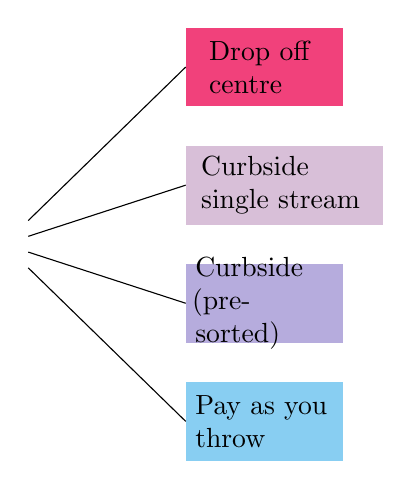
\begin{tikzpicture}
\MindMapOne
%	\fill[color=lime] (0,0) rectangle (4,1) node[pos=.5] {\color{black}``Best'' recycling centre};
%	\fill[color=BurntOrange] (6,2.5) rectangle (8,1.5) node[pos=.5] {\color{black}\begin{minipage}{40pt}\raggedright Most participation\end{minipage}};
%	\fill[color=Goldenrod] (6,0) rectangle (8,1) node[pos=.5] {\color{black}\begin{minipage}{45pt}\raggedright Least cost to the city\end{minipage}};
%	\fill[color=red] (6,-2) rectangle (8,-0.5) node[pos=.5] {\color{black}\begin{minipage}{50pt}\raggedright Processes the most recyclables\end{minipage}};
%	\draw (4,0.75) -- (6,2);
%	\draw (4,0.5) -- (6,0.5);
%	\draw (4,0.25) -- (6,-1.25);
	\fill[color=WildStrawberry!80!white] (10,2.25) rectangle (12,3.25) node[pos=.5] {\color{black}\begin{minipage}{40pt}\raggedright Drop off centre\end{minipage}};	
	\fill[color=Thistle] (10,0.75) rectangle (12.5,1.75) node[pos=.5] {\color{black}\begin{minipage}{60pt}\raggedright Curbside single stream\end{minipage}};	
	\fill[color=Periwinkle!50!white] (10,0.25) rectangle (12,-0.75) node[pos=.5] {\color{black}\begin{minipage}{50pt}\raggedright Curbside (pre-sorted)\end{minipage}};	
	\fill[color=Cerulean!50!white] (10,-2.25) rectangle (12,-1.25) node[pos=.5] {\color{black}\begin{minipage}{50pt}\raggedright Pay as you throw\end{minipage}};
	\draw (8,0.8) -- (10,2.75);	
	\draw (8,0.6) -- (10,1.25);	
	\draw (8,0.4) -- (10,-0.25);	
	\draw (8,0.2) -- (10,-1.75);	
\end{tikzpicture}
\end{center}
\end{example}
\end{siam}

%\begin{figure}[!htbp]
%\begin{tikzpicture}
%	\fill[color=Green] (0,0) rectangle (4,1) node[pos=.5] {\color{black}``Best'' recycling centre};
%	\fill[color=BurntOrange] (6,2.5) rectangle (8,1.5) node[pos=.5] {\color{black}\begin{minipage}{40pt}\raggedright Most participation\end{minipage}};
%	\fill[color=Goldenrod] (6,0) rectangle (8,1) node[pos=.5] {\color{black}\begin{minipage}{45pt}\raggedright Least cost to the city\end{minipage}};
%	\fill[color=red] (6,-2) rectangle (8,-0.5) node[pos=.5] {\color{black}\begin{minipage}{50pt}\raggedright Processes the most recyclables\end{minipage}};
%	\draw (4,0.75) -- (6,2);
%	\draw (4,0.5) -- (6,0.5);
%	\draw (4,0.25) -- (6,-1.25);
%	\fill[color=WildStrawberry] (10,2.25) rectangle (12,3.25) node[pos=.5] {\color{black}\begin{minipage}{40pt}\raggedright Drop off centre\end{minipage}};	
%	\fill[color=Thistle] (10,0.75) rectangle (12.5,1.75) node[pos=.5] {\color{black}\begin{minipage}{60pt}\raggedright Curbside single stream\end{minipage}};	
%	\fill[color=Periwinkle] (10,0.25) rectangle (12,-0.75) node[pos=.5] {\color{black}\begin{minipage}{50pt}\raggedright Curbside (pre-sorted)\end{minipage}};	
%	\fill[color=Cerulean] (10,-2.25) rectangle (12,-1.25) node[pos=.5] {\color{black}\begin{minipage}{50pt}\raggedright Pay as you throw\end{minipage}};
%	\draw (8,0.8) -- (10,2.75);	
%	\draw (8,0.6) -- (10,1.25);	
%	\draw (8,0.4) -- (10,-0.25);	
%	\draw (8,0.2) -- (10,-1.75);	
%\end{tikzpicture}
%\caption{Next step of a mind map.}
%\label{mindmap2}
%\end{figure}


\begin{important}
		There is free online software to help creating a mind map. One such is \href{http://freemind.sourceforge.net}{FreeMind (http://freemind.sourceforge.net)}.
		
		\hfill \qrcode{http://freemind.sourceforge.net}
\end{important}


\begin{graybox}
\begin{minipage}{.75\textwidth}
For more details on creating a mind map, check the book:
\begin{verbatim}
	Math Modeling: Getting Started and Getting Solutions, K. M. Bliss, K. R. Fowler, 
	and B. J. Galluzzo, SIAM, Philadelphia, 2014
\end{verbatim}
\begin{center}
\href{https://m3challenge.siam.org/resources/modeling-handbook}{\tt https://m3challenge.siam.org/resources/modeling-handbook}
\end{center}
\end{minipage}
\hfill
\begin{minipage}{.20\textwidth}
	\hfill\qrcode{https://m3challenge.siam.org/resources/modeling-handbook}	
\end{minipage}
\end{graybox}






	\begin{exercises}
		% Topics:
		% 
	\begin{problist}
		% 
		\prob
		Expand the mind map from the example above by focusing on the other two approaches:
		\begin{enumerate}
			\item Most participation
			\item Processes the most recyclables
		\end{enumerate}

		
	For each part, create a mind map. 
	Focus on the same approach you had for the \hyperref[exercise:define]{questions from the previous module}.

		\prob Help the Canadian Institute of Health Information (CIHI) estimate how significant the outbreak of illnesses will be in the coming year in Canada.
		\prob Create a mathematical model to rank roller coasters according to thrill factor.
		\prob Gas stations offer different prices for gas. I would like to create an app that finds the best gas station to go to. What should ``best'' mean?
		\prob The mayor of Toronto wants to extend the subway line with a new orange line as in \hyperref[p:TTC]{core exercise \ref{p:TTC}}. Is it optimal?
		
		\prob Is it better to buy a car or rent Zipcar, or Car2go?
		
		\prob Help Airbus design the interior of an airplane.

	\end{problist}
\end{exercises}

\end{module}



\begin{lesson}
	\Title{Defining Problem Statement}

	\Heading{Objectives}
	\begin{itemize}
		\item The second step in Mathematical modelling is to construct a representation of how the team will be attempting to solve the problem.
		\item Create a mind map of the problem. This is a structured way to brainstorm possible solutions and their requirements.
	\end{itemize}
	
	\Heading{Motivation} 

\begin{annotation}
	\begin{goals}
	\Goal{Extra Reading}
	Math Modelling: Getting started and getting solutions, Bliss-Fowler-Galluzzo
	
	\hfill \qrcode{https://m3challenge.siam.org/resources/modeling-handbook}	
	\end{goals}
\end{annotation}
	\Heading{Extra Reading} \href{https://m3challenge.siam.org/resources/modeling-handbook}{Math Modelling: Getting started and getting solutions, Bliss-Fowler-Galluzzo}

\end{lesson}




%\newpage


\question
\label{elevatorR}
Consider the elevator problem from question \ref{elevator-define}.


\begin{annotation}
	\begin{notes}
	\begin{itemize}
		\item Students usually come up with more complicated variations:
		\begin{itemize}
			\item Money spent on late employees' salaries
			\item sum of time in minutes that employees are late counting only employees that are at most 15 minutes late
		\end{itemize}
		\item Stick with $T$, a simple first approach
	\end{itemize}	
	\end{notes}
	
\end{annotation}

Your team decides that the mathematical object you will use to show the CEO that you solved or improved the problem is
\begin{itemize}
	\item $T=$ the sum in minutes by which every employee is late.
\end{itemize}

Note that employees that are on time count for 0 minutes (not a negative amount of minutes). \\

Create a mind map for the question: \quad How can $T$ be minimized?


\bookonlynewpage


\question

The city of Toronto decided to tear down the Gardiner expressway. While the demolition is taking place, several key arteries are closed and many intersections are bottled. 
At peak times, a police officer is often posted at this intersection to \emph{optimally} control the traffic lights. 

\begin{parts}
	\item What mathematical meaning can we give to the word optimal in this circumstance? 
	\item Create a mind map for this problem.
\end{parts}




	









\standardonlynewpage


%%%%%%%%%%%%%%%%%%%%%%%%%%%%%%
%
%  MODULE - Making Assumptions
%
%%%%%%%%%%%%%%%%%%%%%%%%%%%%%%



\begin{module}{Making assumptions}
	%\Title{Making Assumptions}
	\label{assumption}

\begin{siam}
	In this module you will learn
\begin{itemize}
	\item that we need to make assumptions to be able to create a model
	\item how to strike a balance between accuracy and solvability
\end{itemize}

\hfill \\




Real problems are complex, so when modelling a real problem mathematically, we must make some assumptions. 

The assumptions that we make will affect the problem we are solving and its difficulty, so we need to strike a balance between:
\begin{itemize}
\item accuracy -- the fewer assumption the better, and
\item solvability -- the more assumptions the better.
\end{itemize}

\begin{annotation}
	\begin{goals}
		When building a mind map, keep track of the assumptions necessary for each step.
	\end{goals}
\end{annotation}

Many assumptions follow naturally when building a mind map. \\


\begin{annotation}
	\begin{goals}
		Remember to justify all your assumptions.
	\end{goals}
\end{annotation}

When figuring which assumption to make, keep in mind the key-factors of the problem and find data when available (usually online). 
If not available, measure data when possible, and if it's not possible, make a reasonable assumption on what the data might look like.

Another thing to keep in mind are \emph{time constraints}. Whether in a class, test, or working in a project, there will be deadlines. Your assumptions should take time constraints into consideration. 



\begin{example}

AN EXAMPLE, PROBABLY BASED ON THE RECYCLING.
	
\end{example}




%\hfill \\

%	\section*{Step D. Parameters or Variables?}\label{D-parvsvar}
%	\addcontentsline{toc}{subsection}{Step D. Parameters or Variables?}
%	
%	
%	
%	When you have defined the problem you want to solve and you have made your (initial) assumptions, it is then time to define some details of the problem.
%	
%	
%	
%	
%	With the problem statement clearly defined and an initial set of assumptions made (a list that will likely get longer), you are ready to start to define the details of your model. Now is the time to pause to ask what
%	is important that you can measure. Identifying these notions as variables, with units and some sense of their range, is key to building the model.
%	The purpose of a model is to predict or quantify something of interest. We refer to these predictions
%	as the outputs of the model. Another term we use
%	for outputs is dependent variables. We will also have independent variables, or inputs to the model. Some quantities in a model might be held constant, in which case they are referred to as model parameters. Let's look at a few simple examples that will help you distinguish between these concepts. We'll also see how they depend on your viewpoint and the problem statement.
%	
%	
%	
%	%There is a clear difference between \emph{variables} and \emph{parameters}. 
%	
%	\begin{definition}[Variables and Parameters]
%	
%	
%	A \emph{variable} represents a model state, and may change during simulation.
%	
%	A \emph{parameter} is commonly used to describe objects statically. A \emph{parameter} is normally a constant in a single simulation, and is changed only when you need to adjust your model behaviour. 
%	\end{definition}
%	
%	%Use a variable instead of a parameter if you need to model some data unit continuously changing over time. Use a parameter instead of a variable if you just need to model some parameter of an object changed only at particular moments of time.
%	
%	
%	
%	\begin{annotation}
%		\begin{goals}
%		\qrcode{https://en.wikipedia.org/wiki/Parameter\#Mathematical\_models}	
%		\end{goals}
%	\end{annotation}
%	\begin{note}{(from Wikipedia)}
%	The quantities appearing in the equations we classify into variables and parameters. The distinction between these is not always clear cut, and it frequently depends on the context in which the variables appear. 
%	
%	Usually a model is designed to explain the relationships that exist among quantities which can be measured independently in an experiment; these are the \emph{variables} of the model. 
%	
%	To formulate these relationships, however, one frequently introduces ``constants'' which stand for inherent properties of nature (or of the materials and equipment used in a given experiment). These are the \emph{parameters}.	
%	\end{note}






%
%
%
%The choice of question in the previous module should determine the \emph{dependent} variable.

%
%The \emph{parameters} are the independent variables in the problem, e.g. the speed of the elevators. The final answer will depend on the parameters in the problem. 
%
%We can estimate the parameters, and sometimes even change them. \\
%
%The \emph{variables} are dependent. This meant that if we change the parameters, the variables will change automatically. 

	\begin{exercises}
		% Topics:
		% 
	\begin{problist}
	\prob
	For each part, you are required to make an estimate for some quantity. Make assumptions and justify them in order to solve the problem.
		\begin{enumerate}
			\item What is the number of piano players in Toronto? \hfill \emph{(Fermi problem)}
			\item How many linear km of roads are there in Toronto?
			\item How much salt the city of Toronto needs for its roads during the Winter?
			\item The skating season in Canada is shortening: What are the key-factors determining its length?
		\end{enumerate}
	\end{problist}
\end{exercises}

\end{siam}
\end{module}
	



\begin{lesson}
	\Title{Making Assumptions}

	\Heading{Objectives}
	\begin{itemize}
		\item The second step in Mathematical modelling is to construct a representation of how the team will be attempting to solve the problem.
		\item Create a mind map of the problem. This is a structured way to brainstorm possible solutions and their requirements.
	\end{itemize}
	
	\Heading{Motivation} 

\begin{annotation}
	\begin{goals}
	\Goal{Extra Reading}
	Math Modelling: Getting started and getting solutions, Bliss-Fowler-Galluzzo
	
	\hfill \qrcode{https://m3challenge.siam.org/resources/modeling-handbook}	
	\end{goals}
\end{annotation}
	\Heading{Extra Reading} \href{https://m3challenge.siam.org/resources/modeling-handbook}{Math Modelling: Getting started and getting solutions, Bliss-Fowler-Galluzzo}

\end{lesson}




%\newpage

\begin{minipage}{.5\textwidth}	
\question
\label{elevator-assumptions}
Consider the elevator problem from \hyperref[elevator-define]{core exercise \ref{elevator-define}}. 


We now give you some technical details about \nobreak{theBigCompany}:

\begin{itemize}
	\item The company occupies the floors 30--33 of the building Place Ville-Marie in Montr\'eal.

	\item Personnel is distributed in the following way: 
	\begin{itemize}
		\item 350 employees in floor 30,
		\item 350 employees in floor 31,
		\item 250 employees in floor 32, 
		\item 150 employees in floor 33.
	\end{itemize}
\end{itemize}

\emph{Note.} Even though these details are fictional, the numbers respect the building code. \\

\emph{Hint.} Focus on a \textbf{few} parameters and variables.
\end{minipage}
\qquad
\begin{minipage}{.5\textwidth}	
\email
\end{minipage}

\begin{parts} 

	\item With your team, decide on what kind of information you would need to have to be able to solve this problem.

	\item Find the relevant information about the elevators (search the internet, by experimentation). Check the reliability of the data you found.

	\item For the relevant information that you cannot obtain, make assumptions. These assumptions should be reasonable and you should be able to justify them.
\end{parts}

\begin{annotation}
	\begin{notes}
		\begin{itemize}
			\item Students usually have trouble starting. 
			\item They usually agree that they have to figure out how elevators work, so you can prompt them to be more specific. 
			
			\item In the end they should come up with questions like these:
			\begin{itemize}
				\item How fast are the elevators?
				\item How much time do elevators take in each floor?
				\item How many floors do elevators stop on their way up?
				\item How many people fit in the elevator?
				\item Should we consider elevator failures?
			\end{itemize}
		\end{itemize}	
	\end{notes}
\end{annotation}




\bookonlynewpage

\hfill

\bookonlynewpage

\question How much would it cost to make a bridge between Toronto and the U.S.?














\standardonlynewpage

%%%%%%%%%%%%%%%%%%%%%%%%%%%%%%
%
%  MODULE - Construction of the Model
%
%%%%%%%%%%%%%%%%%%%%%%%%%%%%%%



\begin{module}{Construct a model}
	%\Title{Construct a model}
	\label{model}

\begin{siam}
	
In this module you will learn
\begin{itemize}
	\item how to build a model based on the previous steps
\end{itemize}

\hfill \\



This is the part of the modelling where we connect all that we have done so far: the problem we defined, the mind map, the assumptions, and all the variables and parameters in a mathematical model to answer the ``mathematical'' problem defined in \hyperref[define]{Step A}.


%When you have defined the problem you want to solve and you have made your (initial) assumptions, it is then time to define some details of the problem.
	
	
With the problem statement clearly defined and an initial set of assumptions made (a list that will likely get longer), you are ready to start to define the details of your model. Now is the time to pause to ask what is important that you can measure. 
Identifying these notions as variables, with units and some sense of their range, is key to building the model.

The purpose of a model is to predict or quantify something of interest. %We refer to these predictions as the outputs of the model. 
	
Creating a model usually means writing down mathematical equations, constructing a graph, analyzing a geometric figure, or do some statistical analysis. \\


\begin{example}
Your team is tasked with finding the best recycling centre (we looked at this example in \hyperref[mindmap]{Step B}) and your  team has chosen to minimize the cost to the city by using drop off centres.

As part of modelling process, your team has made the following assumptions/measurements:
\begin{itemize}
	\item People would be willing to pay \$2.29 to recycle per month or \$0.53 per week
	\item People would make one weekly trip to the centre
	\item Gasoline costs around \$1.26 per litre
	\item On average a passenger car consumes 10 litres per hundred kilometres\\
\end{itemize}

This means that the (one-way) distance people are willing to travel every week to the drop-off centre is
$$
d \;=\; \frac{1}{4.3 \text{ trips/month}} \cdot \frac{\$2.29 / {\text{month}} }{(\$1.26 \text{/L}) \ \cdot\  (0.1 \text{ L / km})} \;=\; 4.2 \text{  km/trip}.
$$

This should help us figure out the best way to place the drop-off centres. \\

The Mathematical model might look like this

\begin{itemize}
	\item Maximize (number of people within a 4.2 km radius of a drop-off centre)
	\item subject to a certain number of drop-off centres (given by the city budget) %\\
\end{itemize}

%\textit{Note. } The model should also include the cost of building a drop off centre.
\end{example}

\begin{graybox}
Assuming that this project was requested for a specific city, the final report should also include some suggested locations for various different budgets.	
\end{graybox}


%\hfill
%
%Sometimes, the mathematical tools necessary to tackle the problem are clear, but often they are not. In those cases it may be helpful to analyze some simple cases.




	\begin{exercises}
		% Topics:
		% 
	\begin{problist}
	\prob
	For each part, create a model to answer the question. Remember all the previous steps.

	\begin{enumerate}
	\item You want to open a piano store in Toronto, where should you open it?
	\item There was a big snow storm in Toronto and the roads need cleaning. How should the city deploy its snow plowers?
	\item The city of Toronto wants to deactivate the Pickering nuclear power plant in favour of renewable power sources. What is the best way to create the same amount of electricity using only renewable sources in the GTA?
	\item Loblaws wants to start an online food delivery service. How should they do it?
	\item The city airport (YTZ) built a tunnel to access the island airport from the city. Before that, they used a ferry. Was building the tunnel a good decision?	
		\end{enumerate}
	\end{problist}
\end{exercises}

\end{siam}

\end{module}



\begin{lesson}
	\Title{Construct a model}

	\Heading{Objectives}
	\begin{itemize}
		\item The second step in Mathematical modelling is to construct a representation of how the team will be attempting to solve the problem.
		\item Create a mind map of the problem. This is a structured way to brainstorm possible solutions and their requirements.
	\end{itemize}
	
	\Heading{Motivation} 

\begin{annotation}
	\begin{goals}
	\Goal{Extra Reading}
	Math Modelling: Getting started and getting solutions, Bliss-Fowler-Galluzzo
	
	\hfill \qrcode{https://m3challenge.siam.org/resources/modeling-handbook}	
	\end{goals}
\end{annotation}
	\Heading{Extra Reading} \href{https://m3challenge.siam.org/resources/modeling-handbook}{Math Modelling: Getting started and getting solutions, Bliss-Fowler-Galluzzo}

\end{lesson}




%\newpage



\begin{minipage}{.5\textwidth}	
\question
Recall the \hyperref[elevator-assumptions]{core exercise \ref{elevator-assumptions}}.

\begin{itemize}
	\item The company occupies the floors 30--33 of the building Place Ville-Marie in Montr\'eal.

	\item Personnel is distributed in the following way: 
	\begin{itemize}
		\item 350 employees in floor 30,
		\item 350 employees in floor 31,
		\item 250 employees in floor 32, 
		\item 150 employees in floor 33.
	\end{itemize}
\end{itemize}

\vspace{2cm}

Write down a mathematical model for this problem.
\label{elevator-model}
\end{minipage}
\qquad
\begin{minipage}{.5\textwidth}	
\email
\end{minipage}

\begin{annotation}
\begin{goals}
	NEED LOTS OF INSTRUCTIONS FOR INSTRUCTORS HERE!
\end{goals}	
\end{annotation}


















\standardonlynewpage


%%%%%%%%%%%%%%%%%%%%%%%%%%%%%%
%
%  MODULE - Model Assessment
%
%%%%%%%%%%%%%%%%%%%%%%%%%%%%%%



\begin{module}{Model Assessment}
	%\Title{Model Assessment}
	\label{analysis}

\begin{siam}
	
In this module you will learn
\begin{itemize}
	\item how to analyze a model
	\item to check the quality of the model
\end{itemize}

\hfill \\



At this point, you have defined a problem statement, and a mind map to help you decide how to approach the problem. You have made assumptions and made note of them and justified them.
You finally created a model to solve the problem.

The next step is to analyze the model.

There are two types of analysis:


\paragraph{\textcolor{cyan}{\textbf{Superficial assessment.}}} Are the units correct? Are the variables and parameters of a reasonable magnitude? Does it behave as expected? Does it make sense?



\paragraph{\textcolor{cyan}{\textbf{In-depth assessment.}}} Once the superficial assessment is verified, we need to understand the model at a deeper level. 

What are the model's strengths? What are its weaknesses?

When you change the inputs of the model, how do the outputs change? This is called {\emph sensitivity analysis}. 


%Next is a simple example adapted from \cite{bliss}.


%\begin{annotation}
%	\begin{goals}
%	\Goal{Desmos Graph}
%	\hfill \qrvideo{https://www.desmos.com/calculator/z9cftzus0z}
%	\end{goals}
%\end{annotation}

\begin{example}\textbf{Modelling the flu}

History of the project:
\begin{itemize}
	\item Split population into two classes: \emph{infected} and \emph{not infected}
	\item Assume that each infected person infects $R$ number of non infected people every $b$ days
	\item Define $I(n) = $ number of infected people after $n$ days
	\item The two previous points imply \quad $I(n + b) = I(n) + R \, I(n)$
	\item We can then conclude that \quad $I(n b) = (1+R)^n \, I(0)$ \hfill (why?) \\
\end{itemize}

After plotting the resulting function $I(n)$ (with $R=5, b=2, I(0)=20$), we can assess our model.
\begin{center}
	\includegraphics*[width=300pt]{images/module5-graph.png}	
\end{center}
\begin{itemize}
	\item \qrvideo{https://www.desmos.com/calculator/deh5qeea20}
\end{itemize}


\emph{Strengths:}
\begin{itemize}
	\item After two days $(b=2)$, there are 6 infected people, so it is following our assumption
	\item The number of infected people increases faster and faster as expected 
	\item The disease spreads at a constant rate. Also on Desmos, check the infection rate $\dfrac{I(n+b)}{I(n)}$
	\item We could find an explicit formula for the number of infected individuals $I(n)$ \\
\end{itemize}


\emph{Weaknesses:}
\begin{itemize}
	\item The model is too simple, so it doesn't model the spread of the flu accurately
	\item The model yields an exponential rate of infection, which is not possible for very long
	\item The model predicts that eventually the disease will spread to everyone
	\item The model assumes that there are only two types of people: infected and susceptible. Do people recover from the disease?
\end{itemize}

\end{example}




After assessing the model, if time allows, it is important to re-think the model and the assumptions made.



	\begin{exercises}
		% Topics:
		% 
	\begin{problist}
	\prob
	Assess the models created in question \ref{models1}:

	\begin{enumerate}
		\item You want to open a piano store in Toronto, where should you open it?
		\item There was a big snow storm in Toronto and the roads need cleaning. How should the city deploy its snow plowers?
		\item The city of Toronto wants to deactivate the Pickering nuclear power plant in favour of renewable power sources. What is the best way to create the same amount of electricity using only renewable sources in the GTA?
		\item Loblaws wants to start an online food delivery service. How should they do it?
		\item The city airport (YTZ) built a tunnel to access the island airport from the city. Before that, they used a ferry. Was building the tunnel a good decision?	
	\end{enumerate}
	\end{problist}
\end{exercises}

\end{siam}

\end{module}



\begin{lesson}
	\Title{Model Assessment}

	\Heading{Objectives}
	\begin{itemize}
		\item The second step in Mathematical modelling is to construct a representation of how the team will be attempting to solve the problem.
		\item Create a mind map of the problem. This is a structured way to brainstorm possible solutions and their requirements.
	\end{itemize}
	
	\Heading{Motivation} 

\begin{annotation}
	\begin{goals}
	\Goal{Extra Reading}
	Math Modelling: Getting started and getting solutions, Bliss-Fowler-Galluzzo
	
	\hfill \qrcode{https://m3challenge.siam.org/resources/modeling-handbook}	
	\end{goals}
\end{annotation}
	\Heading{Extra Reading} \href{https://m3challenge.siam.org/resources/modeling-handbook}{Math Modelling: Getting started and getting solutions, Bliss-Fowler-Galluzzo}

\end{lesson}




%\newpage

\question

Continuing on the \hyperref[elevator-model]{elevator problem}, let us think of this model for the problem.

\textbf{Facts:}
\begin{itemize}
	\item Loading time of people at ground floor = 20 s
	\item Speed of uninterrupted ascent/descent = 1.5 floors/s
	\item Stop time at a floor = 7 s
	\item Number of elevators serving floors 30--33 = 8

	(these elevators serve floors 23-33 = 11 floors)
	
	\item Maximal capacity of elevators = 25 people
\end{itemize}


\textbf{Assumptions:}
\begin{itemize}
	\item Personnel that should start at time $t$, arrive uniformly in the interval $[t-30, t-5]$ in minutes
	\item First arrived, first served
	\item During morning rush hour, elevators don't stop on the way down
	\item Elevators stop only at half the floors they serve
	\item Elevator failures are neglected
	\item Mean number of people per floor is equal to the mean number of people per floor of the BigCompany
	\item Elevators are filled, in average, to 80\% of their capacity
\end{itemize}


\textbf{Model:}
\begin{itemize}
	\item Mean number of people per floor $= d = \dfrac{350+350+250+150}{4} = 275$ people / floor
	\item Number of people on floors served by elevators (11 floors) $= N = d \cdot 11 = 3025$ people
	\item Time $\Delta t$ of one trip

\hfil $\Delta t \quad = \quad $ \framebox{$\substack{\text{loading time on}\\\text{ground floor}}$} 
		$ \;+ \;$ \framebox{$\substack{\text{time of flight}\\\text{ground $\to 33$}}$}
		$ \;+\; $ \framebox{$\substack{\text{time of flight}\\\text{$33 \to$ ground}}$}
		$\;+\; $ \framebox{$\substack{\text{stop time to}\\\text{6 of the 11 floors}}$} $\quad = \quad$ 106 s
		
		\item Number of trips necessary per elevator $= n = \dfrac{3025}{20 \cdot 8} \approx 19$ trips

		\item Time necessary to carry the staff of the BigCompany $= \pmb{t} = \dfrac{19 \cdot 106}{60} = 33 $ minutes
		
		\item Accumulated late time $ = \pmb{T} = 180 \cdot 20 \cdot 8 + 74 \cdot 20 \cdot 8 = 40\,640$ seconds $= $ 11h18m

\end{itemize}

\hfill

\begin{annotation}
	\begin{notes}

Some questions to guide the students:
	\begin{itemize}
	\item What are the strengths?
	\item What are the weaknesses?
	\item Is the result around what you expected?
\end{itemize}	
	
\hfill \\
In case students don't realize that something is wrong:
\begin{itemize}
	\item People start arriving 30 minutes before the starting time, so \emph{almost everybody will be on time?}
	\item Assume that the CEO of the BigCompany is right: people are arriving late! What's wrong with the model?

	\item Which assumptions should be relaxed? Or checked?
	\item If one needs to be replaced, by what?
	\end{itemize}
	
	\end{notes}
\end{annotation}

Your task is to assess this model.
Be ready to report on your assessment.



















\standardonlynewpage


%%%%%%%%%%%%%%%%%%%%%%%%%%%%%%
%
%  MODULE - Report
%
%%%%%%%%%%%%%%%%%%%%%%%%%%%%%%



\begin{module}{Putting it all together}
	%\Title{Putting it all together}
	\label{report}

	\begin{siam}
In this module you will learn
\begin{itemize}
	\item how to put all that you have done together into a well structured report
\end{itemize}

\hfill \\



This is the final stage of the modelling project.

By now, you have started with a mathematically defined problem, with some assumptions, and you have created a mind map to help you navigate the problem.
You have also constructed a model and assessed it to make sure it is sound.

All that we have left is to put all this work together into the form of a report.



The report should consist of two parts:

\begin{enumerate}
	\item \textbf{Summary. } Should be at most one page long, and contain a statement of the problem, a brief description of the methods chose to solve it, and some final results and a conclusion. In this part of the report, you should keep mathematical symbols to a minimum, so the reader gets an idea of what to expect in the remainder of the report without getting bogged down in unfamiliar mathematics.

	\item \textbf{In-depth report. } This is where the details go in. It should start with an introduction to the problem assuming that the reader is not aware of it. It should then be structured according to the steps we did before:
	\begin{itemize}
		\item Optionally, you can include a mind map with a description of how it guided the whole process
		\item Assumptions and variables in the model
		\item The model described in detail
		\item The solution process
		\item The assessment of the model
		\item A conclusion, with a description of the results
	\end{itemize}
\end{enumerate}





\begin{example}
As an example of an excellent report, please read the report from the winning team of the 2019 $M_3C$ challenge:
\begin{itemize}
	\item \qrvideo{https://uoft.me/modelling-app-report}
	\item Read the summary and chapters 1, 2, 5.
\end{itemize}
\end{example}

\end{siam}

\begin{siam2019}


\begin{definition}[Report checklist]

\begin{tabular}{|p{75pt}|p{200pt}|p{125pt}|}
\hline
\textbf{Component}
	& \textbf{Questions about your model and how you made it}
	& \textbf{Useful vocabulary} \\ \hline
\multirow{2}{75pt}[-10pt]{\textbf{Defining the problem}}
	& What is/are the big problem/s that you have been asked to solve?
		& open-ended problem \\ \cline{2-3}
	& What is the specific problem your model is going to solve?
		& specific, focus \\ \hline
\multirow{4}{75pt}[-25pt]{\textbf{Making assumptions}}
	& What ideas did you think about that you decided not to try? 
		& eliminate, prioritize \\ \cline{2-3}
	& What have you assumed in order to solve the problem? Why did you make these choices? 
		& assumption, constraints \\ \cline{2-3} %\hline
%\multirow{2}{75pt}{\textbf{Defining variables}}
	& What quantities are important? Which ones change and which ones stay the same? 
		& variable  \\ \cline{2-3}
	& Where did you find the numbers that you used in your model? 
		& resources, citations \\ \hline
\multirow{2}{75pt}[-15pt]{\textbf{Getting a solution}}
	& What pictures, diagrams or graphs might help people understand your information, model, and results? 
		& diagram, graph, labels  \\ \cline{2-3}
	& What mathematical ideas did you use to describe the situation and solve your problem? 
		& situation  \\ \hline
\multirow{4}{75pt}[-30pt]{\textbf{Model assessment}}
	& How do you know that your calculations are correct? Did you remember to use units (like dollars or metres?) 
		& calculation, unit \\ \cline{2-3}
	& When does your model work? When do you need to be careful because it might not? 
		& limitations  \\ \cline{2-3}
	& How do you know you have a good/useful model? Why does your model make sense? 
		& testing, validation \\ \cline{2-3}
	& If you were going to make your model better, what would you do? 
		& improvement, iteration \\ \hline
\multirow{3}{75pt}[-20pt]{\textbf{Reporting results}}
	& Explain your mathematical model in words and math. 
		& clarity, concision \\ \cline{2-3}
	& What are the strengths and weaknesses of your model?
		& strengths, weaknesses \\ \cline{2-3}
	& What are the 5 most important things for your audience/client to understand about your model and/or solution? 
		& client, audience \\ \hline
\end{tabular}

\hfill \\

This checklist is adapted from

\begin{graybox}
\begin{minipage}{.75\textwidth}
\begin{verbatim}
	GAIMME: Guidelines for Assessment and Instruction in Mathematical
	Modeling Education, Second Edition, Sol Garfunkel and Michelle
	Montgomery, editors, COMAP and SIAM, Philadelphia (2019)
\end{verbatim}
\begin{center}
\url{https://uoft.me/gaimme}
\end{center}
\end{minipage}
\hfill
\begin{minipage}{.20\textwidth}
	\hfill\qrcode{https://uoft.me/gaimme}	
\end{minipage}
\end{graybox}

\end{definition}

	
\end{siam2019}




	\begin{noexercises}

%	\begin{problist}
%	\prob
%	Reports!
%
%	\end{problist}
\end{noexercises}

\end{module}



\begin{lesson}
	\Title{Putting it all together}

	\Heading{Objectives}
	\begin{itemize}
		\item The second step in Mathematical modelling is to construct a representation of how the team will be attempting to solve the problem.
		\item Create a mind map of the problem. This is a structured way to brainstorm possible solutions and their requirements.
	\end{itemize}
	
	\Heading{Motivation} 

\begin{annotation}
	\begin{goals}
	\Goal{Extra Reading}
	Math Modelling: Getting started and getting solutions, Bliss-Fowler-Galluzzo
	
	\hfill \qrcode{https://m3challenge.siam.org/resources/modeling-handbook}	
	\end{goals}
\end{annotation}
	\Heading{Extra Reading} \href{https://m3challenge.siam.org/resources/modeling-handbook}{Math Modelling: Getting started and getting solutions, Bliss-Fowler-Galluzzo}

\end{lesson}







%\newpage

%\question
%Another question to be added here
%
%\newpage





%
%
%
%
%\begin{module}
%	\Title{Putting it all together}
%	\Heading{Textbook} \href{https://m3challenge.siam.org/resources/modeling-handbook}{Math Modelling: Getting started and getting solutions, Bliss-Fowler-Galluzzo}
%	
%	\Heading{Objectives}
%	\begin{itemize}
%		\item Bla bla bla	
%	\end{itemize}
%	
%	\Heading{Motivation} 
%
%
%\end{module}
%
%
%
%
%\section*{Step F. Writing a report}\label{F-report}
%\addcontentsline{toc}{subsection}{Step F. Writing a report}
%









%%%%%%%%%%%%%%%%%%%%%%%%%%%%%%%%%%%%%%%%%%%%%%%%%%%%%%%%%%%%%%%%%%%%%%%%
%
%		Chapter 2 - First-Order Differential Equations
%
%%%%%%%%%%%%%%%%%%%%%%%%%%%%%%%%%%%%%%%%%%%%%%%%%%%%%%%%%%%%%%%%%%%%%%%%





%%%%%%%%%%%%%%%%%%%%%%%%%%%%%%%%%%%%%%%%%%%%%%%%%%%%%%%%%%%%%%%%%%%%%%%%
%
%		Chapter 2 - First-Order ODEs
%
%%%%%%%%%%%%%%%%%%%%%%%%%%%%%%%%%%%%%%%%%%%%%%%%%%%%%%%%%%%%%%%%%%%%%%%%


\begin{topic}[First-Order Differential Equations]



\vfil

\begin{center}
\begin{minipage}{200pt}
	\includegraphics*[width=200pt]{images/chap2-xkcd.png}

	\hfill {\footnotesize (image from \href{https://www.xkcd.com/793/}{xkcd - comic \#793})}
\end{minipage}
\end{center}



\end{topic}




%%%%%%%%%%%%%%%%%%%%%%%%%%%%%%
%
%  MODULE - Introduction
%
%%%%%%%%%%%%%%%%%%%%%%%%%%%%%%


\begin{module}{Introduction to Differential Equations}
%	\Title{Definition}
	\label{ODE-intro}
%	\Heading{Textbook}	
%	\Heading{Objectives}
%	\begin{itemize}
%		\item Bla bla bla	
%	\end{itemize}
%	
%	\Heading{Motivation} 

\begin{lesson}
	\Title{Introduction to Differential Equations}

%	\Heading{Objectives}
%	\begin{itemize}
%		\item The second step in Mathematical modelling is to construct a representation of how the team will be attempting to solve the problem.
%		\item Create a mind map of the problem. This is a structured way to brainstorm possible solutions and their requirements.
%	\end{itemize}
%	
%	\Heading{Motivation} 
%
%\begin{annotation}
%	\begin{goals}
%	\Goal{Extra Reading}
%	Math Modelling: Getting started and getting solutions, Bliss-Fowler-Galluzzo
%	
%	\hfill \qrcode{https://m3challenge.siam.org/resources/modeling-handbook}	
%	\end{goals}
%\end{annotation}
%	\Heading{Extra Reading} \href{https://m3challenge.siam.org/resources/modeling-handbook}{Math Modelling: Getting started and getting solutions, Bliss-Fowler-Galluzzo}
%
\end{lesson}


	In this module you will learn
\begin{itemize}
	\item what is a differential equation
	\item the different types of differential equations
\end{itemize}

\hfill \\[-10pt]


\begin{definition}[Differential Equation]
	A \emph{differential equation} is an equation involving an unknown function and one or more of its derivatives.
\end{definition}


Among differential equations, there are lots of types, that require different approaches, so we need to classify them.

\begin{definition}[Types of Differential Equations]
	There are two main types of differential equations:
	\begin{itemize}
		\item \emph{Ordinary differential equations}, usually denoted as ODEs -- when the unknown function is a function of one variable;
		\item \emph{Partial differential equations}, usually denoted as PDEs -- when the unknown function is a a function of several variables.
	\end{itemize}	
	
	In this book, we are going to focus only on ordinary differential equations.
	
	Among ordinary differential equations, we distinguish them according to:
	\begin{itemize}
		\item \emph{order}: the order of a differential equation is the order of the highest derivative present in the differential equation;
		\item \emph{linear} vs \emph{nonlinear}: A differential equation \quad $F(t,y,y',\ldots,y^{(n)}) = 0$ \quad is called \emph{linear} if $F$ is a linear function of $y, y', \ldots, y^{(n)}$. Linear ODEs have the form
			$$ a_0(t) y(t) + a_1(t) y'(t) + \cdots + a_n(t) y^{(n)}(t) = g(t). $$
			All other differential equations are called \emph{nonlinear}.
	\end{itemize}
\end{definition}

\begin{graybox}
	Roughly, to check whether an ODE is \textbf{linear}, we need to check that:
	\begin{itemize}
		\item The unknown $y$ and its derivatives appear with exponent 1;
		\item The unknown $y$ and its derivatives do not multiply by each other;
		\item The unknown $y$ and its derivatives are not the objects of other functions -- there are no occurrences of things like $\sin(y)$ or $e^{y'}$, $\ln(y'')$, $\sqrt{y^{(3)}}$, etc.
	\end{itemize}
\end{graybox}

In general, when tackling a differential equation, linear ODEs are easier to solve and study than nonlinear. 

In the following chapters, observe how the methods and theory for linear ODEs is much more developed. Nonlinear ODEs are usually tackled on a case-by-case basis, and there is no theory that applies to a class of nonlinear ODEs.

Fortunately, many important problems are modelled by linear equations. \\

A common approach to nonlinear problems is to ``transform'' them into a linear problem. This means that the new linear problem is easier to study, but will be an approximation of the original problem, and often that approximation is only reasonable within some restricted conditions.

\begin{example}
Consider the nonlinear ODE
$$y' = -\sin(y).$$

This is a nonlinear ODE. However, by Taylor's Theorem, we can approximate the function $\sin(y)$ by $y$, as long as $|y|$ is very small.

So we can say that the solution of the original solution is very close to the solution of
$$ y' = -y,$$
as long as $|y|$ is very small.
\end{example}






%	\input{modules/module07-defs-exercises.tex}

\end{module}


















\newpage


%%%%%%%%%%%%%%%%%%%%%%%%%%%%%%
%
%  MODULE - Solutions
%
%%%%%%%%%%%%%%%%%%%%%%%%%%%%%%



\begin{module}{Solutions of Differential Equations}
	%\Title{Solutions}
	\label{intro-sols}

	In this module you will learn
\begin{itemize}
	\item what is a solution of a differential equation
	\item the difference between a solution and an integral curve
\end{itemize}

\hfill \\[-10pt]

Assume that we have found a differential equation that models a situation.
Often the goal is to figure out what happens, so we usually attempt to either solve the differential equation and obtain a solution or to find an approximation for the solution.

In this module, we will discuss solutions in more detail.

\begin{definition}[Solution]
	Given a differential equation, a \emph{solution} is a differentiable function that satisfies the differential equation.
\end{definition}

\begin{example}
Consider the differential equation
$$
t \frac{du}{dt} = u + t^2 \cos(t).
$$

Then the function 
$$
u(t) = t\sin(t)
$$
is a solution, because
$$
t \frac{du}{dt} = t \big( \sin(t) + t \cos(t) \big) = t \sin(t) + t^2 \cos (t) = u + t^2 \cos(t).
$$
\end{example}



\begin{definition}[Integral curve]
	We can represent all the solutions geometrically as an infinite family of curves. These curves are called \emph{integral curves}.
\end{definition}

\begin{example}\label{sols-ex}
Consider the initial-value problem
$$
\begin{cases}
	\dfrac{dy}{dx}=-\dfrac{x}{y} \\
	y(0)=-3
\end{cases}
$$
Then, we can check that curves of the form $x^2 + y^2 = C$ satisfy this differential equation.

This gives us the solution
$$
y(x) = - \sqrt{9 - x^2}.
$$

However, the integral curve for this initial-value problem is the curve
$$
x^2 + y^2 = 9
$$


\begin{center}
\begin{tabular}{cc}
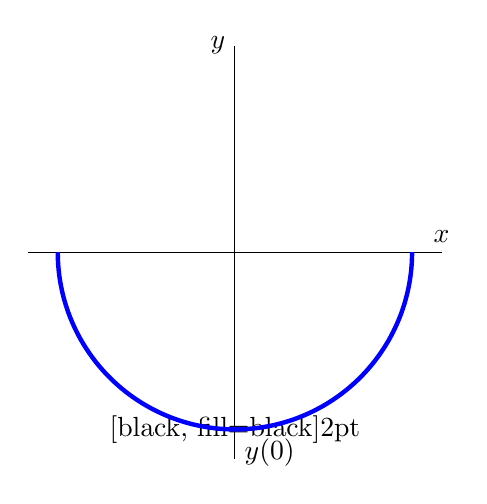
\begin{tikzpicture}[xscale=0.75,yscale=0.75]
	\draw[-{\seta}] (-3.5,0) -- (3.5,0) node[above] {$x$};
	\draw[-{\seta}] (0,-3.5) -- (0,3.5) node[left] {$y$};
	\draw[] (0,-3) node {\tikzcircle[black, fill=black]{2pt}};
	\draw[] (0,-3) node[below right] {$y(0)$};
  \draw[samples=100,ultra thick,domain=0:180,smooth,variable=\t,blue] plot ({3*cos(\t)},{-3*sin(\t)});
\end{tikzpicture}
	& 
	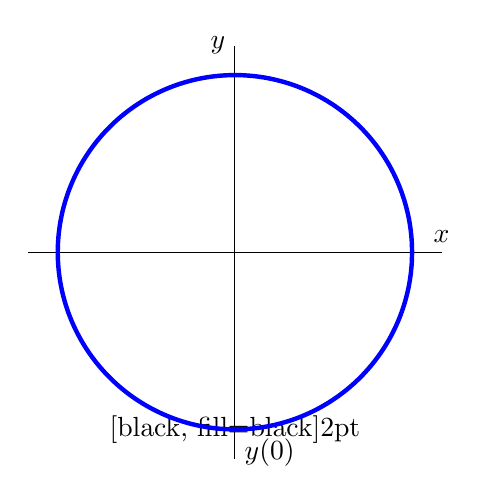
\begin{tikzpicture}[xscale=0.75,yscale=0.75]
		\draw[-{\seta}] (-3.5,0) -- (3.5,0) node[above] {$x$};
		\draw[-{\seta}] (0,-3.5) -- (0,3.5) node[left] {$y$};
		\draw[] (0,-3) node {\tikzcircle[black, fill=black]{2pt}};
		\draw[] (0,-3) node[below right] {$y(0)$};
	  \draw[samples=100,ultra thick,domain=0:360,smooth,variable=\t,blue] plot ({3*cos(\t)},{-3*sin(\t)});
	\end{tikzpicture}

	\\
Solution of the initial-value problem
	& Integral curve for the initial-value problem
\end{tabular}
\end{center}





\end{example}



	\begin{exercises}
		% Topics:
		% 
	\begin{problist}
	\prob Check that curves of the form $x^2 + y^2 = C$ satisfy the differential equation $\dfrac{dy}{dx} = -\dfrac{x}{y}$.
	
	
	\prob Is the piecewise-defined function
	$$
	y(x) = \begin{cases}
 		-x^2 & \text{ if } x< 0 \\
 		x^2 & \text{ if } x \geq 0		
	\end{cases}
	$$
	a solution of the differential equation $xy'-2y=0$ on $(-\infty,\infty)$?
	
	
	\prob Consider the differential equation
	$$ y^{(4)} - 8y^{3)} + 26 y'' - 40y'+25y=0.$$
	
	\begin{enumerate}
		\item Is $y=4 e^{2x}\sin(x)$ a solution?
		\item Is $y=-8 x e^{2x}\cos(x)$ a solution?
		\item For the two function above, if they are solutions, what are initial conditions of the form
			\begin{itemize}
				 \item[] $y(0) =$
				 \item[] $y'(0) =$
				 \item[] $y''(0) =$
				 \item[] $y'''(0) =$
			\end{itemize}
			that the solution satisfies?
	\end{enumerate}


	\prob Consider the functions
	\begin{align*}
		f(x) & = 3x + x^2 	& g(x) & = e^{-7x} \\
		h(x) & = \sin(x) 	& j(x) & = \sqrt{x} \\
		k(x) & = 8 e^{3x}	& \ell(x) & = -2 \cos(x)
	\end{align*}
	
	Match each differential to one or more functions which are solutions.
	
	\begin{enumerate}
		\item $y'=3y$
		\item $y''+9y'+14y=0$
		\item $y''+y=0$
		\item $2x^2y'' + 3xy'=y$
	\end{enumerate}
	
	
	
	\prob Consider the differential equation $u' = -2(u-10)$.
	
	\begin{enumerate}
		\item Check that the curves of the form $u = 10 + C e^{-2t}$ satisfy the differential equation.
		\item Sketch one solution of the differential equation.
		\item Sketch all the integral curves for the differential equation.
		\item What is the difference between a solution passing through the point $(1,20)$ and an integral curve passing through the same point?
	\end{enumerate}


	\prob Consider the differential equation $y'\big( 3y^2-1\big) = 1$.
	
	\begin{enumerate}
		\item Check that the curves of the form $y^3-y=x+C$ satisfy the differential equation.
		\item Sketch the solution of the differential equation that passes through $(1,1)$.
		\item Sketch the integral curve for the differential equation that passes through $(1,1)$.
		\item What is the difference between a solution passing through the point $(1,1)$ and an integral curve passing through the same point?
		\item Repeat (b)--(d) with the points $(1,0)$ and $(1,-1)$ instead of $(1,1)$.
	\end{enumerate}


	\prob Consider the ODE \quad $y'(t) = \big(y(t)\big)^2$ \quad .
	One of these two graphs {\bf cannot} describe the solution. 
	Which one? 
	
	
	\begin{center}
	\begin{tikzpicture}
		\draw[-{\seta}] (-1,0) -- (3,0) node[above] {$t$};
		\draw[-{\seta}] (0,-3) -- (0,1) node[left] {$y$};
		\draw[ultra thick,domain=0.5:2.5,smooth,variable=\x,blue] plot ({\x},{(\x*\x-5)/3-1});
	\end{tikzpicture}
	\hfil
	\begin{tikzpicture}
		\draw[-{\seta}] (-1,0) -- (3,0) node[above] {$t$};
		\draw[-{\seta}] (0,-3) -- (0,1) node[left] {$y$};
		\draw[ultra thick,domain=0.5:2.5,smooth,variable=\x,blue] plot ({\x},{-((\x-3.5)^2)/4-0.25});
	\end{tikzpicture}	
	\end{center}

	\prob We seek a first-order ordinary differential equation \quad $y' = f(\pmb{y})$ \quad whose solutions satisfy
	$$
	\begin{cases}
	y(x)  \mbox{ is concave up if } y < 1 \\
	y(x) \mbox{ is concave down if } y > 1
	\end{cases}
	$$
	%
	Write down or graph a function $f(y)$ that would produce such solutions.

	
	\end{problist}
\end{exercises}

\end{module}



\begin{lesson}
	\Title{Solutions of Differential Equations}

%	\Heading{Objectives}
%	\begin{itemize}
%		\item The second step in Mathematical modelling is to construct a representation of how the team will be attempting to solve the problem.
%		\item Create a mind map of the problem. This is a structured way to brainstorm possible solutions and their requirements.
%	\end{itemize}
%	
%	\Heading{Motivation} 
%
%\begin{annotation}
%	\begin{goals}
%	\Goal{Extra Reading}
%	Math Modelling: Getting started and getting solutions, Bliss-Fowler-Galluzzo
%	
%	\hfill \qrcode{https://m3challenge.siam.org/resources/modeling-handbook}	
%	\end{goals}
%\end{annotation}
%	\Heading{Extra Reading} \href{https://m3challenge.siam.org/resources/modeling-handbook}{Math Modelling: Getting started and getting solutions, Bliss-Fowler-Galluzzo}
%
\end{lesson}




\newpage

\question

Which of these shows solutions of $y' = (x-1)(x+1) = x^2 - 1$ ?

\newlength{\len}
%\setlength{\len}{120pt}
%\begin{tabular}{ccc}
%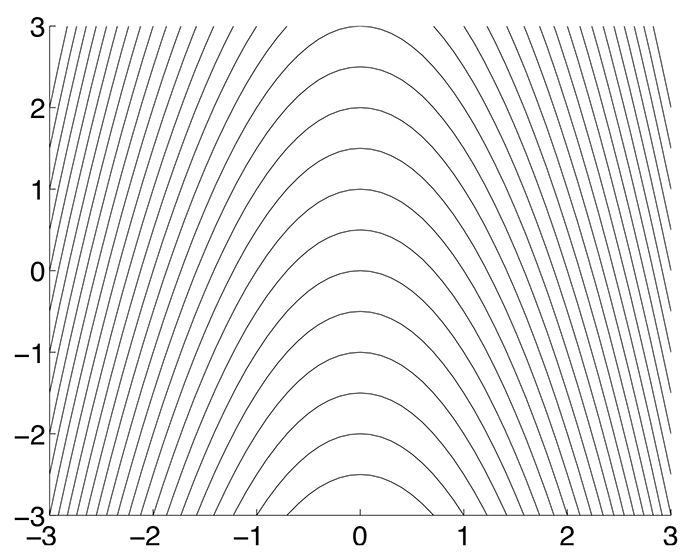
\includegraphics[width=\len]{images/module8-figs-6-small.png}
%	& 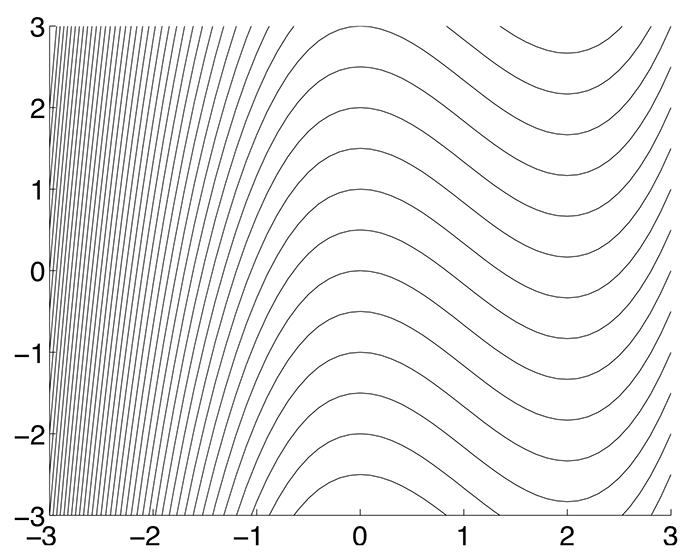
\includegraphics[width=\len]{images/module8-figs-3-small.png}
%	& \includegraphics[width=\len, page=2]{images/module8-figs-2-small.png} \\
%A & B & C \\[15pt]
%%
%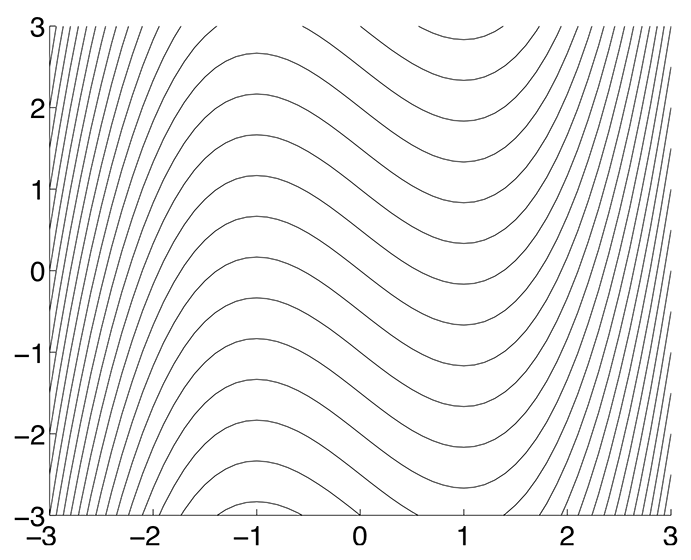
\includegraphics[width=\len]{images/module8-figs-1-small.png}
%	& 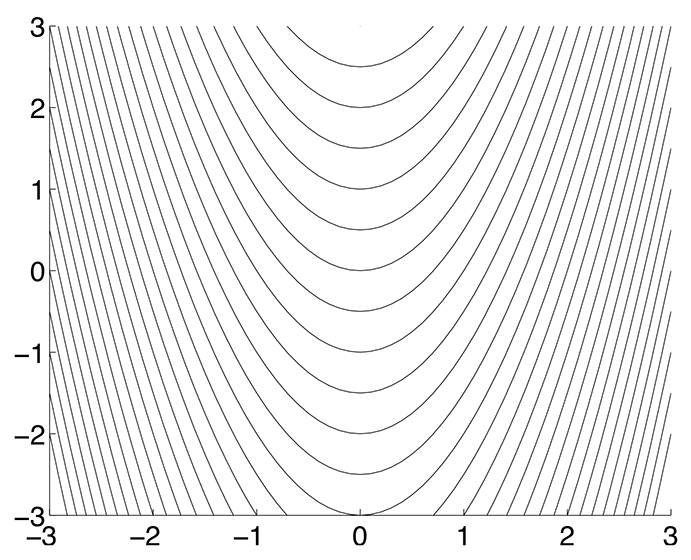
\includegraphics[width=\len]{images/module8-figs-5-small.png}
%	& 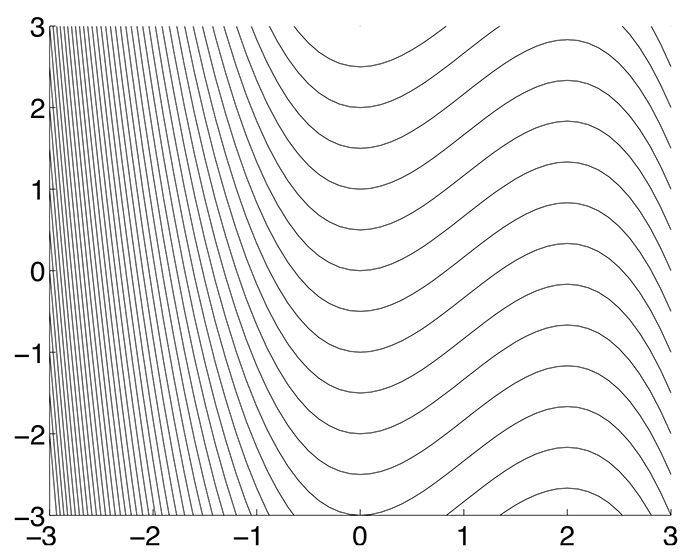
\includegraphics[width=\len]{images/module8-figs-4-small.png} \\
%D & E & F \\
%\end{tabular}


\def\modeightA{
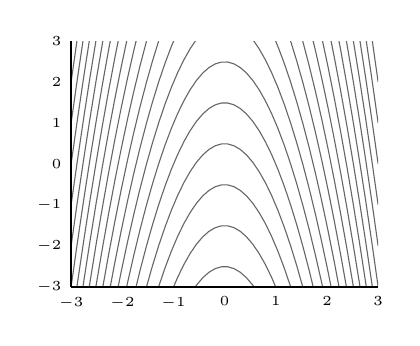
\begin{tikzpicture}[scale=0.65,yscale=0.8]
    \begin{scope}
	    \clip (-3,-3) rectangle (3,3);
		\foreach \k in {-9,-7, ..., 31} {
	      \draw[samples=50,domain=-3:3,variable=\x,color=gray!80!black] plot ({\x},{(\k-3*(\x*\x))/2});
	    }
    \end{scope}
    \draw[thick] (-3,-3) -- (-3,3);
    \draw[thick] (-3,-3) -- (3,-3);
    \foreach \k in {-3,-2, ..., 3} {
      \draw ({\k,-3}) node[below] {\tiny $\k$};
      \draw ({-3,\k}) node[left] {\tiny $\k$};
    }
\end{tikzpicture}
}

\def\modeightB{
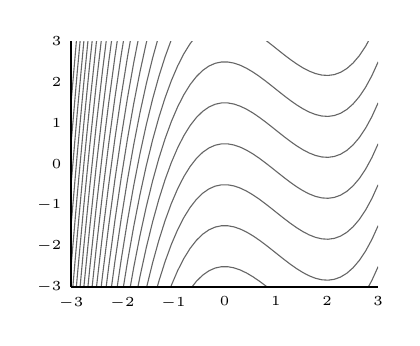
\begin{tikzpicture}[scale=0.65,yscale=0.8]
    \begin{scope}
	    \clip (-3,-3) rectangle (3,3);
		\foreach \k in {-9,-7, ..., 39} {
	      \draw[samples=50,domain=-3:3,variable=\x,color=gray!80!black] plot ({\x},{((\x*\x*\x)/3-(\x*\x)+\k/2)});
    	}
    \end{scope}
    \draw[thick] (-3,-3) -- (-3,3);
    \draw[thick] (-3,-3) -- (3,-3);
    \foreach \k in {-3,-2, ..., 3} {
      \draw ({\k,-3}) node[below] {\tiny $\k$};
      \draw ({-3,\k}) node[left] {\tiny $\k$};
    }
\end{tikzpicture}
}

\def\modeightC{
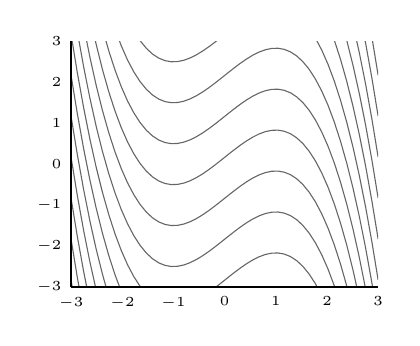
\begin{tikzpicture}[scale=0.65,yscale=0.8]
    \begin{scope}
	    \clip (-3,-3) rectangle (3,3);
		\foreach \k in {-15,-13, ..., 29} {
	      \draw[samples=50,domain=-3:3,variable=\x,color=gray!80!black] plot ({\x},{-(((\x+1)*(\x+1)*(\x+1))/3-((\x+1)*(\x+1))+\k/2)});
    	}
    \end{scope}
    \draw[thick] (-3,-3) -- (-3,3);
    \draw[thick] (-3,-3) -- (3,-3);
    \foreach \k in {-3,-2, ..., 3} {
      \draw ({\k,-3}) node[below] {\tiny $\k$};
      \draw ({-3,\k}) node[left] {\tiny $\k$};
    }
\end{tikzpicture}
}

\def\modeightD{
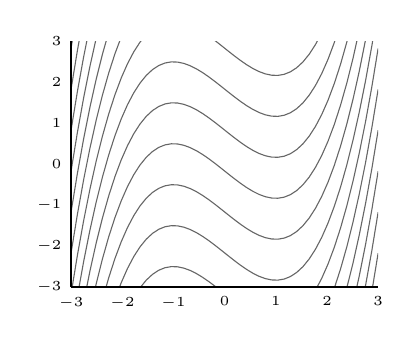
\begin{tikzpicture}[scale=0.65,yscale=0.8]
    \begin{scope}
	    \clip (-3,-3) rectangle (3,3);
		\foreach \k in {-15,-13, ..., 29} {
	      \draw[samples=50,domain=-3:3,variable=\x,color=gray!80!black] plot ({\x},{(((\x+1)*(\x+1)*(\x+1))/3-((\x+1)*(\x+1))+\k/2)});
    	}
    \end{scope}
    \draw[thick] (-3,-3) -- (-3,3);
    \draw[thick] (-3,-3) -- (3,-3);
    \foreach \k in {-3,-2, ..., 3} {
      \draw ({\k,-3}) node[below] {\tiny $\k$};
      \draw ({-3,\k}) node[left] {\tiny $\k$};
    }
\end{tikzpicture}
}

\def\modeightE{
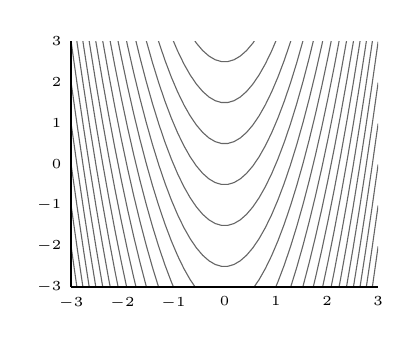
\begin{tikzpicture}[scale=0.65,yscale=0.8]
    \begin{scope}
	    \clip (-3,-3) rectangle (3,3);
		\foreach \k in {-9,-7, ..., 31} {
	      \draw[samples=50,domain=-3:3,variable=\x,color=gray!80!black] plot ({\x},{-(\k-3*(\x*\x))/2});
	    }
    \end{scope}
    \draw[thick] (-3,-3) -- (-3,3);
    \draw[thick] (-3,-3) -- (3,-3);
    \foreach \k in {-3,-2, ..., 3} {
      \draw ({\k,-3}) node[below] {\tiny $\k$};
      \draw ({-3,\k}) node[left] {\tiny $\k$};
    }
\end{tikzpicture}
}

\def\modeightF{
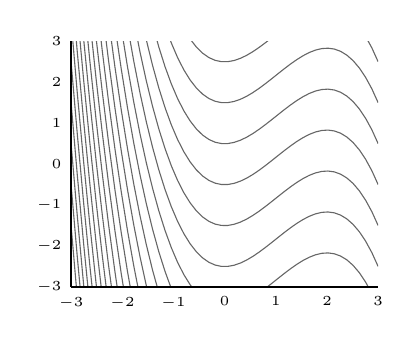
\begin{tikzpicture}[scale=0.65,yscale=0.8]
    \begin{scope}
	    \clip (-3,-3) rectangle (3,3);
		\foreach \k in {-9,-7, ..., 39} {
	      \draw[samples=50,domain=-3:3,variable=\x,color=gray!80!black] plot ({\x},{(-(\x*\x*\x)/3+(\x*\x)-\k/2)});
    	}
    \end{scope}
    \draw[thick] (-3,-3) -- (-3,3);
    \draw[thick] (-3,-3) -- (3,-3);
    \foreach \k in {-3,-2, ..., 3} {
      \draw ({\k,-3}) node[below] {\tiny $\k$};
      \draw ({-3,\k}) node[left] {\tiny $\k$};
    }
\end{tikzpicture}
}


\begin{tabular}{ccc}
\modeightA
	& \modeightB
	& \modeightC \\
A & B & C \\[15pt]
%
\modeightD
	& \modeightE
	& \modeightF \\
D & E & F \\
\end{tabular}



\bookonlynewpage


\question

We seek a first-order ordinary differential equation 
\quad $y' = f(x)$ \quad 
whose solutions satisfy
$$
\begin{cases}
y(x)  \mbox{ is increasing if } x<2 \\
y(x) \mbox{ is decreasing if } 2 < x < 4 \\
y(x) \mbox{ is increasing if } x > 4
\end{cases}
$$
%
Write down or graph an $\pmb{f(x)}$ that would produce such solutions.




\bookonlynewpage

\question

Consider the ODE \quad $y'(t) = \big(y(t)\big)^2$ \quad .
Which of the following is true?
	
\begin{parts}
	\item $y(t)$ must always be positive
	\item $y(t)$ must always be negative \\[5pt]

	\item $y(t)$ must always be decreasing
	\item $y(t)$ must always be increasing
\end{parts}




\bookonlynewpage

\question Consider the differential equation $2xy'=y$.
	
	\begin{parts}
		\item Check that the curves of the form $y^2 + C x = 0$ satisfy the differential equation.
		\item Sketch one solution of the differential equation.
		\item Sketch all the integral curves for the differential equation.
		\item What is the difference between a solution passing through the point $(1,-1)$ and an integral curve passing through the same point?
	\end{parts}








%%%%%%%%%%%%%%%%%%%%%%%%%%%%%%%%%%%%%%%%%%%%%%%%%%%%%%%%%%%%%%%%%%%%%%%%
%		Slope Fields



%%%%%%%%%%%%%%%%%%%%%%%%%%%%%%
%
%  MODULE - Slope Fields
%
%%%%%%%%%%%%%%%%%%%%%%%%%%%%%%



\begin{module}{Slope Fields}
	%\Title{Slope Fields}
	\label{intro-slopefields}

	In this module you will learn
\begin{itemize}
	\item what is a slope field
	\item how to sketch a slope field
	\item to interpret a slope field
\end{itemize}

\hfill \\

As we saw in the previous module, once we have found a differential equation that models a situation, we often want to figure out what happens to the solution.

In this module, we will focus on getting an idea of the solutions and integral curves using what is called a \textbf{slope field}.





\begin{definition}[Slope field] Consider the equation $y' = f(x,y)$.
If we evaluate $f(x,y)$ over a rectangular grid of points, and we draw an arrow at each point $(x,y)$ of the grid with slope $f(x,y)$, then the collection of all the arrows is called a \emph{slope field}.
\end{definition}

\begin{graybox}
	
We can sketch Slope Fields with Wolfram Alpha.

For a differential equation $\dfrac{dy}{dx} = f(x,y)$, we need to input
\begin{itemize}
	\item Vector Field: $(1, f(x,y))$.
\end{itemize}

\url{http://www.wolframalpha.com/input/?i=slope+field}
\hfill \qrcode{http://www.wolframalpha.com/input/?i=slope+field}	
\end{graybox}





\begin{example}
Let us take an \hyperlink{sols-ex}{example from the previous module}.

Consider the initial-value problem
$$
\begin{cases}
	\dfrac{dy}{dx}=-\dfrac{x}{y} \\
	y(0)=-3
\end{cases}
$$

We can use this definition to sketch the slope field for the differential equation $ \dfrac{dy}{dx} = -\dfrac{x}{y}$.

We now sketch this slope field with Desmos:

\url{https://www.desmos.com/calculator/scmz6ps0or} \hfill \qrcode{https://www.desmos.com/calculator/scmz6ps0or}

Now notice that the arrows have the slope of a solution. This means that solutions will be tangent to the arrows, so we can \emph{roughly} trace the solution by following the arrows.

Below, we did just that starting with the point $(0,-3)$.

\setlength{\len}{175pt}
\begin{center}
%\begin{figure}
%\includegraphics*[width=\len]{images/module9-slopefield-ex1.png}
%\hfil
\begin{tabular}{ccc}
\includegraphics*[width=\len]{images/module9-slopefield-ex1-sol.png}
 & & 
\includegraphics*[width=\len]{images/module9-slopefield-ex1-intcurve.png}\\
approximated solution & & approximated integral curve
\end{tabular}
%\caption{Slope Field for the differential equation $\frac{dy}{dx} = -\frac{x}{y}$.
%\label{mod9-slopefield1}
%\end{figure}
\end{center}

\textbf{\textcolor{orange}{Important. }} Remember that this gives us only an approximation of the solution and integral curve. From the approximation, we can tell that the solution seems circular, but we still need to show that it is so.

\end{example}



%\setlength{\len}{150pt}
%\hspace{-1.35cm}\begin{tabular}{ccc}
%\includegraphics*[width=\len]{figures/0101_dirfield_rocket.png}
%	& \includegraphics*[width=\len]{figures/0101_intcurves_rocket.png} 
%	& \includegraphics*[width=\len]{figures/0101_rocket_pos.png} \\
%Direction field for $u$
%	& Approximations of $u$
%	& Solution $u(t)$
%\end{tabular}


%
%This particular one is:
%\href{http://www.wolframalpha.com/input/?i=direction+field+calculator&f1=%7B1%2C-9.8*x-0.75*y%2B10%7D%2Fsqrt(1%2B(-9.8*x-0.75*y%2B10)%5E2)&f=VectorPlot.vectorfunction%5Cu005f%7B1%2C-9.8*x-0.75*y%2B10%7D%2Fsqrt(1%2B(-9.8*x-0.75*y%2B10)%5E2)&f2=x&f=VectorPlot.vectorplotvariable1%5Cu005fx&f3=0&f=VectorPlot.vectorplotlowerrange1%5Cu005f0&f4=2&f=VectorPlot.vectorplotupperrange1_2&f5=y&f=VectorPlot.vectorplotvariable2%5Cu005fy&f6=0&f=VectorPlot.vectorplotlowerrange2%5Cu005f0&f7=4&f=VectorPlot.vectorplotupperrange2%5Cu005f4}{\tt Click Here}
%\hfill \qrcode{http://www.wolframalpha.com/input/?i=direction+field+calculator&f1=%7B1%2C-9.8*x-0.75*y%2B10%7D%2Fsqrt(1%2B(-9.8*x-0.75*y%2B10)%5E2)&f=VectorPlot.vectorfunction%5Cu005f%7B1%2C-9.8*x-0.75*y%2B10%7D%2Fsqrt(1%2B(-9.8*x-0.75*y%2B10)%5E2)&f2=x&f=VectorPlot.vectorplotvariable1%5Cu005fx&f3=0&f=VectorPlot.vectorplotlowerrange1%5Cu005f0&f4=2&f=VectorPlot.vectorplotupperrange1_2&f5=y&f=VectorPlot.vectorplotvariable2%5Cu005fy&f6=0&f=VectorPlot.vectorplotlowerrange2%5Cu005f0&f7=4&f=VectorPlot.vectorplotupperrange2%5Cu005f4}



\begin{video}
\begin{itemize}
	\item \qrvideo{https://youtu.be/MI2xCwBekX4}
	\item \qrvideo{https://youtu.be/8Amgakx5aII}
\end{itemize}	
\end{video}



	\begin{exercises}
		% Topics:
		% 
	\begin{problist}
	\prob Use Wolfram Alpha, Desmos, or another software to sketch the slope field for the following differential equations. Then roughly trace different solutions.
	\begin{enumerate}
		\item $y'=2y-x$
		\item $y'=xy$
		\item $y'=\cos(y)$
		\item $y'=\frac12+\cos(y)$
		\item $y'=1+\cos(y)$
		\item $y'=2+\cos(y)$
		\item $y'=\sin(xy)$
		\item $y'=\tan(x+y)$
	\end{enumerate}
	
	\prob Sketch a slope field for the following differential equation
	$$ y'=f(x,y)$$
	where 
	$$
	f(x,y) = \begin{cases}
 		-x & \text{ if } x< 1 \\
 		y & \text{ if } x \geq 1		
	\end{cases}
	$$

	\prob Sketch a slope field for the following differential equation
	$$ y'=f(x,y)$$
	where the function $f(x,y)$ satisfies all of the following properties:
	\begin{enumerate}
		\item $f(x,y)$ is continuous
		\item $f(x,y) > 0$ when $x>1$ and $y>1$
		\item $f(x,y) < 0$ when $x<-1$ and $y<-1$
		\item $f(x,y)$ depends only on $x$ when $x<-1$ and $y>1$
		\item $f(x,y)$ depends only on $y$ when $x>1$ and $y<-1$
	\end{enumerate}
	
	
	\prob 
		\begin{enumerate}
			\item On the slope field from the previous problem, show that there must exist a smooth continuous curve with horizontal lines.

			\item Show that the curve divides the $(x,y)$ plane in two parts.

		\end{enumerate}
	
	


	\prob Consider a differential equation 
	$$ y'=f(x,y)$$
	where the solutions satisfy
	$$ \lim_{x\to \infty} y(x) = 1.$$

	\begin{enumerate}
		\item What property must the slope field satisfy?

		\item Sketch a possible slope field for this differential equation.
	\end{enumerate}
	
	\end{problist}
\end{exercises}

\end{module}



\begin{lesson}
	\Title{Slope Fields}

	\Heading{Objectives}
	\begin{itemize}
		\item The second step in Mathematical modelling is to construct a representation of how the team will be attempting to solve the problem.
		\item Create a mind map of the problem. This is a structured way to brainstorm possible solutions and their requirements.
	\end{itemize}
	
	\Heading{Motivation} 

\begin{annotation}
	\begin{goals}
	\Goal{Extra Reading}
	Math Modelling: Getting started and getting solutions, Bliss-Fowler-Galluzzo
	
	\hfill \qrcode{https://m3challenge.siam.org/resources/modeling-handbook}	
	\end{goals}
\end{annotation}
	\Heading{Extra Reading} \href{https://m3challenge.siam.org/resources/modeling-handbook}{Math Modelling: Getting started and getting solutions, Bliss-Fowler-Galluzzo}

\end{lesson}




\newpage

\question
\begin{minipage}{.7\textwidth}
	A catapult throws a projectile into the air and we track the height (in metres) of the projectile from the ground as a function $y(t)$, where $t$ is the time (in seconds) that elapsed since the object was launched from the catapult. \\

	Then, the slope fields for $y(t)$ and $y'(t)$ are shown below:
\end{minipage}\hfill
\begin{minipage}{100pt}
	\includegraphics*[width=100pt]{images/module9-catapult.pdf}	
\end{minipage}






\setlength{\len}{200pt}
\begin{tabular}{cc}
\includegraphics*[height=\len]{images/module9-y.png}
	& \includegraphics*[height=\len]{images/module9-yprime.png} \\
Slope field for $y(t)$
	& Slope field for $y'(t)$
\end{tabular}

\hfill {\footnotesize(These slope fields were created using WolframAlpha)} \\

\begin{parts}
	\item On the slope field, sketch a \emph{possible} solution.	
	\item Consider the graph of $y(t)$. Does it form a parabola? Justify your answer.
\end{parts}

\begin{annotation}
	\begin{Goals}
		Students should think about the initial conditions.
		What is a possible value for $y(0)$? What is a possible value for $y'(0)$?
		Then sketch a possible solution that starts at those values. \\
		
		The equilibrium in the slope field for $y'(t)$ is called \emph{terminal velocity}. Some students might be able to identify it.
	\end{Goals}
\end{annotation}





\bookonlynewpage



\question Sketch the slope field for the following differential equations. 

\begin{parts}
	\item $y'=x$

\begin{annotation}
	\begin{Goals}
		The goal is not to be very accurate, but to capture the symmetry of each of these slope fields.
	\end{Goals}
	
\end{annotation}

	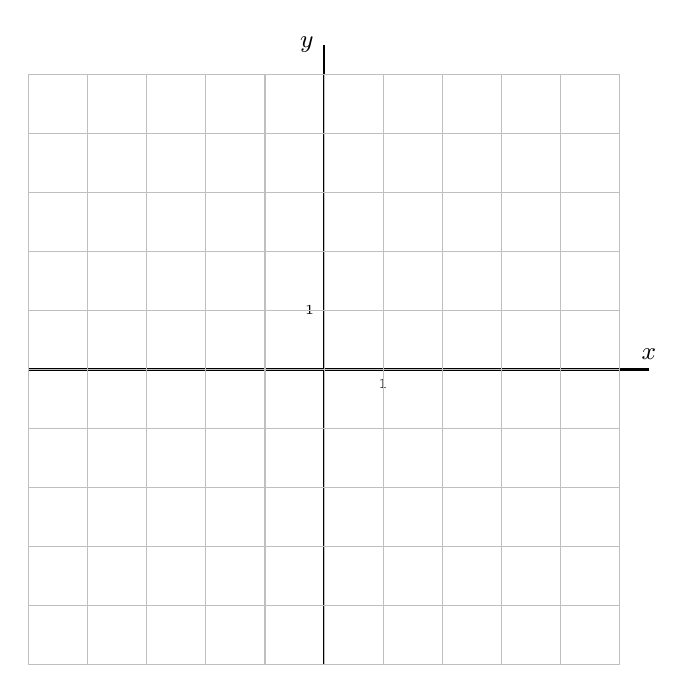
\begin{tikzpicture}[xscale=0.75,yscale=0.75]
		\draw[thick,-{\seta}] (-5,0) -- (5.5,0) node[above] {\small $x$};
		\draw[thick,-{\seta}] (0,-5) -- (0,5.5) node[left] {\small $y$};
		\draw[] (1,0) node[below] {\tiny 1};
		\draw[] (0,1) node[left] {\tiny 1};
		\draw[step=1,lightgray,thin] (-5,-5) grid (5,5);
	\end{tikzpicture}
	
	
\vfil	
	
	\item $y'=y^2$	

	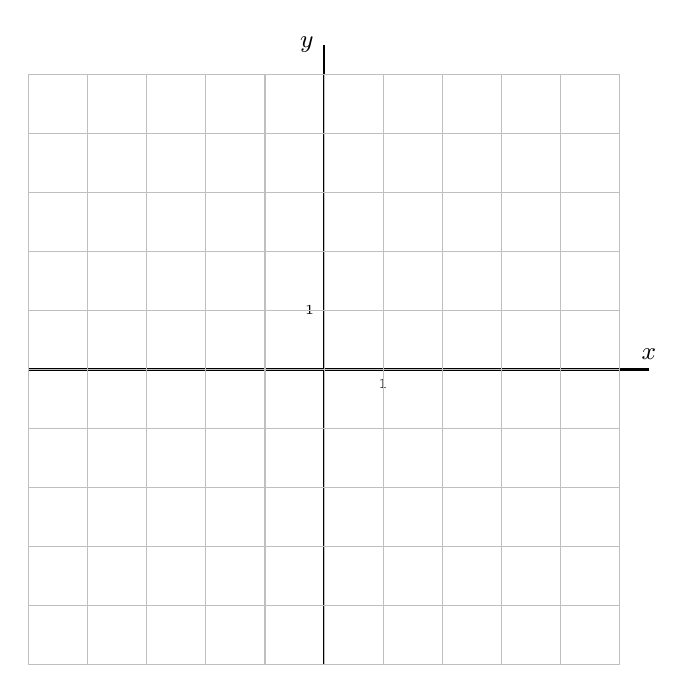
\begin{tikzpicture}[xscale=0.75,yscale=0.75]
		\draw[thick,-{\seta}] (-5,0) -- (5.5,0) node[above] {\small $x$};
		\draw[thick,-{\seta}] (0,-5) -- (0,5.5) node[left] {\small $y$};
		\draw[] (1,0) node[below] {\tiny 1};
		\draw[] (0,1) node[left] {\tiny 1};
		\draw[step=1,lightgray,thin] (-5,-5) grid (5,5);
	\end{tikzpicture}

\end{parts}



\bookonlynewpage

\question Consider the following slope fields:


\setlength{\len}{150pt}
\begin{tabular}{ccc}
	\includegraphics*[height=\len]{images/module9-graph1}
		& \includegraphics*[height=\len]{images/module9-graph2}
		& \includegraphics*[height=\len]{images/module9-graph3} \\
		(A) & (B) & (C) \\[10pt]
	\includegraphics*[height=\len]{images/module9-graph4}
		& \includegraphics*[height=\len]{images/module9-graph5}
		& \includegraphics*[height=\len]{images/module9-graph6} \\
		(D) & (E) & (F)
\end{tabular}

\hfill {\footnotesize(These slope fields were created using WolframAlpha)} \\


\begin{parts}
	\item Which slope field(s) corresponds to a differential equation of the form
		\qquad $y'=f(x)$ \qquad ?	

	\item Which slope field(s) corresponds to a differential equation of the form
		\qquad $y'=g(y)$ \qquad ?	

	\item Which slope field(s) corresponds to a differential equation of the form
		\qquad $y'=h(x+y)$ \qquad ?	

	\item Which slope field(s) corresponds to a differential equation of the form
		\qquad $y'=\kappa(x-y)$ \qquad ?	

	\item Which slope field(s) corresponds to a differential equation of the form
		\qquad $y'=1+\big( \ell(x,y) \big)^2$ \qquad ?	

	\item Which slope field(s) corresponds to a differential equation of the form
		\qquad $y'=1-\big( m(x,y) \big)^2$ \qquad ?	

\end{parts}

\begin{annotation}
	\begin{Goals}
		Students should be able to justify their choices	.
	\end{Goals}
	
\end{annotation}






\newpage



%%%%%%%%%%%%%%%%%%%%%%%%%%%%%%%%%%%%%%%%%%%%%%%%%%%%%%%%%%%%%%%%%%%%%%%%
%		Numerical Methods



%%%%%%%%%%%%%%%%%%%%%%%%%%%%%%
%
%  MODULE - Numerical Methods
%
%%%%%%%%%%%%%%%%%%%%%%%%%%%%%%



\begin{module}{Approximating Solutions}
	%\Title{Slope Fields}
	\label{Approximation}

	In this module you will learn
\begin{itemize}
	\item to approximate the solutions of differential equations
\end{itemize}

\hfill \\

We just learned to sketch a slope field and how to use it to sketch a rough approximation of a solution of a differential equation.

The method of ``following the arrows'' of a slope field, when formalized mathematically is called \textbf{\color{cyan}Euler's Method}. 

So let us start with an initial-value problem
$$
\begin{cases}
	y'(t) = f\big(t,y(t) \big) \\
	y(0) = y_0
\end{cases}
$$

The idea is to follow the directions given by the differential equation, so we know that
\begin{itemize}
	\item $y(0)=y_0$
	\item $y'(0) = f(0,y_0)$
\end{itemize}

This means that we have a starting point \quad {\color{cyan}$(0,y_0)$}.
We still need to decide the distance that we want to follow the arrow:
\begin{itemize}
	\item smaller distance: more accurate approximation, but will take more calculations
	\item longer distance: less accurate approximation, but will take fewer calculations
\end{itemize}

The typical way to decide is to set a parameter {\color{cyan}$\Delta t$}, that measures the distance we will travel in the $t$-axis.

\begin{center}
	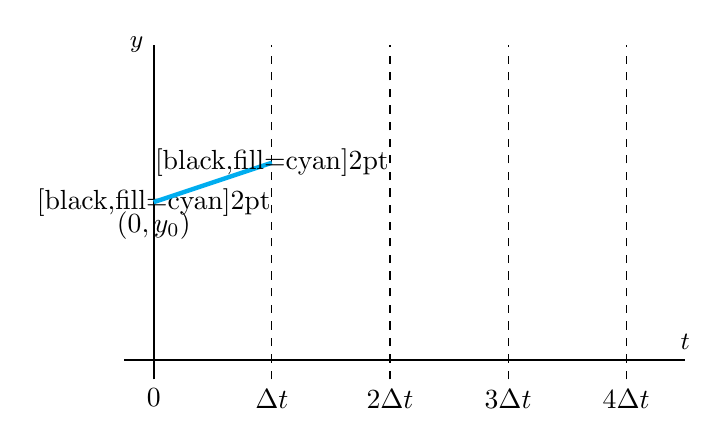
\begin{tikzpicture}[xscale=1.5]%,yscale=0.35]
		\draw[thick,-{\seta}] (-0.25,0) -- (4.5,0) node[above] {\small $t$};
		\draw[thick,-{\seta}] (0,-0.25) -- (0,4) node[left] {\small $y$};
		\foreach \t in {2,...,4} {
			\draw[dashed] (\t,-0.25) -- (\t,4);
			\draw[] (\t,-0.25) node[below] {$\t \Delta t$};
		}
		\draw[] (0,-0.25) node[below] {$0$};	
		\draw[dashed] (1,-0.25) -- (1,4);
		\draw[] (1,-0.25) node[below] {$\Delta t$};	
		\draw[] (0,2) node{\tikzcircle[black,fill=cyan]{2pt}};
		\draw[] (0,2) node[below] {$(0,y_0)$};
	%	\draw[ultra thick, lightblue] (5,2) node {\tikzcircle[black,fill=magenta]{2pt}}-- (3,6) node {\tikzcircle[black,fill=navy]{2pt}};
		\draw[ultra thick, cyan,-{\setam}] (0,2) -- (1,2.5);
		\draw[] (1,2.5) node{\tikzcircle[black,fill=cyan]{2pt}};
	\end{tikzpicture}
\end{center}

This way we find our second point \quad {\color{cyan} $(\Delta t,y_1)$} \quad where:
$$
\frac{y_1 - y_0}{\Delta t} = \text{ slope of the arrow }= f(0,y_0)
\quad \Rightarrow \quad
	y_1 = y_0 + f(0,y_0) \Delta t $$

We continue in this way to find more points \quad {\color{cyan} $(t_i, y_i)$}:
\begin{center}
	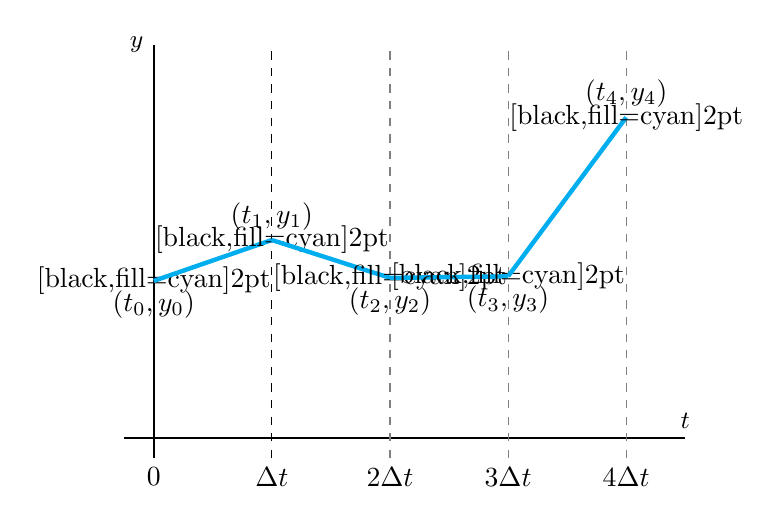
\begin{tikzpicture}[xscale=1.5]%,yscale=0.35]
		\draw[thick,-{\seta}] (-0.25,0) -- (4.5,0) node[above] {\small $t$};
		\draw[thick,-{\seta}] (0,-0.25) -- (0,5) node[left] {\small $y$};
		\foreach \t in {2,...,4} {
			\draw[dashed, gray] (\t,-0.25) -- (\t,5);
			\draw[] (\t,-0.25) node[below] {$\t \Delta t$};
		}
		\draw[] (0,-0.25) node[below] {$0$};	
		\draw[dashed] (1,-0.25) -- (1,5);
		\draw[] (1,-0.25) node[below] {$ \Delta t$};	
		\draw[] (0,2) node{\tikzcircle[black,fill=cyan]{2pt}};
		\draw[] (0,2) node[below] {$(t_0,y_0)$};
		\foreach \t in {1,...,4} {
			\draw[ultra thick, cyan,-{\setam}] ({\t-1},{2.25+(\t-2)^3/4-(\t-1)^2/2+(\t-1)/1.3}) -- ({\t},{2.25+(\t-1)^3/4-\t^2/2+\t/1.3});
			\draw[] (\t,{2.25+(\t-1)^3/4-\t^2/2+\t/1.3}) node{\tikzcircle[black,fill=cyan]{2pt}};
		}
		\foreach \t in {1,4} {
			\draw[] (\t,{2.25+(\t-1)^3/4-\t^2/2+\t/1.3}) node[above] {$(t_{\t},y_{\t})$};	
		}
		\foreach \t in {2,3} {
			\draw[] (\t,{2.25+(\t-1)^3/4-\t^2/2+\t/1.3}) node[below] {$(t_{\t},y_{\t})$};	
		}

	\end{tikzpicture}
\end{center}


\begin{definition}[Euler's Method]
	Let $y'(t) = f(t,y)$ be a first-order differential equation. 
	The \emph{Euler approximation} to the initial value problem $y'(t)=(f(t,y)$ and $y(t_0)=y_0$ with step size $\Delta t$ is the sequence of points $(t_i,y_i)$ given by $(t_0,y_0)$ if $i=0$ and 
	\begin{itemize}
		\item $t_i = t_{i-1}+\Delta t$
		\item $y_i = y_{i-1} +  f\big(t_{i-1},y_{i-1}\big) \Delta t$.
	\end{itemize}
	
	The method used to generate $(t_i,y_i)$ is called \emph{Euler's Method}.
\end{definition}


\begin{example}
Consider the initial-value problem
$$
\begin{cases}
y'(t) = \sin(y)+t \\
y(-3)=2
\end{cases}
$$

\begin{minipage}{.65\textwidth}
Then, we can follow Euler's Method with $h=0.5$ to obtain:
\begin{itemize}
	\item $y_0=2$
	\item $y_1 = 2 + \frac12 \big(\sin(2) -3\big) \approx 0.95$
	\item $y_2 = 0.95 + \frac12 \big(\sin(0.95) -2.5\big) \approx 0.1$
	\item $y_3 = 0.1 + \frac12 \big(\sin(0.1) -2\big) \approx -0.85$
\end{itemize}

%\begin{center}
%%	\begin{figure}[hbtp]
%	\includegraphics*[width=200pt]{images/module10-Euler.pdf}
%%	\caption{Graph of the Euler approximation and the slope field for the differential equation using desmos.}
%%	\end{figure}
%\end{center}
	
\begin{minipage}{220pt}
Here is the link to the desmos graph: 
\begin{itemize}
	\item \href{https://www.desmos.com/calculator/kkgj5jhggd}{https://www.desmos.com/calculator/kkgj5jhggd} %\hfill \qrcode{https://www.desmos.com/calculator/kkgj5jhggd}
\end{itemize}
\end{minipage}
\hfill
\begin{minipage}{55pt}
	\qrcode{https://www.desmos.com/calculator/kkgj5jhggd}
\end{minipage}
\end{minipage}
\hfill
\begin{minipage}{150pt}
	\includegraphics*[width=150pt]{images/module10-Euler-small.pdf}
\end{minipage}	

\end{example}


\begin{video}
\begin{itemize}
	\item \qrvideo{https://youtu.be/q87L9R9v274}
	\item \qrvideo{https://youtu.be/g3Xw1r7QGOE}
	\item Euler's Method helping to take a person to the Moon \hfill \qrcode{https://youtu.be/v-pbGAts_Fg}
\end{itemize}	
\end{video}






	\begin{exercises}
	
	\begin{problist}
	
	\prob \label{approx:comp}For the following initial-value problems, approximate their solution with different values of $\Delta t$ and compare with their exact solutions. 
	\begin{enumerate}
		\item $y'=-y+5+t$, $y(0) = 4,5,6$
		\item $y'=y+5-t$, $y(0) = -4$
		\item $y'=(t-y)\sin(y)$, $y(0)=-1$
		\item $\displaystyle y'=\frac{y+3t}{1+t^2}$, $y(0)=-1,1$
	\end{enumerate}
	
	\textbf{Hint. } Write a computer program that does the approximation for you.
	
	
	\prob Consider the differential equation
	$$ y'=-\frac{x}{y}.$$
	\begin{enumerate}
		\item Sketch a slope field for this differential equation.
		\item Use Euler's Method to approximate the solution for some values of $\Delta x$ and for some initial conditions.
		\item Does Euler Method do a good job approximating the solution?
	\end{enumerate}
	
	\begin{annotation}
	\begin{Goals}
		There is a singularity at $y=0$, so the method will behave erratically when it goes across that line.
			\href{https://www.desmos.com/calculator/5swjyrxvtr}{https://www.desmos.com/calculator/5swjyrxvtr} \hfill \qrcode{https://www.desmos.com/calculator/5swjyrxvtr}
	\end{Goals}
	\end{annotation}
	
	
	
	
	\prob In this module, we derived Euler's Method. One of the main steps was obtaining the equation
	$$\frac{y_1-y_0}{\Delta t} = \text{slope of the arrow}.$$
	
	In Euler's Method, we used the slope at the beginning of the arrow. We can derive a new Method where we use the slope at the end of the arrow. 
	
	\begin{enumerate}
		\item Find a formula and the algorithm for this new method.
		\item Use this method with to approximate the solution of $y'=-y+5+t$, $y(0) = 4,5,6$ and compare the results with your results from question \ref{approx:comp}.
		\item Which of these two methods gives a better approximation?
		\item In your opinion, which of these two methods is better? Why?
	\end{enumerate}
	
	
	
	
	
	
	
	
	
	
	
	\prob Consider an initial-value problem with solution $y(t)$. If we want to find an approximation for $t \in [0,T]$, we define the error of the approximation $\{y^{\Delta t}_i\}$ by
	\begin{equation}\tag{E}\label{error} 
		E(\Delta t) = \big| y(T) - y^{\Delta t}_N \big|,
	\end{equation}
	where $T = N \Delta t$.
	
	\begin{enumerate}
		\item For the initial-value problems from the previous question, study what happens when the value of $\Delta t$ decreases.
		\item What do you expect to happen as $\Delta t$ converges to $0$?
		\item Estimate how fast Euler's method converges. Find a value of $p$ such that
			$$ E(\Delta t) \leq C (\Delta t)^p,$$
		where the constant $C$ changes for each ODE, but doesn't change if you keep the same ODE but change only the value of $\Delta t$.
%		\item In fact, when using Euler's method on a computer, there are more approximations that are subtler. For example, the computer approximates every number that you write and it also approximates every operation that the method needs. This means that the real error of the approximation 
	\end{enumerate}
	

	\prob Using Euler's Method with a step size of $\Delta t = 0.05$, and keeping only three digits throughout your computations, determine the approximations at $T=0.2, 0.3, 0.4$ for each of the following initial-value problems.
	\begin{enumerate}
		\item $y'=-y+5+t$, $y(0) = 4$
		\item $y'=y+5-t$, $y(0) = -4$
	\end{enumerate}
	Compare the results with what you obtained for problem \ref{approx:comp}. Where do the differences come from?
	
	\prob Round-off errors become important when the value of $N$ is very large, which happens if we want a very accurate approximation. This means that the actual error \eqref{error} of the approximation has two components:
	$$ E(\Delta t) = f(\Delta t) + g(\Delta t), $$
	where
	\begin{itemize}
		\item $\displaystyle \lim_{\Delta t \to 0^+} f(\Delta t) = 0$ \hfill (approximation error)
		\item $\displaystyle \lim_{\Delta t \to \infty} f(\Delta t) = \infty$ \hfill (approximation error)
		\item $\displaystyle \lim_{\Delta t \to 0^+} g(\Delta t) = \infty$ \hfill (round-off error)
		\item $\displaystyle \lim_{\Delta t \to \infty} f(\Delta t) = 0$ \hfill (round-off error)
	\end{itemize}
	
	Answer the following questions and justify your answers based on these ideas.
	\begin{enumerate}
		\item Justify why the four limits above make sense.
		\item Does the approximation converge to the solution as $\Delta t \to 0$?
		\item Is there an optimal $\Delta t$ that gives the best possible approximation?
	\end{enumerate}
	
	

	
	
	\end{problist}
\end{exercises}
\end{module}



\begin{lesson}
	\Title{Approximating Solutions}

%	\Heading{Objectives}
%%	\begin{itemize}
%%		\item The second step in Mathematical modelling is to construct a representation of how the team will be attempting to solve the problem.
%%		\item Create a mind map of the problem. This is a structured way to brainstorm possible solutions and their requirements.
%%	\end{itemize}
%	
%	\Heading{Motivation} 
%
%\begin{annotation}
%	\begin{goals}
%	\Goal{Extra Reading}
%	Math Modelling: Getting started and getting solutions, Bliss-Fowler-Galluzzo
%	
%	\hfill \qrcode{https://m3challenge.siam.org/resources/modeling-handbook}	
%	\end{goals}
%\end{annotation}
%	\Heading{Extra Reading} \href{https://m3challenge.siam.org/resources/modeling-handbook}{Math Modelling: Getting started and getting solutions, Bliss-Fowler-Galluzzo}
%
\end{lesson}




\newpage

\question
	Consider the differential equation
	$$ y' = y - 2 .$$
	
\begin{parts}
	\item Use Euler's Method to find an approximation of the solution of this differential equation that passes through the point $(0,3)$.
	\item Find the solution of the differential equation with the same initial condition.

	\item Use Euler's Method to find an approximation of the solution of this differential equation that passes through the point $(0,1)$.
	\item Find the solution of the differential equation with the same initial condition.

	\item Compare the approximations with the actual solutions. Is there a property of the Euler's Method that you can infer?
	\item Explain in words why the Method satisfies that property.
	

\end{parts}

\begin{annotation}
	\begin{Goals}
		The goal is to have student's recognize that the Euler approximation ``curves slower'' than the actual solution.
		
		Students can explain in words why that is the case using the way the approximations are generated.
	\end{Goals}
\end{annotation}


\bookonlynewpage



\question
	Which differential equations will be approximated perfectly using Euler's Method?

\begin{annotation}
	\begin{Goals}
		The question is purposefully ambiguous.
		What do we mean by approximated perfectly?
		
		Ex: The IVP $y'=$ sign$(t)$ (assuming sign$(0)=1$) with $y(-5)=5$ has solution $y = |t|$ and it is captured with Euler's method if $\Delta t=\frac5k$ for any $k\in\mathbb{N}$. \\
		
		Once students discuss, they'll find ODE's of the form $y'= c$ for any constant. 
		
		Prompt them to find other types. Show them the example above only after they tried for a bit. 
		Then, let them revise their Conjecture.  \\
		
		Ex 2: $y'=f(y+t)$ with $y(0)=0$ and $f(z) = \lfloor z \rfloor$ is approximated perfectly if $\Delta t = 1$, but not if $\Delta t$ takes any other value.
		
	\end{Goals}
\end{annotation}








%\bookonlynewpage







%%%%%%%%%%%%%%%%%%%%%%%%%%%%%%%%%%%%%%%%%%%%%%%%%%%%%%%%%%%%%%%%%%%%%%%%
%
%		Chapter 3 -
%
%%%%%%%%%%%%%%%%%%%%%%%%%%%%%%%%%%%%%%%%%%%%%%%%%%%%%%%%%%%%%%%%%%%%%%%%
%
%
%\begin{topic}[First-Order Models]
%
%\end{topic}
%
%

%%%%%%%%%%%%%%%%%%%%%%%%%%%%%%%%%%%%%%%%%%%%%%%%%%%%%%%%%%%%%%%%%%%%%%%%
%		Modelling with ODEs


\begin{module}{Modelling with Differential Equations}
	%\Title{Slope Fields}
	\label{model-odes}

	In this module you will learn
\begin{itemize}
	\item how to start modelling a physical phenomenon into a differential equation
\end{itemize}

\hfill \\


We started by studying some mathematical modelling in chapter 1. Then, we just used mathematical tools that we learned before. 

We now want to focus on mathematical models that arise from physical applications. These will often take the form of one or more differential equations.

The modelling of the situation will develop in a similar way.


\paragraph{\emph{Step 1.}} Defining the problem \\

As before, we should start by thinking about what our ultimate goal is. 
Once we settle on a goal, we define it as the function we want to study.

\begin{example}

\begin{minipage}{.7\textwidth}
In this module, we are going to think about the catapult problem from Module 9 - Slope Fields. \\

A catapult throws a projectile into the air.

Our goal is to track the height (in metres) of the projectile from the ground.

This means that we have a goal: to find the height of the projectile at every moment in time after it is launched.
\end{minipage}\hfill
\begin{minipage}{100pt}
	\includegraphics*[width=100pt]{images/module9-catapult.pdf}	
\end{minipage}
\hfill \\[10pt]

This means that we define
\begin{itemize}
	\item $y(t) = $ height of the projectile, in metres, $t$ seconds after it was launched from the catapult.
\end{itemize}

\end{example}

\hfill \\

\paragraph{\emph{Step 2.}} Building a mind map \\

A mind map will help us identify the notions that we want to include in our model.


\begin{example}

In the catapult example, since we decided to study the projectile's height, we need to find everything that affects its height.

\begin{center}
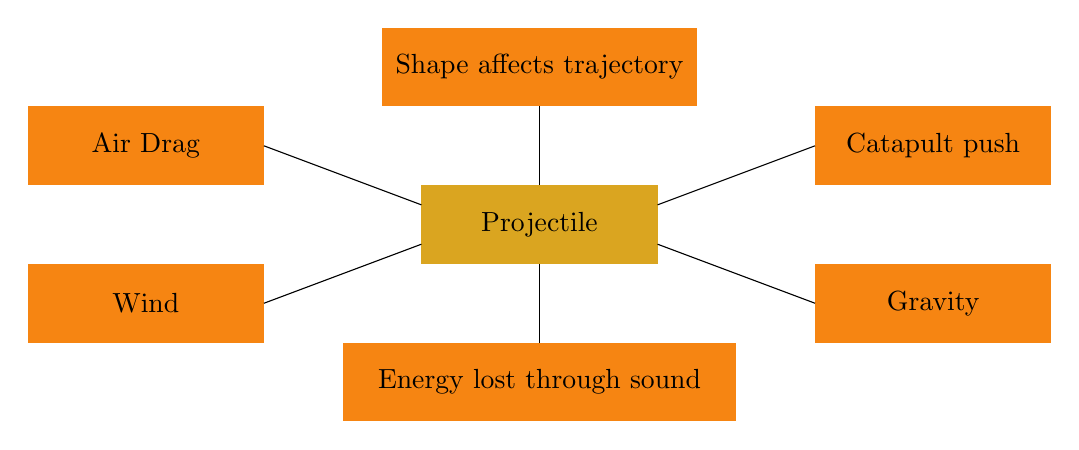
\begin{tikzpicture}
	\fill[color=Goldenrod] (0,0) rectangle (3,1) node[pos=.5] {\color{black}Projectile};
	\fill[color=BurntOrange] (5,1) rectangle (8,2) node[pos=.5] {\color{black}Catapult push};
	\fill[color=BurntOrange] (5,-1) rectangle (8,0) node[pos=.5] {\color{black}Gravity};
	\fill[color=BurntOrange] (-5,1) rectangle (-2,2) node[pos=.5] {\color{black}Air Drag};
	\fill[color=BurntOrange] (-5,-1) rectangle (-2,0) node[pos=.5] {\color{black}Wind};
	\fill[color=BurntOrange] (-1,-2) rectangle (4,-1) node[pos=.5] {\color{black}Energy lost through sound};
	\fill[color=BurntOrange] (-0.5,2) rectangle (3.5,3) node[pos=.5] {\color{black}Shape affects trajectory};
	\draw (3,0.75) -- (5,1.5);
	\draw (3,0.25) -- (5,-0.5);
	\draw (0,0.75) -- (-2,1.5);
	\draw (0,0.25) -- (-2,-0.5);
	\draw (1.5,0) -- (1.5,-1);
	\draw (1.5,1) -- (1.5,2);
\end{tikzpicture}
\end{center}

We can include more layers to these topics if we want.

\end{example}


\hfill \\

\paragraph{\emph{Step 3.}} Make assumptions \\

This is a fundamental step in any modelling endeavour. The real world is too complicated, so we make assumptions that simplify our model.

This has two main consequences:
\begin{enumerate}
	\item It makes our model simpler and easier to study;
	\item It creates constraints on our model: it is only valid under certain conditions.
\end{enumerate}

\begin{example}

Let us discuss the topics included in the mind map above:
\begin{itemize}
	\item Catapult Push -- the catapult pushes on the projectile for a small period of time when $t<0$. If we are considering only $t\geq 0$, then this will likely provide us with some starting conditions for the projectile
	\item Gravity -- The height of the projectile is affected by gravity. We have a choice to make:
	\begin{itemize}
		\item assume that the Earth is flat and gravity is constantly accelerating the projectile downwards;
		\item assume that the Earth is spherical and gravity is constantly accelerating the projectile towards the centre of the Earth;
		\item assume that the Earth is spherical and gravity is a force accelerating the projectile towards the centre of the Earth with a magnitude that decreases with the square of the distance to the centre of the Earth
		\item or other more complicated and more accurate models.
	\end{itemize}
	
	\item Air Drag -- air is making it hard for the projectile to move forward. We have another choice to make:
	\begin{itemize}
		\item assume that the air drag is a force that accelerates the projectile in the direction opposite to its movement and with magnitude proportional to its speed;
		\item assume that the air drag is a force that accelerates the projectile in the direction opposite to its movement and with magnitude proportional to the square of its speed;
		\item or other more complicated and more accurate models.
	\end{itemize}
\end{itemize}
	
I will leave it to you to think about the remaining three topics in the mind map. \\


We now need to make a decision about what to assume. \\

To keep this model simple, let us assume the following:
\begin{enumerate}
	\item The projectile's height will stay within a small range: $y(t) \in [0,100]$. Is this reasonable for a catapult?

		This means that we can consider the first of the gravitational models above: define gravitational acceleration as a constant $-g$.
		
	\item The projectile will not move very fast, so we can approximate the air drag to be directly proportional to the speed: define air drag acceleration as $\pm \gamma v$, where $\gamma>0$ is a constant that depends on the projectile and $v$ is the velocity of the projectile. Which sign should we have?

	\item Again, the projectile will not move very fast, so we can approximate the air drag to use only the vertical speed of the projectile: define air drag acceleration as $\pm \gamma v_y$, where $\gamma>0$ is a constant that depends on the projectile and $v_y$ is the vertical velocity of the projectile. Which sign should we have?

	\item The shape of the projectile will affect air drag in the form of the constant $\gamma>0$.

	\item Assume that for a medieval catapult (as in the drawing above), the other components are negligible.

\end{enumerate}

We come out of this step with some conditions for the validity of our model and some new constants and terms to use in our model.

\end{example}

\hfill \\

\paragraph{\emph{Step 4.}} Construct a model \\

This is the part where we put together the last three steps into one (or a system of) differential equations.

This should not be a difficult part if the last three steps were completed carefully.

\begin{example}

Summary of Steps 1--3:
\begin{itemize}
	\item \textbf{Goal:} study $y(t) = $ height of a projectile in metres, $t$ seconds after being released from a catapult
	\item \textbf{Forces:}
	\begin{itemize}
		\item Gravity: constant acceleration $-g$
		\item Air Drag: acceleration $\pm \gamma y'(t)$
	\end{itemize}
	\item \textbf{Conditions:}
	\begin{itemize}
		\item $y(t) \in [0,100]$
		\item Air drag should really by quadratic, but in this example we will consider this as an academic case.
	\end{itemize}
\end{itemize}

So the model we end up is:
$$
F_y = \substack{\text{vertical component}\\\text{of force}} = -g \pm \gamma y'.
$$

Now we bring a little bit of a Physics class into here: Newton's 2$^{\rm nd}$ Law states that \quad $F = m a$ \quad, so we obtain the model
$$m y''(t) =  -g \pm \gamma y'(t).$$
\end{example}



\paragraph{\emph{Step 5.}} Model Assessment

We just found a differential equation (model) for our situation. It is now time to test it to make sure that it behaves correctly.

For this step, we need to obtain a solution of the differential equation, either by solving it mathematically and finding a formula for the solution, or by approximating the solution numerically (see Module \ref{NumericalMethods}).

Then we need to check if the differential in one of several ways:
\begin{itemize}
	\item We can test it empirically: make an experiment and compare the results of the experiment with the results of the model
	\item We can test it mathematically: change the parameters and the initial conditions to make sure that we know how the model should behave and test some qualitative aspects of the model
\end{itemize}

\begin{important}
Even if the model passes all the tests, it might still not be correct.

Also, if it fails one test, it might mean that the model is incorrect, or that it has some limitations that are more subtle and we hadn't thought about them.	
\end{important}

\begin{example}
We have found the following model:
\begin{itemize}
	\item $y(t) = $ height of a projectile in metres, $t$ seconds after being released from a catapult
	\item It satisfies:
		$$m y''(t) =  -g + \gamma y'(t).$$
	(note that I chose the $+$ sign for the air drag component)

	\item Constraints:
	\begin{itemize}
		\item $y(t) \in [0,100]$;
		\item $\gamma >0$ is the drag constant: more air drag for larger values of $\gamma$;
	\end{itemize}
\end{itemize}	

This differential equation tells us what the second derivative, $y''(t)$, of $y(t)$ is given the first derivative $y'(t)$.
This means that to start solving the problem, we need to know what the initial values for $y'(t)$ and $y(t)$ are.

Need to know the starting conditions:
\begin{itemize}
	\item $y(t_0) = y_0$;
	\item $y'(t_0) = v_0$.
\end{itemize}

For this example, consider a situation where:
\begin{itemize}
	\item $g, \gamma >0$ can take any value.
	\item $y(0) = 0$;
	\item $y'(0) = g/\gamma > 0$;
\end{itemize}

The projectile is being catapulted from the ground with a positive velocity, so we expect it to go up for a while and then come back down to the ground.

What happens is 
$$
y''(0) = -g + \gamma y'(0) = 0,
$$
so the initial acceleration is 0, which means that the velocity is not changing.

The result is a function with constant velocity equal to its initial velocity:
\begin{itemize}
	\item $y(t) = \frac{g}{\gamma}t.$
\end{itemize}

This means that the height of the projectile keeps increasing, so the \emph{projectile never falls back to the ground}! \\

This means that there is a problem with our differential equation:
\begin{itemize}
	\item Is the model incorrect? 
	\item Is there a limitation on the initial velocity that we were not aware of?
\end{itemize}
\hfil

We must check our process again and correct it.
\end{example}




\paragraph{\emph{Step 6.}} Putting it all together in a report

We're not going to elaborate much on this step. For more on the subject, please check Module \ref{report}.





\begin{video}
\begin{itemize}
	\item \href{https://youtu.be/njg8xwMviGQ}{https://youtu.be/njg8xwMviGQ} \hfill \qrcode{https://youtu.be/njg8xwMviGQ}
	\item \href{https://youtu.be/nKDsJB8iwb0}{https://youtu.be/nKDsJB8iwb0} \hfill \qrcode{https://youtu.be/nKDsJB8iwb0}
\end{itemize}	
\end{video}


	\begin{exercises}
		% Topics:
		% 
	\begin{center}
		\includegraphics*[width=175pt]{images/module11-lake.pdf}
	\end{center}
	\begin{problist}
	\prob Model the pollution in a lake where water flows in and out at the same rate and incoming water is polluted with $2+\sin(2t)$ kg/L of pollutant, where $t$ is measured in years.
	
		
	\prob Construct a model for a population with a rate of growth proportional to its current size.
	
	\prob Find a model for a population that grows proportionally to its current size but with a variable proportion constant. This variable proportion constant should guarantee the following properties for the population:
	\begin{itemize}
		\item If the population is too large, then it should decrease;
		\item If the population is small, then it should increase.
	\end{itemize}
		
	
	\prob Improve the previous model by considering also a \emph{survivability threshold}: if the population is below this value, it should decrease and eventually become extinct.
		
	
	\prob Consider two competing populations, like cheetahs ($c(t)$) and lions ($\ell(t)$): two populations that do not hunt each other, but compete for the same food (prey). Create a model for these two populations that captures how the competition for food affects them.
	
	{\bf Hint. } It might be helpful to think about how one population would grow in the absence of the other; and how one population is affected by the competition of the other.

	\begin{center}
			\includegraphics*[width=150pt]{images/module11-stadium.pdf}
	\end{center}
		
	\prob People are in a stadium watching cricket match. When the match is over, people leave the stadium. 
	
	\begin{enumerate}
	\item Model the way people leave the stadium.
	
	To help you with this task, use the fact that in this situation, people behave like a fluid according to Torricelli's Law:
	
		\begin{center}
		\framebox{
		\begin{minipage}{6cm}
		\begin{center}
		The area of the region occupied by the fans decreases proportionally to the square root of the radius and also proportionally to the size of the exit.
		\end{center}
		\end{minipage}}
		\end{center}

	\item How do the parameters $\theta$ and $\alpha$ affect the total time it will take for the stadium to empty?
	\end{enumerate}
	
	\begin{center}
		\includegraphics*[width=150pt]{images/module11-pool.pdf}
	\end{center}
	
	
	\prob Consider the pool in the figure. The goal is to track the amount of chlorine in the water for one Summer month. At the beginning of the month, the pool is full and contains 150g of chlorine uniformly mixed in the water. Consider evaporation and rain. To make the model simpler, assume that water evaporates with the chlorine.
	
	
	
	\prob After solving the core exercise \ref{pendulum} below, we find a property of this model. 
	\begin{enumerate}
		\item The constants $g$ and $L$ (length of the string) appear only has $\frac{g}{L}$. What does this imply?
		\item We are sending a mission to the Moon and we need to know how a 1m long pendulum behaves on the Moon. To test it, we need to build on Earth a pendulum that behaves in the same way. How long should the length of the string be on Earth?
	\end{enumerate}
	

	\prob After solving the core exercise \ref{pendulum} below, construct a model for the same problem considering string tension.
	\begin{enumerate}
		\item Show that you obtain the same model that you get while disregarding tension.
		\item Explain why this makes sense.
	\end{enumerate}
	
	\begin{center}
		\includegraphics*[width=150pt]{images/module11-ant_tunnel.pdf}
	\end{center}
	
	\prob 	An ant queen, known affectionately as Aunty Ant, is commissioning a construction assessment
	for a new tunnel.  Aunty Ant's worker ants only know one way to construct a tunnel: they grab some dirt in their pincers,
	walk the dirt out of the tunnel, deposit it, and then return to grab more dirt.
	
	Prepare a report which uses differential equations to address the following construction scenarios.  Include a
	description of how you modelled the scenario and a graph of tunnel-length vs.~worktime.
	Also make sure to define any variables and constants you are using.

	\begin{enumerate}
		\item One tireless worker is assigned dig the tunnel.  The worker walks the same speed
			whether she is carrying dirt or not.
		\item One tireless worker is assigned to dig the tunnel, but she can walk twice as fast
			when she is not carrying dirt as when she is carrying dirt.
		\item Aunty Ant really wants the tunnel to progress linearly after the first
			day of construction (that is, the graph of tunnel-depth vs.~time after
			the first day should be a straight line).  She will give you full control over
			how many workers are devoted to the tunnel at any given time.
		\item (Optional) A single ant is assigned to dig the tunnel, but she gets fatigued
			the farther she walks.  Her speed after walking a total distance of $k$ units is $1/k$.

	\end{enumerate}


	\prob 	The alien world of Robotron is inhabited by billions of tiny nanobots.  These nanobots
	all share a common source of power, and their speed is directly proportional to the
	total amount of energy shared among all the nanobots. 

	One day the nanobots decide to beam their energy into space.  They all form lines,
	march to the edge of their colony, and send a tiny portion of their shared energy into
	space.  Since the nanobots are very polite, after an individual nanobot has sent its energy
	into space, it moves aside and lets the next nanobot take a turn.

	\begin{enumerate}
		\item Suppose the nanobots live in a tube with an opening at only one end.  Come
			up with a differential equation to model the amount of energy left in the nanobot
			colony over time.
		\item How does your model change if the nanobots live in a disk where energy can be launched
			from anywhere on the perimeter?  What about a sphere?
		\item Newton's law of cooling states that the rate of change of temperature of an object is
			proportional to the difference between the object's temperature and the ambient (outside)
			temperature.  Does this law relate to your model for the nanobots?  If so, how?
	\end{enumerate}

	
	\end{problist}
\end{exercises}

\end{module}



\begin{lesson}
	\Title{Modelling with Differential Equations}

%	\Heading{Objectives}
%	\begin{itemize}
%		\item The second step in Mathematical modelling is to construct a representation of how the team will be attempting to solve the problem.
%		\item Create a mind map of the problem. This is a structured way to brainstorm possible solutions and their requirements.
%	\end{itemize}
%	
%	\Heading{Motivation} 
%
%\begin{annotation}
%	\begin{goals}
%	\Goal{Extra Reading}
%	Math Modelling: Getting started and getting solutions, Bliss-Fowler-Galluzzo
%	
%	\hfill \qrcode{https://m3challenge.siam.org/resources/modeling-handbook}	
%	\end{goals}
%\end{annotation}
%	\Heading{Extra Reading} \href{https://m3challenge.siam.org/resources/modeling-handbook}{Math Modelling: Getting started and getting solutions, Bliss-Fowler-Galluzzo}

\end{lesson}




\newpage


\begin{annotation}
	\begin{goals}
	\Goal{Pendulum and Rumours}
		This should take 2 lectures.
		
		Lecture 1. Focus on Pendulum problem. Students should finish it at home.
		
		
		Lecture 2. Rumour problem is more open-ended. 
		
		Students should follow the structure from chapter 1 to think about this problem.
	\end{goals}
\end{annotation}
		
		
		
\question \label{pendulum}
	A pendulum is swinging side to side. We want to model its movement.

\begin{minipage}{.7\textwidth}
\begin{parts}
	\item Define the problem. Which function(s) do we want to find in the end?
	\item Build a mind map.
	\item Make assumptions. Remember to use your mind map to help structure the problem.
	\item Construct a model. You should end up with one (or more) differential equations. 
	
	Remember that there are some Physics principles that can help you (e.g. Newton's 2$^{\rm nd}$ Law, Conservation of Energy, Linear Momentum, and Angular Momentum, Rate of Change is Rate in $-$ Rate out).
	\item Assess your model:
	\begin{enumerate}
		\item Find one test that your model passes.
		\item Find one test that your model fails.
	\end{enumerate}
	
\end{parts}
\end{minipage}\hfill
\begin{minipage}{100pt}
	\includegraphics*[width=100pt]{images/module11-pendulum.pdf}	
\end{minipage}







\begin{annotation}
	\begin{goals}
		Students will mostly likely identify the goal as finding the position of the ball $\vec{r}(t) = \big( x(t) , y(t) \big)$. That's fine!
		
		Later, in Step 3, try to guide the students to recognize the following:
		\begin{itemize}
			\item Rope is massless (negligible)
			\item Rope doesn't bend (negligible)
			\item So can assume that the rope is rigid. How does that affect the position of the ball?
			\item No friction (negligible)
			\item \textbf{Important:} Students always focus on string tension. One can consider it, but it all cancels out. It's one of the exercises of the module (above). For the lecture, don't consider tension.
		\end{itemize}
		
		Then on Step 4, guide students to recognize that they actually only need to find a model for the angle, because the position of the ball really only depends on the angle $\theta(t): \vec{r}\big(\theta(t)\big)$
				
	\end{goals}
\end{annotation}







\bookonlynewpage

\hfill



\bookonlynewpage

\question \label{rumour} Model the spreading of a rumour through the students of a school.






%%%%%%%%%%%%%%%%%%%%%%%%%%%%%%%%%%%%%%%%%%%%%%%%%%%%%%%%%%%%%%%%%%%%%%%%
%		Solvable Types of ODEs: Separable, First-Order Linear, Exact (?)


\begin{module}{Solvable Types of ODEs}
	%\Title{Separable ODEs}

	\label{model-odes}

	In this module you will learn
\begin{itemize}
	\item to identify specific types of differential equations that can be solved rigorously
	\item how to solve these types of differential equations
\end{itemize}

\hfill \\

We just learned how to model a situation and end up with a differential equation.
We will now focus on solving differential equations. 

There are a few different techniques that depend on the differential equation. 

\hfill

\begin{submodule}{Separable Differential Equations}

\begin{definition}[Separable ODE]
A differential equation is called \emph{separable} if it has the form
$$
g(y) y'(t) = h(t),
$$
that is if we can separate all the $y$'s into the left-hand side and the all the $t$'s into the right-hand side of the equation. Observe that the $y$'s on the left hand side must all be multiplied by $y'(t)$. 
\end{definition}


\subparagraph{\textcolor{cyan}{Method of solution. }} The idea to solve this type of DEs is simple:
\begin{enumerate}[label={\bf \arabic*. } ]
\item Integrate both sides with respect to $t$:
$$
\int g(y) y'(t) \, dt = \int h(t) \, dt
$$

\item Change variables on the left-hand side to $u = y(t)$, so $du = y'(t) dt$ and we get
$$
\int g(u) \, du = \int h(t) \, dt.
$$

\item Solve both integrals and we obtain a solution, usually in implicit form:
$$
G(u) = H(t) + C.
$$

\item To finish, recall that $u=y(t)$, so we obtain
$$
G\big(y(t)\big) = H(t) + C.
$$
\end{enumerate}

\begin{important}
	Observe that the solution is given in implicit form. In general, when using this technique, the solution $y(t)$ will be given in implicit form, so there is still some work ahead to find an explicit formula for $y(t)$.	
\end{important}



\def\arcsinh{\rm arcsinh\ }
\begin{example}
The shape $y(x)$ of a free falling chain under its own weight, called a catenary, satisfies the differential equation:
$$
y''(x) = \frac1a \sqrt{1+\big(y'(x)\big)^2}.
$$

It doesn't seem to be a \textbf{\color{Red!70!black}separable equation}, but if we can define $z(x) = y'(x)$, which satisfies
$$
z'(x) = \frac1a \sqrt{1+\big(z(x)\big)^2}
\qquad \Leftrightarrow \qquad \frac{1}{\sqrt{1+\big(z(x)\big)^2}} z'(x) = \frac1a.
$$

This is now clearly in the form of a \emph{\color{Red!70!black}separable ODE}. \\

We can solve it using the method described above: we need to solve
$$
\int \frac{1}{\sqrt{1+z^2}}\,dz \quad = \quad \int \frac1a \,dx \quad = \quad \frac{x}{a} + C_1
$$
The integral on the left can be solved using a hyperbolic substitution $z = \sinh u$:
$$
\int \frac{1}{\sqrt{1+z^2}}\,dz = \int 1 \, du = u = \arcsinh z.
$$
This means that the solution satisfies
$$
\arcsinh z = \frac{x}{a} + C_1 
\qquad \Leftrightarrow \qquad z = \sinh \left(\frac{x}{a} + C_1 \right).
$$

Now recall that $z(x) = y'(x)$, so we need to integrate $z(x)$ to obtain the catenary curve $y(x)$:
$$
y(x) = \int z(x) \, dx = a \cosh \left(\frac{x}{a} + C_1\right) + C_2.
$$

To find $C_1$ and $C_2$, we use the fact that $y'(0)=0$:
$$
y(x) = a \cosh \frac{x}{a}  + C_2.
$$
(the constant $C_2$ moves the curve up or down, so it doesn't change the shape).
\end{example}


\begin{video}
\begin{itemize}
	\item \href{https://youtu.be/txtFH89HwOA}{https://youtu.be/txtFH89HwOA} \hfill \qrcode{https://youtu.be/txtFH89HwOA}
	\item \href{https://youtu.be/8xG_Xg6X2MQ}{https://youtu.be/8xG\_Xg6X2MQ} \hfill \qrcode{https://youtu.be/8xG_Xg6X2MQ}
	\item \href{https://youtu.be/ZE1Agfkhr28}{https://youtu.be/ZE1Agfkhr28} \hfill \qrcode{https://youtu.be/ZE1Agfkhr28}
\end{itemize}	
\end{video}

\end{submodule}

\hfill \\

\begin{submodule}{First-Order Linear Differential Equations}

\begin{definition}[First-Order Linear ODE]
A differential equation is called \emph{first-order linear} if it has the form
$$
y'(t) + p(t) y(t) = f(t),
$$
that is if we can separate all the $y$'s into the left-hand side and the all the $t$'s into the right-hand side of the equation. Observe that the $y$'s on the left hand side must all be multiplied by $y'(t)$. 
\end{definition}


The idea to solve this type of DEs is to transform it into the result of a product rule. \\


\begin{example}
Consider the following \textbf{\color{Red!70!black}first-order linear ODE}
$$
t^2 \frac{dy}{dt} + 2t y = \sin t.
$$

Observe that the left-hand side of the DE is the result of the product rule:
$$
\frac{d}{dt} \bigg[ t^2 y \bigg] = \sin t.
$$
So  we can integrate both sides with respect to $t$ to obtain
$$
t^2 y = - \cos t + C 
\quad \Leftrightarrow \quad y = -\frac{\cos t}{t^2} + \frac{C}{t^2}.
$$
\end{example}


Now let us look at another example, where the left-hand side of the ODE is not in the form of the result of a product rule, but can be transformed into one.


\begin{example}
Consider the \textbf{\color{Red!70!black}first-order linear ODE}
\begin{equation}\tag{$\star$}\label{eq:intfact_1}
\frac{dy}{dt} + \frac12 y = \frac13 e^{\frac t3}.
\end{equation}
%which passes through the point $(0,1)$.


Again, the ``trick'' is to look at this equation and realize that the left-hand side can look like the result of the product rule.
It's not obvious that this can be done (yet!), but if we multiply the whole ODE by the function
$$
e^{\frac{t}{2}},
$$
then we obtain
$$
e^{\frac t2} \frac{dy}{dt} + \frac12e^{\frac t2} y = \frac13 e^{\frac t2} e^{\frac t3}
$$
and now the left-hand side is the result of a product rule
$$
\frac{d}{dt}\left[e^{\frac t2} y \right] = \frac13e^{\frac 56 t}.
$$

We integrate both sides to obtain
$$
e^{\frac t2} y = \frac13 \frac65 e^{\frac56 t} + c
$$
thus
$$
y %= \frac25 e^{\frac56 t-\frac12t} + c e^{-\frac t2} 
	= \frac25 e^{\frac t3} + c e^{-\frac t2}.
$$

\end{example}


This last example required us to come up with a function to multiply the ODE so that it becomes of the right form: with a left-hand side that is the result of the product rule.

This function is called the \textbf{\color{cyan}integrating factor}.

Let us now see how we can find this function in more detail.


\begin{example}
Consider the same ODE \eqref{eq:intfact_1}:
\begin{equation}\tag{$\star$}
\frac{dy}{dt} + \frac12 y = \frac13 e^{\frac t3}.
\end{equation}

So we multiply both sides of the equation with an unknown function $\mu(t)$, called the \textbf{\color{cyan}integrating factor}:
\begin{equation}\tag{\#}\label{eq:intfactor2}
\mu(t) \frac{dy}{dt} + \frac12 \mu(t) y = \frac13 \mu(t) e^{\frac t3}.
\end{equation}

And we find which $\mu(t)$ makes the left-hand side equal to the product rule:
$$
\frac{d}{dt} \big[ \mu(t) y \big] 
	= \mu(t) \frac{dy}{dt} + \frac{d \mu(t)}{dt} y,
$$
and this needs to equal the left-hand side:
$$
\mu(t) \frac{dy}{dt} + \frac{d \mu(t)}{dt} y = \mu(t) \frac{dy}{dt} + \frac12 \mu(t) y
\qquad \Leftrightarrow \qquad
	\mu'(t) = \frac12 \mu(t).
$$

We now need to solve this equation for $\mu(t)$. Fortunately, this is a \textbf{\color{cyan}separable ODE}:
\begin{align*}
\mu'(t) = \frac12 \mu(t) \quad
	& \Leftrightarrow \quad \frac{\mu'(t)}{\mu(t)} = \frac12 \\
	& \Leftrightarrow \quad \ln |\mu(t)| = \frac t2  + A\\
	& \Leftrightarrow \quad \mu(t) = a e^{\frac t2},
\end{align*}
where $a = e^A$.

We say that the function $\mu(t) = e^{\frac t2}$ is an \textbf{\color{cyan}integrating factor} for the equation \eqref{eq:intfact_1}.
Observe that we chose $a=1$ ($A=0$), because we only need one function $\mu(t)$ that satisfies our condition $\mu' = \frac12 \mu$, we don't need to find all possible solutions. \\


After finding the integrating factor $\mu(t)$, the rest of the solution is the same as in the previous example.
%
%The equation \eqref{eq:intfactor2} then becomes
%$$
%e^{\frac t2} \frac{dy}{dt} + \frac12e^{\frac t2} y = \frac13 e^{\frac t2} e^{\frac t3}
%$$
%or equivalently
%$$
%\frac{d}{dt}\left[e^{\frac t2} y \right] = \frac13e^{\frac 56 t}.
%$$
%
%We integrate both sides to obtain
%$$
%e^{\frac t2} y = \frac13 \frac65 e^{\frac56 t} + c
%$$
%thus
%$$
%y %= \frac25 e^{\frac56 t-\frac12t} + c e^{-\frac t2} 
%	= \frac25 e^{\frac t3} + c e^{-\frac t2}.
%$$
\end{example}


Now that we have a good idea of the method needed to solve these ODEs, let us tackle the general equation.


\subparagraph{\color{cyan}Method of solution. } This method is also known as the \textbf{\color{cyan}Method of the Integrating Factor}. 
\begin{enumerate}[label={\bf \arabic*. } ]
\item Multiply both sides by $\mu(t)$, the integrating factor:
$$
\mu(t) \frac{dy}{dt} + p(t)\mu(t) y = \mu(t) g(t).
$$

Note that we don't know what this function is yet. So it is just a placeholder for a function we will find next.

\item Find function $\mu(t)$ which satisfies
$$
\mu'(t) = p(t) \mu(t).
$$

This is a \textbf{\color{cyan}separable ODE}, so we can solve it:
$$
\mu(t) = A e^{\int p(t) \, dt}.
$$

We only need one function $\mu(t)$, not the general one, so we take $A=1$ to get
$$
\mu(t) = e^{\int p(t) \, dt}.
$$

\item Observe that $\mu(t)$ satisfies
$$
\mu(t) p(t) = \mu'(t),
$$
so we use this in the equation:
$$
\frac{d}{dt} \big[ \mu(t) y \big] = \mu(t) g(t).
$$

\item Integrate the equation:
$$
\mu(t) y = \int \mu(t) g(t) \, dt + c,
$$
which means that the solution is
$$
y = \frac{1}{\mu(t)} \left[ \int \mu(t) g(t) \, dt + c \right],
$$
where 
$$
\mu(t) = e^{\int p(t) \, dt}.
$$

\end{enumerate}

\begin{important}
	Observe that the solution is given in explicit form. This is always the case with this type of ODEs.
	
	Also, be careful to add the integration constant as soon as you integrate, so that in the end you will have a term $\frac{c}{\mu(t)}$.
\end{important}


\begin{video}
\begin{itemize}
	\item \href{https://youtu.be/ezhi3E_bdvk}{https://youtu.be/ezhi3E\_bdvk} \hfill \qrcode{https://youtu.be/ezhi3E_bdvk}
	\item \href{https://youtu.be/VdD26Iy4Bkk}{https://youtu.be/VdD26Iy4Bkk} \hfill \qrcode{https://youtu.be/VdD26Iy4Bkk}
	\item \href{https://youtu.be/GIpOcHNK7eQ}{https://youtu.be/GIpOcHNK7eQ} \hfill \qrcode{https://youtu.be/GIpOcHNK7eQ}
\end{itemize}	
\end{video}

\end{submodule}

%\hfill \\


	\begin{exercises}

	\begin{problist}
	\prob Solve the differential equation $\displaystyle \ln(t) y' + \frac{1}{t}y = 3$.
	
	\prob Decide whether the following differential equations are separable, first-order linear, both, or neither. If they are of one type, solve it.
	\begin{enumerate}
		\item $\displaystyle (t^2+4) y'(t) = \frac{2t}{y^2}$
		\item $\displaystyle \frac{1}{t^2} y'(t) = 2$
		\item $\displaystyle \frac{dy}{dx} = \sqrt{y} (x+1)^2$
		\item $\displaystyle y'(t) = t + y$
		\item $\displaystyle y'(t) = t + y^2$
		\item $\displaystyle y'(t) = \frac{t}{y}$
		\item $\displaystyle y'(t) = -\frac{1}{t} y$
		\item $\displaystyle y'(t) = 1 - 4t - \frac5t y$
		\item $\displaystyle y'(t) = 5t - 2t y$
		\item $\displaystyle y'(t) = 2 + \cos^2(y)$
		\item $\displaystyle e^{-t} y'(t) - e^{-t} y = 3e^{2t}$
	\end{enumerate}
	
	\prob Decide whether the following statements are true or false. Give an explanation or a counterexample.
	
	\begin{enumerate}
		\item There are differential equations that are both separable and first-order linear.
		\item There are differential equations that are separable, but are not first-order linear.
		\item There are differential equations that are first-order linear, but not separable.
		\item There are first-order differential equations that are neither separable nor linear.
		\item All first-order linear differential equations have solutions defined in the whole real line.
	\end{enumerate}
	
	
	\prob Consider the differential equation
	$$ y' - \frac{y}{2(x+4)} = \frac{1}{2(x+4)} $$
	\begin{enumerate}
		\item Find the general solution.
		\item Find the solution with initial condition $y(0)=-5$.
		\item What is the domain of the previous solution?
		\item Find the solution with initial condition $y(-5)=-5$.
	\end{enumerate}


	\prob Even though the following differential equation is not linear, find its general solution:
		$$ 2 \ln(x) e^{2y} y'(x) + \frac{e^{2y}}{x} = 4x^3.$$

	
	\end{problist}
\end{exercises}


%	\Heading{Textbook}	
%	\Heading{Objectives}
%	\begin{itemize}
%		\item Bla bla bla	
%	\end{itemize}
%	
%	\Heading{Motivation} 


\end{module}


\begin{lesson}
	\Title{Solvable Types of Differential Equations}

%	\Heading{Objectives}
%	\begin{itemize}
%		\item The second step in Mathematical modelling is to construct a representation of how the team will be attempting to solve the problem.
%		\item Create a mind map of the problem. This is a structured way to brainstorm possible solutions and their requirements.
%	\end{itemize}
%	
%	\Heading{Motivation} 
%
%\begin{annotation}
%	\begin{goals}
%	\Goal{Extra Reading}
%	Math Modelling: Getting started and getting solutions, Bliss-Fowler-Galluzzo
%	
%	\hfill \qrcode{https://m3challenge.siam.org/resources/modeling-handbook}	
%	\end{goals}
%\end{annotation}
%	\Heading{Extra Reading} \href{https://m3challenge.siam.org/resources/modeling-handbook}{Math Modelling: Getting started and getting solutions, Bliss-Fowler-Galluzzo}

\end{lesson}




\newpage

\question 
	Decide whether the following differential equations are separable, first-order linear, both, or neither. If they are of one of the solvable types, solve it.

\begin{parts}
	\item $\displaystyle\theta''(t) = \frac{g}{L} \sin\big(\theta(t)\big)$
	\item $\displaystyle P'(t) = r P(t) \left( 1 - \frac{P(t)}{K} \right)$
	\item $\displaystyle v'(t) = -g - \frac{\gamma}{m} v(t)$
	\item $\displaystyle y'(t) = -gt - \frac{g}{m} y(t) + 10$
\end{parts}











\bookonlynewpage


\question Consider a differential equation $y' = f(t,y)$ with the following slope field.

\begin{center}
	\includegraphics*[width=200pt]{images/module12-dirfield.pdf}
\end{center}

\begin{parts}
	\item What are the equilibrium solutions of the ODE?


\item Directly on the direction field above, sketch the solution of the problem
$$
\begin{cases}
y'=f(t,y) \\
y(0) = \dfrac14
\end{cases}
$$

\item From the direction field above, what is the type(s) of this ODE? Justify your answer.

\begin{enumerate}[label={\bf (\alph*)}]
\hfil 
\begin{minipage}{.3\textwidth}
\item separable. \\[-10pt]
\item of first-order and linear.
\end{minipage}
\hfil
\begin{minipage}{.4\textwidth}
\item autonomous. \\[-10pt]
\item none of the other options.
\end{minipage}
\end{enumerate}

\item Assume that $y=g(t)$ and $y=h(t)$ are two solutions of the differential equation with $g(0)<h(0)$, then

\hfill (select all the possible options)\\[-10pt]

\begin{enumerate}[label={\bf (\alph*)}]
\hfil 
\begin{minipage}{.2\textwidth}
\item $g(3) < h(3)$
\end{minipage}
\hfil
\begin{minipage}{.2\textwidth}
\item $g(3) = h(3)$
\end{minipage}
\hfil
\begin{minipage}{.2\textwidth}
\item $g(3) > h(3)$
\end{minipage}
\end{enumerate}

\end{parts}




\bookonlynewpage



\question
\begin{parts}
	\item Calculate $\big( \sin(x) f(x) \big)'$.
	\item Find the general solution of 
		$$ \sin(x) y' + \cos(x) y = \sqrt{x}.$$
	\item What is the integrating factor for the differential equation
		$$ y' + \frac{\cos(x)}{\sin(x)} y = \frac{\sqrt{x}}{\sin(x)}$$
\end{parts}




\begin{annotation}
	\begin{Goals}
		Students will mostly likely identify the goal as finding the position of the ball $\vec{r}(t) = \big( x(t) , y(t) \big)$. That's fine!
		
		Later, in Step 3, try to guide the students to recognize the following:
		\begin{itemize}
			\item Rope is massless (negligible)
			\item Rope doesn't bend (negligible)
			\item So can assume that the rope is rigid. How does that affect the position of the ball?
			\item No friction (negligible)
			\item \textbf{Important:} Students always focus on string tension. One can consider it, but it all cancels out. It's one of the exercises of the module (above). For the lecture, don't consider tension.
		\end{itemize}
		
		Then on Step 4, guide students to recognize that they actually only need to find a model for the angle, because the position of the ball really only depends on the angle $\theta(t): \vec{r}\big(\theta(t)\big)$
				
	\end{Goals}
\end{annotation}







\bookonlynewpage

\hfill





%%%%%%%%%%%%%%%%%%%%%%%%%%%%%%%%%%%%%%%%%%%%%%%%%%%%%%%%%%%%%%%%%%%%%%%%
%		Properties of ODEs


\begin{module}{Properties of Differential Equations}
	%\Title{First-Order Linear ODEs}
%	\Heading{Textbook}	
%	\Heading{Objectives}
%	\begin{itemize}
%		\item Bla bla bla	
%	\end{itemize}

	\label{model-odes}

	In this module you will learn
\begin{itemize}
	\item to find some properties of solutions without the need to find a solution or approximating it
	\item an existence and uniqueness of solution theorem
\end{itemize}

\hfill \\


Until now we studied problems where there was one unique solution. Is this true for every problem?

\begin{itemize}
\item There are DEs with no solutions, e.g. $(y')^2  =  -1$ or $\sin(y') = 2$.
\end{itemize}

So if a problem has a solution, is it always unique?

\begin{itemize}
\item This is also not true. For example: $t y' = 2y$ with $y(0)=0$.

Check that
\begin{align*}
y=0 \qquad & \text{ is a solution} \\
y = t^2 \qquad & \text{ is also a solution}
\end{align*}
\end{itemize}

\hfill 


It is important (not just to mathematicians) to know whether a problem has solutions or not before trying to solve it. 
It is also important to know whether there is one unique solution or multiple solutions.

So for {\bf linear differential equations} we have the following theorem.

\begin{theorem}[Existence and Uniqueness for Linear DE]
Let $p$ and $g$ be continuous functions in an open interval $I = (a,b)$ containing the point $t_0$.
Then there exists a unique function $y=\phi(t)$ that satisfies
\begin{align*}
& y' + p(t) y = g(t) \qquad \text{ for each $t \in I$,} \\
& y(t_0) = y_0,
\end{align*}
for any $y_0 \in \R$.
\end{theorem}

\begin{example}
Consider the initial-value problem
$$
\begin{cases}
y'+\frac{1}{\sin(t)}y = e^t \\
y(1)=2
\end{cases}
$$

We can see that 
\begin{itemize}
	\item $p(t) = \frac{1}{\sin(t)}$, which is continuous for $t \in (0,\pi)$ and $t_0=1$ is included in this interval;
	\item $g(t) = e^t$ is continuous for all values of $t$.
\end{itemize}

So we can conclude, from the Theorem, that there is a unique solution $y(t)$ defined for $t \in (0,\pi)$.
\end{example}


\begin{example}
We can see why on the previous example $ty'=2y$, this Theorem doesn't apply. To use the Theorem, we need to write this equation as 
$$
y' -\frac2t y = 0,
$$
and the function $p(t) = -\frac2t$ is not continuous at $0$.
\end{example}


\begin{example} The equation $y'=\frac{2}{3\sqrt[3]{x}}$ with the condition $y(0) = 0$ has a unique solution:
$$
y = x^{\frac23}.
$$

So even though $g(t) = \frac{2}{3\sqrt[3]{x}}$ is not continuous at $0$, the DE still has a unique solution.
\end{example}





The previous Theorem is very restrictive -- it only applies to some very particular differential equations. 

Below, we state another Theorem that applies to a much broader range of differential equations.

\begin{theorem}[Existence and Uniqueness for Nonlinear DE]
Let the functions $f(t,y)$ and $\frac{\partial f}{y\partial y}$ be continuous in some rectangle $|t-t_0|\leq a$ and $|y-y_0|\leq b$ for $a,b>0$.

Then, in some interval $(t_0-h,t_0+h)$, there is a unique solution $y=\phi(t)$ of the IVP
\begin{align*}
& y' = f(t,y) \\
& y(t_0) = y_0.
\end{align*}

Furthermore, $h \geq \min\{ a,b/M\}$ where $M = \max \big| f(t,y) \big|$.
\end{theorem}

\begin{definition}[Partial derivative]
	Consider a function $f(t,y)$. Then its \emph{partial derivative with respect to $y$} at the point $(t_0,y_0)$, denoted by $\frac{\partial f}{\partial y}(t_0,y_0)$ is $g'(y_0)$, the derivative of the function $g(y)=f(t_0,y)$ at the point $y_0$.
	
	Roughly, assume that the variable $t=t_0$ is a fixed number and take the derivative on the variable $y$.
\end{definition}


You should spend some time comparing these two Theorems. \\


Observe that the last Theorem gives a much weaker result when the differential equation is linear.


\begin{example}
Consider the IVP
$$
\begin{cases}
y'=y^2\\
y(0)=3.
\end{cases}
$$

This problem is nonlinear, so we need to use the second Theorem. To apply, compute
\begin{align*}
f(x,y) & = y^2 \\
\frac{\partial f}{\partial y}(x,y) & = 2y,
\end{align*}
which are continuous for all $x,y\in \R$.

The previous Theorem guarantees that a solution exists and is unique in some interval around $x=0$.

Even though the rectangle spans the whole space of $x$ and $y$, it doesn't mean that the solution exists for all $x$. The extra part of the Theorem, guarantees that the solution exists for $t<h$ where $h = \frac1b$ (because $M=b^2$). Since $b \geq y_0$, we know that a solution exists for $t < \frac{1}{y_0} = \frac13$.

In fact, this is a separable ODE, so we can find its solution:
$$
y(x) = \frac{1}{\frac13-x},
$$
which is defined only for $x<\frac13$.
\end{example}


\begin{graybox}
This kind of Theorems are called \textbf{\color{gray}Existence and Uniqueness Theorems}.
\end{graybox}



\begin{video}
\begin{itemize}
	\item \href{https://youtu.be/53BPf9JrFcU}{https://youtu.be/53BPf9JrFcU} \hfill \qrcode{https://youtu.be/53BPf9JrFcU}
	\item \href{https://youtu.be/GV1gFLZ7V18}{https://youtu.be/GV1gFLZ7V18} \hfill \qrcode{https://youtu.be/GV1gFLZ7V18}
\end{itemize}	
\end{video}



	\begin{exercises}

	\begin{problist}
	\prob For the following initial-value problems, answer the following questions:
		\begin{enumerate}[label=(\roman*)]
		\item Is there a unique solution?
		\item Without solving, what is its domain?
		\end{enumerate}
		
		\begin{enumerate}
			\item $y'+y=t$ with $y(0)=0$.
			\item $\displaystyle y'+\frac{1}{e^t} y = t$ with $y(0)=0$.
			\item $\displaystyle y'+\frac{1}{e^t-2} y = t$ with $y(0)=0$.
			\item $y'+\ln(t)y = t$ with $y(e)=1$.		
			\item $\displaystyle y'+\frac{1}{1+t^2} y = \tan(t)$ with $y(0)=0$.
			\item $\displaystyle y'+\frac{1}{1+t^2} y = \tan(2t)$ with $y(\pi)=0$.
			\item $\displaystyle y'=\frac{1}{1+\sin(t)} y - \tan(t)$ with $y(0)=0$.
			\item $\displaystyle y'=\frac{1}{1+\sin(t)} y - \tan(t)$ with $y(t_0)=0$.
			\item $\displaystyle y'=\frac{1}{1+\sin(t)} y^2 - \tan(t)$ with $y(t_0)=0$.
			\item $y'+\ln(y) = t$ with $y(e)=1$.		
			\item $\displaystyle y'=\frac{ty}{1+y}$ with $y(0)=0$.
			\item $(t+y^2)y'=ty$ with $y(-1)=1$.
			\item $\displaystyle y'=\frac{t\sin(y)}{y}$ with $y(1)=0$.
		\end{enumerate}


	
	
	\prob Consider the problem
		$$
		y' + p(t) y = g(t) \qquad \text{ with } \qquad y(t_0)=y_0,
		$$
		where $p(t)$ and $g(t)$ are graphed below
		\begin{center}
		\includegraphics*[width=200pt]{images/module13-pg_graph.pdf}
		\end{center}
		
		
		\begin{enumerate}
		\item Is there a unique solution satisfying $y(3)=2$? If so, what is its domain?
		
		\item Is there a unique solution satisfying $y(t_0)=-1$ for which values of $t_0$? If so, what is the domain of these solutions?
		\end{enumerate}

	
	
	\prob Consider the problem
		$$
		y' = f(t,y)
		$$
		where $f(t,y)$ and $\frac{\partial f}{\partial y}(t,y)$ are continuous for all $t,y$.
		\begin{itemize}
		\item Assume that $y=\frac{1}{t}$ is a solution for $t>0$
		\item Assume that $y = -e^{-t}$ is a solution for all $t$
		\end{itemize}
		
		Let $y=\phi(t)$ be the solution of this ODE with the initial condition $y(1) = \frac12$.
		
		Calculate $\displaystyle \lim_{t \to +\infty} y(t)$.



	\prob Consider the initial-value problem:
		$$ 
		\begin{cases}
			y' = \ln(t+2) y + \frac{1}{t-3} \\
			y(0)=0
		\end{cases}
		$$
		
		\begin{enumerate}
			\item Is this ODE linear or nonlinear?
			\item Show that this problem has a unique solution.
			\item Use the Existence and Uniqueness Theorem for \textbf{Linear} ODEs. What is the domain of the solution?
			\item Use the Existence and Uniqueness Theorem for \textbf{Nonlinear} ODEs. What is the domain of the solution?
			\item Compare both Theorems.
		\end{enumerate}




	\prob Consider the initial-value problem:
		$$ 
		\begin{cases}
			y' = \ln(t+2) y + \frac{1}{t-3} \\
			y(0)=0
		\end{cases}
		$$
		
		\begin{enumerate}
			\item State the conditions to be able to apply the Existence and Uniqueness Theorem for \textbf{Linear} ODEs.
			\item State the conditions to be able to apply the Existence and Uniqueness Theorem for \textbf{Nonlinear} ODEs. Simplify the conditions.
			\item Compare the conditions of both theorems.
		\end{enumerate}


	\prob Consider the initial-value problem:
		$$ 
		\begin{cases}
			y' + p(t) y = g(t) \\
			y(0)=0		
		\end{cases}
		$$
		
		\begin{enumerate}
			\item State the conditions to be able to apply the Existence and Uniqueness Theorem for \textbf{Linear} ODEs.
			\item State the conditions to be able to apply the Existence and Uniqueness Theorem for \textbf{Nonlinear} ODEs. Simplify the conditions.
			\item Compare the conditions of both theorems.
		\end{enumerate}
	
	


	\end{problist}
\end{exercises}



%	\Heading{Motivation} 



\end{module}



\begin{lesson}
	\Title{Properties of Differential Equations}

%	\Heading{Objectives}
%	\begin{itemize}
%		\item The second step in Mathematical modelling is to construct a representation of how the team will be attempting to solve the problem.
%		\item Create a mind map of the problem. This is a structured way to brainstorm possible solutions and their requirements.
%	\end{itemize}
%	
%	\Heading{Motivation} 
%
%\begin{annotation}
%	\begin{goals}
%	\Goal{Extra Reading}
%	Math Modelling: Getting started and getting solutions, Bliss-Fowler-Galluzzo
%	
%	\hfill \qrcode{https://m3challenge.siam.org/resources/modeling-handbook}	
%	\end{goals}
%\end{annotation}
%	\Heading{Extra Reading} \href{https://m3challenge.siam.org/resources/modeling-handbook}{Math Modelling: Getting started and getting solutions, Bliss-Fowler-Galluzzo}

\end{lesson}




\newpage

\question For the following initial-value problems, answer the following questions:
\begin{enumerate}[label=\color{gray}(\alph*)]
\item Is there a unique solution?

\item Without solving, what is its domain?
\end{enumerate}




\begin{parts}
	\item $y' = t + \frac{y}{t-\pi}$ with $y(1) = 1$
	\item $y' = t + \sqrt{y-\pi}$ with $y(1) = 1$
	\item $y' = \sqrt{4 - (t^2+y^2)}$ with $y(1) = 1$
\end{parts}


\bookonlynewpage


\question The initial-value problem
$$
\begin{cases}
y' = -\dfrac{x}{y} \\
y\big(\frac12\big) = \frac{\sqrt{3}}{2}.
\end{cases}
$$
has the solutions

\hfil $y_1(x) = \cos\big( \arcsin (x) \big) \qquad \text{ and } \qquad y_2(x) = \sqrt{1-x^2}$ \quad . 

\begin{parts}
\item Does the problem satisfy the conditions of one of the Existence and Uniqueness Theorems?

\item What can you conclude?

\end{parts}


\bookonlynewpage

\begin{minipage}{.5\textwidth}
\question Consider a differential equation $y' = f(t,y)$ where 
\begin{itemize}
	\item $f(t,y)$ is continuous for all $t,y$;
	\item $\frac{\partial f}{\partial y}(t,y)$ is continuous for all $t,y$.
\end{itemize}
\end{minipage}
\hfill
\begin{minipage}{250pt}
%Consider the following graph:
%\begin{center}
	\includegraphics*[width=250pt]{images/module13-3graphs.pdf}
%\end{center}
\end{minipage}


\begin{parts}
	\item Can \textbf{\color{green} green $y1$} and \textbf{\color{blue} blue $y2$} be two solutions of the same differential equation above with two different initial conditions? Why?
	\item Can \textbf{\color{green} green $y1$} and \textbf{\color{gray} gray $y3$} be two solutions of the same differential equation above with two different initial conditions? Why?
	\item Can \textbf{\color{blue} blue $y2$} and \textbf{\color{gray} gray $y3$} be two solutions of the same differential equation above with two different initial conditions? Why?

	\item Based on the answers to the three parts above, write a Corollary to the Existence and Uniqueness Theorems.
\end{parts}









%	\begin{graybox}
%	THIS WILL BECOME A LECTURE PROBLEM!\\
%	
%	Observe that as a consequence of the previous two theorems, we know that solutions cannot intersect!
%	
%	If they did, then if we chose the point of intersection as the initial point $(t_0,y_0)$, we would have two solutions which contradicts the Theorems.
%	\end{graybox}





%\bookonlynewpage





%%%%%%%%%%%%%%%%%%%%%%%%%%%%%%%%%%%%%%%%%%%%%%%%%%%%%%%%%%%%%%%%%%%%%%%%
%		Autonomous of ODEs


\begin{module}{Autonomous Differential Equations}
	%\Title{First-Order Linear ODEs}
%	\Heading{Textbook}	
%	\Heading{Objectives}
%	\begin{itemize}
%		\item Bla bla bla	
%	\end{itemize}

	\label{model-odes}

	In this module you will learn
\begin{itemize}
	\item what is an autonomous differential equation
	\item how to obtain some properties of solutions of autonomous differential equations without solving them
\end{itemize}

\hfill \\




In this module, we focus on another type of differential equations.
The ultimate goal of this module is to learn that with some creativity and observation of the differential equation, it is possible to study solutions without actually solving them. \\


We start by defining autonomous equations.



\begin{definition}[Autonomous differential equations]
A first-oder DE is called \emph{autonomous} if it has the form
$$
y' = f(y).
$$
These are basically ODEs where the rate of change does not depend on time, meaning that the nature of the ODE always stays the same.

%The zeros of the function $f$ are called \emph{critical points}. They can also be called \emph{equilibrium} or \emph{stationary} points.
\end{definition}


\begin{graybox}
Observe that autonomous ODEs are also Separable ODEs.	
\end{graybox}


So let us look at an autonomous ODE and think what happens when $f(y_0)=0$?

Then if the solution is unique (what are the conditions that will guarantee that?), then if $y(t_0)=y_0$, that means that
$$
y'(t_0) = f(y_0)=0.
$$

So we can find one immediate solution:
$$
y(t) = y_0,
$$
a constant solution. Since the solution is unique, that must be \textbf{the} solution. \\


This is a property of autonomous ODEs:

\begin{definition}[Equilibrium points]
Consider an autonomous ODE \quad $y'(f(y)$.
The zeros of the function $f$ are called \emph{critical points}. They can also be called \emph{equilibrium} or \emph{stationary} points.
\end{definition}

\begin{important}
Consider an autonomous ODE \quad $y'=f(y)$ \quad and let $c$ be a zero of $f$, i.e. $f(c)=0$.

Then the constant function \quad $y(t) = c$ \quad is a solution of the ODE, called an \emph{equilibrium solution}.
\end{important}


In an ODE where solutions are unique, these equilibrium solutions are extremely important, as they give bounds for all other solutions.


\begin{example}
Consider the autonomous ODE
$$
y'=\sin(2y).
$$

The \emph{equilibrium solutions} for this ODE are
$$
y = k\pi,
$$
for all values $k \in \mathbb{Z}$.

That means that even without solving, we can infer that the solution passing through $y(0)=1$, must satisfy
$$
y(t) \in (0,\pi),
$$
for all $t$.	
\end{example}


Equilibrium solutions are even more important. In fact, we can also study what happens between equilibrium solutions without having to actually solve the ODE.

If the function $f(y)$ is continuous, then its sign cannot change between equilibrium points, so the solutions will be monotonic between equilibrium solutions.

\begin{example}
Consider the same ODE:
$$
y'=\sin(2y).
$$

We can study whether solutions will be increasing or decreasing by studying the function $f(y)$.

\begin{center}
\begin{tabular}{c|ccccccccccc}
$y$ & $\cdots$ & $-2\pi$ & & $-\pi$ & & $0$ & & $\pi$ & & $2\pi$ & $\cdots$ \\[5pt]%\hline
$y'=\sin(2y)$ & & $0$ & $+$ & $0$ & $-$ & $0$ & $+$ & $0$ & $-$ & $0$ & \\[5pt]\hline\hline
$y(t)$ & $\cdots$ & $c$ & $\nearrow$ & $c$ & $\searrow$ & $c$ & $\nearrow$ & $0$ & $\searrow$ & $c$ & $\cdots$
\end{tabular}	
\end{center}

In a graph, we have
\begin{center}
	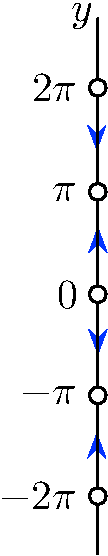
\includegraphics[height=150pt]{images/module14-equil1.pdf}
	\quad 
	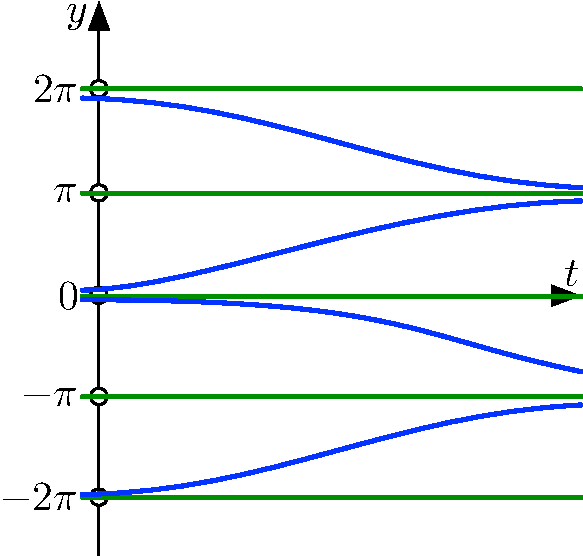
\includegraphics[height=150pt]{images/module14-equil2.pdf}
\end{center}

We can infer that the graphs will approach the constant solutions without touching because the derivative $y'$ will become smaller and smaller the more they approach the equilibria. We also know that solutions cannot touch each other.
\end{example}

There is also a distinction that we make about equilibrium points that helps us understand the behaviour of solutions. We will study this distinction in the core exercises.







\paragraph{\color{cyan}Population Models.} The fact that these differential equations keep the same rate of change independently of time, makes them an ideal candidate when studying populations.

%
%
%
%
%
%
%
%\paragraph{Exponential Growth. } 
%
%
%$P(t) = $ size of a certain population at time $t$
%
%\paragraph{Malthusian Population Model:}
%The population increases/decreases proportionally to its size, i.e.,
%$$
%\frac{dP}{dt} = rP,
%$$
%for some growth rate $r$.
%
%The solution of this DE is
%%    
%%    This is a separable $DE$, so we can solve it:
%%    \begin{align*}
%%    \frac{1}{P} \frac{dP}{dt} & = k \\
%%    \int \frac{1}{P} dP & = \int k dt \\
%%    \ln|P| &= kt + C \\
%%    |P| & = e^{kT+C} = e^C e^{kt} = A e^{kt}
%%    \end{align*}
%%    for $A = e^C >0$.
%%    
%%    So
%\[\tag{Review Exercise}
%P = P(0) e^{rt}.
%\]
%
%\begin{itemize}
%\item Population grows exponentially if $r>0$;
%\item Population decays exponentially if $r<0$.
%\end{itemize}
%
%This method is good while the environment can provide for all the population. Since there are no infinite environments, this method will ultimately fail! 
%
%
%\paragraph{Logistic Model:} Modification of the Malthusian model, to model an environment with limited resources. The individuals in the population are competing for resources among themselves:
%$$
%\frac{dP}{dt} = rP - \alpha P^2,
%$$
%where $P^2$ gives the number of possible encounters between individuals, and $\alpha$ gives a constant on how competition decreases the growth. 
%
%Another way to obtain this model is by observing that the rate of growth decreases as the population increases, so the simplest way to substitute $r$ with $r-\alpha P$ not the Malthusian Model. We obtain
%$$
%\frac{dP}{dt} = (r-\alpha P) P.
%$$
%
%Usually we write $\alpha = \frac rK$, so the model is
%\[\tag{Logistic Growth}
%\frac{dP}{dt} = r P \left(1 - \frac{P}{K}\right),
%\]
%for some intrinsic growth rate $r>0$ (the growth rate without limiting factors).
%
%This equation has two equilibrium solutions:
%$$
%P(t) = 0 \qquad \text{ and } \qquad P(t) = K.
%$$
%
%
%From the equation we observe the following: \\
%
%\begin{minipage}{10cm}
%\begin{itemize}
%\item The solutions cannot cross the line $y=K$: if they did, at $y=K$ they would have $y'=0$ and would remain at $y=K$
%
%\item Look the function $f(P) = \frac rK y(K-y)$ and analyze its sign:
%
%\item if $0<y(0)<K$, then $y' = f(y) > 0$, so the solution will keep increasing
%\item if $y(0)>K$, then $y' = f(y) < 0$, so the solution will keep decreasing
%
%\end{itemize}
%\end{minipage}
%\hfill
%\begin{minipage}{175pt}
%\includegraphics*[width=175pt]{figures/0205_auton.pdf}
%\end{minipage}
%
%\hfill\\
%
%We can now classify the equilibrium solutions:
%\begin{itemize}
%\item $P=0$ is unstable
%\item $P=K$ is stable
%\end{itemize}
%
%
%We can then conclude that the solutions will look like:
%\begin{center}
%\includegraphics*[width=150pt]{figures/0205_logpop.pdf}
%\end{center}
%
%\begin{rem}
%And the constant $K$ is the maximum number of individuals that the environment can sustain.
%\end{rem}
%
%
%We can solve this separable equation to obtain
%%
%%
%%\begin{gather*}
%%\frac{dP}{dt} = \frac rK P \left(K-P\right) \\
%%\frac{1}{P(K-P)} \frac{dP}{dt} = \frac rK \\
%%\\
%%\frac{1}{P(K-P)} = \frac AP + \frac{B}{K-P} \\
%%1 = A(K-P) + BP\\
%%AK=1\\
%%BK=1\\
%%\\
%%\left( \frac{1}{P} + \frac{1}{K-P}\right) \frac{dP}{dt} = r \\
%%\\
%%\ln|P| - \ln|K-P| = r t +C\\
%%\frac{P}{K-P} = c e^{rt} \\
%$$
%P(t) = \frac{K}{1+ce^{-rt}} 
%$$
%%\end{gather*}
%
%
%%
%%
%%To simplify the notation, we relabel the equation to
%%$$
%%\frac{dP}{dt} = P \left(a-bP\right),
%%$$
%%for $a,b>0$.
%%
%%
%%
%%This DE is separable, so we can solve it:
%%\begin{align*}
%%\frac{1}{P(a-bP)} \frac{dP}{dt} & = 1 \\
%%\int \frac{1}{P(a-bP)} dP & = \int 1 dt = t+C.
%%\end{align*}
%%
%%Using partial fractions, we write
%%\begin{align*}
%%\frac{1}{P(a-bP)}
%%	& = \frac{A}{P} + \frac{B}{a-bP} \\
%%	& = \frac{ A(a-bP) + BP}{P (a-bP)} \\
%%	& = \frac{ Aa + (B-Ab)P}{P (a-bP)}.
%%\end{align*}
%%
%%So $Aa = 1$ and $B-Ab = 0$. We have
%%$$
%%A = \frac{1}{a} \qquad \text{ and } \qquad B = \frac{b}{a}.
%%$$
%%
%%We now have
%%$$
%%\int \frac{1}{P(a-bP)} dP
%%	 = \int \frac{1}{a} \left(\frac{1}{P} + \frac{b}{a-bP}\right) dP
%%	 = \frac{1}{a} \left( \ln |P| - \ln |a-bP| \right)
%%	 = \frac{1}{a} \ln \left| \frac{P}{a-bP}\right|
%%$$
%%
%%The solution of the DE is given by
%%\begin{align*}
%%\frac{1}{a} \ln \left| \frac{P}{a-bP}\right| & = t+C \\
%%\ln \left| \frac{P}{a-bP}\right| & = at+aC \\
%%\left| \frac{P}{a-bP}\right| & = e^{aC}e^{at} = C_1 e^{at}
%%\end{align*}
%%for $C_1=e^{aC}>0$.
%%
%%We have
%%$$
%%\frac{P}{a-bP} =  \pm C_1 e^{at} = C_2 e^{at}.
%%$$
%%
%%Now we solve for $P$:
%%\begin{align*} 
%%P & = C_2 e^{at} (a-bP) \\
%%\left( 1 +C_2 b e^{at} \right) P & = C_2 a e^{at} \\
%%P & = \frac{C_2 a e^{at}}{1 +C_2 b e^{at}} \\
%%P & = \frac{a}{b + \frac{1}{C_2} e^{-at}}
%%\end{align*}
%%
%%We know that $\ds C_2 = \frac{P(0)}{a-bP(0)}$, so
%%$$
%%P(t) = \frac{a}{b + \left(\frac{a}{P(0)}-b\right) e^{-at}} 
%%= \frac{K}{1 + \left(\frac{K}{P(0)}-1\right) e^{-rt}}.
%%$$
%%
%%We can verify that $P(t) \to K$ as $t \to \infty$.
%\begin{note}
%We can improve on these models. For example, we can include a threshold of survivability, where if a population goes below that level, it will eventually become extinct.
%
%\subparagraph{Exercise. } Study the model
%$$
%\frac{dP}{dt} = -r\left(1-\frac PT\right) \left(1-\frac PK\right) P,
%$$
%where $r>0$ and $0<T<K$.
%\end{note}
%
%
%
%\paragraph{``Jelly Fish'' from MAT187. } 
%
%
%On a question of a midterm on MAT187, we studied another DE for a ``jelly fish'' population:
%$$
%\frac{dP}{dt} = r(P-T)(P-K)^2,
%$$
%for $0<T<K$.
%
%We can quickly study this problem qualitatively by studying the function: $f(y) =  r(y-T)(y-K)^2$.
%
%The equilibrium points are:
%$$
%T \quad , \quad K\quad .
%$$
%We study the sign of $f(y)$:
%
%\begin{center}
%\includegraphics*[width=200pt]{figures/0202_jellyfish.pdf}
%\hfil
%\includegraphics*[width=150pt]{figures/0202_jellyfish_sols.pdf}
%\end{center}
%
%We can also classify the equilibrium solutions:
%\begin{itemize}
%\item $P=T$ is unstable
%\item $P=K$ is semi-stable (stable from below and unstable from above)
%\end{itemize}
%
%
%And we can analyze the solutions:
%\begin{itemize}
%\item If $0< P_0 < T$, then the population will go extinct (in finite time). It doesn't just approach extinction asymptotically, it really does go extinct, as the slope keeps increasing (with negative sign)
%
%\item If $T<P<K$, then the population thrives and increases its number approaching $P=K$.
%
%\item If $T>K$, then the population increases at an accelerating pace. It goes ``viral''!
%\end{itemize}
%
%
%
%\subparagraph{Exercise. } Read Pages 81--83: Critical points and stable/unstable equilibrium solutions.



\begin{video}
\begin{itemize}
	\item \qrvideo{https://youtu.be/swt-let4pCI} %\href{https://youtu.be/swt-let4pCI}{https://youtu.be/swt-let4pCI} \hfill \qrcode{https://youtu.be/swt-let4pCI}
\end{itemize}	
\end{video}




	\begin{exercises}

	\begin{problist}
	\prob Show that all autonomous differential equations are separable.
	
	\prob Consider the ODE $y'=\displaystyle \frac1y$.
	Then which of the statements below are true or false and justify your choice.
	\begin{enumerate}
		\item The solutions always stay positive.
		\item The solutions always stay negative.
		\item The solutions never change sign.
		\item The solutions always change sign.
		\item Some solutions change sign, and some don't.
	\end{enumerate}
	
	\prob Sketch a slope field for the autonomous ODE $$y'=\cos(y).$$
	\prob Sketch a slope field for the autonomous ODE $$y'=\tan(y).$$
	\prob What is a common property of all slope fields of autonomous ODEs?
	
	
	\prob Consider the ODE
	$$ 
	y' = {\rm sign}(y) = 
		\begin{cases}
			1 & \text{ if } y > 0 \\	
			0 & \text{ if } y = 0 \\	
			-1 & \text{ if } y < 0
		\end{cases}. 
	$$

	\begin{enumerate}
		\item What are the equilibrium solutions?
		\item Find two solutions that satisfy $y(0)=0$.
		\item Are there solutions that satisfy $\displaystyle \lim_{t \to \infty} y(t) = \pi$?
		\item What are the possible limits of solutions as $t\to \infty$?
	\end{enumerate}
	
%		y=0 sol
%		y=max(0,t+c) sol
%		y=min(0,-t+c) sol




	\prob \label{mod14-q-stable}Consider a function $f(y)$ such that
	\begin{itemize}
		\item $f(1)=0$;
		\item $f'$ is continuous for all $y$;
		\item $f'(1)<0$.
	\end{itemize}
	\begin{enumerate}
		\item Show that there is an open interval $(a,b)$ satisfying $1 \in (a,b)$ and $f'(y)<0$ for all $y \in (a,b)$.
		\item Show that %there is an interval $(c,d) \subseteq (a,b)$ such that
		\begin{itemize}
%			\item $1 \in (c,d)$, 
			\item $f(y)>0$ if $y \in (a,1)$, %(c,1)$,
			\item $f(y)<0$ if $y \in (1,b)$. %(1,d)$.
		\end{itemize}
		\item Consider the initial-value problem $y'=f(y)$ with $y(0)=y_0$. Show that this problem has a unique solution.
		\item Show that if $y_0 \in (a,b)$, then $\displaystyle \lim_{t \to \infty} y(t) = 1$.
		\item Write a Theorem about equilibrium points based on the results of this question.
	\end{enumerate}


	\prob Consider a function $f(y)$ such that
	\begin{itemize}
		\item $f(2)=0$;
		\item $f'$ is continuous for all $y$;
		\item $f'(2)>0$.
	\end{itemize}
	
	Complete a study similar to question \ref{mod14-q-stable} for this function $f$.
	
	
	
	\prob Consider an autonomous ODE $y'=f(y)$ with two stable equilibrium solutions $y=1$ and $y=2$ and where $f$ is continuous.
	\begin{enumerate}
		\item Show that there must exist another equilibrium point $c \in (1,2)$.
		\item Show that if $f(y)\not\equiv 0$ in $(1,2)$, then there must exist an equilibrium point $c \in (1,2)$ that is either semi-stable or unstable.
	\end{enumerate}

	\end{problist}
\end{exercises}



%	\Heading{Motivation} 



\end{module}



\begin{lesson}
	\Title{Autonomous Differential Equations}

%	\Heading{Objectives}
%	\begin{itemize}
%		\item The second step in Mathematical modelling is to construct a representation of how the team will be attempting to solve the problem.
%		\item Create a mind map of the problem. This is a structured way to brainstorm possible solutions and their requirements.
%	\end{itemize}
%	
%	\Heading{Motivation} 
%
%\begin{annotation}
%	\begin{goals}
%	\Goal{Extra Reading}
%	Math Modelling: Getting started and getting solutions, Bliss-Fowler-Galluzzo
%	
%	\hfill \qrcode{https://m3challenge.siam.org/resources/modeling-handbook}	
%	\end{goals}
%\end{annotation}
%	\Heading{Extra Reading} \href{https://m3challenge.siam.org/resources/modeling-handbook}{Math Modelling: Getting started and getting solutions, Bliss-Fowler-Galluzzo}

\end{lesson}




\newpage

\question Consider the differential equation \quad $y'=f(y)$ \quad where $f(y)$ is given by the following graph:
\begin{center}
	\includegraphics*[width=350pt]{images/module14-graphf.pdf}
\end{center}

\begin{parts}
	\item What are the equilibrium points?
	\item Which equilibrium solutions are stable, unstable, or semi-stable?
	\item Write a definition for a \textbf{stable}, \textbf{unstable}, and \textbf{semi-stable} equilibrium point.
	\item Roughly, sketch a solution satisfying:
	\begin{enumerate}
		\item $y(0)=2.5$.
		\item $y(0)=-\frac14$.
		\item $y(1)=\frac14$.
	\end{enumerate}
	\item If $y(0) = 2$, then $y(t) = $
	\item If $y(0) = \frac12$, then $\displaystyle \lim_{t\to \infty} y(t) = $
	\item If $y(0) = -2$, then $\displaystyle \max_{t \in [0,\infty)} y(t) = $
\end{parts}


\bookonlynewpage


\hfill


\bookonlynewpage



%
%
%%%%%%%%%%%%%%%%%%%%%%%%%%%%%%%%%%%%%%%%%%%%%%%%%%%%%%%%%%%%%%%%%%%%%%%%%
%%		Analyzing ODEs
%
%
%\begin{module}{Analysis of Differential Equations}
%	%\Title{First-Order Linear ODEs}
%%	\Heading{Textbook}	
%%	\Heading{Objectives}
%%	\begin{itemize}
%%		\item Bla bla bla	
%%	\end{itemize}
%
%	\label{odes-analysis}
%
%	In this module you will learn
\begin{itemize}
	\item different ways to analyze differential equations
\end{itemize}

\hfill \\



In this chapter, we have learned how to create models involving ODEs, how to solve some special types of ODEs


%	\input{modules/module15-AnalysisODEs-exercises.tex}
%
%
%
%%	\Heading{Motivation} 
%
%
%
%\end{module}
%
%
%
%\begin{lesson}
%	\Title{Analysis of Differential Equations}
%
%%	\Heading{Objectives}
%%	\begin{itemize}
%%		\item The second step in Mathematical modelling is to construct a representation of how the team will be attempting to solve the problem.
%%		\item Create a mind map of the problem. This is a structured way to brainstorm possible solutions and their requirements.
%%	\end{itemize}
%%	
%%	\Heading{Motivation} 
%%
%%\begin{annotation}
%%	\begin{goals}
%%	\Goal{Extra Reading}
%%	Math Modelling: Getting started and getting solutions, Bliss-Fowler-Galluzzo
%%	
%%	\hfill \qrcode{https://m3challenge.siam.org/resources/modeling-handbook}	
%%	\end{goals}
%%\end{annotation}
%%	\Heading{Extra Reading} \href{https://m3challenge.siam.org/resources/modeling-handbook}{Math Modelling: Getting started and getting solutions, Bliss-Fowler-Galluzzo}
%
%\end{lesson}
%
%
%
%
%\newpage
%
%\question 
%	Bla!
%
%







%%%%%%%%%%%%%%%%%%%%%%%%%%%%%%%%%%%%%%%%%%%%%%%%%%%%%%%%%%%%%%%%%%%%%%%%
%
%		Chapter 3 - First-order Systems
%
%%%%%%%%%%%%%%%%%%%%%%%%%%%%%%%%%%%%%%%%%%%%%%%%%%%%%%%%%%%%%%%%%%%%%%%%




%%%%%%%%%%%%%%%%%%%%%%%%%%%%%%%%%%%%%%%%%%%%%%%%%%%%%%%%%%%%%%%%%%%%%%%%
%
%		Chapter 3 - System Models
%
%%%%%%%%%%%%%%%%%%%%%%%%%%%%%%%%%%%%%%%%%%%%%%%%%%%%%%%%%%%%%%%%%%%%%%%%


\begin{topic}[Models of Systems]



\vfil

\begin{center}
\begin{minipage}{300pt}
	\includegraphics*[width=300pt]{images/chap3-xkcd.png}

	\hfill {\footnotesize (image from \href{https://www.xkcd.com/2063/}{xkcd - comic \#2063})}
\end{minipage}
\end{center}


\end{topic}






%%%%%%%%%%%%%%%%%%%%%%%%%%%%%%
%
%  MODULE - Modelling Two Interconnected Quantities
%
%%%%%%%%%%%%%%%%%%%%%%%%%%%%%%



\begin{module}{Modelling Two Quantities}
	\label{sys:model}

	In this module you will learn
\begin{itemize}
	\item how to model two or more inter-dependent quantities using systems
\end{itemize}

\hfill \\


Often, when modelling something, we are faced with two or more quantities that depend on each other. This means that one equation is not enough, so we need to learn how to deal with a system of equations. \\


Just like we did in module \ref{model-odes}, we will follow the step by step procedure developed in chapter 1.

\paragraph{\emph{Step 1.}} Define the problem

\begin{example}
We want to model two interacting populations, like the populations of bears and salmon in a specific natural park.\\

The first step is to decide on what we want to find at the end of the process. 
In this case, we want to know the number of individuals in each population and how they change as time passes. So we define:
\begin{itemize}
	\item $b(t) =$ number of bears in the natural park at time $t$;
	\item $s(t) =$ number of salmon in the natural park at time $t$.
\end{itemize}
\end{example}


\paragraph{\emph{Step 2.}} Build a mind map

\begin{example}
We start with both species in the centre:

\def\SalmonBear{
	\fill[color=orange!50!white] (-4,0) rectangle (-2,1) node[pos=.5] {\color{black}Salmon};
	\fill[color=brown!60!white] (4,0) rectangle (2,1) node[pos=.5] {\color{black}Bear};
}
\begin{center}
\begin{tikzpicture}
	\SalmonBear
\end{tikzpicture}
\end{center}

We can start brainstorming about the things that affect these populations:
\begin{center}
%\begin{tikzpicture}
%	\SalmonBear
%    \begin{scope}[decoration={
%    markings,
%    mark=at position 0.5 with {\arrow{>}}}
%    ]
%	\draw[postaction={decorate}] (-2,1) arc (120:60:4) node[pos=0.5,above] {food};
%    \draw[postaction={decorate}] (2,0) arc (300:240:4) node[pos=0.5,below] {hunts};
%    \end{scope}
%    \draw (-3,0) -- (-4,-1);
%    \fill[color=green!50!white] (-5.25,-2) rectangle (-2.75,-1) node[pos=.5] {\color{black}reproduction};
%    \draw (-3,1) -- (-4,2);
%    \fill[color=yellow!50!white] (-5.25,2) rectangle (-2.75,3) node[pos=.5] {\color{black}habitat limits};
%    \draw (3,0) -- (4,-1);
%    \fill[color=red!50!white] (5.25,-2) rectangle (2.75,-1) node[pos=.5] {\color{black}competition};
%    \draw (3,1) -- (4,2);
%    \fill[color=yellow!50!white] (5.25,2) rectangle (2.75,3) node[pos=.5] {\color{black}habitat limits};
%\end{tikzpicture}
\begin{tikzpicture}
	\SalmonBear
    \begin{scope}[decoration={
    markings,
    mark=at position 0.5 with {\arrow{>}}}
    ]
    \draw[postaction={decorate}] (-2,0.5) -- (2,0.5) node[pos=0.5,above] {food};
    \draw[postaction={decorate}] (2,0) arc (300:240:4) node[pos=0.5,below] {hunts};
    \end{scope}
    \draw (-3,0) -- (-4,-1);
    \fill[color=green!50!white] (-5.25,-2) rectangle (-2.75,-1) node[pos=.5] {\color{black}reproduction};
    \draw (-3,1) -- (-0.5,2);
    \draw (3,1) -- (0.5,2);
    \fill[color=yellow!50!white] (-1.5,2) rectangle (1.5,3) node[pos=.5] {\color{black}habitat limits};
    \draw (3,0) -- (4,-1);
    \fill[color=red!50!white] (5.25,-2) rectangle (2.75,-1) node[pos=.5] {\color{black}competition};
\end{tikzpicture}
\end{center}
	
\end{example}


\paragraph{\emph{Step 3.}} Make assumptions

\begin{example}
In this step, we discuss which of the boxes in the mind map we want to actually consider in our model, and which assumptions we need to make to consider them. \\

Let us start with how these species interact with each other:
\begin{enumerate}
	\item Salmon provide food for bears: the bear population profits from each encounter with salmon. How does each bear-salmon encounter affect the bear population?
	\item Bears hunt salmon: the salmon population is likely to decrease with each encounter with a bear. How does each bear-salmon encounter affect the salmon population?
\end{enumerate}

These two components are essential in our model, so we need to include them. It still leaves some freedom on how to do this. \\

There are other elements that we might want to include in our model:
\begin{enumerate}[start=3]
	\item Salmon reproduction: in the absence of predators and under ideal conditions, salmon should grow according to the Malthusian model, i.e. the rate of growth is proportional to the number of salmon;
	\item Bear competition: bears are mainly predators, so without salmon, their numbers will decrease, also according to the Malthusian model;
	\item Habitat limits: these species live in habitats that have limited resources, so we can consider a carrying capacity for each species.
\end{enumerate}

To make the model simpler, we will \emph{ignore habitat limits}. This means that this model will not be accurate if the populations become very large.
	
\end{example}


\paragraph{\emph{Step 4.}} Construct a model

\begin{example}
We will start with our populations:
\begin{itemize}
	\item $b(t)$
	\item $s(t)$
\end{itemize}
and we will start adding components to each of these one by one. \\

For the first two items, we need to estimate the number of encounters salmon-bear. We assume that the number of encounters is proportional to the number of all possible encounters: \emph{$b(t)\, s(t)$}.

\begin{enumerate}
	\item Salmon provide food for bears: for every possible salmon-bear encounter, there is a probability that a bear actually encounters a salmon, and then there is a chance that the bear will catch the salmon. Each catch improves the possibility that the bear population will increase. All these put together means that this factor should increase the bear growth rate by \emph{$a \,b(t)\, s(t)$}, where the constant $a$ needs to be found.
	\item Bears hunt salmon: similarly to the previous item, for every possible encounter, there is a probability that the bear actually encounters a salmon, and then there is a chance that the bear will catch the salmon. Every catch will decrease the salmon population, so the salmon growth rate will decrease by \emph{$c \,b(t) \,s(t)$}, there the constant $c$ needs to be found.
\end{enumerate}

Right now we have the following model:
$$
\begin{cases}
b'(t) = a \,b(t)\, s(t) + \cdots \\
s'(t) = - c \,b(t)\, s(t) + \cdots	
\end{cases}
$$

We continue with the other elements:
\begin{enumerate}[start=3]
	\item Salmon reproduction: this was explained before and should contribute to the salmon growth rate with the term \emph{$d s(t)$}.
	\item Bear competition: this was also explained above and should contribute to the bear growth rate with the term \emph{$-e b(t)$}.
	\item Habitat limits: we decided to ignore this.
\end{enumerate}

We have the model:
$$
\begin{cases}
b'(t) = a \, b(t) \,s(t) -e \, b(t) \\
s'(t) = - c \, b(t) \,s(t) + d \, s(t)
\end{cases}
$$

To find the constants $a,c,d,e$, we would probably need to go back to Step 3 and make further assumptions related to the way that we are measuring them.
\end{example}



\paragraph{\emph{Step 5.}} Model assessment

\begin{example}

We can do several things here. 

One of the things that we can do is approximate its solutions using Euler's Method discussed in Module \ref{Approximation}. 

Let us assume, for this example the constants: $a=1$, $e=10$, $c=1$, $d=5$ and a time step $\Delta t = 0.5$ and we assumed an initial population of $b(0)=6$ and $s(0)=9$. Then we obtain the graph below:


\begin{center}
\includegraphics*[width=200pt]{images/module16-lotka-volterra.png}
\end{center}
\begin{itemize}
	\item \url{https://www.desmos.com/calculator/zywspwstwk} \hfill \qrcode{https://www.desmos.com/calculator/zywspwstwk}
\end{itemize}

The $x-$axis is the bear population while the $y-$axis is the salmon population. Each dot gives an approximation of the populations $\Delta t = 0.5$ time units after the previous approximation.\\


From this approximation, we can say infer that this model creates a population cycle, but it seems to spiral outwards: 
\begin{center}
\includegraphics*[width=200pt]{images/module16-lotka-volterra-more.png}
\end{center}

\begin{itemize}
	\item Is having a population cycle a feature that our model should have?
	\item Is the spiralling outwards a feature we want in our model?
	\item Is the spiralling a feature of the model or the approximation? If it's from the approximation, how does the model behave?
\end{itemize}

I'll let you brainstorm and think of other ways you can assess this model.
\end{example}

\begin{graybox}
There are lots of other tools to create slope fields and approximate solutions of systems of ODEs.

\begin{itemize}
	\item GeoGebra approximation of the same model, called the Lotka-Volterra model:
	
	\hfill \qrvideo{https://www.geogebra.org/m/KqNV7eHB}
	
	\item WolframAlpha slope field of the same model:

	\hfill \qrvideo{https://uoft.me/modelling-sys-wa}

	\item WolframAlpha stream plot of the same model:

	\hfill \qrvideo{https://uoft.me/modelling-sys-wa2}
	
	\item There are also better methods of approximating ODEs and systems, e.g. \href{https://en.wikipedia.org/wiki/Runge-Kutta_methods}{Runge-Kutta methods} 
	
	\hfill \qrvideo{https://en.wikipedia.org/wiki/Runge-Kutta_methods}
\end{itemize}

\end{graybox}


%\paragraph{\emph{Step 6.}} Putting it all together in a report
%
%We'll skip this part here.
%




	\begin{exercises}

	\begin{problist}
	
	\prob Create a model for two cooperating populations, like sharks and remoras. 
	
	
%	\begin{center}
%		\includegraphics*[height=150pt]{images/module15-spring-mass-dashpot.pdf}
%	\end{center}
	
	
	\begin{minipage}{.35\textwidth}
		\prob We have a spring attached to a mass and with a dashpot. 
		\begin{enumerate}
			\item Model the position of the mass as time changes.
			\item Obtain a system of two first-order ODEs. Remember to explain how the new functions relate to the spring-mass-dashpot system.
		\end{enumerate}
	\end{minipage}
	\hfill
	\begin{minipage}{100pt}
		\includegraphics*[height=100pt]{images/module16-spring-mass-dashpot.pdf}
	\end{minipage}

	\prob Model a vehicle with a special engine that provides an acceleration to the car proportional to the fuel left.
	
	\prob Imagine two twin babies and model their crying volume. Assume that they naturally become tired and stop crying if alone, but they cry more if the other twin is crying.
	
	
	
	\begin{minipage}{.35\textwidth}
		\prob Create a simplified model for a tree, considering the height of the tree and its leaf area and how they affect each other.	
	\end{minipage}
	\hfill
	\begin{minipage}{100pt}
		\includegraphics*[height=100pt]{images/module16-tree.pdf}
	\end{minipage}

	\prob Create a model on how a student's confidence in her own ability affects her learning/knowledge of a subject. Remember the Ebbinghaus' ``forgetting curve''.

	\begin{center}
		\includegraphics*[width=125pt]{images/module16-UofT2YYZ.pdf}	
	\end{center}

	\prob Imagine that there are two ways to travel from UofT to Toronto's Pearson airport (YYZ). Both paths take the same time if there is no traffic. You want to direct people on the fastest path. Create a model for choosing the fastest path.
	
	
	\prob Create a model for the sales of a specific brand of sneakers. The goal is to capture the influence of famous people and non-famous people on each other's purchases.
	
	\prob Create a model on how the population and the cost of living in Toronto affect each other.
	
	
	\end{problist}
\end{exercises}

\end{module}



\begin{lesson}
	\Title{Modelling Two Quantities}

	\Heading{Objectives}
	\begin{itemize}
		\item Bla
	\end{itemize}
	
	\Heading{Motivation} 

\end{lesson}




\newpage

\question We want to model two competing populations, like cheetahs and lions: they don't hunt each other, but they hunt the same prey.
\begin{parts}
	\item Create a model for these two populations.
	\item Using Desmos or WolframAlpha, create a slope field in the plane where the horizontal axis is one population and the vertical one is the other.
	\item Using the slope field, deduce some properties of your model and discuss how closely it matches what you expect from these populations.

	\item Extend the model to include a population of antelopes.	
\end{parts}





\bookonlynewpage


\question
	A cheetah is chasing an antelope. We want a model of their positions as they run.
	
	
\begin{annotation}
	\begin{goals}
		This exercise is not required to do in lecture.
		
		Allow some brainstorming and try to create a structure for this problem:
		\begin{itemize}
			\item Positions seen from above ($xy-$plane).
			\item Only need $x_a(t), y_a(t)$ and $x_c(t), y_c(t)$
			\item Focus on the cheetah: where is she heading to?
			\item For the antelope, students need to come up with an escape strategy
			\item Model will be nonlinear!
		\end{itemize}
	\end{goals}
\end{annotation}





%%%%%%%%%%%%%%%%%%%%%%%%%%%%%%
%
%  MODULE - Solving Systems
%
%%%%%%%%%%%%%%%%%%%%%%%%%%%%%%



\begin{module}{Systems of two linear ODEs with constant coefficients}
	\label{sys:solve}

	In this module you will learn
\begin{itemize}
	\item how to solve systems of two linear first-order ODEs with constant coefficients
\end{itemize}

\hfill \\


First, a system of two first-order ODEs has the form:
$$
\begin{cases}
x'(t) = f\big(t, x(t),y(t)\big) \\	
y'(t) = g\big(t, x(t),y(t)\big)
\end{cases}
$$
where the functions $f$ and $g$ are continuous and have continuous derivatives. \\

This system could be nonlinear, so we are only considering linear systems with constant coefficients, which means that they have a very specific form:
$$
\begin{cases}
	x'(t) = a x(t) + b y(t) + e\\
	y'(t) = c x(t) + d y(t) + f
\end{cases}
%
\quad \Leftrightarrow \quad 
	\begin{bmatrix} x'(t) \\ y'(t) \end{bmatrix}
	=
	\begin{bmatrix} a & b \\ c & d \end{bmatrix}
	\begin{bmatrix} x(t) \\ y(t) \end{bmatrix}
	+	\begin{bmatrix} e \\ f \end{bmatrix}
%
\quad \Leftrightarrow \quad 
	\vec{r}'(t)
	=
	A \, \vec{r}(t) + \vec{b}
$$
where
$$
\vec{r}(t) = \begin{bmatrix} x(t) \\ y(t) \end{bmatrix}
\quad , \quad 
A = \begin{bmatrix} a & b \\ c & d \end{bmatrix}
\quad and \quad 
\vec{b}=\begin{bmatrix} e \\ f \end{bmatrix}.
$$

The unknown functions we are trying to find is $\vec{r}(t)$. \\


\paragraph{\emph{Homogeneous Systems.}} These are systems of the form above with $\vec{b} = \vec{0}$.

This means that we want to find all functions $\vec{r}(t)$ that satisfy
$$
\vec{r}'(t) = A \vec{r}(t).
$$


\begin{example}
Let us start with an example of the same problem where $\vec{r}(t)$ is a ``one-dimensional'' vector, a scalar function $u(t)$, and the matrix $A$ is a ``one-dimensional matrix'', a constant $a$. \\

We want to solve the problem	
$$
u'(t) = a \cdot u(t).
$$

We have seen how to solve these kind of problems before. The solutions are
$$
u(t) = c e^{at},
$$
where $c$ can be any constant.
\end{example}

In our two-dimensional case, it is a little more complicated. We can't just write $e^{At}$ where $A$ is a matrix (this expression can make sense, but we would have to find out what is the exponential of a matrix). \\

So we can use the example above to make an \emph{educated guess}: the solution should look like an exponential:
$$
\vec{r}(t) = 
\vec{c} \, e^{\lambda t},
$$
where $\vec{c}$ is a constant vector. \\

If our guess is correct, to find $\vec{r}(t)$, we only need to find $\lambda$ and $\vec{c}$. \\

Let us see what happens when we use this guess and plug it into the system of ODEs:
\begin{align*}
\vec{r}'(t) = A \vec{r}(t) \quad
	& \Leftrightarrow \quad \vec{c} \lambda e^{\lambda t} = A \vec{c} e^{\lambda t} \\
	& \Leftrightarrow \quad \vec{c} \lambda = A \vec{c}.
\end{align*}

This is a problem you have seen before -- and eigenvalue-eigenvector problem: 
\begin{itemize}
	\item $\lambda$ can be any eigenvalue of the matrix $A$
	\item $\vec{c}$ can be any eigenvector of $A$ associated with $\lambda$ 
\end{itemize}

This means that we might have multiple choices for eigenvalues and eigenvectors, or even that eigenvalues and eigenvectors involve complex numbers.
Let us split our study of possible solutions in three cases.



%%%%%%%%%       %%%%%%%%%       %%%%%%%%%       %%%%%%%%%       %%%%%%%%%

\subsection{Two real and distinct eigenvalues}

\begin{example}
Consider the problem
$$
\vec{r}'(t) = \begin{bmatrix}	
 10 & 18 \\ -6 & -11	
 \end{bmatrix} \, \vec{r}(t).
$$

Then, the eigenvalues and eigenvectors of the matrix are
\begin{itemize}
	\item $\lambda_1=-2$ with eigenvector $\vec{v}_1 = \begin{bmatrix} 3 \\ -2 \end{bmatrix}$
	\item $\lambda_2=1$ with eigenvector $\vec{v}_2 = \begin{bmatrix} 2 \\ -1 \end{bmatrix}$
\end{itemize}

This means that we found two solutions:
$$
\vec{r}_1(t) = \begin{bmatrix} 3 \\ -2 \end{bmatrix} e^{-2t}
\quad \text{ and } \quad \vec{r_2}(t) = \begin{bmatrix} 2 \\ -1 \end{bmatrix} e^{t}.
$$

Then, we can show that 
$$
\vec{r}(t) = c_1 \begin{bmatrix} 3 \\ -2 \end{bmatrix} e^{-2t}
+c_2\begin{bmatrix} 2 \\ -1 \end{bmatrix} e^{t}
$$
is also a solution of the problem for any constants $c_1$ and $c_2$.

In fact, we can show that this formula captures all possible solutions for this problem.
\end{example}


\begin{video}
	\begin{itemize}
		\item \qrvideo{https://youtu.be/YUjdyKhWt6E}
	\end{itemize}
\end{video}




%%%%%%%%%       %%%%%%%%%       %%%%%%%%%       %%%%%%%%%       %%%%%%%%%

\subsection{Two complex eigenvalues}

We actually don't need to know a lot about complex numbers to be able to understand how to solve this case.
The results about complex values that are necessary to know will be included in the box below.

\begin{definition}[Complex numbers]
\begin{itemize}
	\item A complex number is a number of the form $z=a+ib$ where $i$ is called the imaginary constant and satisfies $i^2=-1$.
	\item Given a complex number $z=a+ib$, we call $\overline{z}=a-ib$ its complex conjugate. It satisfies:
	$$ z \cdot \overline{z} = a^2+b^2 = |z|^2.$$

	\item If a matrix has real components and two complex eigenvalues, then the eigenvalues are complex conjugates of each other. Moreover, the eigenvectors are also complex conjugates of each other.
	\item Euler's Formula: $e^{i \theta} = \cos(\theta) + i \sin (\theta)$.
\end{itemize}
\end{definition}




\begin{example}
Consider the problem
$$
\vec{r}'(t) = \begin{bmatrix}	
 1 & 1 \\ -1 & 1
 \end{bmatrix} \, \vec{r}(t).
$$

Then, the eigenvalues and eigenvectors of the matrix are
\begin{itemize}
	\item $\lambda_1=1+i$ with eigenvector $\vec{v}_1 = \begin{bmatrix} -i \\ 1 \end{bmatrix}$
	\item $\lambda_2=1-i$ with eigenvector $\vec{v}_2 = \begin{bmatrix} i \\ 1 \end{bmatrix}$
\end{itemize}

This means that we found two solutions:
$$
\vec{r}_1(t) = \begin{bmatrix} -i \\ 1 \end{bmatrix} e^{(1+i)t}
\quad \text{ and } \quad \vec{r}_2(t) = \begin{bmatrix} i \\ 1 \end{bmatrix} e^{(1-i)t}.
$$

Then, all solutions of this system of ODEs can be expressed as
$$
\vec{r}(t) = c_1 \begin{bmatrix} -i \\ 1 \end{bmatrix} e^{(1+i)t}
+c_2\begin{bmatrix} i \\ 1 \end{bmatrix} e^{(1-i)t}.
$$

There is a problem with the form of these solutions: they involve complex numbers!

Imagine that we start with a problem where we have two (real) quantities that interact with each other through this system of differential equations.
Then we expect these quantities to measure in real numbers, not complex.

\begin{itemize}
	\item This means that we expect \emph{the imaginary part of this solutions to cancel out}.
\end{itemize}

So let us manipulate this formula using Euler's formula and see if we can re-write in such a way that doesn't involve complex numbers. \\

We have:
\begin{align*}
	e^{(1+i)t} &= e^t \cdot e^{it} = e^t \big( \cos(t) + i \sin(t)\big) \\
	e^{(1-i)t} &= e^t \cdot e^{-it} = e^t \big( \cos(t) - i \sin(t)\big)
\end{align*}

So our solution expands to:
$$
\vec{r}(t) = c_1 \begin{bmatrix} -i \\ 1 \end{bmatrix} e^t \big( \cos(t) + i \sin(t)\big)
+c_2\begin{bmatrix} i \\ 1 \end{bmatrix} e^t \big( \cos(t) - i \sin(t)\big).
$$

We can now manipulate this expression:
\begin{align*}
\vec{r}(t) 
	& = e^t
		\begin{bmatrix}
			-i c_1 	\big( \cos(t) + i \sin(t)\big) + i c_2 \big( \cos(t) - i \sin(t)\big) \\
			c_1 	\big( \cos(t) + i \sin(t)\big) + c_2 \big( \cos(t) - i \sin(t)\big) \\
		\end{bmatrix} \\
	& = e^t 
		\begin{bmatrix}
			(c_1+c_2) \sin(t) - i (c_1-c_2) \cos(t) \\
			(c_1+c_2) \cos(t) + i(c_1-c_2) \sin(t)
		\end{bmatrix} \\
	& = e^t \left( (c_1+c_2) \begin{bmatrix} \sin(t) \\ \cos(t) \end{bmatrix}
		+ i (c_1 -c_2) \begin{bmatrix} - \cos(t) \\ \sin(t) \end{bmatrix}
		\right)
\end{align*}

So now we do something that might look like a ``cheating''. We define:
$$
a_1 = c_1+c_2 \quad \text{ and } \quad a_2 = i (c_1-c_2).
$$


Then the solution is
$$
\vec{r}(t) = a_1\begin{bmatrix} \sin(t) \\ \cos(t) \end{bmatrix} e^t
		+ a_2 \begin{bmatrix} - \cos(t) \\ \sin(t) \end{bmatrix} e^t.
$$

This last form doesn't include any complex numbers and is equivalent to the previous form.

\end{example}

\begin{graybox}
	It may look like the final solution above still includes complex numbers in the constants $a_1$ and $a_2$. 
	
	To convince yourself that this is not the case, solve the following exercise.\\
	
	Find the unique solution of
	$$
	\vec{r}'(t) = \begin{bmatrix}	
 		1 & 1 \\ -1 & 1
		\end{bmatrix} 
		\, \vec{r}(t)
	\qquad \text{ with} \qquad
	\vec{r}(0) = \begin{bmatrix}
 			-3 \\ 2
	 \end{bmatrix}
	 $$
	 
	 Find the constants $c_1, c_2$ and then the constants $a_1,a_2$. Which ones are complex and which ones are real?
\end{graybox}

\begin{video}
	\begin{itemize}
		\item \qrvideo{https://youtu.be/TRVS5Wo9LoM}
	\end{itemize}
\end{video}



%%%%%%%%%       %%%%%%%%%       %%%%%%%%%       %%%%%%%%%       %%%%%%%%%

\subsection{One real repeated eigenvalue}


\begin{example}
Consider the problem
$$
\vec{r}'(t) = \begin{bmatrix}	
 5 & 0 \\ 1 & 5	
 \end{bmatrix} \, \vec{r}(t).
$$

Then, there is only one eigenvalue with one eigenvector
\begin{itemize}
	\item $\lambda_1=5$ with eigenvector $\vec{v}_1 = \begin{bmatrix} 0 \\ 1 \end{bmatrix}$, which yield a solution $\vec{r}_1(t) = c_1 \begin{bmatrix} 0 \\ 1 \end{bmatrix} e^{5t}$.
\end{itemize}

This is a \emph{problem} because we need two solutions to put together and obtain two constants, as in the two previous cases.
%\end{example}

\begin{graybox}
To convince yourself that it is a problem, try solving the problem above with initial conditions
$$
\vec{r}(0) = \begin{bmatrix}	0 \\ 4 \end{bmatrix}.
$$

What about with initial conditions
$$
\vec{r}(0) = \begin{bmatrix}	 1 \\ 4 \end{bmatrix} \quad ?
$$
\end{graybox}

%\begin{example}

This means that we ware missing one solution -- that will enable us to solve the problem for any initial conditions. \\


Let us re-write the original problem in a different form by letting 
$$
\vec{r}(t) = \begin{bmatrix} x(t) \\ y(t)\end{bmatrix}.
$$
Then we have
$$
\begin{cases}
x'(t) = 5 x(t) \\
y'(t) = x(t) +5 y(t)	
\end{cases}
$$
These are two ODEs, but we can solve the first and then tackle the second one.
We obtain
$$
\begin{cases}
	x(t) = c_2 e^{5t} \\
	y(t) = 	c_1 e^{5t} + c_2 t e^{5t} 
\end{cases}
\quad \Leftrightarrow \quad
	\vec{r}(t) = \begin{bmatrix}
		c_2 \\ c_1 + c_2 t
	\end{bmatrix} e^{5t}
\quad \Leftrightarrow \quad
	\vec{r}(t) = c_1 \begin{bmatrix} 0 \\ 1 \end{bmatrix} e^{5t} + c_2
	\begin{bmatrix}	1 \\ t
	\end{bmatrix} e^{5t}
$$
\end{example}

\begin{graybox}
Observe that the solution we found has the form:
$$
	\vec{r}(t) = \underbrace{c_1 \begin{bmatrix} 0 \\ 1 \end{bmatrix} e^{5t}}_{\text{solution } \vec{r}_1(t)} + c_2 \left( 
	\underbrace{\begin{bmatrix}	1 \\ 0 \end{bmatrix}}_{\text{new vector } \vec{w}} e^{5t} + \underbrace{\begin{bmatrix} 0  \\ 1 
	\end{bmatrix}}_{\vec{v}_1} t e^{5t}\right).
$$

So we can make another \emph{educated guess} that the solution we were missing has the form:
$$
\vec{r}_2(t) = \left(\vec{w} + \vec{v}_1 t\right) e^{\lambda t}.
$$

With this form in mind, we can plug it into the system of ODEs \quad $\vec{r}'(t) = A \vec{r}(t)$ \quad, which has exactly one eigenvalue $\lambda$, to get:
$$
\lambda \vec{w}e^{\lambda t} + \lambda \vec{v}_1 t e^{\lambda t} + \vec{v}_1 e^{\lambda t}
= A \vec{w} e^{\lambda t} + A \vec{v}_1 t  e^{\lambda t}
$$
which is equivalent to:
$$
\lambda \vec{w} + \underbrace{\lambda \vec{v}_1}_{=A \vec{v}_1} t  + \vec{v}_1
= A \vec{w}  + A \vec{v}_1 t 
	\quad \Leftrightarrow \quad
	\left( \lambda I - A \right ) \vec{w} = \vec{v}_1
$$
%which becomes
%$$
%\lambda \vec{w} + \vec{v}_1
%= A \vec{w}  
%	\quad \Leftrightarrow \quad
%	\left( \lambda I - A \right ) \vec{w} = \vec{v}_1
%$$

Since at this point we already know $\lambda$ and $\vec{v}_1$, we can now find $\vec{w}$ in a similar way used to find the eigenvector $\vec{v}_1$. The vector $\vec{w}$ is called a \emph{generalized eigenvector} of $A$ associated with the eigenvalue $\lambda$.

\end{graybox}

\begin{video}
	\begin{itemize}
		\item \qrvideo{https://youtu.be/hCShTLmeZN4}
	\end{itemize}
\end{video}






	\begin{exercises}

	\begin{problist}
	\prob \label{mod17-gensol}Find the general solution of the problem $\vec{r}'(t) = A \vec{r}(t)$ for the following matrices:
	\begin{enumerate}
	\begin{minipage}{.2\textwidth}
		\item $A = \begin{bmatrix} -7 & 6 \\ -9 & 8 \end{bmatrix}$;
		\item $A = \begin{bmatrix} 22 & 24 \\ -15 & -16\end{bmatrix}$;
		\item $A = \begin{bmatrix} 0 & 1 \\ -5 & 0 \end{bmatrix}$;
		\item $A = \begin{bmatrix} 0 & 1 \\ 5 & 0 \end{bmatrix}$;
		\item $A = \begin{bmatrix} 1 & \sqrt{3} \\ \sqrt{3} & -1\end{bmatrix}$;
		\item $A = \begin{bmatrix} 1 & \sqrt{3} \\ -\sqrt{3} & 1\end{bmatrix}$;
	\end{minipage}
	\qquad
	\begin{minipage}{.2\textwidth}
		\item $A = \begin{bmatrix} 0 & 1 \\ -4 & -4 \end{bmatrix}$;
		\item $A = \begin{bmatrix} -4 & -6 \\ 2 & 3 \end{bmatrix}$;
		\item $A = \begin{bmatrix} 2 & -3 \\ 0 & 2 \end{bmatrix}$;
		\item $A = \begin{bmatrix} 2 & 0 \\ 0 & 2 \end{bmatrix}$;
		\item $A = \begin{bmatrix} 0 & 0 \\ 1 & 0\end{bmatrix}$; 
		\item $A = \begin{bmatrix} 0 & 0 \\ 0 & 1\end{bmatrix}$; 
	\end{minipage}
	\end{enumerate}

	\prob For each of the problems in the previous exercise, find the solution that satisfies the initial conditions:
	\begin{enumerate}[label=(\roman*)]
		\item $\vec{r}(0)=\begin{bmatrix} 0 \\ 0 \end{bmatrix}$;
		\item $\vec{r}(0)=\begin{bmatrix} 1 \\ 3 \end{bmatrix}$;
		\item $\vec{r}(1)=\begin{bmatrix} -2 \\ 2 \end{bmatrix}$.
	\end{enumerate}


	\prob Consider the problem $\vec{r}'(t) = \begin{bmatrix} 2 & 0 \\ 1 & 3 \end{bmatrix} \vec{r}(t) + \begin{bmatrix} -2 \\ 11 \end{bmatrix}$.
	\begin{enumerate}
		\item Show that $\vec{e}(t) = \begin{bmatrix} 1 \\ -4 	\end{bmatrix}$ is a solution of this problem.
		\item Find the general solution of 
		$$\vec{u}'(t) = \begin{bmatrix} 2 & 0 \\ 1 & 3 \end{bmatrix} \vec{u}(t).$$
		\item Let $\vec{r}(t) = \vec{u}(t) + \vec{e}(t)$. Show that this is a solution of the original problem.
		\item Let $\vec{r}_1(t)$ and $\vec{r}_2(t)$ be two solutions of the original problem. 
		\begin{enumerate}
			\item Is $\vec{r}_1(t) + \vec{r_2}(t)$ a solution? 
			\item Is $3\vec{r}_1(t) $ a solution? 
			\item Write a result on how one can safely combine solutions of non-homogeneous problems.
		\end{enumerate}
	\end{enumerate}

	
	\prob \label{prob:sys-nonhomogeneous}Consider the problem  \quad $\vec{r}'(t) = \begin{bmatrix} 1 & 2 \\ 3 & 0 \end{bmatrix}
 \vec{r}(t)+\begin{bmatrix} -5 \\ 3 \end{bmatrix}
$.
	\begin{enumerate}
		\item Observe that this system is an autonomous system of ODEs. What is the equilibrium solution? 
		\item Let the equilibrium solution solution you just found be called $\vec{e}$. Consider $\vec{u}(t) = \vec{r}(t) - \vec{e}$, where $\vec{r}(t)$ is the solution of the original problem. Show that 
			$$ \vec{u}'(t) = A \, \vec{u}(t).$$
		\item Find $\vec{u}(t)$.
		\item Find $\vec{r}(t)$.
		\item Write a procedure to solve any problem of the form
			$$ \vec{r}(t) = A \, \vec{r}(t) + \vec{b}. $$
	\end{enumerate}
	
	
	\prob \label{prob:sys-superposition}Consider the problem \quad $\vec{r}'(t) = A \, \vec{r}(t)$.
	Assume that we have two solutions $\vec{r_1}(t)$ and $\vec{r_2}(t)$.
	\begin{enumerate}
		\item Show that $\vec{r}(t) = \vec{r_1}(t) + \vec{r_2}(t)$ is a solution also.
		\item Show that $\vec{r}(t) = 2\vec{r_1}(t) - 3\vec{r_2}(t)$ is a solution also.
		\item Find all possible solutions of the problem.
	\end{enumerate}
	
	
		\prob Consider the problem $\vec{r}'(t) = \begin{bmatrix} 1 & -2 \\ -2 & 1 \end{bmatrix} \vec{r}(t)$.
		\begin{enumerate}
			\item Find the solution that satisfies the initial condition $\vec{r}(0)=\begin{bmatrix}1 \\ 0\end{bmatrix}$. Call it $\vec{u}(t)$.
			\item Find the solution that satisfies the initial condition $\vec{r}(0)=\begin{bmatrix}0 \\ 1\end{bmatrix}$. Call it $\vec{v}(t)$.
			\item Define the matrix function
			$$ \Phi(t) = \begin{bmatrix} \vec{u}(t) \; | \; \vec{v}(t) \end{bmatrix} = \begin{bmatrix} u_1(t) & v_1(t) \\ u_2(t) & v_2(t) \end{bmatrix}.$$
			
			Show that $\vec{r}(t) = \Phi(t) \vec{r}_0$ is a solution of the original system of ODEs. Which initial condition does it satisfy?
			
			\item Write a result relating $\Phi(t)$ to the solution of initial-value problems.
			\end{enumerate}

	
	
		\prob \label{mod17:prob-W1}Consider a system of ODEs $\vec{r}'(t) = A \vec{r}(t)$ with two solutions $\vec{r}_1(t)$ and $\vec{r}_2(t)$. 
		
		We want to study the conditions that are necessary on the solutions $\vec{r}_1$ and $\vec{r}_2$ to guarantee that we can solve any initial-value problem.
		
		\begin{enumerate}
			\item What is the general solution for this problem?
			\item If the initial condition is $\vec{r}(0)= \begin{bmatrix} 1 \\ 2 \end{bmatrix}$, then what are the conditions on $\vec{r}_1,\vec{r}_2$ ?
			\item If the initial condition is $\vec{r}(0)= \vec{r_0}$, then what are the conditions on $\vec{r}_1,\vec{r}_2$ ?
		\end{enumerate}

		\prob Consider a system of ODEs $\vec{r}'(t) = A \vec{r}(t)$ with two solutions $\vec{r}_1(t), \vec{r}_2(t)$.
		
			Let $R(t)$ be the matrix 
				$R(t) = \begin{bmatrix} \vec{r}_1(t) & | & \vec{r}_2(t)	\end{bmatrix} $ 
				and let $W(t) = \det R(t)$.
		
		\begin{enumerate}
			\item Show that $W(t)$ is a solution of $W' = (a_{11} + a_{22}) W$.
			\item Solve the ODE above to obtain an expression for $W(t)$.
			\item Show that $W(t)$ is either identically zero, or it's never zero. 
			\item Use this result to simplify your answer to problem \ref{mod17:prob-W1}(c).
		\end{enumerate}
	
	\end{problist}
\end{exercises}

\end{module}



\begin{lesson}
	\Title{Systems of two linear ODEs with constant coefficients}

	\Heading{Objectives}
	\begin{itemize}
		\item Bla
	\end{itemize}
	
	\Heading{Motivation} 

\end{lesson}




\newpage

\question
Consider a cheetah-lion inspired problem:
$$
\frac{d \,\vec{r}}{dt} = \begin{bmatrix} 3 & -2 \\ -1 & 4\end{bmatrix} \vec{r}.
$$
	
\begin{parts}
	\item Find the two solutions $\vec{r}_1, \vec{r}_2$.
	\item Is $\vec{r}_1(t) + \vec{r}_2(t)$ a solution?
	\item Is $\vec{r}_1(t) - \vec{r}_2(t)$ a solution?
	\item Is $2\vec{r}_1(t) + 3\vec{r}_2(t)$ a solution?
	\item What is the general solution?
	\item Find the solution that satisfies $\vec{r}(0) = \begin{bmatrix} 6 \\ 7\end{bmatrix}$?
\end{parts}


\bookonlynewpage


\question
Consider a problem:
$$
\frac{d \,\vec{r}}{dt} = \begin{bmatrix} 2 & -5 \\ 1 & -2\end{bmatrix} \vec{r}.
$$
	
\begin{parts}
	\item Find the general solution.
	\item Find the solution that satisfies $\vec{r}(0) = \begin{bmatrix} 6 \\ 7\end{bmatrix}$?
\end{parts}




\bookonlynewpage


\question
Consider a problem:
$$
\frac{d \,\vec{r}}{dt} = \begin{bmatrix} 4 & -1 \\ 8 & -2\end{bmatrix} \vec{r} - \begin{bmatrix} 5 \\ 10 \end{bmatrix}.
$$
%[2,3]
\begin{parts}
	\item Find the equilibrium solution.
	\item Find the general solution.
	\item Find the solution that satisfies $\vec{r}(0) = \begin{bmatrix} 2 \\ 3\end{bmatrix}$?
\end{parts}








%%%%%%%%%%%%%%%%%%%%%%%%%%%%%%
%
%  MODULE - Phase Portraits
%
%%%%%%%%%%%%%%%%%%%%%%%%%%%%%%



\begin{module}{Phase Portraits}
	\label{sys:phase}

	In this module you will learn
\begin{itemize}
	\item how to sketch a phase portrait for a linear system of ODEs with constant coefficients
	\item how to use a phase portrait to deduce properties of solutions
\end{itemize}

\hfill \\

When we solve a system of two ODEs, we obtain two functions $x(t)$ and $y(t)$, so when we want to graph solutions, we have a problem:
\begin{itemize}
	\item Should we sketch each of these functions separately?
	\item Should we sketch them together?
	\item Should we sketch the path as if a particle is moving with coordinates $x(t)$ and $y(t)$?
\end{itemize}

\begin{example}
Consider the initial-value problem
$$
\frac{d\,\vec{r}}{dt} = \begin{bmatrix} 0 & 1 \\ -1 & 0 \end{bmatrix}\vec{r} \quad \text{ with } \quad \vec{r}(0)=\begin{bmatrix} 0 \\ 1 \end{bmatrix},
$$
which has the solution
$$
\vec{r}(t) = \begin{bmatrix}
	\sin(t) \\ \cos(t)
\end{bmatrix}.
$$

Which of the following ways are better?
\begin{itemize}
\item \begin{minipage}{400pt}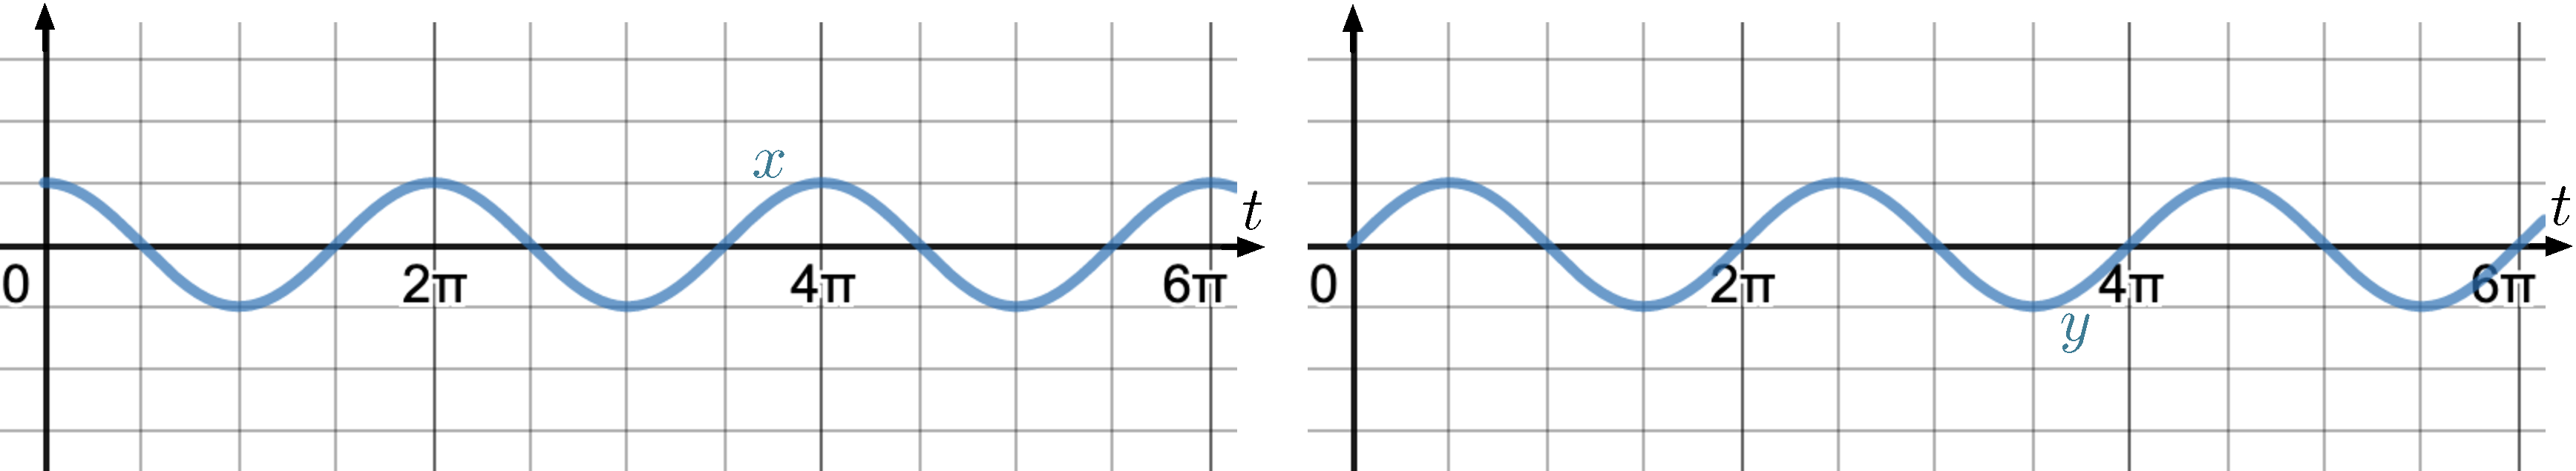
\includegraphics[width=400pt]{images/module18-sep-xy.pdf}\end{minipage}

\item \begin{minipage}{200pt}\includegraphics*[width=200pt]{images/module18-together-xy.pdf}\end{minipage}

\item \begin{minipage}{200pt}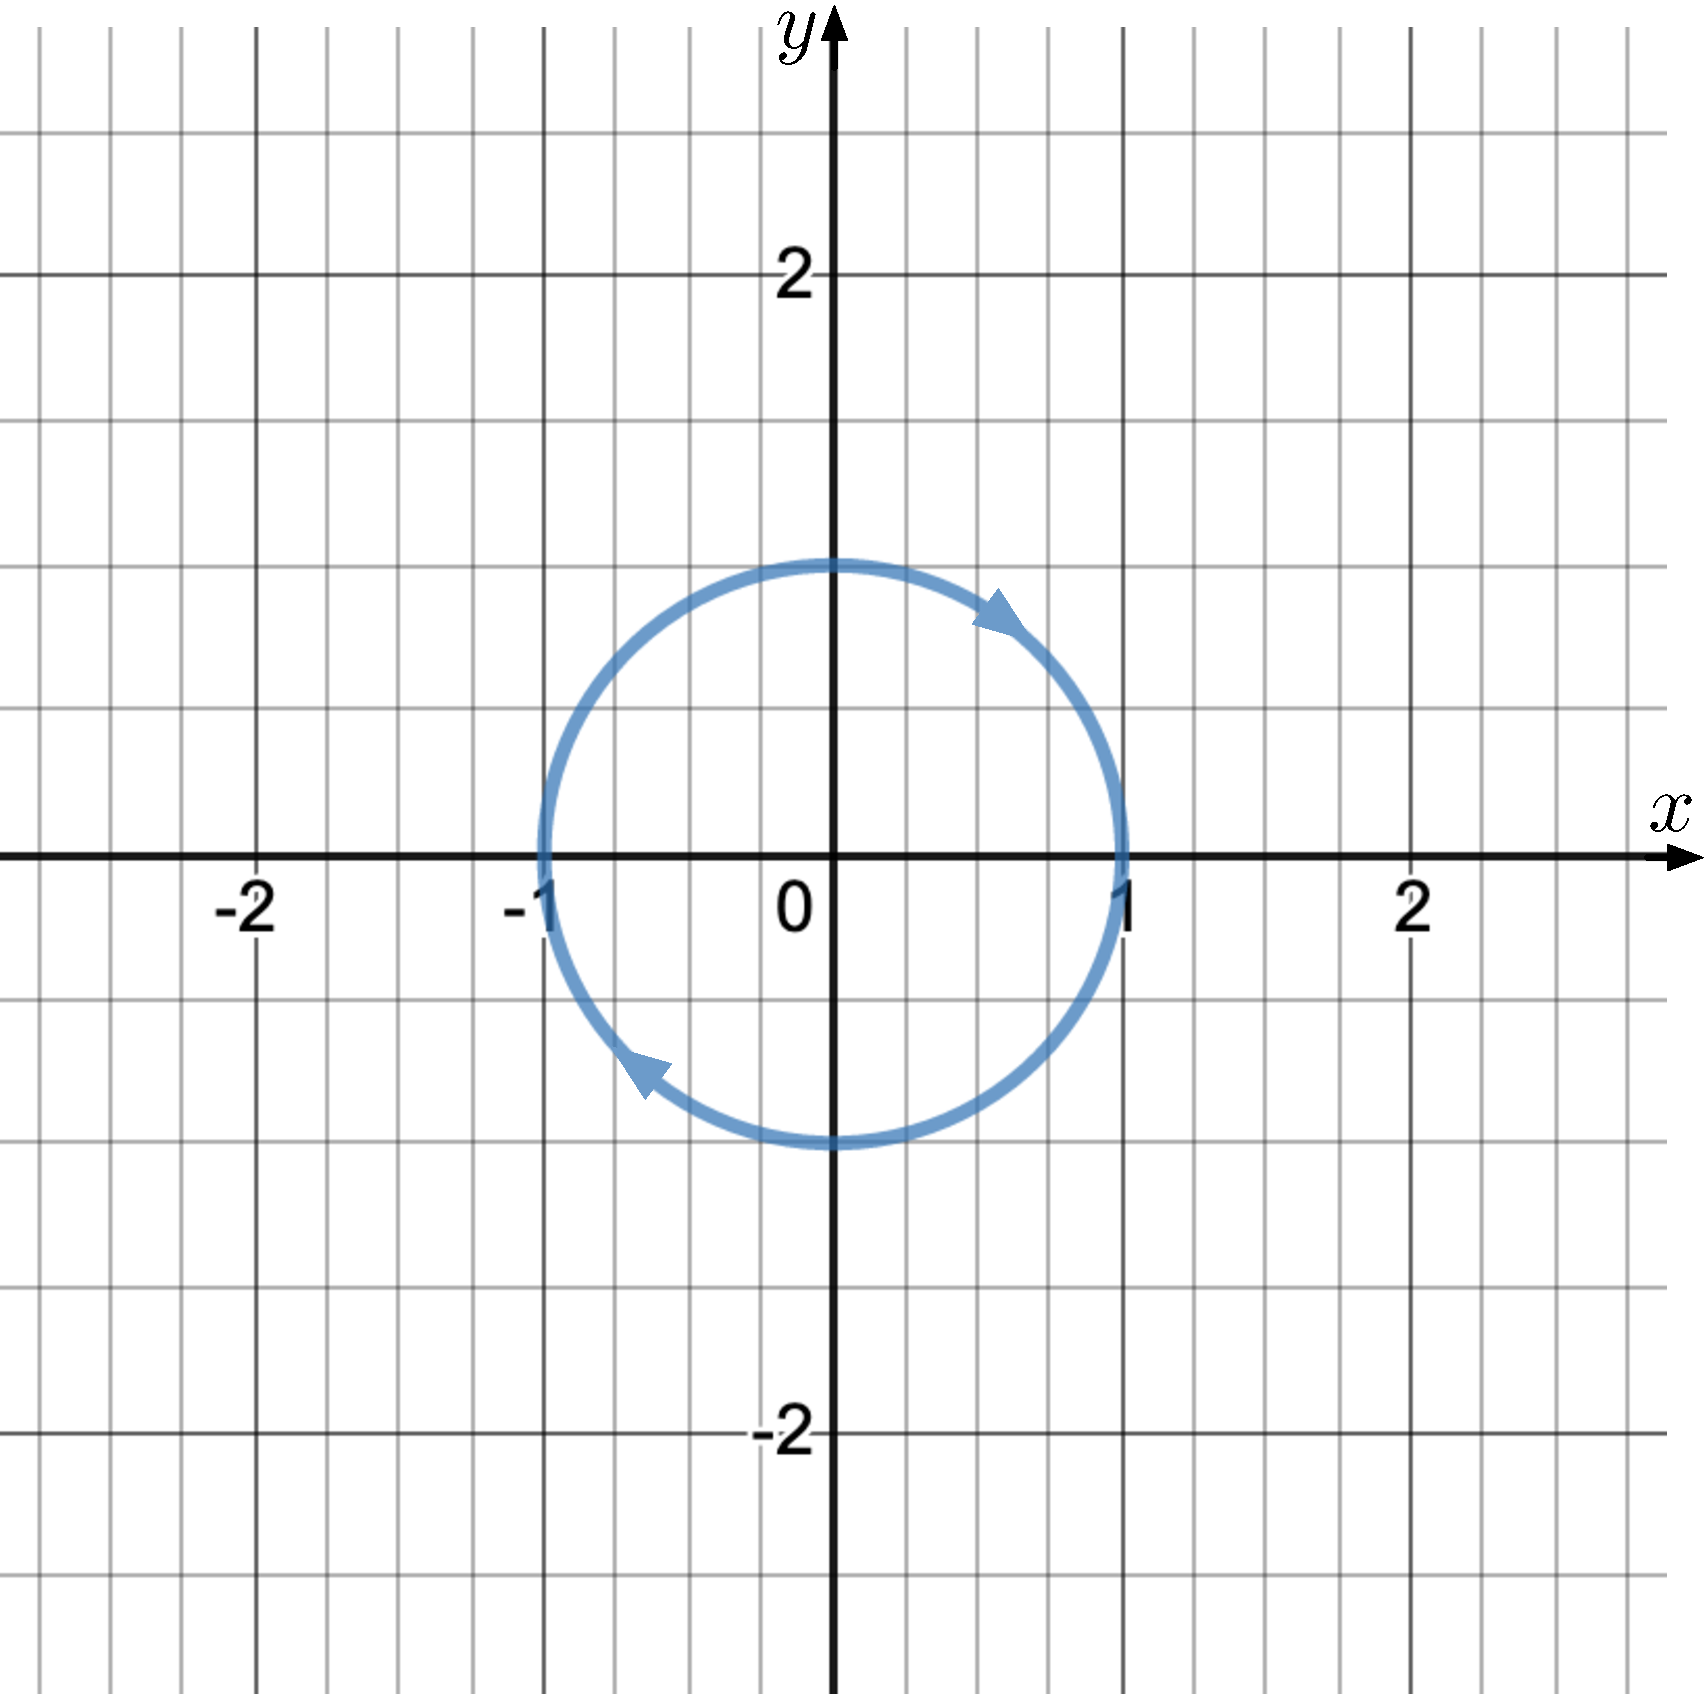
\includegraphics[height=200pt]{images/module18-phaseportrait.pdf}\end{minipage}
\end{itemize}

There is no correct answer, but the last graph gives more information on how the two quantities interact with each other, so we will focus on that type of graph.
\end{example}


The graphs in the example above are graphs of one specific solution. A phase portrait gives an idea of all possible solutions. 
\begin{example}
The last graph of the example is part of which phase portrait?

\begin{center}
\includegraphics*[width=420pt]{images/module18-possiblephaseportraits.pdf}
\end{center}

A phase portrait gives a good idea of how all solutions behave.
\end{example}

Sketching phase portraits for systems of two first-order linear ODEs is important because it gives us insight on how the two components affect each other for all solutions.

\begin{example}
Consider the problem
$$
\frac{d \, \vec{r}}{dt} = \begin{bmatrix} -2 & 3 \\ -3 & -2 \end{bmatrix} \vec{r},
$$
where the matrix $A$ has the eigenvalues and eigenvectors:
\begin{itemize}
	\item Eigenvalues $\lambda_{\pm} = -2 \pm 3i$ with eigenvectors $v_{\pm} = \begin{bmatrix} \mp i \\ 1 \end{bmatrix}$
\end{itemize}

This means that the general solution has the form
\begin{itemize}
	\item $\displaystyle \vec{r}(t) = a_1 \begin{bmatrix} -i \\ 1 \end{bmatrix} e^{(-2+3i)t} + a_2 \begin{bmatrix} i \\ 1 \end{bmatrix} e^{(-2-3i)t}$

	\item[or]
	\item $\displaystyle \vec{r}(t) = c_1 \begin{bmatrix}	 \sin(3t) \\ \cos(3t) \end{bmatrix} e^{-2t} + c_2 \begin{bmatrix}	 -\cos(3t) \\ \sin(3t) \end{bmatrix} e^{-2t}$ \\
\end{itemize}

We can use the general form and start sketching some solutions.

\begin{itemize}
	\item Let $c_1=1$ and $c_2=0$ and we obtain
	$$ \vec{r}(t) = \begin{bmatrix}	 \sin(3t) \\ \cos(3t) \end{bmatrix} e^{-2t}.$$
	
	To sketch this solution, let us start by ignoring the term $e^{-2t}$. 
	
	So we want to sketch $ \vec{r}(t) = \begin{bmatrix}	 \sin(3t) \\ \cos(3t) \end{bmatrix}$:
	\begin{center}
		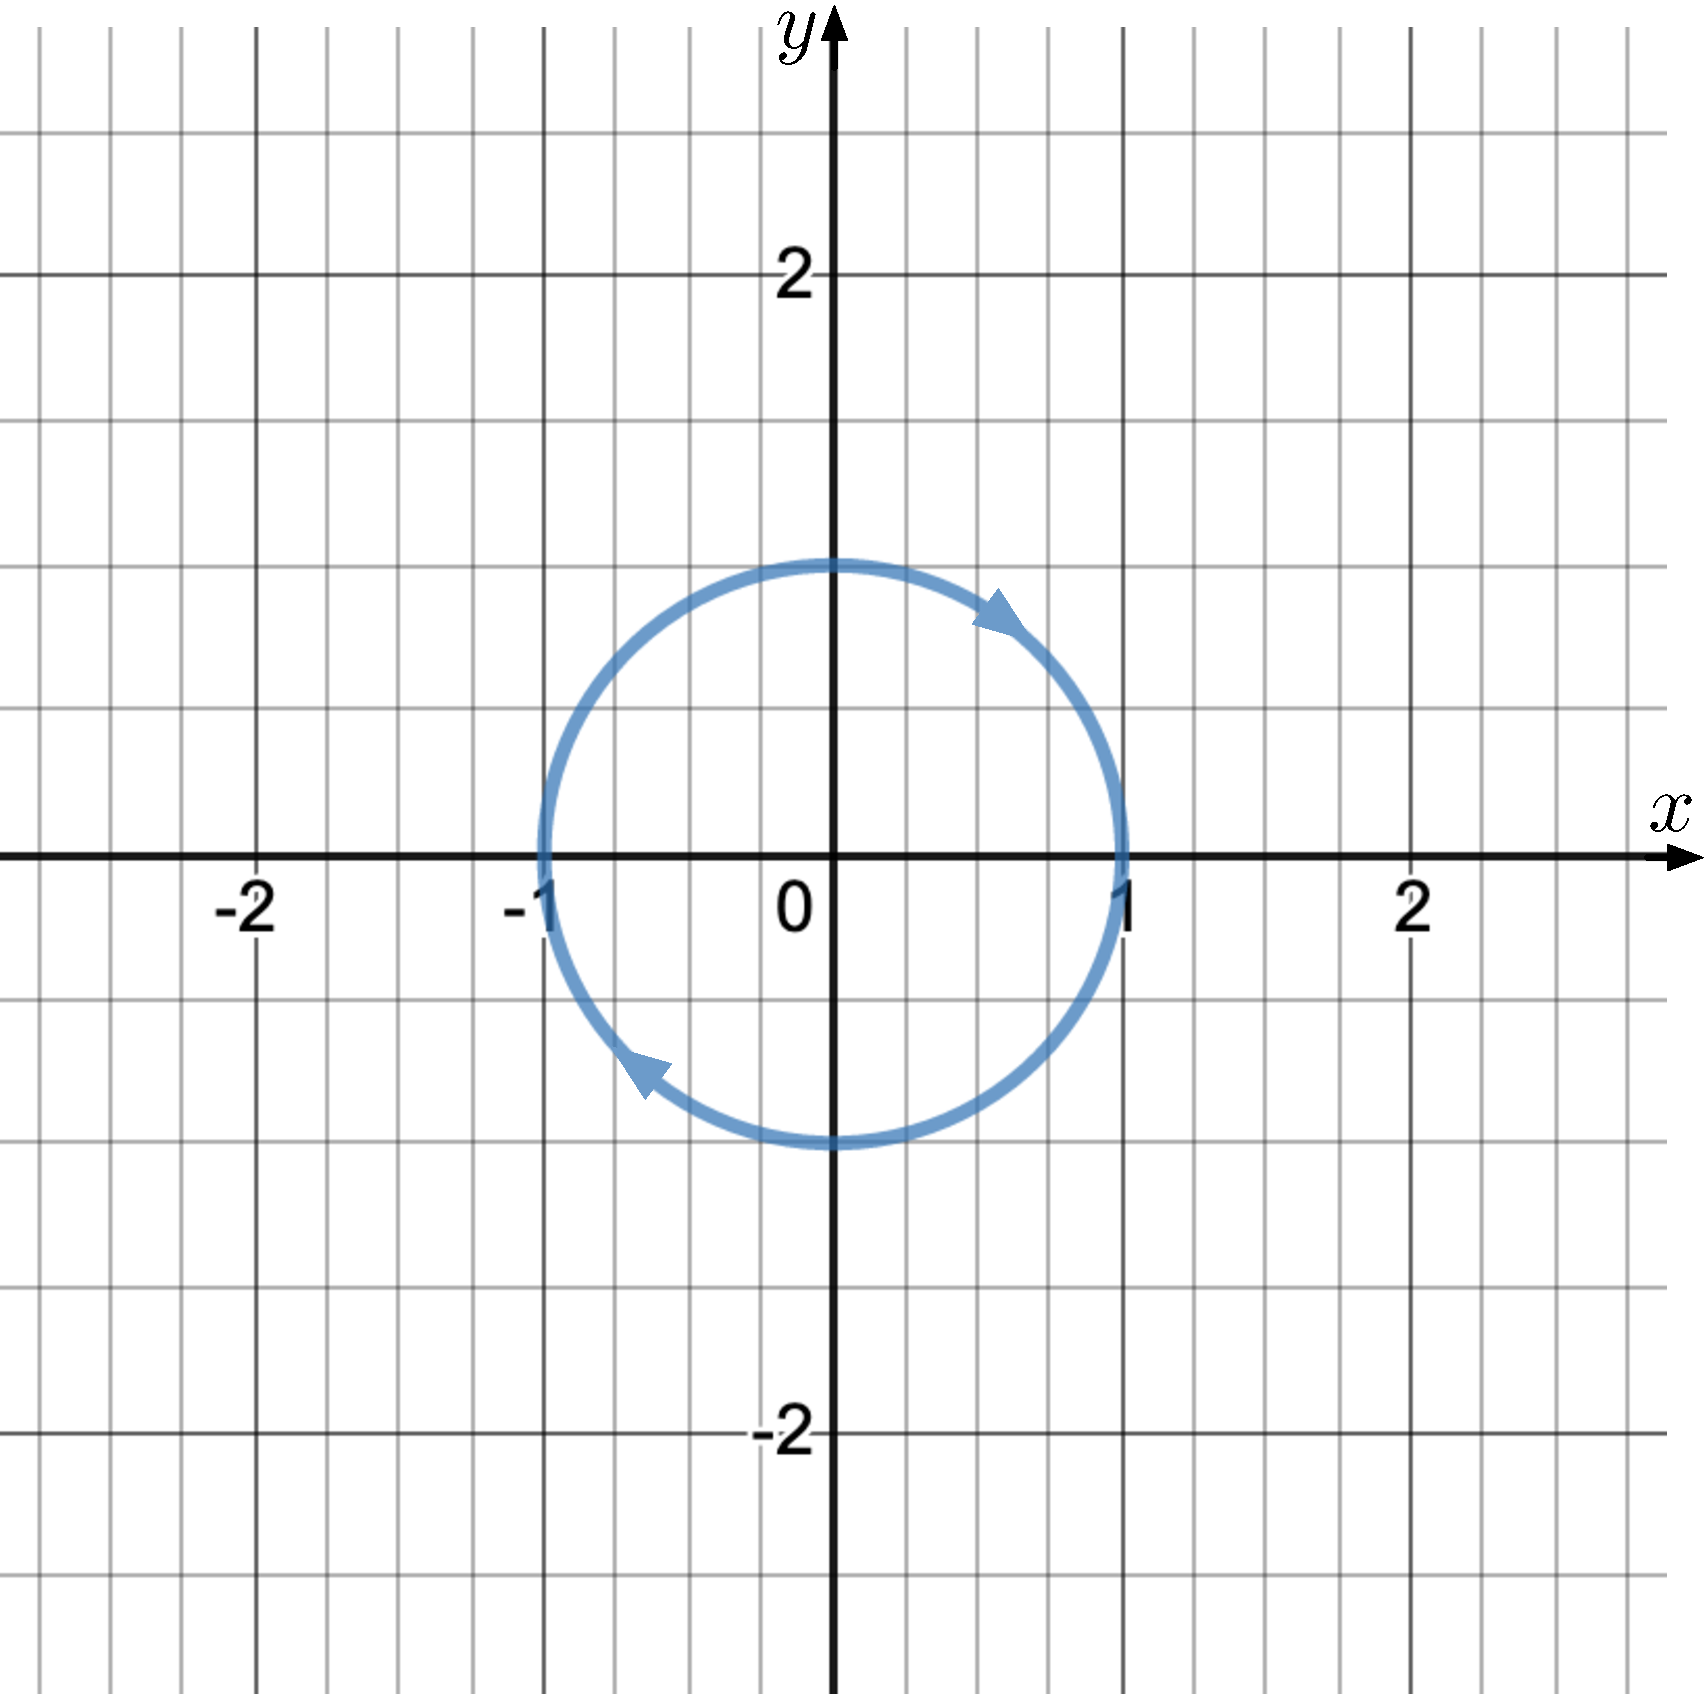
\includegraphics[height=200pt]{images/module18-phaseportrait.pdf}
	\end{center}
	
	The path is going in circles in the clockwise direction.
	
	By multiplying the solution by $e^{-2t}$, which starts at $1$ when $t=0$ and keeps decreasing towards $0$ as $t$ increases, we are creating a graph that keeps revolving around the origin as it converges towards the origin, yielding a spiral.
	\begin{center}
		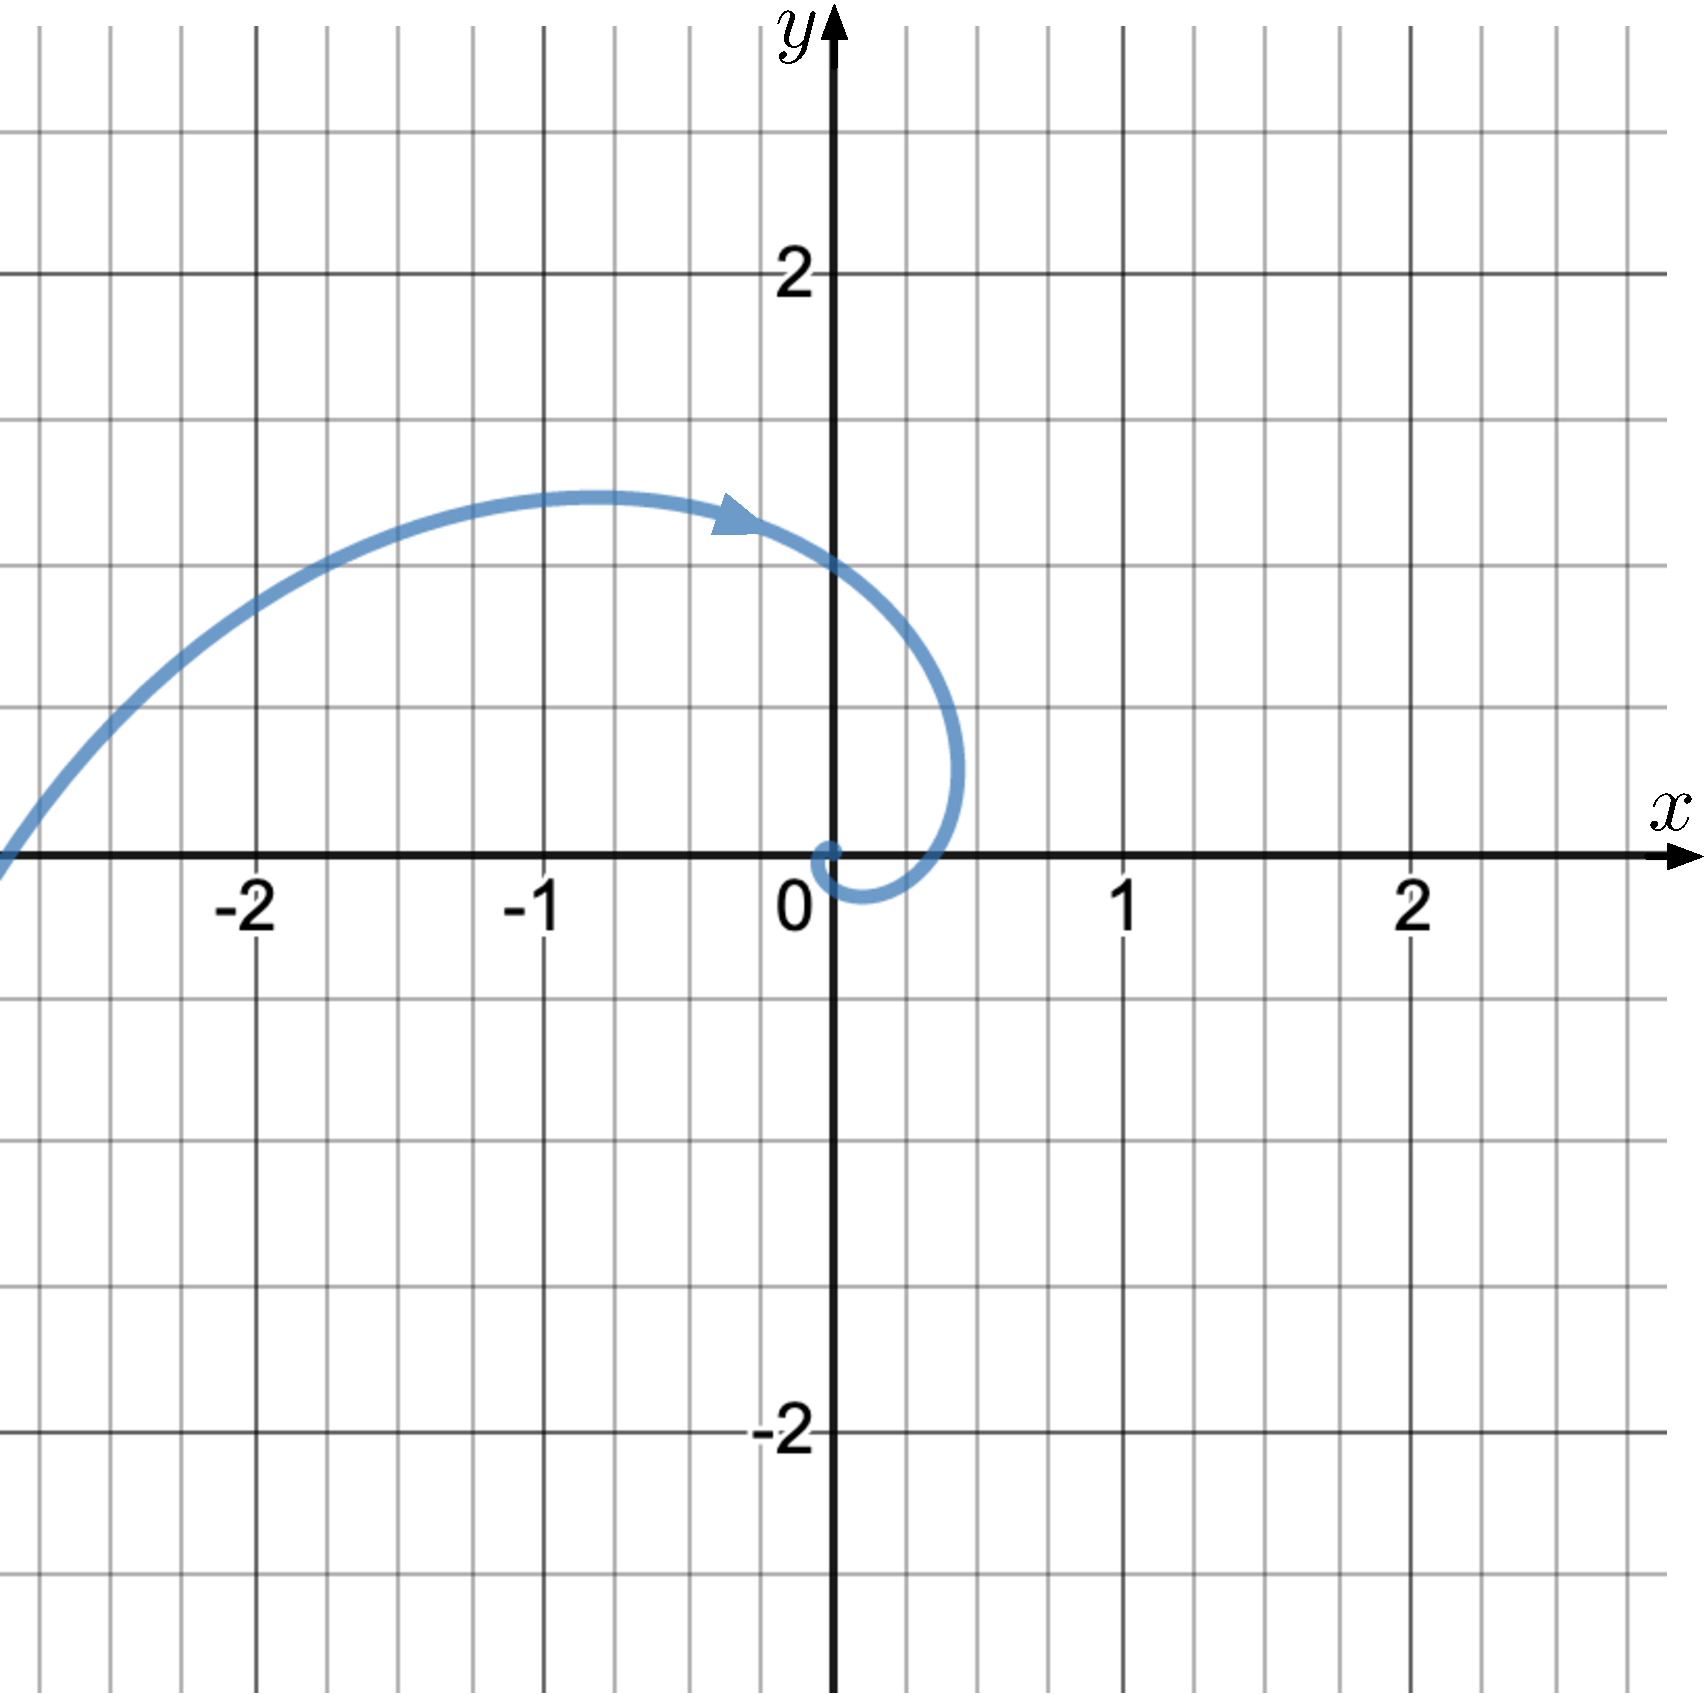
\includegraphics[height=200pt]{images/module18-spiral.pdf}
	\end{center}
	
	In this graph, we also include the graph for $t<0$. \\
	
	\item Let $c_1=-1$ and $c_2=0$ and we obtain
	$$ \vec{r}(t) = \begin{bmatrix}	 -\sin(3t) \\ -\cos(3t) \end{bmatrix} e^{-2t}$$	
	
	We add this graph to the previous one.
	\begin{center}
		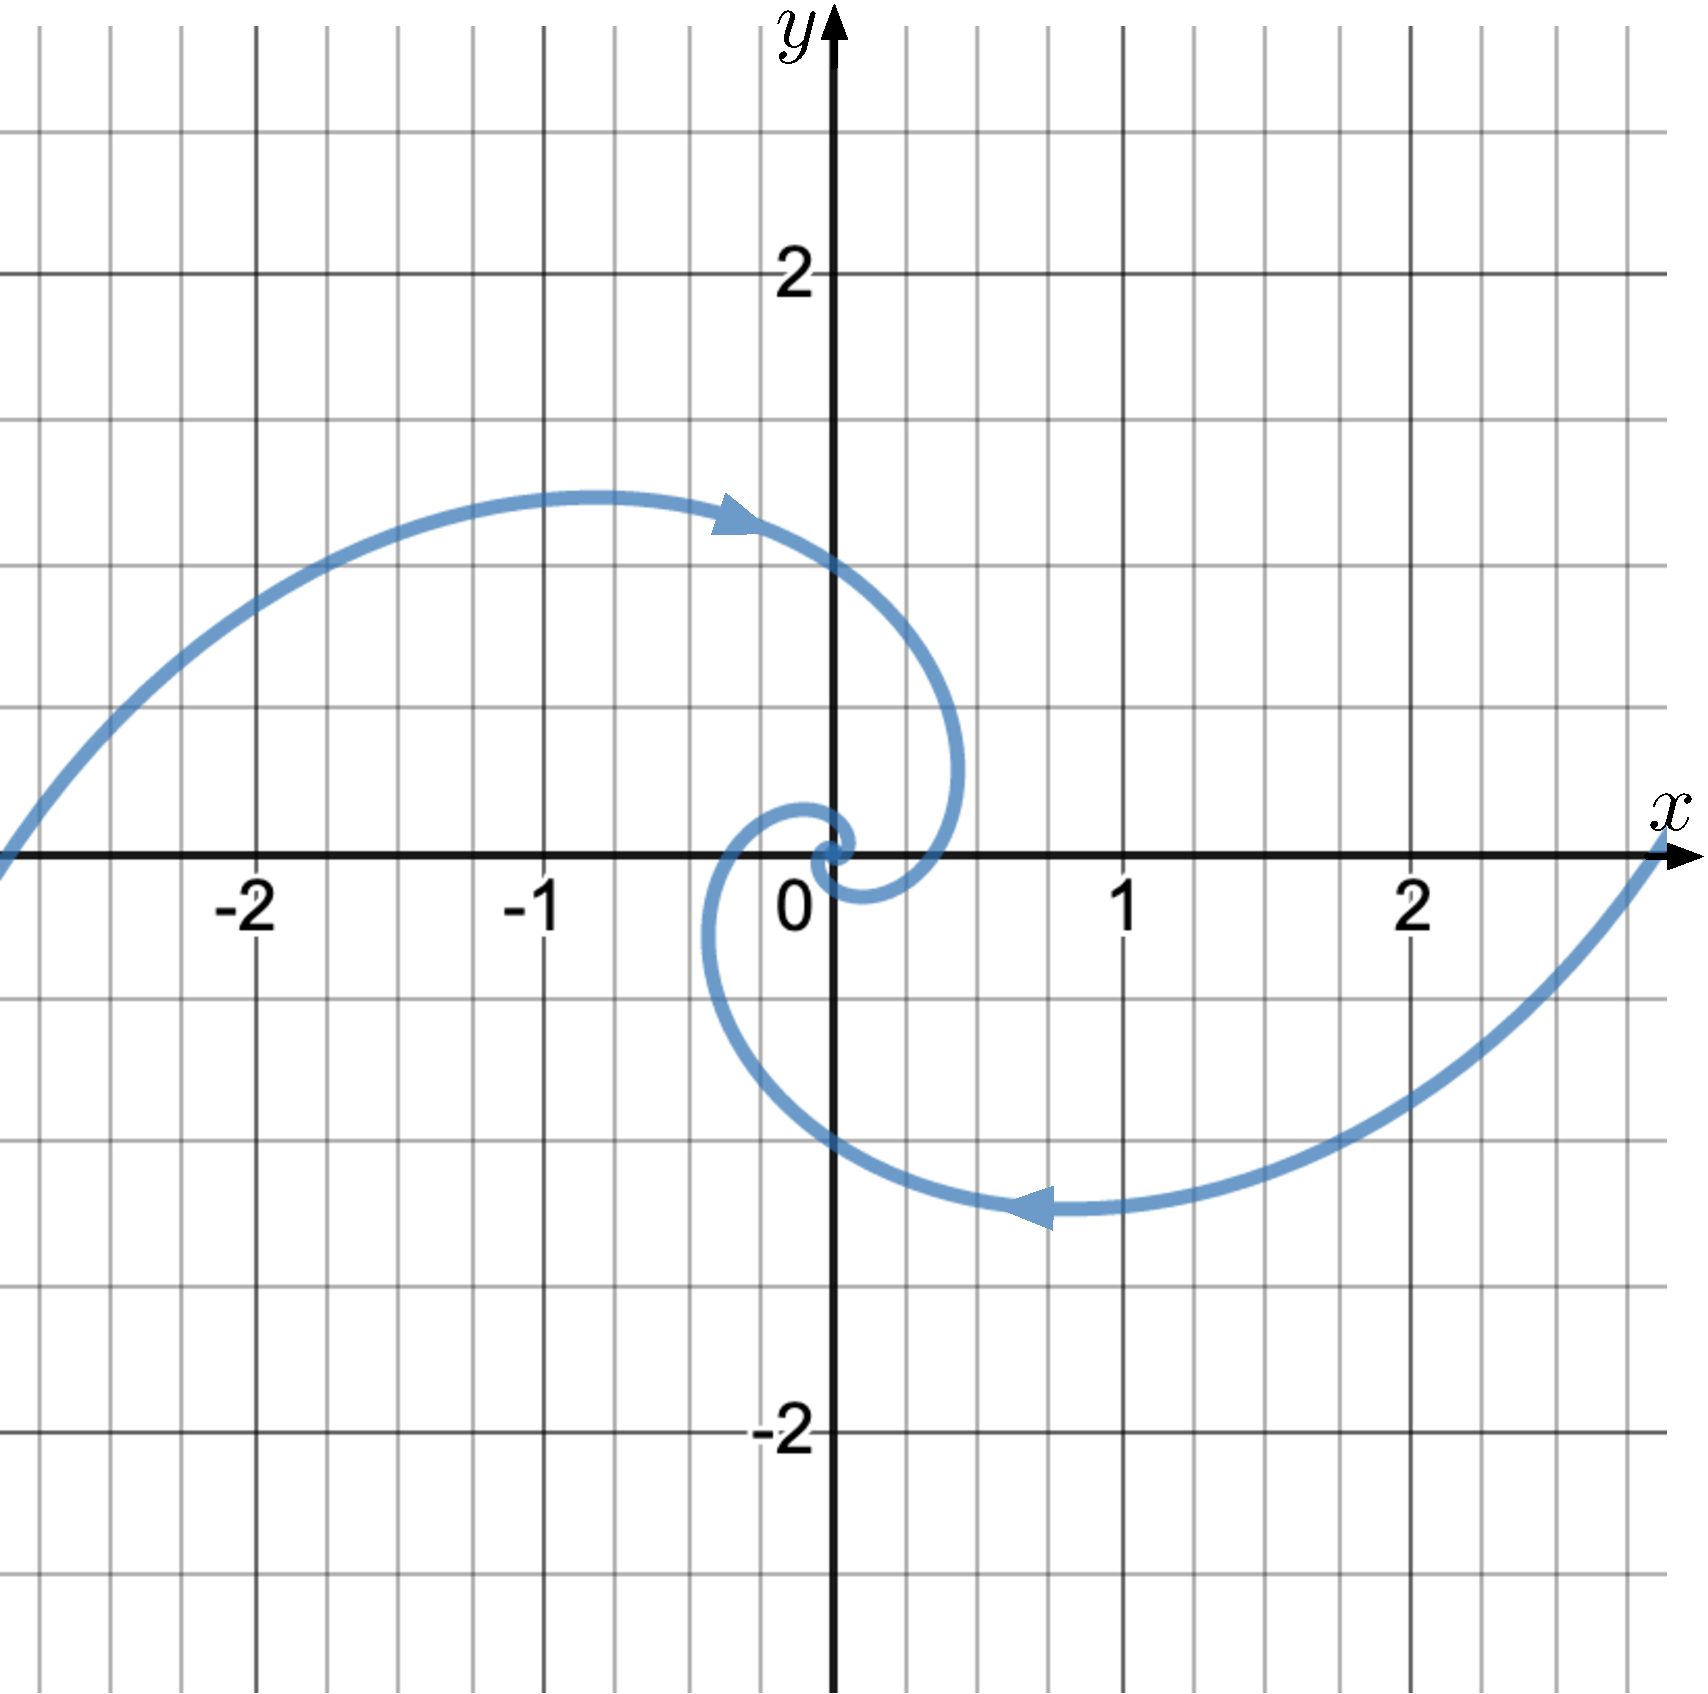
\includegraphics[height=200pt]{images/module18-spiral2.pdf}
	\end{center}
	
	\item Let $c_1=0$ and $c_2=\pm 1$ and we obtain
	$$ \vec{r}(t) = \begin{bmatrix}	 \mp \cos(3t) \\ \pm\sin(3t) \end{bmatrix} e^{-2t}.$$

	And add these to the graph:
	\begin{center}
		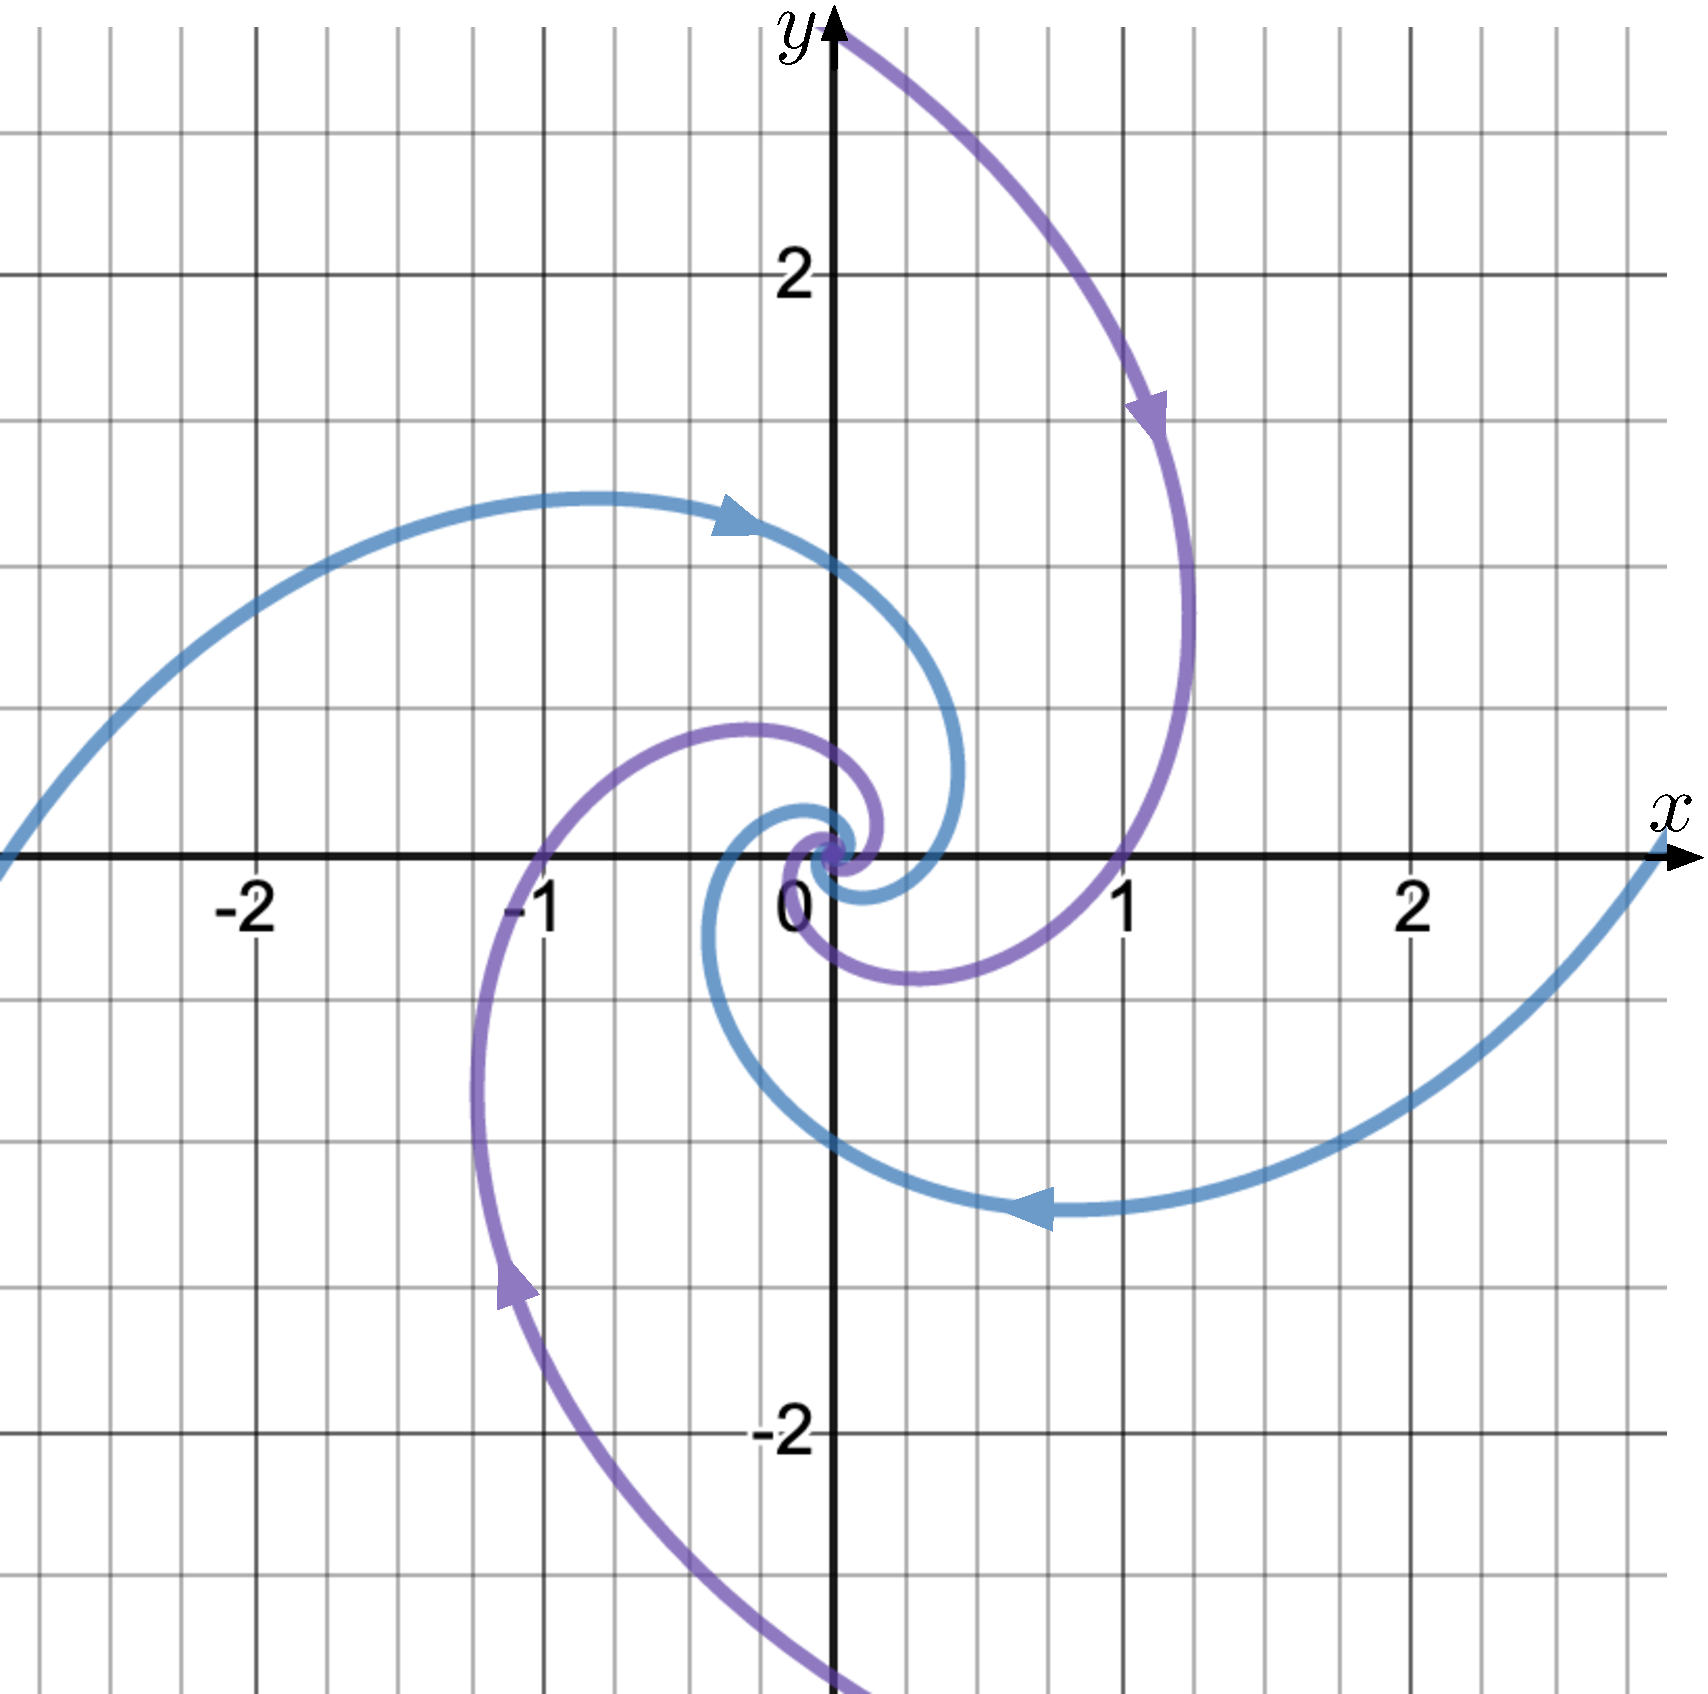
\includegraphics[height=200pt]{images/module18-spiral3.pdf}
	\end{center}

\end{itemize}

Sometimes, we need some solutions of the type $c_1=\pm 1$ and $c_2=\pm 1$ to get some different types of solutions, but we'll let you discover that on the core exercises.

These four solutions seem to give a good idea of all possible solutions: clockwise spirals converging to the origin.\\


Also observe that $\vec{r}(t) = \begin{bmatrix}0 \\ 0\end{bmatrix}$, so this system has an equilibrium solution.

This kind of equilibrium is called a \emph{spiral sink} and it is \emph{asymptotically stable}.
This means that it is a spiral and it converges to the equilibrium (the origin).
\end{example}





\begin{video}
	\begin{itemize}
		\item \qrvideo{https://youtu.be/nyI_JPDrJ_I}
		\item \qrvideo{https://youtu.be/dpbRUQ-5YWc}
	\end{itemize}
\end{video}





	\begin{exercises}

	\begin{problist}
	\prob For each matrix from practice problem \ref{mod16-gensol} from Module 16, sketch its phase portrait and label them as asymptotically stable or unstable. The system of ODEs is $\vec{r}'(t) = A \vec{r}(t)$ for the following matrices:
	\begin{enumerate}
	\begin{minipage}{.2\textwidth}
		\item $A = \begin{bmatrix} -7 & 6 \\ -9 & 8 \end{bmatrix}$;
		\item $A = \begin{bmatrix} 22 & 24 \\ -15 & -16\end{bmatrix}$;
		\item $A = \begin{bmatrix} 0 & 1 \\ -5 & 0 \end{bmatrix}$
		
		This is called a centre, which is stable, but not asymptotically stable. Can you tell why?
		\item $A = \begin{bmatrix} 0 & 1 \\ 5 & 0 \end{bmatrix}$;
		\item $A = \begin{bmatrix} 1 & \sqrt{3} \\ \sqrt{3} & -1\end{bmatrix}$;
		\item $A = \begin{bmatrix} 1 & \sqrt{3} \\ -\sqrt{3} & 1\end{bmatrix}$;
	\end{minipage}
	\qquad
	\begin{minipage}{.2\textwidth}
		\item $A = \begin{bmatrix} 0 & 1 \\ -4 & -4 \end{bmatrix}$
		
		This is called an improper node.
		\item $A = \begin{bmatrix} -4 & -6 \\ 2 & 3 \end{bmatrix}$;
		\item $A = \begin{bmatrix} 2 & -3 \\ 0 & 2 \end{bmatrix}$;
		\item $A = \begin{bmatrix} 2 & 0 \\ 0 & 2 \end{bmatrix}$;
		
		This is called a proper node.
		\item $A = \begin{bmatrix} 0 & 0 \\ 1 & 0\end{bmatrix}$; 
		\item $A = \begin{bmatrix} 0 & 0 \\ 0 & 1\end{bmatrix}$; 
	\end{minipage}
	\end{enumerate}
	
	\prob Consider a system of ODEs $\vec{r}'(t) = A \vec{r}(t)$.
	For each part, give an example of eigenvalues and eigenvectors of $A$ that would yield the required phase portrait:
	\begin{enumerate}
		\item Spiral sink (asymptotically stable);
		\item Spiral source (unstable);
		\item Centre (stable);
		\item Sink node (asymptotically stable);
		\item Source node (unstable);
		\item Saddle point (unstable);
		\item Improper node (stable);
		\item Improper node (unstable);
		\item Proper node (stable);
		\item Proper node (unstable);
	\end{enumerate}
	
	\prob Consider the system of ODEs
	$$
	\vec{r}'(t) = 
	\begin{bmatrix}
	1 & 1 \\ k & 1
	\end{bmatrix}\vec{r}(t).
	$$

	This system of ODEs changes behaviour depending on the parameter $k$.
	\begin{enumerate}
		\item Label the behaviour of the system for different values of $k$.
		\item We call the $k^\star$ the critical value of $k$ when the behaviour is different for $k<k^\star$ and for $k>k^\star$. For the critical value of $k$, sketch the phase portrait.
	\end{enumerate}
	
	
	\prob Consider the system of ODEs
	$$
	\vec{r}'(t) = 
	\begin{bmatrix}
	0 & 1 \\ -4 & -k
	\end{bmatrix}\vec{r}(t).
	$$

	This system of ODEs changes behaviour depending on the parameter $k$.
	\begin{enumerate}
		\item Label the behaviour of the system for different values of $k$.
		\item We call the $k^\star$ the critical value of $k$ when the behaviour is different for $k<k^\star$ and for $k>k^\star$. For the critical value of $k$, sketch the phase portrait.
		\item Which kinds of behaviours could be critical values?
	\end{enumerate}
	
	
	
	\prob Consider the system of ODEs
	$$
	\vec{r}'(t) = A \vec{r}(t).
	$$
	
	Let $T={\rm trace}(A) = a_{11}+a_{22}$, $D=\det(A) = a_{11}a_{22} - a_{12}a_{21}$, and $\Delta = T^2-4D$.
	
	\begin{enumerate}
		\item Show that the equilibrium solution is a saddle point if $D<0$.
		\item Show that the equilibrium solution is a spiral if $\Delta<0$ and $T\neq 0$.
		\item Show that the equilibrium solution is a centre if $T=0$ and $D>0$.
		\item When is the equilibrium point a node? \\

		\item Show that the equilibrium solution is asymptotically stable if $T<0$ and $D>0$.
		\item Show that the equilibrium solution is unstable if $T>0$ and $D<0$.
	\end{enumerate}






	\end{problist}
\end{exercises}

\end{module}



\begin{lesson}
	\Title{Phase Portraits}

	\Heading{Objectives}
	\begin{itemize}
		\item Bla
	\end{itemize}
	
	\Heading{Motivation} 

\end{lesson}




\newpage

\question
	Consider the following model for cheetah's and lions, where
	$$ \vec{p}(t) = \begin{bmatrix} \ell(t) = \text{population of lions} \\ c(t) = \text{population of cheetahs} \end{bmatrix} $$
	which satisfies
	$$
	\frac{d\,\vec{p}}{dt} = \begin{bmatrix}
 		1 & -1 \\
 		-3 & 1
 	\end{bmatrix}
	$$
	
	The general solution is:
	$$
	\vec{p}(t) = c_1 \begin{bmatrix} 1 \\ \sqrt{3} \end{bmatrix} e^{(1-\sqrt{3})t} + c_2 \begin{bmatrix} -1 \\ \sqrt{3} \end{bmatrix} e^{(1+\sqrt{3})t}.
	$$
\begin{parts}
	\item Without computing them, what are the eigenvalues and eigenvectors of the matrix?
	\item Sketch the graph of the solution with $c_1=\pm 1$ and $c_2=0$.
	\item Sketch the graph of the solution with $c_1=0$ and $c_2=\pm 1$.
	\item When one constant is set to 0, what is the shape of the graph? Is it always like that? Can you prove it?
	\item Sketch the graph of the solution with $c_1=\pm 1$ and $c_2=\pm 1$.
	\item Provide an interpretation of the different types of solutions.
\end{parts}

\begin{annotation}
	\begin{goals}
	At the end, let the students know that the equilibrium is called \emph{saddle point} and it is \emph{unstable}, because solutions go away from it.
	
	For the interpretation question, when one population hits zero, it is extinct, so the graph doesn't make sense. 
	
	We can interpret that if a population becomes extinct, then the other will behave as it would without competitors: grow exponentially fast!
	\end{goals}
\end{annotation}






\bookonlynewpage

\question
	Let us expand the model from the previous exercise to:
	$$ \vec{p}(t) = \begin{bmatrix} \ell(t) = \text{population of lions} \\ c(t) = \text{population of cheetahs} \end{bmatrix} $$
	which satisfies
	$$
	\frac{d\,\vec{p}}{dt} = \begin{bmatrix}
 		1 & -1 \\
 		-3 & 1
 	\end{bmatrix} \vec{p}
 	+ \begin{bmatrix}
 		- 10 \\ 50
	 \end{bmatrix} \vec{p}.
	$$
	
	The extra term corresponds to the effect of harvesting 10 lions and bringing in 50 cheetahs every year to the reserve. \\
	
	The general solution is:
	$$
	\vec{p}(t) = \begin{bmatrix} 20 \\ 10 \end{bmatrix} +
		c_1 \begin{bmatrix} 1 \\ \sqrt{3} \end{bmatrix} e^{(1-\sqrt{3})t} + c_2 \begin{bmatrix} -1 \\ \sqrt{3} \end{bmatrix} e^{(1+\sqrt{3})t}.
	$$
\begin{parts}
	\item Sketch the phase portrait.
	\item Provide an interpretation of the different types of solutions.
\end{parts}

\begin{annotation}
	\begin{goals}
		Some students might try to sketch everything from scratch.
		Remind them that the solutions look very similar and they only have to adapt the phase portrait they had before.
	\end{goals}
\end{annotation}



\bookonlynewpage


\question
	For each of the following general solutions, sketch the phase portrait.
\begin{parts}
	\item $	\vec{r}(t) = c_1 \begin{bmatrix} 2 \\ 1 \end{bmatrix} e^{2t} + c_2 \begin{bmatrix} -1 \\ 1 \end{bmatrix} e^{5t}.$
	\item $	\vec{r}(t) = c_1 \begin{bmatrix} 2 \\ 1 \end{bmatrix} e^{-2t} + c_2 \begin{bmatrix} -1 \\ 1 \end{bmatrix} e^{-5t}.$	
\end{parts}
\begin{annotation}
	\begin{goals}
	At the end, let the students know that these equilibria are called 
	\begin{itemize}
		\item \emph{source} and it is \emph{unstable}, because solutions go away from it.
		\item \emph{sink} and it is \emph{asymptotically stable}, because solutions converge to it.
	\end{itemize}
	
	If there is time, students can think about:

	Given a matrix $A$, which part of $A$ indicates whether the equilibrium is stable / unstable? Which part indicates whether it's a sink/source vs spiral sink/source?
	\end{goals}
\end{annotation}







%%%%%%%%%%%%%%%%%%%%%%%%%%%%%%
%
%  MODULE - Analysis of Systems
%
%%%%%%%%%%%%%%%%%%%%%%%%%%%%%%



\begin{module}{Analysis of Models with Systems}
	\label{sys:analysis}

	In this module you will learn
\begin{itemize}
	\item different ways to analyze models with several differential equations
\end{itemize}

\hfill \\



In this chapter, we have learned how to create models involving systems of ODEs and how to solve some special types of systems of ODEs.

Once we create a model that involves a system of ODEs, the ultimate goal is not to solve the system of ODEs, but to be able to understand how the situation will develop.
Solving the system of ODEs is often a large step in that direction, but it is more important to know how to interpret it in light of the original situation.

Sometimes, when we cannot find an explicit formula for the solution, it is still possible to study the system to find some properties and behaviours of the solutions. \\

In this module, we'll study one example using a few different methods.


\begin{example}
The goal here is not the modelling but the analysis of the model, so we will quickly explain the model. \\

We are going to model population versus cost of living in Toronto.


Consider the following functions
\begin{itemize}
\item $p(t) = $ Population of Toronto (GTA) in millions, $t$ years since the beginning of 2015.
\item $c(t) = $ Cost of living in Toronto (in thousands of dollars), $t$ years since the beginning of 2015.
\item Define a vector $\vec{x}(t) = \begin{bmatrix} p(t) \\ c(t) \end{bmatrix}$.
\end{itemize}

We assume that these two factors are related according to the following properties:
\begin{itemize}
\item In the absence of any migration, the population will decrease proportionally to the cost of living (with constant $a$);
\item There are always people moving into Toronto independently of its current population or cost of living (with constant $b$)
\item In the absence of any other factors, the cost of living; increases proportionally to the population (with constant $d$)
\item In the absence of any other factors, the cost of living; increases proportionally to the cost of living due to inflation (with constant $e$);
\item The city is always expanding, so the cost of living is always decreasing independently of its current population or cost of living (with constant $f$).
\end{itemize}
The constants $a,b,d,e,f$ are all positive. \\

Our model is:
$$
\vec{x}'(t) = 
	\begin{bmatrix}
 		0 & -a \\
 		d & e
	\end{bmatrix}
					\vec{x}(t) + 
	\begin{bmatrix}
		b \\ -f
	\end{bmatrix}
$$
\end{example}

\hfill

\begin{center}
\textbf{\color{cyan}
Qualitative evolution of quantities
}
\end{center}


%\paragraph{Qualitative evolution of quantities.}
We can try to figure out how these quantities, $p(t)$ and $c(t)$, are going to increase or decrease. \\

As an academic example, let us imagine that initially  \quad $p(0)=c(0)=0$.

Then, at $t=0$, we have
$$
p'(0)= b > 0 \quad \text{ and } \quad
c'(0)=-f < 0.
$$

This means that $p(t)$ is increasing while $c(t)$ wants to decrease.

Here we need to make sure that everything still makes sense: since it doesn't make sense to have a negative cost of living (government incentives to move into the city?!), we need to disregard our system and assume that $c(t)$ will continue constant while $c'(t)<0$.

We then have:
\begin{graybox}
\begin{center}
\begin{tabular}{c||c|c|c|c|c|c|c|c}
$\pmb{t}$	& $0$ 		& 			& &  			& 			& 	&	& \hspace{1cm} $+\infty$ \\[5pt] \hline\hline
$\pmb{p}$ & $0$	& $\nearrow$	& \hspace{0.5cm} &	\hspace{1cm}	&	&  \hspace{0.5cm}	&  	& 	\\[5pt] \hline
$\pmb{c}$ & $0$		& $\rightarrow$	&  0 & \hspace{1cm} & 	\hspace{0.5cm}	& \hspace{1cm} 	& \hspace{0.5cm}	&\hspace{1cm}	\\[5pt]
\end{tabular}
\end{center}
\end{graybox}

While $c(t)=0$, we have
$$
p'(t)= b > 0  \quad \text{ and } \quad 
c'(t)=d\, p(t) -f.
$$

This means that $p(t)$ is increasing with constant slope (linearly) until $c'(t_1)=0$.
We can figure out when this will happen:
$$
0=c'(t_1)=d\, p(t_1) -f \quad \Leftrightarrow \quad p(t_1) = \frac{f}{d}.
$$

So we continue our table:
\begin{graybox}
\begin{center}
\begin{tabular}{c||c|c|c|c|c|c|c|c}
$\pmb{t}$	& $0$ 		& 			& $t_1$ &  			& 			& 	&	& \hspace{1cm} $+\infty$ \\[5pt] \hline\hline
$\pmb{p}$ & $0$	& $\nearrow$	& $\displaystyle\frac{f}{d}$ &	\hspace{1cm}	&	&  \hspace{0.5cm}	&  	& 	\\[5pt] \hline
$\pmb{c}$ & $0$		& $\rightarrow$	&  0 & \hspace{1cm} & 	\hspace{0.5cm}	& \hspace{1cm} 	& \hspace{0.5cm}	&\hspace{1cm}	\\[5pt]
\end{tabular}
\end{center}
\end{graybox}

What happens after $t_1$?

Consider $t>t_1$ slightly after $t_1$. Then
$$
\begin{cases}
p'(t) = -a c(t) + b >0 & \text{ still positive because $c(t)$ is very small, but the slope is decreasing} \\
c'(t) = d p(t) + e c(t) - f	>0 & \text{ increasing quickly as both $p$ and $c$ increase}
\end{cases}
$$

\begin{graybox}
\begin{center}
\begin{tabular}{c||c|c|c|c|c|c|c|c}
$\pmb{t}$	& $0$ 		& 			& $t_1$ &  			& 			& 	&	& \hspace{1cm} $+\infty$ \\[5pt] \hline\hline
$\pmb{p}$ & $0$	& $\nearrow$	& $\displaystyle\frac{f}{d}$ &	\IncDown	&	&  \hspace{1cm}	&  	& 	\\[5pt] \hline
$\pmb{c}$ & $0$		& $\rightarrow$	&  0 & \IncUp & 	\hspace{0.5cm}	& \hspace{1cm} 	& \hspace{0.5cm}	&\hspace{1cm}	\\[5pt]
\end{tabular}
\end{center}
\end{graybox}

At a certain time $t_2$, the population will stop increasing. Let us find out when this happens:
$$
0=p'(t_2) = -a c(t_2) + b >0 
	\quad \Leftrightarrow \quad c(t_2) = \frac{b}{a}.
$$

\begin{graybox}
\begin{center}
\begin{tabular}{c||c|c|c|c|c|c|c|c}
$\pmb{t}$	& $0$ 		& 			& $t_1$ &  			& 	$t_2$		& 	&	& \hspace{1cm} $+\infty$ \\[5pt] \hline\hline
$\pmb{p}$ & $0$	& $\nearrow$	& $\displaystyle\frac{f}{d}$ &	\IncDown	& $\rightarrow$	&  \hspace{1cm}	&  	& 	\\[5pt] \hline
$\pmb{c}$ & $0$		& $\rightarrow$	&  0 & \IncUp & 	 $\displaystyle \frac{b}{a}$	& \hspace{1cm} 	& \hspace{0.5cm}	&\hspace{1cm}	\\[5pt]
\end{tabular}
\end{center}
\end{graybox}

After this point we have $t>t_2$ slightly after $t_2$:
$$
\begin{cases}
p'(t) = -a c(t) + b <0 & \text{ decreasing rapidly while $c'(t)>0$}\\
c'(t) = d p(t) + e c(t) - f	>0 & \text{ still increasing quickly until $p(t)=0$}
\end{cases}
$$

We expect that at some point $p(t_3)=0$. From that point on we have
$$
\begin{cases}
p'(t_3) = -a c(t_3) + b <0 & \text{ we need to ignore the model at this point and keep $p$ constant}\\
c'(t_3) = e c(t_3) - f	>0 & \text{ still increasing exponentially, as long as } c(t_3) > \frac{f}{e}
\end{cases}
$$

So this is our final table:
\begin{graybox}
\begin{center}
\begin{tabular}{c||c|c|c|c|c|c|c|c}
$\pmb{t}$	& $0$ 		& 			& $t_1$ &  			& 	$t_2$		& 	& $t_3$	& \hspace{1cm} $+\infty$ \\[5pt] \hline\hline
$\pmb{p}$ & $0$	& $\nearrow$	& $\displaystyle\frac{f}{d}$ &	\IncDown	& $\rightarrow$	&  \DecDown	& 0 	& $\rightarrow$	\\[5pt] \hline
$\pmb{c}$ & $0$		& $\rightarrow$	&  0 & \IncUp & 	 $\displaystyle \frac{b}{a}$	& \IncUp 	& 	& \IncUp	\\[5pt]
\end{tabular}
\end{center}
\end{graybox}



Observe that to do this analysis, we didn't need to know how to solve the system of ODEs. \\






\begin{center}
\textbf{\color{cyan}
Finding the equilibrium point(s)
}
\end{center}

%\paragraph{Finding the equilibrium point.} 
This is often easy to find, and by using the intuition we gained while learning to sketch phase portraits, this can give us a lot of insight about the solutions.

Let us find the equilibrium point:
$$
\begin{cases}
0= p'(t) = -a c(t) + b \\
0= c'(t) = d p(t) + e c(t) - f	
\end{cases}
\quad \Leftrightarrow \quad 
	\begin{cases}
 	\displaystyle c(t) = \frac{b}{a} \\[5pt]
	\displaystyle p(t) = \frac{af - be}{ad}
	\end{cases}
$$

Observe that if the population and cost of living are at these levels, then they will remain constant. \\

This also informs us that the disastrous scenario on the first analysis, where the population all left the city, might have been caused by the stating position. \\






\begin{center}
\textbf{\color{cyan}
Interpreting the phase portrait
}
\end{center}

We have seen in the last module how to sketch a phase portrait for a system of ODEs such as this one.

Let us assume that the constants $a=b=d=e=1$, $f=2$. Then the phase portrait is
\begin{center}
	\includegraphics*[width=250pt]{images/module18-pc.pdf}
\end{center}

Observe that both quantities should be positive, so let us focus on the quadrant where both are positive:
\begin{center}
	\includegraphics*[width=250pt]{images/module18-pc-closeup.pdf}
\end{center}

Observations:
\begin{itemize}
	\item Whenever a graph hits the axes, we must stop the model and re-evaluate what that means: when the graph hits the $c=0$ axis, then the population will start increasing until $c'>0 \Leftrightarrow p = 2$, so the graph will continue horizontally until the point $(2,0)$ where the model restarts.
	\item The population seems to converge to $0$ in all cases.
	\item The purple case seems to be an interesting one where the population and cost of living oscillate for a bit near the equilibrium and then the cost of living goes almost to zero before starting to go up again and forcing all the people to leave the city.
\end{itemize}



\hfill

\begin{center}
\textbf{\color{cyan}
Properties of the system
%Other questions about the system
}
\end{center}

%\paragraph{Other questions about the system.} 
We can look for other properties of the system of ODEs.

Based on the two analyses above, we can ask the following question:
\begin{itemize}
	\item Is there a value for the cost of living such that if it is above that, then eventually all the population will leave the city?
\end{itemize}

We know that 
$$
p'(t) = -a c(t) + b < 0 \quad \Leftrightarrow \quad c(t) > \frac{b}{a}.
$$

So as long as the cost of living is above $\frac{b}{a}$, then the population will continue to decrease. \\

Observe that depending on the constants $d, e, f$, we could still have
$$
c'(t) = d p(t) + e \frac{b}{a} - f < 0,
$$
so that we could end up with a cycle around the equilibrium we found before.









	\newpage 

\begin{exercises}

	\begin{problist}
	\prob Consider the model for student learning:
	\begin{itemize}
		\item $\vec{x} = \begin{bmatrix} x_1 \\ x_2 \end{bmatrix}$
		\item $x_1=$ student confidence in his/her own abilities ($x_1 \in [0,1]$)
		\item $x_2=$ student knowledge measured in IQ past 100
		\item $\vec{x}'(t) =
		\begin{bmatrix}
			a & b \\
			c & - d 
		\end{bmatrix}
		\vec{x}(t)
		+ \begin{bmatrix}
 			-e \\ 0
 		\end{bmatrix}$
		\item Constants $a,b,c,d,e>0$.
	\end{itemize}
	\begin{enumerate}
		\item What is the equilibrium solution $\vec{x}_e$? 
		\item If tests are harder, then $d$ is larger. How does that affect the equilibrium confidence and knowledge of students?
		\item Is the equilibrium solution stable?
		\item Assume $a=1, b=c=2, d=3,e=0$. As $t \to +\infty$, what are the possible outcomes for $\vec{x}(t)$ Explain the meaning for the students.
		\item Assume $a=1, b=c=2, d=3,e=0$. Some solutions satisfy $\displaystyle \lim_{t \to +\infty} \begin{bmatrix}c(t) \\ k(t) \end{bmatrix} = \begin{bmatrix} + \infty \\ + \infty \end{bmatrix}$.

			Show on a graph which initial conditions $\vec{x}(0) = \begin{bmatrix}c(0) \\ k(0) \end{bmatrix}$ guarantee this limit?

		\item If the tests become harder, i.e., $d$ increases, then is that good or bad for students?.
	\end{enumerate}
	
	\prob Consider the model for a tree:
	\begin{itemize}
		\item $\vec{x}(t) = \begin{bmatrix} \ell(t) \\ h(t) \end{bmatrix}$
		\item $\ell(t)=$ area of leafs on the tree
		\item $h(t)=$ height of the tree
		\item $\vec{x}'(t) =
		\begin{bmatrix}
			a & -b \\
			c & -d 
		\end{bmatrix}
		\vec{x}(t)$
		\item Constants $a,b,c,d>0$.
	\end{itemize}
	\begin{enumerate}
		\item Is it possible to have the tree growing taller and taller forever while the leaf area remains bounded?
		\item What would happen to the tree if the area of leafs is proportional to the height squared (not square root)?
		\item If $ad=bc$, explain what happens to the tree as $t\to \infty$.
	\end{enumerate}
	
	
	\prob Consider the model of a car:
	\begin{itemize}
		\item $\vec{c}(t) = \begin{bmatrix} v(t) \\ f(t) \end{bmatrix}$
		\item $v(t)=$ speed of the car
		\item $f(t)=$ amount of fuel in the car's tank
		\item $\vec{c}'(t) =
		\begin{bmatrix}
			-2 & 1 \\
			-2 & 0 
		\end{bmatrix}
		\vec{c}(t)
		+ \begin{bmatrix}
 			0 \\ -1	
		\end{bmatrix}$
	\end{itemize}
	\begin{enumerate}
		\item What is the equilibrium solution $\vec{c}_{\rm eq}$? What is the meaning of your result?
		\item If the car runs out of fuel at 300 m/s, then describe what happens to the car. 
		\item Describe what happens to the car when it starts at rest with a full tank of $300$ L.
		\item If the car attains its maximum velocity when there are still $300$ L of fuel left, what was the car's maximum velocity?


	\end{enumerate}


	\prob Consider the model for crying babies:
	\begin{itemize}
		\item $\vec{c}(t) = \begin{bmatrix} a(t) \\ b(t) \end{bmatrix}$
		\item $a(t)=$ volume of baby A's cries in dB
		\item $b(t)=$ volume of baby B's cries in dB
		\item $\vec{c}'(t) =
		\begin{bmatrix}
			-\alpha & \beta \\
			\beta & -\alpha 
		\end{bmatrix}
		\vec{c}(t)$
		\item constants $\alpha,\beta>0$.
	\end{itemize}

	The constants $\alpha$ and $\beta$ are $1$ and $2$. Does it make a difference which is 1 and which is 2?


	
		
	\end{problist}
\end{exercises}
\end{module}



\begin{lesson}
	\Title{Analysis of Models with Systems}

	\Heading{Objectives}
	\begin{itemize}
		\item Bla
	\end{itemize}
	
	\Heading{Motivation} 

\end{lesson}




\newpage

\question
	Consider the following model for cheetah's and lions, where



\bookonlynewpage












%%%%%%%%%%%%%%%%%%%%%%%%%%%%%%%%%%%%%%%%%%%%%%%%%%%%%%%%%%%%%%%%%%%%%%%%
%
%		Chapter 4 - Higher-Order Models
%
%%%%%%%%%%%%%%%%%%%%%%%%%%%%%%%%%%%%%%%%%%%%%%%%%%%%%%%%%%%%%%%%%%%%%%%%


%%%%%%%%%%%%%%%%%%%%%%%%%%%%%%%%%%%%%%%%%%%%%%%%%%%%%%%%%%%%%%%%%%%%%%%%
%
%		Chapter 4 - Higher-Order Models
%
%%%%%%%%%%%%%%%%%%%%%%%%%%%%%%%%%%%%%%%%%%%%%%%%%%%%%%%%%%%%%%%%%%%%%%%%


\begin{topic}[Higher-Order Models]



\vfil

\begin{center}
\begin{minipage}{500pt}
	\includegraphics*[width=500pt]{images/chap4-xkcd.png}

	\hfill {\footnotesize (image from \href{https://www.xkcd.com/226/}{xkcd - comic \#226})}
\end{minipage}
\end{center}


\end{topic}












%%%%%%%%%%%%%%%%%%%%%%%%%%%%%%
%
%  MODULE - Modelling with Second-Order ODEs
%
%%%%%%%%%%%%%%%%%%%%%%%%%%%%%%



\begin{module}{Modelling with Second-Order ODEs}
	\label{2nd:model}

	In this module you will learn
\begin{itemize}
	\item how to model physical phenomena to obtain second-order ODEs
\end{itemize}

\hfill \\


Whenever we model the movement of objects, we often find ourselves using \emph{Newton's Second Law of motion}:

\begin{definition}[Newton's Second Law of Motion]
	$F = m \cdot a$, \quad
	where $a$ is the acceleration of the object, $m$ is its mass, and $F$ is the net force acting on the object.
\end{definition}

Because this ``Law'' includes the acceleration of the object, and we know that
$$
{\rm acceleration} = a = \frac{d\,({\rm velocity})}{dt} = \frac{d\,v}{dt} = \frac{d^2 \, ({\rm position})}{dt^2} = \frac{d^2\,r}{dt^2},
$$
we will often end up with a Second-Order ODE.

Just like we did in module \ref{model-odes}, we will follow the step by step procedure developed in chapter 1.

\paragraph{\emph{Step 1.}} Define the problem

\begin{example}

\begin{minipage}{.75\textwidth}
We want to model the position of an object attached to the end of a spring. \\

The first step is to decide on what we want to find at the end of the process. 
So we define:
\begin{itemize}
	\item $y(t) =$ the vertical position of the mass, where $y=0$ is the position of the mass at rest.
\end{itemize}
\end{minipage}
\hfill
\begin{minipage}{44pt}
\includegraphics*[height=100pt]{images/module16-spring-mass-dashpot.pdf}	
\end{minipage}
\end{example}


\paragraph{\emph{Step 2.}} Build a mind map

\begin{example}
We start with the mass and then we brainstorm about the things that affect the mass:
\begin{center}
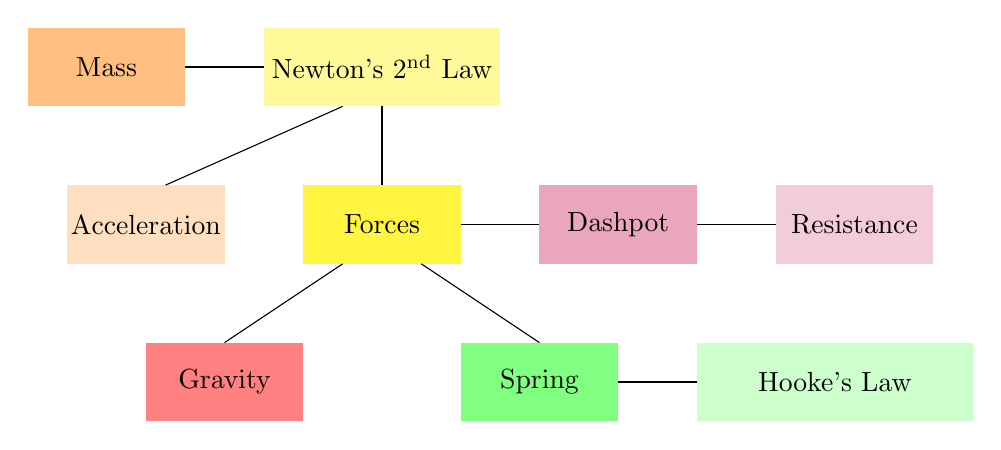
\begin{tikzpicture}
    \fill[color=orange!50!white] (-4.5,2) rectangle (-2.5,3) node[pos=.5] {\color{black}Mass};
%    \draw (-3.5,2) -- (-3.25,1);
    \fill[color=orange!25!white] (-4,1) rectangle (-2,0) node[pos=.5] {\color{black}Acceleration};
    \draw (-0.5,2) -- (-2.75,1);
    \draw (-2.5,2.5) -- (-1.5,2.5);
    \fill[color=yellow!40!white] (-1.5,2) rectangle (1.5,3) node[pos=.5] {\color{black}Newton's $2^{\rm nd}$ Law};
    \draw (0,1) -- (0,2);
  \fill[color=yellow!75!white] (-1,0) rectangle (1,1) node[pos=.5] {\color{black}Forces};
    \draw (-0.5,0) -- (-2,-1);
    \fill[color=red!50!white] (-1,-1) rectangle (-3,-2) node[pos=.5] {\color{black}Gravity};
    \draw (0.5,0) -- (2,-1);
    \fill[color=green!50!white] (3,-2) rectangle (1,-1) node[pos=.5] {\color{black}Spring};
    \draw (3,-1.5) -- (4,-1.5);
    \fill[color=green!20!white] (4,-2) rectangle (7.5,-1) node[pos=.5] {\color{black}Hooke's Law};
    \draw (1,0.5) -- (2,0.5);
    \fill[color=purple!35!white] (2,0) rectangle (4,1) node[pos=.5] {\color{black}Dashpot};  
    \draw (4,0.5) -- (5,0.5);
    \fill[color=purple!20!white] (5,0) rectangle (7,1) node[pos=.5] {\color{black}Resistance};  
\end{tikzpicture}
\end{center}
	
\end{example}


\paragraph{\emph{Step 3.}} Make assumptions

\begin{example}
In this step, we discuss the mind map we created and how we plan to address each of the boxes, or only some of the boxes. This will involve making assumptions and providing an explanation to the assumptions we make.

\begin{enumerate}
	\item As we described before the example, the plan is to use Newton's Second Law of Motion to describe the motion of the mass. This involves three quantities:
	\begin{itemize}
		\item mass: we assume that this is known to the modeller;
		\item acceleration: as we mentioned above, this is directly related to the position of the object. We have $y''(t)=$ acceleration, as long as we are assuming that the object is moving only vertically;
		\item forces: we need to find all the forces acting on the object and add them.
	\end{itemize}
\end{enumerate}

The forces acting on the object need to be discussed separately:
\begin{itemize}
	\item Gravity: we will go on a limb here and say that the force of the spring is much larger, so we will ignore this force;
	\item Spring: the force of the spring that acts on the mass follows Hooke's Law that says that the force is proportional to the extension/contraction of the spring. The constant of proportionality depends on the spring and we assume that it is known;
	\item Dashpot: the dashpot provides resistance. We will assume that it provides linear resistance to movement: the force is proportional to the velocity, with a proportionality constant that depends on the dashpot and is assumed to be known to the modeller.
\end{itemize}
	
\end{example}


\paragraph{\emph{Step 4.}} Construct a model

\begin{example}
We will start with Newton's Second Law of motion:
\begin{itemize}
	\item $m y''(t) = F(t)$ \\
\end{itemize}

and we will  add the different forces one by one:
\begin{itemize}
	\item Spring: the force of the spring is \quad $- k y(t)$; \hfill (you should check that the sign makes sense)
	\item Dashpot: the force of the dashpot is \quad $- \gamma y'(t)$. \hfill (you should also check the sign of this term) \\
\end{itemize}

Right now we have the following model:
$$
m y''(t) = -ky(t) - \gamma y'(t).
$$

\end{example}



\paragraph{\emph{Step 5.}} Model assessment

We'll skip this part here, but you should try to develop some tests to check the validity of the model we came up with.
Specifically, the fact that we ignored gravity should be checked to make sure that it doesn't affect our model too much.

\paragraph{\emph{Step 6.}} Putting it all together in a report

We'll skip this part here.





	\newpage

\begin{exercises}

	\begin{problist}
	
	\prob Consider a mountain with shape $y=f(x)$ a hiker who is climbing down the mountain with horizontal position $x(t)$. She starts at a peak of the mountain at $x_0=0$. As she climbs down the mountain, she notices that from her point-of-view, the rate of change of the slope of the mountain is decreasing linearly with time.
		The hiker also notices that her horizontal speed is constant.
	
		Model the hiker's position and the shape of the mountain.
	
	\prob 
	
	\begin{center}
		\includegraphics*[width=150pt]{images/module20-catenary.pdf}
	\end{center}

	\prob Model a ping pong ball travelling through the air.
	
	\begin{center}
		\includegraphics*[height=100pt]{images/module20-hotairballoon.pdf}
	\end{center}
	
	\prob Model an old TV floating or sinking in the ocean.
	
	\prob Model a container floating in the ocean with a leak that allows water to get inside.
	
	\prob Model a hot air balloon flying through the air.
	
	\prob Model the shape of a rope hanging between two poles.

	\begin{center}
		\includegraphics*[width=150pt]{images/module20-suspensionbridge.pdf}
	\end{center}

	\prob Model the shape of the cables of a suspension bridge.
	
	\prob Imagine a cylinder floating vertically partially submerged in a lake. Model the position of its top.
	
	\prob Model a ball rolling down a hill.
	
	\prob Model an electric circuit with a resistor, and inductor, and a capacitor in series.
	
	\prob Start with the Law of Conservation of Energy and assume a conservative force. Then show that you obtain Newton's Second Law of motion.
	
	\end{problist}
\end{exercises}

\end{module}



\begin{lesson}
	\Title{Modelling with Second-Order ODEs I}

\Heading{Textbook}
	\begin{itemize}
		\item Module 19
	\end{itemize}

\Heading{Objectives}
	\begin{itemize}
		\item Model physical phenomena to obtain a second-order ODE
		\item Understand how to use Newton's Second Law of Motion
		\item Follow the step-by-step procedure to create a model
	\end{itemize}
	
\Heading{Motivation} 

By this point, the students should have a good idea on how the modelling task goes.

Models about moving objects often require Newton's Second Law of Motion which end up having the form of a second-order ODE.

Engineering and Physics students will find models like this often in their studies.



\Heading{Preparation for Class}
\begin{itemize}
	\item Read textbook
	\item Read the core exercise \ref{2nd:keyboard} and solve steps 1 (define problem), 2 (create a mind map), and 3 (make assumptions)
\end{itemize}




\Heading{Tutorials and Projects}
\begin{itemize}
	\item Project \ref{proj:pursuit}: \pursuittitle
	\item Project \ref{proj:spring}: \springtitle
\end{itemize}




\end{lesson}




\question \label{2nd:keyboard}
	Here are some facts about laptop keys:

\begin{itemize}
\begin{minipage}{.4\textwidth}
\item[\color{Gray}(da)] Each key must also include some damping, so that it doesn't keep oscillating back and forth once pressed.

\item[\color{Gray}(di)] A typical letter key is 15mm$\times$15mm and when pressed has a maximum displacement of 0.5mm.

\item[\color{Gray}(fo)] On average, a person exerts the force of $42\,$N with one finger on a key.
\end{minipage}
\hfill
\begin{minipage}{.4\textwidth}
\item[\color{Gray}(gr)] Gravity is much weaker than the spring that keeps the key in place.

\item[\color{Gray}(hl)] Each key has a spring to make the key return to its original position after being pressed (Hooke's Law: ``the force is proportional to the extension'').

\item[\color{Gray}(lo)] Keys last 50 million presses on average.

\item[\color{Gray}(ve)] Keys can only move vertically.
\end{minipage}
\end{itemize}
	
\begin{annotation}
	\begin{goals}
		.1 should be very quick, since a very (very) similar example was solved in the module.
	\end{goals}
\end{annotation}
\begin{parts}
	\item Model a laptop keypress.
	\item What happens if the damping system of the key is broken? What happens if the damping system is too strong? How strong should the damping system be?
	\item What happens to the key when the spring breaks?
\end{parts}





\bookonlynewpage

\begin{lesson}
	\Title{Modelling with Second-Order ODEs II}

\Heading{Textbook}
	\begin{itemize}
		\item Module 19
	\end{itemize}
	
\Heading{Objectives}
	\begin{itemize}
		\item Model physical phenomena to obtain a second-order ODE
		\item Understand how to use Newton's Second Law of Motion
		\item Follow the step-by-step procedure to create a model
	\end{itemize}
	
\Heading{Motivation} 

This class, students work on a model that involves a bit more of Linear Algebra (projections) and some ``uglier'' expressions.


\Heading{Preparation for Class}
\begin{itemize}
	\item Read textbook
	\item Read the core exercise \ref{2nd:ballrolling} and solve steps 1 (define problem), 2 (create a mind map), and 3 (make assumptions)
\end{itemize}

\Heading{Tutorials and Projects}
\begin{itemize}
	\item Project \ref{proj:pursuit}: \pursuittitle
	\item Project \ref{proj:spring}: \springtitle
\end{itemize}


\end{lesson}


\begin{annotation}
	\begin{goals}
		\Goal{Ball rolling}
		Different approach depending on students. \\
		
		\emph{Students need some challenge and have time}:
		\begin{itemize}
			\item Ramp $y=f(x)$ makes it simpler
			\item Need projection (Linear Algebra) to find gravity force along the ramp at $(x_0,y_0) = \big(x_0,f(x_0)\big)$:
			$$			
			\ell = (0,-mg) \cdot (1, k)\frac{1}{\sqrt{1+k^2}} = -\frac{mgk}{\sqrt{1+k^2}}
			$$
			where $k = f'(x_0)$.
			So gravity force along the ramp is:
			$$
			\vec{F}_g = \ell (1, k)\frac{1}{\sqrt{1+k^2}} = -\frac{mgk}{1+k^2} (1,k)
			$$
			\item Yields second-order ODE 
		\end{itemize}
		\hfil
		
		\emph{Weaker students with less time}:
		\begin{itemize}
			\item Give the formula for gravity force along the ramp:
			$$
			\vec{F}_g = \ell (1, k)\frac{1}{\sqrt{1+k^2}} = -\frac{mgk}{1+k^2} (1,k)
			$$
		\end{itemize}
		
		\hfil
		
		\emph{Follow-up question}:
		\begin{itemize}
			\item Ramp is $y=(x-1)^2$
			\item Get second-order ODE for ball position
			\item Will the ball always move to the right? Justify with the ODE.
			\item Approximate near the bottom of the ramp: $y' \approx 0 \Leftrightarrow \sqrt{1+(y')^2} \approx 1$ and solve the simpler ODE.
			\item When is this approximation valid? (when ball oscillates back and forth near the bottom)
		\end{itemize}
	\end{goals}
\end{annotation}
\question \label{2nd:ballrolling}
	Model a ball rolling down a ramp.

	



\standardonlynewpage

%%%%%%%%%%%%%%%%%%%%%%%%%%%%%%
%
%  MODULE - Second-Order Linear ODEs with Constant Coefficients
%
%%%%%%%%%%%%%%%%%%%%%%%%%%%%%%



\begin{module}{Second-Order Linear ODEs with Constant Coefficients}
	\label{2nd:solving}

	In this module you will learn
\begin{itemize}
	\item how to solve this type of ODEs
\end{itemize}

\hfill \\

In this module we will learn how to solve a specific type of Second-Order ODEs: linear second-order ODEs with constant coefficients. These equations have the form
$$
a y''(t)  + b y'(t) + c y(t) = f(t).
$$

\subsection{Homogeneous ODEs}

These are ODEs above with $f(t) \equiv 0$.
So we are trying to solve
$$
a y''(t)  + b y'(t) + c y(t) = 0.
$$

The main idea to solve these problems is the same as for systems: making an \emph{educated guess} that the solution should look like an exponential:
$$
y(t) = e^{rt},
$$
and we need to find which values of $r$ yield solutions.

We do that by plugging this formula for $y(t)$ into the ODE:
\begin{itemize}
	\item $y'(t) = r e^{rt}$
	\item $y''(t) = r^2 e^{rt}$
\end{itemize}

We get
$$
a r^2 e^{rt} + br e^{rt} + c e^{rt} = 0
\quad \Leftrightarrow \quad 
	a r^2 + br + c = 0.
$$

This equation for $r$ is called the \emph{characteristic equation}.

We know how to solve it:
$$
r = \frac{-b \pm \sqrt{b^2-4ac}}{2a}.
$$

That means that we have three possible cases.





\paragraph{\color{cyan}Two real distinct roots.} When $b^2-4ac > 0$, we have two possible values for $r$ that are real numbers: $r_1$ and $r_2$.

Then, similarly to what we did with systems of ODEs, we obtain two solutions
$$
y_1(t) = e^{r_1 t} \quad \text{ and } \quad y_2(t) = e^{r_2 t},
$$
and the general solution is
$$
y(t) = c_1 e^{r_1 t} + c_2 e^{r_2 t}.
$$

\begin{video}
\begin{itemize}
	\item \qrvideo{https://youtu.be/_8fcT95JV34}
	\item \qrvideo{https://youtu.be/nE_OnX8ulHA}
	\item \qrvideo{https://youtu.be/v1xKZOrGsVc}
\end{itemize}	
\end{video}



\paragraph{\color{cyan}Two complex roots.} When $b^2-4ac<0$, we have two possible values for $r$, but they are complex values:
$$
r_{\pm} = \alpha \pm i\beta.
$$
\begin{graybox}
What are the value of $\alpha$ and $\beta$?	
\end{graybox}

Then we have two solutions
$$
y_{+}(t) = e^{(\alpha+i\beta) t} \quad \text{ and } \quad y_{-}(t) = e^{(\alpha-i\beta) t},
$$
and the general solution is
$$
y(t) = a_1 e^{(\alpha+i\beta) t}  + a_2 e^{(\alpha-i\beta) t}.
$$

Just like we did with systems with complex eigenvalues, we prefer to write the solutions without complex numbers, so we expand it using Euler's formula to get
\begin{align*}
y(t) 	& = a_1 e^{(\alpha+i\beta) t}  + a_2 e^{(\alpha-i\beta) t} \\
		& = a_1 e^{\alpha t}e^{i\beta t}  + a_2 e^{\alpha t}e^{-i\beta t} \\
		& = a_1 e^{\alpha t} \big( \cos(\beta t) + i \sin(\beta t) \big)  + a_2 e^{\alpha t} \big( \cos(\beta t) - i \sin(\beta t) \big) \\
		& = (a_1+a_2)  \cos(\beta t)e^{\alpha t} + i (a_1-a_2)\sin(\beta t) e^{a\alpha t} \\
		& = c_1 \cos(\beta t)e^{\alpha t} + c_2\sin(\beta t) e^{\alpha t}
\end{align*}

\begin{graybox}
How do $c_1$ and $c_2$ depend on $a_1,a_2$?	
\end{graybox}

So another way to write the general solution is
$$
y(t) = c_1 \cos(\beta t)e^{\alpha t} + c_2\sin(\beta t) e^{\alpha t}.
$$


\begin{video}
\begin{itemize}
	\item \qrvideo{https://youtu.be/DORl6GMPtjM?t=396}
\end{itemize}	
\end{video}




\paragraph{\color{cyan}One real repeated root.} When $b^2-4ac=0$, then we are left with only one value for $r=-\frac{b}{2a}$.

We then have one solution
$$
y_1(t) = e^{-\frac{b}{2a}t}.
$$

\begin{example}
Consider the ODE 
$$
y''(t) + 2y'(t) + y(t) = 0.
$$	

To find the general solution, we assume that the solutions have the form $y(t) = e^{rt}$, which means that $r$ must satisfy
$$
r^2 +2r+1 = 0 
	\quad \Leftrightarrow \quad r=-1,
$$
so $y_1(t) = c_1 e^{-t}$.

Now can we solve this ODE with the following initial conditions?
\begin{itemize}
	\item $y(0)=2$ and $y'(0)=-2$.
	\item $y(0)=2$ and $y'(0)=1$.
\end{itemize}
\end{example}

This previous example, should give a good idea on why having one value for $r$ means that we are missing something. 
We need to find a second solution $y_2(t)$. \\


\begin{graybox}
If we want to find all the divisors of $42$, and we already know that $d_1=2$ is a divisor, then we can use the divisor $d_1$ we know to write 
$$
d_1 \cdot x = 42 
	\quad \Leftrightarrow\quad 2x = 42
	\quad \Leftrightarrow\quad x = 21,
$$
where $x$ is the product of all the other divisors.

We used the divisor we knew $d_1$ to obtain a simpler problem for the other divisors.
\end{graybox}


\subparagraph{\color{cyan}Reduction of Order.} The idea here is the same. We use the solution we found to try to obtain a simpler ODE for the other solution:
$$
y(t) = y_1(t) \cdot u(t),
$$
where $y(t)$ is the solution we are still missing, $y_1(t)$ is the solution we already found, and $u(t)$ is a function. If we find $u(t)$, then we find $y(t)$. We hope that the function $u(t)$ satisfies a simpler problem.

To do that, we need to plug the formula above for $y(t)$ into the original ODE. 

\begin{important}
You should do these calculations yourself.
Remember to use the product rule and to be careful not to make any mistakes.	

Also remember that we know the value of $r$.
\end{important}

We obtain
$$
u''(t) = 0
\quad \Leftrightarrow \quad u(t) = c_1 + c_2 t.
$$

This means that we found 
$$
y(t) = (c_1 + c_2 t) e^{rt}
\quad \Leftrightarrow \quad y(t) = \underbrace{c_1 e^{rt}}_{\substack{\rm previous \\ \text{solution } y_1(t)}} + c_2 t e^{rt}.
$$

The general solution is 
$$
y(t) = c_1 e^{rt} + c_2 t e^{rt},
$$
where $r = -\frac{b}{2a}$.


\begin{video}
\begin{itemize}
	\item \qrvideo{https://youtu.be/DORl6GMPtjM}
\end{itemize}	
\end{video}






\subsection{Non-Homogeneous ODEs}

We are trying to solve
\begin{equation}\tag{$\star$}\label{mod20:orig}
a y''(t)  + b y'(t) + c y(t) = f(t),
\end{equation}
where $f(t)$ is a known function. \\


\begin{important}
If $u(t)$ is the general solution of
\begin{equation}\tag{$H$}\label{mod20:hom}
ay''(t)+by'(t)+cy(t) = 0,
\end{equation}
and $v(t)$ satisfies
\begin{equation}\tag{\ref{mod20:orig}}
ay''(t)+by'(t)+cy(t) = f(t),
\end{equation}
then $y(t) = u(t) + v(t)$ gives the general solution of
$$
ay''(t)+by'(t)+cy(t) = f(t).
$$

This is a practice problem at the end of this module.
\end{important}


This means that to solve this ODE, we split the general solution into two parts
$$
y(t) = y_c(t) + y_p(t),
$$
where
\begin{itemize}
	\item $y_c(t)$ is called the \emph{complementary solution} and it is the general solution of the corresponding homogenous ODE \eqref{mod20:hom}. It is solved using the technique we studied above.
	\item $y_p(t)$ is called the \emph{particular solution} and it is one function that satisfies the original ODE \eqref{mod20:orig}.
\end{itemize}

\begin{important}
It may seem strange that to solve the original ODE, we need its solution, but what we are trying to do is find \emph{all possible solutions} of the original ODE.

To find all possible solutions of the original ODE, we require two things:
\begin{itemize}
	\item \emph{One} solution of the original ODE:  $y_p(t)$,
	\item and all possible solutions of the homogeneous ODE: $y_c(t)$.
\end{itemize}
\end{important}


We already know how to find the complementary solution, so we will focus our attention on finding one particular solution.

\paragraph{\color{cyan}Method of Undetermined Coefficients.} As you probably have gotten used to by now, this is a method of educated guess-and-check. \\

Let us look at the equation from a different point-of-view
\begin{align*}
a y''(t) + by'(t) + cy(t) & = f(t) \\
\substack{\displaystyle\text{linear combination of}\\\displaystyle\text{function and derivatives}} & = f(t)
\end{align*}
and remember that some functions don't change much when differentiated:
\begin{itemize}
	\item Exponentials $y=ce^{rt}$ don't change their form after differentiation $y'=cre^{rt} = de^{rt}$. They even keep the same exponential term.
	\item Polynomials don't change their form either: their derivative is also a polynomial, with lower degree.
	\item Cosines and Sines alternate between one and the other, so functions of the form $y=c_1 \sin(rt) + c_2\cos(rt)$ don't change after differentiation.
\end{itemize}


\begin{important}
This means that, if $f(t)$ is one of these types of function, then $y(t)$ must be of the same form.	
\end{important}

\begin{example}
Find a particular solution for the ODE
$$
y''  - 4y = 10 e^{3t} = (\text{constant}) \cdot (\text{exponential of } 3t).
$$	

Our candidate is
$$
y_p(t) = A e^{3t}.
$$

Now we need to find the constant $A$ by plugging it into the ODE:
$$
9 A e^{3t} - 4 \cdot A e^{3t} = 10 e^{3t}
\quad \Leftrightarrow \quad 
	A = 2,
$$
so $y_p(t) = 2 e^{3t}$ is a particular solution.
\end{example}


\begin{example}
Find a particular solution for the ODE
$$
y''  - 4y = 3t^2+2t = (\text{polynomial of degree 2}).
$$	

Our candidate is
$$
y_p(t) = At^2 + Bt + C.
$$

Now we need to find the constants $A, B, C$ by plugging the formula for $y_p$ into the ODE:
$$
2A - 4At^2 - 4B t - 4C = 3t^2+2t
\quad \Leftrightarrow \quad 
\begin{cases}
A = -\frac34 \\
B = -\frac12 \\
C = \frac{A}{2} = -\frac38.	
\end{cases}
$$
so $y_p(t) = -\frac34 t^2 - \frac{t}{2} - \frac38$ is a particular solution.
\end{example}

There are some more details to deal with when using this method that will be addressed in the core exercises.




\begin{video}
\begin{itemize}
	\item \qrvideo{https://youtu.be/CjZ0TfPnWVU}
	\item \qrvideo{https://youtu.be/ubdSxJ2nmVk}
	\item \qrvideo{https://youtu.be/YRvqem1n0nQ}
\end{itemize}	
\end{video}





	\begin{exercises}

	\begin{problist}

	\prob Find the complementary and particular solutions for the following ODEs
	\begin{enumerate}
		\item $y''-2y'-3y=3e^{2t}$
		\item $y''-2y'-3y=-3te^{-t}$
		\item $y''-9y=t^2e^{-3t}-6$
		\item $y''+2y'-8y=e^{-t}-2e^t$
		\item $y''-y'-6y=\sin(t)$
		\item $y''-y'-6y=\sin(t)+3e^{3t}$
		\item $y''+4y=(2t+1)\sin(t) + 4\cos(2t)$
		\item $y''+y=\cos(2t)+t^3$
		\item $y''-y'-2y=t\cos(t) - t\sin(t)$
		\item $y''+5y'+6y = 2e^{-2t}$
	\end{enumerate}



	\prob What is the form of the particular solution for the ODE
	\begin{multline*}
		y^{(6)} + y^{(5)} -5 y^{(4)} + 31 y'''-176y''+220y' \\
			= (3t-1)e^{2t} + t^3e^{-5t}\sin(3t) + (4t^2-2t) e^{-2t} \sin(3t),
	\end{multline*}
	knowing that 
	\begin{multline*}
		x^6 + x^5 - 5 x^4 + 31 x^3 - 176 x^2 + 220 x \\
			= \big((x^2+2)+9\big)*(x-2)^2*x*(x+5)\quad ?
	\end{multline*}

	\prob What is the form of the particular solution for the ODE
	\begin{multline*}
		y'''' - 4 y''' + 10y'' - 12 y' + 5y \\
			= t e^t + t^2 \cos(2t) - (2t+1) e^t \sin(t),
	\end{multline*}
	knowing that 
	\begin{multline*}
		x^4 - 4x^3 + 10 x^2 - 12 x + 5 \\
			= (x-1)^2 \big( (x-1)^2+4\big)\quad  ?
	\end{multline*}

	\prob Consider the ODE
	$$
	t^2 y''+ty'-9y = 0,
	$$
	and a solution $y_1(t) = t^3$.
	
	\begin{enumerate}
		\item Use the reduction of order technique to deduce the general solution to this problem.
		
		{\bf Hint.} You should find a second-order ODE for $u(t)$ without the term $u(t)$. So define $v(t) = u'(t)$ and solve the first-order ODE for $v(t)$.
		
		
			%	Solution: $tu'' + 7 u' = 0$ \\
			%	Define: $v = u'$ \\
			%	Solve: $tv' + 7 v = 0 \Rightarrow v = c_2 t^{-7}$ \\
			%	Then: $u = \int v = c_2 \int e^{t^2} dt + c_1$


		
		
		\item Find the solution with initial conditions $y(1)=1$ and $y'(1)=-3$.
		\item Find the solution with initial conditions $y(1)=1$ and $y'(1)=3$.
		\item Find the solution with initial conditions $y(1)=1$ and $y'(1)=0$.
	\end{enumerate}


	\prob Consider the ODE
	$$
	t^2 y'' - 3 t y' + 4 y = 0
	$$
	and a solution $y_1(t) = t^2$.
	
	\begin{enumerate}
		\item Use the reduction of order technique to deduce the general solution to this problem.
		
	
			%	Solution: $tu'' + 7 u' = 0$ \\
			%	Define: $v = u'$ \\
			%	Solve: $tv' + 7 v = 0 \Rightarrow v = c_2 t^{-7}$ \\
			%	Then: $u = \int v = c_2 \int e^{t^2} dt + c_1$
		
		\item Find the solution with initial conditions $y(1)=1$ and $y'(1)=2$.
		\item Find the solution with initial conditions $y(1)=0$ and $y'(1)=1$.
	\end{enumerate}



	
	\prob Consider the ODE $a y'' +by'+cy = f(t)$, with complementary solution $y_c(t) =c_1 y_1(t) + c_2 y_2(t)$ and particular solution $y_p(t)$.
	
	Consider also the initial conditions $y(0)=y_0$ and $y'(0)=v_0$.
	
	Show that there exist constants $c_1, c_2$ such that $y(t) = y_c(t) + y_p(t)$ solves the ODE with these initial conditions.
	
	\end{problist}
\end{exercises}

\end{module}



\begin{lesson}
	\Title{Second-Order Linear ODEs with Constant Coefficients I}

\Heading{Textbook}
	\begin{itemize}
		\item Module 20
	\end{itemize}

\Heading{Objectives}
	\begin{itemize}
		\item Understand the main idea: assuming the solution is $y=e^{rt}$ and find $r$
		\item Know how to find the characteristic equation and its solutions
		\item Find the general solution of a homogeneous ODE
	\end{itemize}
	
\Heading{Motivation} 


In this section we learn how to solve second-order linear ODEs with constant coefficients.

We do that by assuming that the solution is an exponential of the form $y=e^{rt}$. The intuition behind this comes from the systems of ODEs that we just studied.

Just like with systems, there are three possible cases, but its much simpler to solve them (especially the complex case).

In this lesson, solve the core exercises \ref{2nd:ode1}--\ref{2nd:ode3} for the complementary solutions.

\Heading{Preparation for Class}
\begin{itemize}
	\item Read textbook: Homogeneous ODEs
	\item Watch corresponding video
	\item Solve the core exercise \ref{2nd:ode1}.1
\end{itemize}


\Heading{Tutorials and Projects}
\begin{itemize}
	\item Project \ref{proj:spring}: \springtitle
\end{itemize}

\end{lesson}




\question \label{2nd:ode1}
	Consider the ODE \quad $y''(t) -9y(t) = f(t)$.
\begin{parts}
	\item Find a complementary solution.
	\item Find a particular solution for $f(t) = 14 e^{-4t}$.
	\item Find a particular solution for $f(t) = 9 e^{-3t}$.
	\item Find a particular solution for $f(t) = 10\cos(t)$.
\end{parts}

\bookonlynewpage

\question \label{2nd:ode2}
	Consider the ODE \quad $y''(t) -2y'(t)+5y(t) = f(t)$. %(roots $r = 1 \pm 2i$)
\begin{parts}
	\item Find a complementary solution.
	\item Find a particular solution for $f(t) = \sin(2t)e^t$.
	\item Find a particular solution for $f(t) = (4t+2)\sin(2t)e^t$.
\end{parts}




\bookonlynewpage


\question \label{2nd:ode3}
	Consider the ODE \quad $y'' + 3y' = 3t$.
\begin{parts}
	\item Find the complementary solution.
	\item Find a particular solution.
	\item Find the solution that also satisfies
	$$ \begin{cases}
		y(0)=0 \\
		y'(0)=0
	\end{cases}$$
\end{parts}


\begin{lesson}
	\Title{Second-Order Linear ODEs with Constant Coefficients II}

\Heading{Textbook}
	\begin{itemize}
		\item Module 20
	\end{itemize}

\Heading{Objectives}
	\begin{itemize}
		\item Write the solution of a non-homogeneous ODE as $y=y_c+y_p$
		\item Use the Method of Undetermined Coefficients to find a particular solution
	\end{itemize}
	
\Heading{Motivation} 

This will include some more linear algebra! 

The Method of Undetermined Coefficients is very computational once the students have some practice with it. A good way to learn it is by giving only partial information and let students struggle a little before showing how to proceed: 
\begin{itemize}
	\item that's the idea behind core exercise \ref{2nd:ode1}, where the first two exercises are straight forwards, but then without more information the students will struggle to find the particular solution.
	\item After a little struggle in lecture, the instructor can then show the way.
\end{itemize}


In this class, solve the core exercises \ref{2nd:ode1}--\ref{2nd:ode3} for the particular solutions.

\Heading{Preparation for Class}
\begin{itemize}
	\item Read textbook: Non-Homogeneous ODEs
	\item Watch corresponding video
	\item Solve the core exercise \ref{2nd:ode2}.2-3.
\end{itemize}




\Heading{Tutorials and Projects}
\begin{itemize}
	\item Project \ref{proj:spring}: \springtitle
	\item Project \ref{proj:wing}: \wingtitle
\end{itemize}


\end{lesson}




\standardonlynewpage

%%%%%%%%%%%%%%%%%%%%%%%%%%%%%%
%
%  MODULE - Analysis of Higher Order ODEs
%
%%%%%%%%%%%%%%%%%%%%%%%%%%%%%%



\begin{module}{Analysis of Models with Higher Order ODEs}
	\label{2nd:analysis}

	In this module you will learn
\begin{itemize}
	\item different ways to analyze models with higher-order differential equations
\end{itemize}

\hfill \\



In this chapter, we have learned how to create models involving systems of ODEs and how to solve some special types of second-order ODEs.



In this module, we'll study one example using a few different methods.

\begin{example}
Consider the model we found earlier for a mass attached to a spring:

\begin{minipage}{0.85\textwidth}
\begin{itemize}
	\item $y(t)=$ vertical position of the mass, where $y=0$ is the position of the mass at rest
	\item $my''(t) = -k y(t) - \gamma y'(t)$
	\item $m,k,\gamma>0$ are constants for the mass, the stiffness of the spring, and the resistance of the dashpot.
\end{itemize}
\end{minipage}
\begin{minipage}{50pt}
\includegraphics*[height=100pt]{images/module16-spring-mass-dashpot.pdf}	
\end{minipage}
\end{example}

\hfill

\begin{center}
\textbf{\color{cyan}
Qualitative evolution of quantities
}
\end{center}


We can try to figure out how these quantities, $y(t)$, $y'(t)$, and $y''(t)$ are going to increase or decrease as time goes by. \\

Let us imagine that initially  \quad $y(0)=1, y'(0)=0$.

Then, at $t=0$, we have
$$
\begin{cases}
y(0)=1 \\
y'(0)=0 \\
y''(0)= -k < 0 & \text{ (so object is decelerating, meaning speed will become negative)}
\end{cases}
$$

This means that the object is decelerating, so we have two immediate consequences:
\begin{itemize}
	\item the speed will decrease and become negative
	\item the position will start decreasing
\end{itemize}

Once the speed is negative, we see another effect
$$
y''(t) = -k\underbrace{y(t)}_{\text{decreasing}} \underbrace{- \gamma y'(t)}_{\rm positive},
$$
so the acceleration is negative but approaching zero at time $t_1$:
$$
0=y''(t_1) = -ky(t_1) - \gamma y'(t_1)
\quad \Leftrightarrow \quad k y(t_1) = - \gamma y'(t_1)
$$

Let us summarize our results so far in a table:

\begin{graybox}
\begin{center}
\begin{tabular}{c||c|c|c|c|c|c|c|c}
$\pmb{t}$	& $0$ 		& 			& $t_1$ &  			& 			& 	&	& \hspace{1cm} $+\infty$ \\[5pt] \hline\hline
$\pmb{y}$ & $1$	& $ \searrow$	& $+$ &	$\searrow$ 	&	&  \hspace{0.5cm}	&  	& 	\\[5pt] \hline
$\pmb{y'}$ & $0$ &	$\searrow$	& $-$ & $\nearrow$ & 	&  	& &	\\[5pt] \hline
$\pmb{y''}$ & $-$		& $\nearrow$ & 0  & $\nearrow$  & 	& 	&  &	\\[5pt] \hline
\end{tabular}
\end{center}
\end{graybox}

The next milestone is:
$$
y(t_2)=0 \quad \text{ or } \quad y'(t_2)=0.
$$

If $y'(t_2)=0$ while $y(t_2)>0$, then 
$$
y''(t_2) = -ky(t_2) <0,
$$
which means that $y''$ would have had to decrease again, become zero and then negative, so there would have been another milestone before.
We deduce that the next milestone is
$$
y(t_2)=0
\quad \Leftrightarrow \quad	
	y''(t_2) = -\gamma y'(t_2) > 0.
$$

\begin{graybox}
\begin{center}
\begin{tabular}{c||c|c|c|c|c|c|c|c}
$\pmb{t}$	& $0$ 		& 			& $t_1$ &  			&	$t_2$& 	&$t_3$	& \hspace{1cm} $+\infty$ \\[5pt] \hline\hline
$\pmb{y}$ & $1$	& $ \searrow$	& $+$ &	$\searrow$ 	& $0$	&  $\searrow$ 	& $-$ 	& $\cdots$	\\[5pt] \hline
$\pmb{y'}$ & $0$ &	$\searrow$	& $-$ & $\nearrow$ & $-$	&  $\nearrow$	& $0$ &	$\cdots$ \\[5pt] \hline
$\pmb{y''}$ & $-$		& $\nearrow$ & 0  & $\nearrow$  & $+$ & $\nearrow$	& $+$ &	$ \cdots$ \\[5pt] \hline
\end{tabular}
\end{center}
\end{graybox}

We can continue this analysis to conclude that the position seems to cycle back and forth between positive and negative, like you would expect from a spring. \\

\begin{graybox}
In fact, this \emph{study is flawed}, since there is a possibility that the time $t_1$ never happens and the spring only approaches the state described without ever reaching it. This will happen for some configuration of the constants $m,k,\gamma$.
\end{graybox}




\hfill

\begin{center}
\textbf{\color{cyan}
Properties of the solutions
}
\end{center}



We learned earlier in the chapter how to solve this type of differential equations.

To solve them, we assume that solutions are of the form $y=e^{rt}$ and then find a characteristic equation for $r$:
$$
mr^2 = -k - \gamma r
\quad \Leftrightarrow \quad 
r = \frac{-\gamma \pm \sqrt{\gamma^2 - 4mk}}{2m}.
$$

Depending on the constants $m, k, \gamma$, we can have:
\begin{itemize}
	\item Two real distinct solutions 
	\item Two complex distinct solutions
	\item One repeated real solution
\end{itemize}

How do solutions behave in each case?
What kind of springs or dashpots imply each case?





\hfill

\begin{center}
\textbf{\color{cyan}
Limiting behaviour of the solutions
}
\end{center}


From the analysis done above, we see that the possible values for $r$ are either negative or when $r$ is complex, its real part is negative (why?).

This means that the solution will have the form
$$
y(t) = e^{(\text{negative constant}) t} \left[  a\cos(\alpha t) + b\sin(\beta t) + c\right],
$$
so 
$$
\lim_{t \to \infty} y(t) = 0.
$$

This means that the mass will slow down and eventually stop.


%\newpage
\hfill

\begin{center}
\textbf{\color{cyan}
Numerical approximations
}
\end{center}



In module \ref{ODE:approximation} we learned how to approximate solutions of first-order ODEs using Euler's Method.

We can extend that method to second-order ODEs, which we will leave as an exercise, and approximate the solution:

\begin{center}
\begin{tabular}{ccc}
\includegraphics*[width=125pt]{images/module21-approx-k2g5.png}
	& \includegraphics*[width=125pt]{images/module21-approx-k2g1.png}
	& \includegraphics*[width=125pt]{images/module21-approx-k2g0.png} \\
$k=2,\gamma=5$ 
	& $k=2,\gamma=1$ 
	& $k=2,\gamma=0$
\end{tabular}
\end{center}

These graphs also give us some intuition on how the solutions behave.

\begin{graybox}
You can access this simulation here:
\begin{itemize}
	\item \qrvideo{https://www.desmos.com/calculator/mufgdgku9w}
\end{itemize}	
\end{graybox}















	%\newpage 

\begin{exercises}

	\begin{center}
		\includegraphics*[height=100pt]{images/module20-hotairballoon.pdf}
	\end{center}

	\begin{problist}
	
	\prob Consider the model for a hot air balloon:
	\begin{itemize}
		\item $y(t) = $ altitude of the balloon;
		\item $y''(t) = \underbrace{-g}_{\rm gravity} + \underbrace{\big( g - 9 (y-1000) \big)}_{\rm lift} + p(t)$;
		\item $g=$ gravitational constant;
		\item $p(t)=$ passenger actions affecting the vertical acceleration of the balloon.
	\end{itemize}
	\begin{enumerate}
		\item What is the equilibrium altitude?
		\item How does the balloon behave without passenger actions?
		\item If the passenger actions are $p(t) = 6 \cos(\omega t)$, study how the constant $\omega$ changes the behaviour.
	\end{enumerate}
	

	

	\prob Consider the model for a cubic object floating/sinking in the ocean:
	\begin{itemize}
		\item $d(t) = $ depth of the object;
		\item $m d''(t)  = -mg - \gamma \big|d'(t)\big| d'(t) + A r^3$;
		\item $m=$ mass of the object;
		\item $r=$ length of one side of the object;
		\item $\gamma=$ water resistance constant;
		\item $A=$ buoyancy constant (density of water minus density of object).
	\end{itemize}

	\begin{enumerate}
		\item Does the object float or sink? 
		\item What is the terminal vertical velocity of the object?
		\item Assume the constants $r=\frac12$m, $m=30$kg, $\gamma =1$kg/m, $A=300 \cdot 2^3$kg/(ms)$^2$, and approximate $g\approx 10$m/s$^2$. Assume that the initial depth of the object is 0m (the surface of the ocean). 
			
			What is the object's terminal velocity?
			Will it reach the bottom of the ocean?
	\end{enumerate}
	
	
	\begin{center}
		\includegraphics*[width=50pt]{images/module22-spring-mass.pdf}
	\end{center}

	
	\prob Consider the following model for a spring-mass system:
	\begin{itemize}
		\item $y(t) = $ position of the mass;
		\item $y''(t)  = -ky(t) + f(t)$;
		\item $k=$ stiffness of the spring;
		\item $f(t)=$ extra force on the mass.
	\end{itemize}

	\begin{enumerate}
		\item How does the spring behave when there is no external force?
		\item Assume $k=9$. How does the spring behave when the external force is $f(t)=\cos(4t)$?
		\item Assume $k=9$. How does the spring behave when the external force is $f(t)=\cos(3t)$?
		\item Assume $k=9$. How does the spring behave when the external force is $f(t)=\cos(2.95t)$?
	\end{enumerate}
	
	
	\hspace{-1cm}\includegraphics*[width=250pt]{images/chap4-xkcd.png}
	

	
	\prob Explain how the initial statement of the comic makes sense.
		
	\end{problist}
\end{exercises}
\end{module}



\begin{lesson}
	\Title{Analysis of Models with Higher Order ODEs I}

\Heading{Textbook}
	\begin{itemize}
		\item Module 21
	\end{itemize}

\Heading{Objectives}
	\begin{itemize}
		\item Deduce properties of solutions of second-order of ODEs using different approaches
	\end{itemize}
	
\Heading{Motivation} 

As we have seen in the previous chapters, it is important to know how to analyze ODEs.

In this first lesson about the Analysis of ODEs, we start with some more qualitative properties deduced without finding the solution.

\Heading{Preparation for Class}
\begin{itemize}
	\item Read textbook
	\item Solve the core exercise \ref{2nd:analysis:ode1}.1
\end{itemize}

\Heading{Tutorials and Projects}
\begin{itemize}
	\item Project \ref{proj:pursuit}: \pursuittitle
	\item Project \ref{proj:spring}: \springtitle
	\item Project \ref{proj:wing}: \wingtitle
\end{itemize}


\end{lesson}





\question \label{2nd:analysis:ode1}
	Consider the second-order ODE:
	$$
	y''(t) - 3y(t) = t \big( 2 + \sin(t) \big).
	$$
	
\begin{annotation}
\begin{goals}
	\Goal{Without solution}
	The goal is to solve this without finding an expression for the solution.
	
	For .2, the idea is to make sure that $y''<0$. 
\end{goals}	
\end{annotation}
	\begin{parts}
		\item Assume that $y(0)=0$ and $y'(0)=b$. Which values of $b$ guarantee that $y(t)>0$ for $t\geq 0$. 
		\item Assume that $y(0)=a<0$ and $y'(0)=b$. Give an example of $a,b$ such that $y(t)$ is increasing for $t\geq 0$. 
		\item Assume that $y(0)=0$ and $y'(0)=b$. Which values of $b$ guarantee that $y(t)<0$ for all $t>0$.
\begin{annotation}
\begin{goals}
	If there is time, start the next core exercise.
\end{goals}
\end{annotation}


%\begin{align*}
%& y''(t) = t \big( 2 + \sin(t) \big)  + 3 y(t) < 0 
%	\quad \Leftrightarrow \quad 
%		y(t) < - \frac{t}{3} \big( 2 + \sin(t) \big) \\
%& y'(0) = -1 \\
%\\
%& y(0)<0, y'(0)= -1 \\
%& y''(0) < 0 \\
%	& y' \searrow \\
%	& y \searrow \\
%\end{align*}
%
%Since $y'(t)<-1$, that means $y(t) < -t$, thus
%$$
%y''(t) = 3 y(t)+ t \underbrace{\big( 2 + \sin(t) \big)}_{\leq 3}
%	< -3t + 3t 
%	= 0 
%$$
%which means that $y'$ will continue to decrease and $y$ will also continue to decrease, so it will continue to be negative.

	\end{parts}


	

\bookonlynewpage

\begin{lesson}
	\Title{Analysis of Models with Higher Order ODEs II}

\Heading{Textbook}
	\begin{itemize}
		\item Module 21
	\end{itemize}

\Heading{Objectives}
	\begin{itemize}
		\item Deduce interesting behaviours:
		\begin{itemize}
			\item Resonance
			\item Beats
		\end{itemize}
	\end{itemize}
	
\Heading{Motivation} 

As we have seen in the previous chapters, it is important to know how to analyze ODEs.

In this case, even after we find the solutions, the way they behave is hidden in the formula. We still need some work to find out the interesting behaviours that arise.

\Heading{Preparation for Class}
\begin{itemize}
	\item Read textbook
	\item Solve the core exercise \ref{2nd:analysis:ode2}.1--2
\end{itemize}

\Heading{Tutorials and Projects}
\begin{itemize}
	\item Project \ref{proj:pursuit}: \pursuittitle
	\item Project \ref{proj:spring}: \springtitle
	\item Project \ref{proj:wing}: \wingtitle
\end{itemize}


\end{lesson}

\begin{annotation}
\begin{goals}
	\Goal{Goals:}
	\begin{itemize}
		\item Learn some different types of behaviour of for second-order ODEs
		\item Learn how to sketch trig functions combined with linear or other trig functions
	\end{itemize}
	
	\hfill
	
	\begin{enumerate}[label=.\arabic*.]
		\item Complementary solution!
		\item \emph{Adding} two trig functions: one oscillating slowly and one oscillating quickly
		\item Resonance: $t$ times trig function
		\item Beats: \emph{product} of two trig functions -- one oscillating slowly and one oscillating quickly
	\end{enumerate}
\end{goals}	
\end{annotation}
\question \label{2nd:analysis:ode2}
	Consider the second-order ODE:
	$$
	\begin{cases}
	y''(t) +4 y(t) = f(t) \\
	y(0)=y_0\\
	y'(0)=0
	\end{cases}
	$$
	
	\begin{parts}
		\item Let $f(t)=0$ and $y_0=1$. Sketch the solution.
		\item Let $f(t)= 396\cos(20t)$ and $y_0=0$. Sketch the solution.
%		$$ y(t) = \cos(2t) - \cos(20t)$$

		\item Let $f(t) = -4\sin(2t)$ and $y_0=1$. Sketch the solution.
%		$$ y(t) = \cos(2t) +t\cos(2t) $$	

		\item Let $f(t) = 0.39\cos(1.9t)$ and $y_0=2$. Sketch the solution.
		
		\textbf{Hint. } $\displaystyle \cos(at) + \cos(bt) = 2 \cos\left( \frac{a-b}{2} \right)  \cos\left(\frac{a+b}{2} t \right)$
%		$$ y(t) = \cos(2t) + \cos(1.9t) = 2 \cos(0.1 t) \cos(1.95t)$$	
	\end{parts}



\standardonlynewpage



















%%%%%%%%%%%%%%%%%%%%%%%%%%%%%%%%%%%%%%%%%%%%%%%%%%%%%%%%%%%%%%%%%%%%%%%%
%
%		Chapter 5 - Discrete Models
%
%%%%%%%%%%%%%%%%%%%%%%%%%%%%%%%%%%%%%%%%%%%%%%%%%%%%%%%%%%%%%%%%%%%%%%%%


%%%%%%%%%%%%%%%%%%%%%%%%%%%%%%%%%%%%%%%%%%%%%%%%%%%%%%%%%%%%%%%%%%%%%%%%
%
%		Chapter 5 - Discrete Models
%
%%%%%%%%%%%%%%%%%%%%%%%%%%%%%%%%%%%%%%%%%%%%%%%%%%%%%%%%%%%%%%%%%%%%%%%%


\begin{topic}[Difference Equations]


%\includegraphics*[width=300pt]{images/randomwalk.png}
%
%{\footnotesize (image from \href{https://commons.wikimedia.org/wiki/File:Random_walk_in2D_closeup.png}{Wikimedia Commons} created by Oleg Alexandrov)}
%
%\begin{center}
%	\includegraphics*[width=200pt]{images/SimpleRabbits2.png}
%	
%	{\footnotesize (image from Houman Madani)}	
%\end{center}

\vfil

\begin{center}
\begin{minipage}{300pt}
	\includegraphics*[width=300pt]{images/chap5-xkcd.png}

	\hfill {\footnotesize (image from \href{https://www.xkcd.com/947/}{xkcd - comic \#947})}
\end{minipage}
\end{center}
\end{topic}











%%%%%%%%%%%%%%%%%%%%%%%%%%%%%%
%
%  MODULE - Introduction to Difference Equations
%
%%%%%%%%%%%%%%%%%%%%%%%%%%%%%%



\begin{module}{Introduction to Difference Equations}
	\label{diff:intro}

	In this module you will learn
\begin{itemize}
	\item what is a difference equation
	\item the different types of difference equations
\end{itemize}

\hfill \\[-10pt]


\begin{definition}[Difference Equation]
	A \emph{difference equation} is an equation involving an unknown sequence and a recursive relation between different terms of that sequence.
\end{definition}

\begin{example}
\begin{enumerate}
	\item $u_{k+1} = u_k + u_{k-1}$
	\item $x_k = 2 x_{k-1}$
\end{enumerate}	
\end{example}



Among difference equations, there are lots of types, that require different approaches, so we need to classify them.

\begin{definition}[Types of Differential Equations]
	Just like with differential equations, the main way we distinguish difference equations is according to:
	\begin{itemize}
		\item \emph{order}: the order of a difference equation is the difference between the highest and the smallest terms of the sequence present in the difference equation;
		\item \emph{linear} vs \emph{nonlinear}: A difference equation \quad $F\big(k,u_k,u_{k-1},\ldots,u_{k-n} \big) = 0$ \quad is called \emph{linear} if $F$ is a linear function of $u_k, u_{k-1}, \ldots,u_{k-n}$. Linear difference equations have the form
			$$ a_0(k) u_k + a_1(k) u_{k-1} + \cdots + a_n(k) u_{k-n} = b(k). $$
			All other differential equations are called \emph{nonlinear}.
	\end{itemize}
\end{definition}

\begin{graybox}
	Roughly, to check whether a difference equation is \textbf{linear}, we need to check that:
	\begin{itemize}
		\item The unknown $u_k$ and its other terms appear with exponent 1;
		\item The unknown $u_k$ and its other terms do not multiply by each other;
		\item The unknown $u_k$ and its other terms are not the objects of other functions -- there are no occurrences of things like $\sin(u_k)$ or $e^{u_{k-4}}$, $\ln(u_{k+1})$, $\sqrt{u_{k-1}}$, etc.
	\end{itemize}
\end{graybox}

\begin{example}
\begin{enumerate}
	\item The difference equation $u_{k} = 2 u_{k-2}$ is linear and second-order,because $k-(k-2) = 2$.
	\item The difference equation $u_{k+1} =  u_{k}^2+u_{k-2}$ is nonlinear and third-order, because $(k+1)-(k-2) = 3$.
\end{enumerate}	
\end{example}



Similarly to differential equations, linear difference equations are, in general, easier to study and their theory is much more developed.



	\begin{noexercises}
\end{noexercises}
\end{module}



\begin{lesson}
	\Title{Introduction to Difference Equations}

	\Heading{Objectives}
	\begin{itemize}
		\item Bla
	\end{itemize}
	
	\Heading{Motivation} 

\end{lesson}


%\newpage
%
%\question
%	Core Exercise with several parts
%\begin{parts}
%	\item Part 1
%	\item Part 2
%\end{parts}
%
%\bookonlynewpage
%
%
%\question
%	One more core exercise
%
%
%
%











%%%%%%%%%%%%%%%%%%%%%%%%%%%%%%
%
%  MODULE - Solving Difference Equations
%
%%%%%%%%%%%%%%%%%%%%%%%%%%%%%%



\begin{module}{Solving Difference Equations}
	\label{diff:solve}

	In this module you will learn
\begin{itemize}
	\item how to solve some types of difference equations
\end{itemize}

\hfill \\


%Let us start with some easier difference equations to gain some intuition on how to solve them.


%\subsection{First-order linear difference equations with constant coefficients}
%
%Let us start with a simple example.
%
%\begin{example}


Let us start with a technique that is very simple and useful, although because it is so simple, it requires some ingenuity to pull off in some cases. \\

\submodule{Expanding to find a pattern} 

We'll start with an example.

\begin{example}
Consider the initial-value problem
$$
\begin{cases}
u_{k+1} = \frac32 u_k & \text{ for } k \geq 0 \\
u_0 = 5	
\end{cases}
$$

Then we can start calculating:
\begin{itemize}
	\item $u_1 = \frac32 u_0 = 7.5$
	\item $u_2 = \frac32 u_1 = 11.25$
	\item $u_3 = \frac32 u_2 = 16.875$
	\item $u_4 = \frac32 u_3 = 25.3125$
	\item $u_5 = \frac32 u_4 = 37.96875$
	\item $\vdots$
\end{itemize}

As you can notice, it's not particularly easy to find a pattern in these numbers. 

The problem is that we \emph{over-simplified}. The trick with this technique is to simplify without over-simplifying.

Let's calculate again:
\begin{itemize}
	\item $u_1 = \frac32 u_0 = \frac32 \cdot 5$
	\item $u_2 = \frac32 u_1 = \frac32 \cdot \frac32 \cdot 5 = \left(\frac32\right)^2 \cdot 5$
	\item $u_3 = \frac32 u_2 = \frac32 \cdot \left(\frac32\right)^2 \cdot 5 = \left(\frac32\right)^3 \cdot 5$
	\item $u_4 = \frac32 u_3 = \frac32 \cdot \left(\frac32\right)^3 \cdot 5 = \left(\frac32\right)^4 \cdot 5$
	\item $u_5 = \frac32 u_4 = \frac32 \cdot \left(\frac32\right)^4 \cdot 5 = \left(\frac32\right)^5 \cdot 5$
	\item $\vdots$
\end{itemize}

Now the pattern should be clear:
$$
u_k = \left(\frac32\right)^k \cdot 5.
$$

To show that this is indeed the solution, we need to use Mathematical Induction (see appendix \ref{app:induction}) to prove it. 
\end{example}

The main idea of this technique is to calculate the terms of the fraction one by one in terms of the initial data.

This is a technique that requires practice, as it is often difficult to judge which parts to simplify and which parts to expand to make sure the pattern emerges clearly. \\

\begin{video}
\begin{itemize}
	\item \qrvideo{https://youtu.be/0OcUAjOXmFc}
\end{itemize}	
\end{video}


\hfill


\submodule{Educated Guessing}

This is the technique we used several times in the book already. We used it with systems of differential equations and with second-order differential equations.

Observe that in the last example, the solution was an exponential, as was the case with differential equations.

\begin{example}
Consider the Fibonacci sequence:
$$
\begin{cases}
f_{k+1} = f_k + f_{k-1} \\
f_0 = 0 \\
f_1 = 1	
\end{cases}
$$

We want to find a formula for $f_k$. To do that, let us assume that the sequence is an exponential. So we can assume that
$$
f_k = r^k,
$$
for some value of $r$.

Let us now use this form of $f_k$ into the difference equation to obtain:
$$
r^{k+1} = r^k + r^{k-1},
$$
which can be simplified by dividing by $r^{k-1}$:
$$
r^2 = r + 1 \quad \Leftrightarrow \quad r^2 - r - 1 = 0.
$$

This is a quadratic equation that we can solve:
$$
r_{\pm} = \frac{1 \pm \sqrt{1 + 4}}{2} = \frac{1 \pm \sqrt{5}}{2}.
$$

So we have two values of $r$ that seem to work. 

That is similar to what we had when solving second-order ODEs (and this is a second-order difference equation).
In that case, the solution turned out to be a linear combination of the two solutions found:
$$
f_k 
	\quad = \quad  c_1 r_-^k + c_2 r_+^k
	\quad = \quad  c_1 \left(\frac{1 - \sqrt{5}}{2}\right)^k + c_2 \left(\frac{1 + \sqrt{5}}{2}\right)^k.
$$

Now we need to find $c_1$ and $c_2$ using the initial data:
\begin{align*}
0 & = c_1 + c_2
	\tag{$k=0$}	 \\
1 & = \quad  c_1 \frac{1 - \sqrt{5}}{2} + c_2 \frac{1 + \sqrt{5}}{2}
	\tag{$k=1$}
\end{align*}
This yields:
\begin{align*}
c_1 & = -\frac{1}{\sqrt{5}}\\
c_2 & = \frac{1}{\sqrt{5}}	
\end{align*}

So the formula we obtain is
$$
f_k =  \frac{1}{\sqrt{5}} \left[\left(\frac{1 + \sqrt{5}}{2}\right)^k - \left(\frac{1 - \sqrt{5}}{2}\right)^k \right].
$$
\end{example}


\begin{important}
The idea of this technique is to assume that the solution is an exponential of the form $r^k$ and find the values for $r$ that solve the particular difference equation. The general solution will be a linear combination of these solutions.
\end{important}

\begin{video}
\begin{itemize}
	\item \qrvideo{https://youtu.be/A5tBvxDM9V4}
\end{itemize}	
\end{video}



	\begin{exercises}

	\begin{problist}
	\prob Consider the initial-value problem
	$$ 	\begin{cases}
			 x_{k+1} = 3 x_k + 4 \\
			 x_0 = 1
 		\end{cases} $$
 	\begin{enumerate}
 		\item Using the expand-until-you-find-the-pattern technique, find the solution of this problem.
 		\item Observe that this problem has an equilibrium solution $x^\star$. What is $x^\star$?
 		\item Define a new sequence $y_k = x_k - x^\star$. Which initial-value problem does ti satisfy?
 		\item Find $y_k$.
 		\item Find $x_k$.
 	\end{enumerate}

	\prob Find the solution to the problem
	$$ 	\begin{cases}
			 x_{k+1} = -2x_{k} +3 \\
			 x_1 = 2
 		\end{cases} $$

	\prob When we were solving ODEs, we considered exponential solutions of the form $u_k = e^{rk}$, but above we considered $u_k = r^k$. Are these equivalent?
	
	Consider the initial-value problem
	$$ 	\begin{cases}
			 x_{k+1} = x_{k} - x_{k-1} \\
			 x_0 = 1 \\
			 x_1 = 2
 		\end{cases} $$

	\begin{enumerate}
		\item Solve the problem assuming the solution is of the form $u_k = r^k$.
		\item Solve the problem assuming the solution is of the form $u_k=e^{rk}$.
		\item What can you conclude?
	\end{enumerate}


	\prob Find the solution to the problem
	$$ 	\begin{cases}
			 x_{k+1} = -2x_{k} - x_{k-1} \\
			 x_0 = 1 \\
			 x_1 = 2
 		\end{cases} $$
	
	\prob Find the solution for the problem
	$$ 	\begin{cases}
			 a x_{k+1} - x_k + (1-a) x_{k-1} = 0 \\
			 x_0 = 1 \\
			 x_N = 0
 		\end{cases} $$
	
	
	\prob Consider the problem
	$$ 	x_{k} - 2x_{k-1}  - x_{k-2} + 2 x_{k-3} = 0 $$
	Find the solution for the following initial conditions.
	\begin{enumerate}
		\item $x_0 = 2, x_1 = 2,	 x_2 = 2$.
		\item $x_0 = 1, x_1 = 0,	 x_2 = 1$.
		\item $x_0 = 1, x_1 = 2,	 x_2 = 3$.
	\end{enumerate}
	
	\prob Consider the problem
	$$ 	\begin{cases}
			 x_{k+1} = -2x_{k} - 2x_{k-1} \\
			 x_0 = 1 \\
			 x_1 = 0 
 		\end{cases} $$
 	\begin{enumerate}
 		\item Find the solution of this problem (it will involve complex numbers).
 		\item Show that $x_k \in \mathbb{R}$ for all $k=0,1,\ldots$
	\end{enumerate}
 	Let us re-write the solution without using complex numbers.
 	\begin{enumerate}[resume]
 		\item Assuming the solution is an exponential $x_k=r^k$, what are the possible values or $r$?
	\end{enumerate}
	This means that the solution is of the form
 		$$ x_k = c_1 r_1^k + c_2 r_2^k.$$
 	We need to know how to easily write $\alpha + i \beta)^k$.
 	\begin{enumerate}[resume]
 		\item Using Euler's Formula in \ref{EulersFormula}, write the complex numbers $r_1$ and $r_2$ in the form
			$$ r_1 = \rho e^{i \theta}.$$
			Also show that 
			$$ r_2 = \rho e^{-i \theta}.$$
		\item Now it should be easier to compute $r_1^k$ and $r_2^k$. After simplifying, use Euler's Formula in \ref{EulersFormula} again to get an expression for $r_1^k$ with $\cos$ and $\sin$.
		\item Let us put everything together again to get a solution of the form
		$$ x_k = a_1 \rho^k \cos(?) + a_2 \rho^k \sin(?).$$
		How do $a_1, a_2$ relate to $c_1,c_2$?
		\item Find the constants $a_1,a_2$.
 	\end{enumerate}
	
	
	\end{problist}
\end{exercises}


\end{module}



\begin{lesson}
	\Title{Solving Difference Equations}

	\Heading{Objectives}
	\begin{itemize}
		\item Bla
	\end{itemize}
	
	\Heading{Motivation} 

\end{lesson}





\question	
	Consider the difference equation
	$$	u_{k+1} = 6 u_k - 9u_{k-1}	$$
	
\begin{parts}
	\item Find the solution that satisfies $u_0 = 1, u_1 = 3	$.
	\item Find the solution that satisfies $u_0 = 1, u_1 = 4$.
\end{parts}



\bookonlynewpage


\question
	Consider a difference equation that has solutions $u_k = r^k$ for $r=2$ and $r=3$.
	
	We also have the conditions $u_0 = 7$ and $u_1=6$.
	
	What is $u_{22}$?



\standardonlynewpage

%%%%%%%%%%%%%%%%%%%%%%%%%%%%%%
%
%  MODULE - Modelling with Difference Equations
%
%%%%%%%%%%%%%%%%%%%%%%%%%%%%%%



\begin{module}{Modelling with Difference Equations}
	\label{diff:model}

	In this module you will learn
\begin{itemize}
	\item when to model a quantity using a difference equation instead of a differential equation
	\item different ways to create a model using difference equations
\end{itemize}

\hfill \\

In all the modelling scenarios of chapters 2, 3, and 4, we dealt with continuously changing quantities, and so the appropriate way to model these was through differential equations.

However, not everything changes continuously, somethings change at specific time intervals. For those quantities, differential equations are not the best tool and we turn to difference equations. \\

This module will be divided in several parts depending on the type of situation. \\




\submodule{Economic Models}

Economic quantities often change in bursts, not continuously. That's what happens to a savings account as in the example below, or to stock prices, or to the balance left on a mortgage.
Economic quantities are usually modelled by difference equations.


\begin{example}
We put a certain amount of money in a savings bank account with an annual interest rate of $p\%$, and compounded at regular periods of $\alpha$ (in years).

How does the balance in the savings account change over time? \\

\paragraph{Step 1.} The goal is to model the balance on the account, so define
\begin{itemize}
	\item $b(t)=$ balance on the savings account at time $t$.
\end{itemize}

Notice that the balance on the bank account doesn't change continuously, the balance doesn't change at all until the end of the compounding period. Then the bank adds the interest into the account.

So the balance only changes at each compounding period. We can change our goal to define
\begin{itemize}
	\item $b_n=$ balance on the savings account after $n$ compounding periods.
\end{itemize}


\paragraph{Step 2.} Create a mind map.

We will keep this model simple, so our mind map is just:
\begin{center}
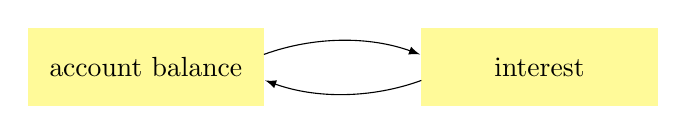
\begin{tikzpicture}
    \fill[color=yellow!40!white] (-4,2) rectangle (-1,3) node[pos=.5] {\color{black}account balance};
%    \draw (-1,2.5) -- (1,2.5);
    \fill[color=yellow!40!white] (1,2) rectangle (4,3) node[pos=.5] {\color{black}interest};
    \draw[-{latex}] (-1,2.66) arc (110:70:2.9);
    \draw[-{latex}] (1,2.33) arc (290:250:2.9);
\end{tikzpicture}	
\end{center}


\paragraph{Step 3.} Let us make the following assumptions:
\begin{itemize}
	\item We make one initial deposit into the account at time $n=0$.
	\item We don't make any more withdrawals or deposits.
	\item The only way the savings account balance changes is through the interest, which is the interest rate $p\%$ of the current balance.
\end{itemize}

\paragraph{Step 4.} We create the following model
$$ 
\begin{array}{ccccccl}
b_{n+1} & = & \big(\substack{\rm previous\\ \rm balance}\big) & + & {\rm interest} \\
b_{n+1}& =& b_n & + & \alpha \frac{p}{100} b_n & = & \left( 1 + \alpha \frac{p}{100}\right) b_n.
\end{array}
$$
	
\end{example}


\hfill

\newpage 
\submodule{Probability Models}

There are several circumstances that involve probabilities that can be modelled using difference equations.

Below is an example of one such circumstance.


\begin{example}

A gambler plays a game at a casino. The game is played one round at a time. 
\vfill

Each round, one of two things happens:
\begin{itemize}
\item The gambler wins \$1 with a probability of $q$
\item The gambler loses \$1 with a probability of $1-q$\\
\end{itemize}

The gambler will stop playing only if
\begin{itemize}
\item The gambler is ruined (bankrupt)
\item The gambler reaches $\$W$.\\
\end{itemize}

What is the probability $\pmb{p_n}$ that the player will be ruined if he starts gambling with $\$n$  ?	 \\


\paragraph{Step 2.} Mind map.
\begin{center}
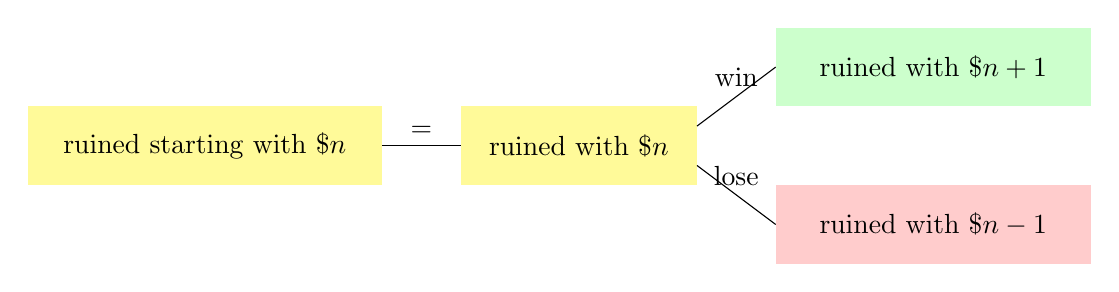
\begin{tikzpicture}
    \fill[color=yellow!40!white] (-4.5,2) rectangle (0,3) node[pos=.5] {\color{black}ruined starting with $\$n$};
    \draw (0,2.5) -- (1,2.5) node[pos=.5,above] {$=$};
    \fill[color=yellow!40!white] (1,2) rectangle (4,3) node[pos=.5] {\color{black}ruined with $\$n$};
    \draw (4,2.75) -- (5,3.5) node[pos=.5,above] {win};
    \fill[color=green!20!white] (5,3) rectangle (9,4) node[pos=.5] {\color{black}ruined with $\$n+1$};
    \draw (4,2.25) -- (5,1.5) node[pos=.5,above] {lose};
    \fill[color=red!20!white] (5,1) rectangle (9,2) node[pos=.5] {\color{black}ruined with $\$n-1$};
\end{tikzpicture}	
\end{center}


The two boxes on the left are very important. The crucial idea is to realize that it doesn't matter when the gambler has $\$n$. If s/he has $\$n$ at two different points in time, then the probability of becoming ruined is the same. \\

This mind map, shows us that we can relate $p_n$, $p_{n+1}$ and $p_{n-1}$.\\

The rest of the modelling will be left as a practice problem.

\end{example}


\begin{video}
\begin{itemize}
	\item \qrvideo{https://youtu.be/Rr2iSKlengg}
\end{itemize}	
\end{video}


\hfill


\submodule{Population Models}

We have modelled populations using differential equations. Populations can be modelled using both differential or difference equations. Which kind of equations to use depends on the goal of the model and the assumptions that we make. 

Below we'll see an example of a population model using difference equations.


\begin{example}

Model a population of mosquitoes, who reproduce at specific times of the year.

\paragraph{Step 1.} The goal is to model the population, so we define
\begin{itemize}
	\item $p(t) = $ population of mosquitoes at time $t$.
\end{itemize}



\paragraph{Step 2.} We create a mind map for this problem.

\begin{center}
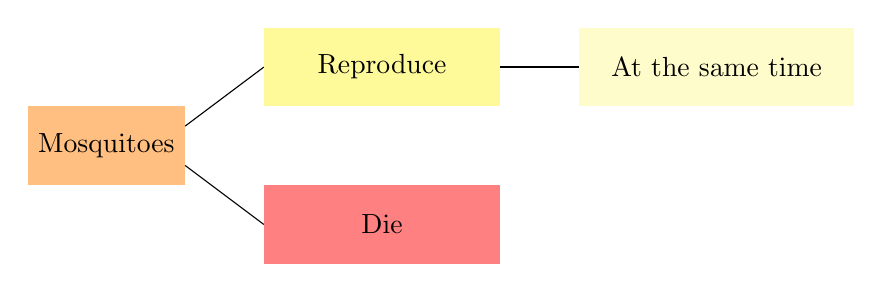
\begin{tikzpicture}
    \fill[color=orange!50!white] (-4.5,2) rectangle (-2.5,3) node[pos=.5] {\color{black}Mosquitoes};
    \draw (-2.5,2.75) -- (-1.5,3.5);
    \fill[color=yellow!40!white] (-1.5,3) rectangle (1.5,4) node[pos=.5] {\color{black}Reproduce};
    \draw (-2.5,2.25) -- (-1.5,1.5);
    \fill[color=red!50!white] (-1.5,1) rectangle (1.5,2) node[pos=.5] {\color{black}Die};
    \draw (1.5,3.5) -- (2.5,3.5);
    \fill[color=yellow!20!white] (2.5,3) rectangle (6,4) node[pos=.5] {\color{black}At the same time};
\end{tikzpicture}
\end{center}



\paragraph{Step 3.} Given that the mosquito population all reproduces at the same time, we don't need to track the population at all times $t$.

So we can assume that the mosquito population doesn't change (much) between seasons, and we change our objective function from $p(t)$ to $p_n$:
\begin{itemize}
	\item $p_n = $ population of mosquitoes at the beginning of season $n$.
\end{itemize}

We understand that mosquitoes die in between seasons, but in this model, we only count the deaths at the beginning of each season. \\

The next assumption is that the number of nymphs (baby mosquitoes) is proportional to the number of mosquitoes in the beginning of the season.

Similarly, the number of deaths is proportional to the number of mosquitoes in the beginning of the season. Also observe that mosquitoes only live for one season, which means that the proportionality constant $\mu > 1$.



\paragraph{Step 4.} So our model is
\begin{itemize}
	\item $p_n = $ population of mosquitoes at the beginning of season $n$.
	\item $p_{n+1} = r p_n - \mu p_n = (r-\mu)p_n$;
	\item $r = $ the average number of nymphs per per mosquito per season;
	\item $\mu = $ the average number of deaths per mosquito per season;
	\item $\mu > 1$, which means that each mosquito itself dies (at the end of the seasons if not earlier), but also some of its nymphs will die.
\end{itemize}

\end{example}

\begin{video}
\begin{itemize}
	\item \qrvideo{https://youtu.be/qmm9GPhA1MY}
	\item \qrvideo{https://youtu.be/j__Kredt7vY}
\end{itemize}	
\end{video}


	\newpage

\begin{exercises}

	Create a model for the following situations.
	\begin{problist}
	\prob You just took a loan to buy a car. You'll need to make fixed payments every period, and the bank will charge an interest on the amount you still owe every period.

		\begin{center}
			\includegraphics*[width=150pt]{images/module25-chirping-echo.pdf}
		\end{center}

	\prob A bird is chirping to find a mate. Unfortunately it is standing next to a cave which echoes its chirps. Consider the following:

 
			\begin{enumerate}[label={(P$_{\arabic*}$) } ]
			\item The bird chirps once every minute;
			\item The maximum volume the bird can chirp is $M$ dB;
			\item If it hears a chirp, then it chirps at a volume proportional to the volume of the chirp it heard times the difference between the maximum volume it is capable and the volume heard with constant $A \ \frac{1}{dB}$;
			\end{enumerate}



	\prob IBM just developed an new software that they wish to charge for usage. In this program, there is a parameter $n$ that you can choose to change how it performs:
			\begin{itemize}
			\item $n^2 = $ number of operations it takes to run the program;
	%		\item Each operation takes $10^{-3}$ seconds;
	%		\item The error of the result is inversely proportional to $n$, i.e., proportional to $\frac1n$;
			\item The profit IBM will make is $- \ln({\rm error})$ in Canadian dollars (negative means that IBM has to pay a penalty).
			\end{itemize}
	
			Model the profit that IBM makes. Remember to consider all sources of costs.
	
	\prob Let us study Engineering students at the University of Toronto. Find a model for the number of undergraduate students in the Engineering school at the University of Toronto and how they change from year to year. 

	\prob You are working for Canada Revenue Agency and the queue in the IRS complaints section is getting too large and lengthy. One way to solve this would be to stop collecting taxes, but that's not possible, so you are tasked with modelling the queue. 

			Model a queue on a typical weekday afternoon minute by minute. 
%			Here are some details about the queue:
%			\begin{itemize}
%			\item The average number of people joining the queue per minute is $\beta$.
%			\item On average, $\gamma\%$ of people in the queue are attended and leave the queue per minute.
%			\item Also on average $\mu\%$ of people in the queue give up waiting and leave the queue per minute.
%			\end{itemize}


	
	\prob Read the example above about the gambler's ruin. Finish creating a model for it.

	\prob A ball bouncing on the floor.
	
	\prob A person has some fever and takes tylenol every 4 hours. What is the concentration of tylenol in her bloodstream?
	
	\end{problist}
\end{exercises}

\end{module}



\begin{lesson}
	\Title{Modelling with Difference Equations}

	\Heading{Objectives}
	\begin{itemize}
		\item Bla
	\end{itemize}
	
	\Heading{Motivation} 

\end{lesson}



\begin{annotation}
\begin{goals}
	The effective annual interest rate is the interest rate with a compounding period of 1 year that gives the same result s the rate of $p\%$ compounded every $\alpha$ years.
\end{goals}
\end{annotation}
\question
	Let us expand on the economic example above.
	
	We put a certain amount of money in a savings bank account with an annual interest rate of $p\%$, and compounded at regular periods of $\alpha$ (in years). \\
	
	Even though we call $p\%$ the annual interest rate, because it is compounded during the year, at the end of the year the effective annual interest rate $p_{\rm eff}\%$ is actually higher.
	
	Calculate the effective interest rate $p_{\rm eff}\%$.


	

\bookonlynewpage


\question The goal of this quesiton is to try to understand the meaning of average lifespan.
\begin{annotation}
\begin{goals}
	\Goal{Pre-class question}
	The goal of this question is to prepare for calculating the average lifespan in the next page. \\

	Not to do in lecture. Assign to students to solve at home before.
\end{goals}
\end{annotation}
\begin{parts}
	\item Consider a small tribe, where the people in there died at the ages:		
		\begin{graybox}
		\begin{center}
			42, 56, 46, 52, 5, 103, 47, 67, 67, 85, 57, 42, 47, 67, 46, 42, 5, 46, 57, 42.
		\end{center}
		\end{graybox}
		What is the average lifespan of this tribe's population? %51.05

	\item  Consider another small tribe, where people recorded their lifespans differently. Below is a table with the percentage of the population that died at each age:
		\begin{graybox}
		\begin{center}
		\begin{tabular}{c||c|c|c|c|c|c|c}
			\textbf{Percentage of population}
				& 2\% & 5\% & 9\% & 9\% & 16\% & 22\% & 37\% \\ \hline
			\textbf{Age at death}
				& 98 & 82 & 71 & 66 & 61 & 53 & 48\\
		\end{tabular}
		\end{center}
		\end{graybox}
		What is the average lifespan of this tribe's population? %57.57
\end{parts}
 

\vfill



\bookonlynewpage



\begin{annotation}
\begin{goals}
	Some hints:
	\begin{itemize}
		\item individual dying during season $k$ $\Leftrightarrow$ lifespan $= k$ seasons
		\item From previous two exercises, deduce that: average lifespan $=$ expected value of lifespan $\ell = E$:
		$$ E = \sum_{k=0}^\infty k \ell(k) $$
		\item $\displaystyle \sum_{k=1}^\infty k r^k = \frac{r}{(1-r)^2}$ for $|r|<1$.
		\item End result should be $\frac1\mu$.
\end{itemize}	
\end{goals}
\end{annotation}
\question
	Given a population with
	\begin{itemize}
		\item $\mu=$ probability that an individual will die between two seasons.
	\end{itemize}
\begin{parts}
	\item Define the following quantity
	\begin{itemize}
		\item $P(k)=$probability that an individual born at season $0$ is alive at the beginning of season $k$.
	\end{itemize}
	Find a model for $P(k)$.

	\item What is the probability of the individual dying during the k$^{\rm th}$ season?
	\item What is the average lifespan of an individual in this population?
\end{parts}




\bookonlynewpage


\question
	Consider a population of special rabbits. Once a pair of rabbits is born, they grow and one year later they are still immature. But two years after they are born they give birth to another pair of rabbits.
	
\begin{annotation}
	\begin{goals}
		If there is time, students should show that the Fibonacci sequence does indeed match the number of rabbits.
	\end{goals}
\end{annotation}
	Model this population of rabbits.	

	


\bookonlynewpage


\question
	Consider another population of rabbits. This is the lifecycle of a pair of rabbits:
	\begin{enumerate}[start=0,label=(year \arabic*)]
		\item Born
		\item Immature (no babies)
		\item Young Adult (1 pairs of babies)
		\item Adult (1 pair of babies)
		\item Old (no babies)
		\item Die
	\end{enumerate}	
\begin{annotation}
	\begin{goals}
		Students might try to find a pattern. 
		
		It is possible, but very difficult.
		
		Hint: Use a system of difference equations. \\
		
		In core exercise \ref{rabbitscomplicatedproof}, the students are asked to prove the formula.
	\end{goals}
\end{annotation}
	
	Model this population of rabbits.
	
	




\standardonlynewpage
%
%
%
%%%%%%%%%%%%%%%%%%%%%%%%%%%%%%%
%%
%%  MODULE - Models with probabilities
%%
%%%%%%%%%%%%%%%%%%%%%%%%%%%%%%%
%
%
%
%\begin{module}{Models with probabilities}
%	\label{diff:prob}
%
%	\input{modules/module23-diff-prob.tex}
%	\input{modules/module23-diff-prob-exercises.tex}
%\end{module}
%
%
%
%\begin{lesson}
%	\Title{Models with probabilities}
%
%	\Heading{Objectives}
%	\begin{itemize}
%		\item Bla
%	\end{itemize}
%	
%	\Heading{Motivation} 
%
%\end{lesson}
%
%
%\newpage
%
%\question
%	Core Exercise with several parts
%\begin{parts}
%	\item Part 1
%	\item Part 2
%\end{parts}
%
%\bookonlynewpage
%
%
%\question
%	One more core exercise
%
%




%
%%%%%%%%%%%%%%%%%%%%%%%%%%%%%%%
%%
%%  MODULE - Models for Two or More Interconnected Quantities
%%
%%%%%%%%%%%%%%%%%%%%%%%%%%%%%%%
%
%
%
%\begin{module}{Models for Two or More Interconnected Quantities}
%	\label{diff:sys}
%
%	\input{modules/module26-diff-sys.tex}
%	\input{modules/module26-diff-sys-exercises.tex}
%\end{module}
%
%
%
%\begin{lesson}
%	\Title{Models for Two or More Interconnected Quantities}
%
%	\Heading{Objectives}
%	\begin{itemize}
%		\item Bla
%	\end{itemize}
%	
%	\Heading{Motivation} 
%
%\end{lesson}
%
%
%\newpage
%
%\question
%	Core Exercise with several parts
%\begin{parts}
%	\item Part 1
%	\item Part 2
%\end{parts}
%
%\bookonlynewpage
%
%
%\question
%	One more core exercise
%
%

%%%%%%%%%%%%%%%%%%%%%%%%%%%%%%
%
%  MODULE - Analysis of Difference Equations
%
%%%%%%%%%%%%%%%%%%%%%%%%%%%%%%



\begin{module}{Analysis of Difference Equations}
	\label{diff:analysis}

	In this module you will learn
\begin{itemize}
	\item some ways to analyze models with difference equations
\end{itemize}

\hfill \\




We have seen some different types of models involving difference equations. we have also seen a few different ways to solve them.

We will now see an example of how we can analyze a difference equation.



\begin{example}

Consider the following model for the number of Mathematics students at a University:
\begin{itemize}
\item $e_k = $ number of students in the year $2020+k$;
\item $a_k = $ number of students admitted to the first year;
\item $g = $ percentage of students that graduate every year;
\item $q = $ percentage of students that quit the Mathematics program  every year. \\

\item $e_{k+1} = e_k + a - g e_k - q e_k$
\end{itemize}

\end{example}

\hfill

\begin{center}
\textbf{\color{cyan}
Finding the equilibrium point(s)
}
\end{center}


What is the equilibrium number of students $E$? This means that we are looking for a solution that remains constant $e_{k+1}=e_k = E$.

$$
E = E + a - (g+q)E
\quad \Leftrightarrow\quad
	E = \frac{a}{g+q}
$$

This is the value that the department should strive for, since it would remain stable.


%\newpage
\hfill

\begin{center}
\textbf{\color{cyan}
Numerical approximations
}
\end{center}


For models with difference equations, we don't need numerical methods, since the recursive definition of the sequence is already a numerical method in itself.

We can follow the same approach however and run some numbers and with different values for the parameters to gain some intuition on the solutions.

\begin{center}
\begin{tabular}{cc}
\includegraphics*[width=150pt]{images/module26-stud-above.png}
	& \includegraphics*[width=150pt]{images/module26-stud-below.png} \\
$e_0 > E$ 
	& $e_0 < E$
\end{tabular}
\end{center}
 

\begin{graybox}
You can access this simulation here:
\begin{itemize}
	\item \qrvideo{https://www.desmos.com/calculator/wv3oxrjvrz}
\end{itemize}	
\end{graybox}


\hfill

\begin{center}
\textbf{\color{cyan}
Qualitative evolution of quantities
}
\end{center}


Let us now look at what happens if the situation is not in equilibrium. The numerical study above, gives some intuition about the behaviour of solutions. 

Let us assume that $e_k  > E$. Then
\begin{align*}
e_{k+1}
	& = e_k (1-g-q) + a \\
	& > E (1-g-q) + a \tag{see note below} \\
	& = E - E(g+q)+a \\
	& = E - \frac{a}{g+q}(g+q) + a\\
	& = E
\end{align*}

\begin{graybox}
\textbf{Note. } This step is only true if $E$ and $1-g-q>0$. (Why?) \\

It's clear that $E$ should be positive, since it is a number of students. \\

The other quantity is not so obvious: \quad $g+q < 1$ ?

In fact, $g+q$ is the fraction of students that graduate or quit the Mathematics program, so it can't exceed 1! (Why?)
\end{graybox}


We conclude that if $e_k > E$, then $e_{k+1}>E$. This means that if the number of students starts above the equilibrium, then it will always stay above it.\\

But will the number of students keep increasing without bound or will it converge to a number?\\

Let us check:
\begin{align*}
e_{k+1} - e_k
	& = a - e_k (g+q) \\
	& < a - E (g+q) \\
	& = a - \frac{a}{g+q} (g+q) \\
	& = 0
\end{align*}

So we conclude that 
$$
e_{k+1} - e_k < 0 \quad \Leftrightarrow \quad e_{k+1} < e_k,
$$
so the number of students will decrease.

Our conclusion is that if $e_k > E$, then $e_{k+1} \in [E, e_k]$:
\begin{center}
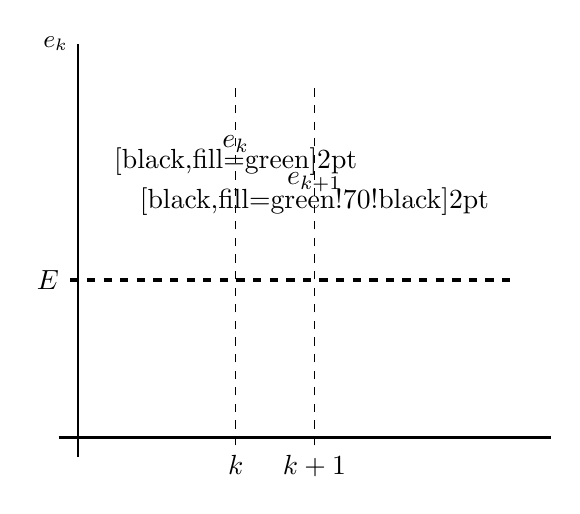
\begin{tikzpicture}
  \draw[thick,-{\seta}] (-0.25,0) -- (6,0) ;%node[above] {\small $k$};
  \draw[thick,-{\seta}] (0,-0.25) -- (0,5) node[left] {\small $e_k$};
%  \draw[] (2,0) node[below] {$k$};
  \draw[dashed] (2,-0.1) node[below] {$k$} -- (2,4.5);
%  \draw[] (3,0) node[below] {$k+1$};
  \draw[dashed] (3,-0.1) node[below] {$k+1$} -- (3,4.5);
  \draw[ultra thick,dashed] (-0.1,2) node[left] {$E$} -- (5.5,2)  ;
%
  \draw (2,3.5) node {\tikzcircle[black,fill=green]{2pt}} node[above] {$e_{k}$};
  \draw (3,3) node {\tikzcircle[black,fill=green!70!black]{2pt}} node[above] {$e_{k+1}$};
\end{tikzpicture}
\end{center}


Similarly, if $e_k < E$, we can conclude that $e_{k+1} \in [e_k,E]$:
\begin{center}
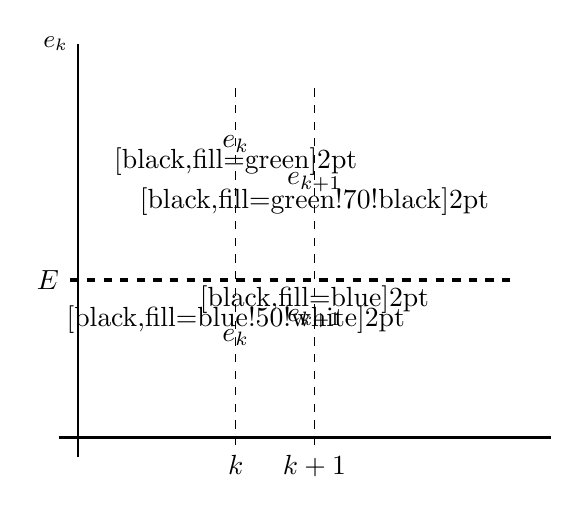
\begin{tikzpicture}
  \draw[thick,-{\seta}] (-0.25,0) -- (6,0) ;%node[above] {\small $k$};
  \draw[thick,-{\seta}] (0,-0.25) -- (0,5) node[left] {\small $e_k$};
%  \draw[] (2,0) node[below] {$k$};
  \draw[dashed] (2,-0.1) node[below] {$k$} -- (2,4.5);
%  \draw[] (3,0) node[below] {$k+1$};
  \draw[dashed] (3,-0.1) node[below] {$k+1$} -- (3,4.5);
  \draw[ultra thick,dashed] (-0.1,2) node[left] {$E$} -- (5.5,2)  ;
%
  \draw (2,3.5) node {\tikzcircle[black,fill=green]{2pt}} node[above] {$e_{k}$};
  \draw (3,3) node {\tikzcircle[black,fill=green!70!black]{2pt}} node[above] {$e_{k+1}$};
  \draw (2,1.5) node {\tikzcircle[black,fill=blue!50!white]{2pt}} node[below] {$e_{k}$};
  \draw (3,1.75) node {\tikzcircle[black,fill=blue]{2pt}} node[below] {$e_{k+1}$};
\end{tikzpicture}
\end{center}


So we can see that the sequence $e_k$ will be approaching $E$, so we can say that the \emph{equilibrium is stable}.







\hfill

\begin{center}
\textbf{\color{cyan}
Limiting behaviour of the solutions
}
\end{center}



From our previous analysis, we can see that it looks like 
$$
\lim_{k \to \infty} e_k = E.
$$

But we didn't prove this yet. It could be that the sequence converges to some other value. 

To show this, we would need to define a new sequence $x_k = e_k-E$, assume that it has the form $x_k = C r^k$ and then obtain a characteristic equation for $r$:
$$
r = 1-g-q \in (0,1),
$$
so $x_k = C r^k$ and 
$$
\lim_{k \to \infty} x_k = 0
\quad \Leftrightarrow \quad
	\lim_{k \to \infty} e_k = E.
$$

So we now know that the number of students will converge monotonically to the equilibrium.








	\newpage 

\begin{exercises}

		\begin{problist}
	
	\prob Consider the following discrete population model:
	\begin{itemize}
		\item $p_k=$ population at the beginning of season $k$
		\item $R = $ basic reproduction value for the population
		\item $K= $ carrying capacity 
		\item $\displaystyle p_{k+1}=p_k + R p_k\left(1-\frac{p_k}{K}\right)$
	\end{itemize}
	
	\begin{enumerate}
		\item Define:
		\begin{itemize}
			\item $\mu = 1+R$,
			\item $\displaystyle x_k = \frac{R}{1+R} \frac{p_k}{K}$.
		\end{itemize}
		Show that $x_{k+1} = \mu x_k (1-x_k)$.
		\item What are the equilibrium values for $x_k$?
	%	$$
	%	E = 1 - \frac1\mu = \frac{mu-1}{\mu}
	%	$$
	
		\item Take $R=1, \mu=2$. Compare this model with the continuous logistic model.
		\item In the continuous model, solutions cannot cross the equilibrium. 
		Change the value of $R,\mu$ and show that in this discrete model, solutions can cross the equilibrium.
		
		\item Take $R=3, \mu=4$ (constants for influenza virus). Below is a graph with $\color{green!70!black}x_0 = 0.1$ and $\color{blue!85!black}x_0=0.101$.
	
			\begin{center}
				\includegraphics*[width=150pt]{images/module26-logistic.png}
			\end{center}
		
			Which conclusions do you take from this graph?
			
		\item Take $x_0=\frac12$. What happens to $x_k$ as $k$ gets larger and larger: does it remain bounded, or does it converge to $\pm \infty$? Check for different values of $\mu$.

		\item You'll need to program for this exercise. Now allow complex values for $\mu \in \mathbb{C}$. In a graph, mark the values of $\mu \in \C$, for which $x_n$ does not diverge to infinity.
		
%		\includegraphics*[width=150pt]{images/module26-mandelbrot.png}
		
	\end{enumerate}

\begin{annotation}
\begin{goals}
	\begin{itemize}
	\item[1.] You can skip the first part and tell students to do it at home.
	
	\item[3.] For the comparison part, notice how the model is very similar in the way it looks. If you run the model it also behaves very similarly.

	\qrvideo{https://www.desmos.com/calculator/zxk8udxmac}
	
	\item[4.] For the last part, for $\mu=3$, solutions oscillate but converge to equilibrium
	\item[5.] For the last part, for $\mu=4$, $x_0=0.1$ and $x_0=0.101$ gives completely different solutions. Chaotic behaviour. So need to be careful analyzing nonlinear difference equations.
	
		\qrvideo{https://www.desmos.com/calculator/e656u8n4vt}
	\end{itemize}
\end{goals}	
\end{annotation}

	

	

	\prob Consider the model for a queue:
	\begin{itemize}
		\item $q_n=$ number of people waiting in the queue at minute $n$;
		\item $\gamma=$ fraction of the people waiting that are attended each minute;
		\item $\mu=$ average number of people that give up waiting in the queue per minute;
	\end{itemize}

	\begin{enumerate}
		\item First, let us find out a very bad scenario for the queue. Find a number of initial people in the queue $q_0$ such that the size of the queue will never change.
		\item Let 
			\begin{itemize}
				\item $p_k=$ probability that a person who joined the queue at time $k=0$ will still be waiting after $k$ minutes.
			\end{itemize}
			Is $p_k$ increasing, decreasing, or not monotone?
		\item The probability that someone waited exactly $k$ minutes is $p_{k}-p_{k+1}$.
			Find another expression for $p_{k}-p_{k+1}$ without using $p_k$.
		\item The expected waiting time in the queue is given by the ``law'':
			
			\hspace{-.05\textwidth}\framebox{
			\begin{minipage}{.4\textwidth}
			The expected waiting time is the weighted average of the possible waiting times, where the weights are the probability of waiting that exact amount of time.
			\end{minipage}}
			
		Find the expected waiting time for this queue.
	\end{enumerate}
	
	
	
	
	
	\prob 	Two computers are facing each other on video conferencing software. The first computer makes a sound and every fraction of a second, the other computer reproduces the sound.
	
	Consider the following model for the microphone feedback:
	\begin{itemize}
		\item $v_n =$ volume produced by the first computer (in dB) for the $n$ iteration;
		\item $e=$ fraction of the original volume reproduced by the second computer;
		\item $M=$ maximum volume that first computer can produce (in DB). \\

		\item $v_{n+1} = e v_n \left( \frac{M - e v_n}{M}+1\right)$.
	\end{itemize}
	
	\begin{enumerate}
		\item What is the initial volume that will just cause the following iterations to be the same?


		\item Find a condition on $e$ that allows for the previous situation to occur.

%v>0 iff 
%v<M iff 

		\item Assume $e \in (0,1)$. What happens if the initial volume is softer than the equilibrium? What happens if the initial volume is louder than the equilibrium?
		\item Assume $e>1$. What happens if the initial volume is softer than the equilibrium? What happens if the initial volume is louder than the equilibrium?

		\item Assume $e=\frac85$. Sketch a graph of the solution.
		
%		\begin{itemize}
%			\item $v_0 = M$	
%			\item $v_1 = \frac{16}{25}M$
%			\item $v_2 = \frac85 \frac{16}{25}M \frac{122}{125} \approx M$
%		\end{itemize}

		What is the behaviour of the solution as $n$ gets larger?
		
		\item Assume $e=\frac{1+\sqrt{5}}{2}$ the golden ratio. Is there an initial volume that gives a periodic solution: $v_0=v_2=v_4,v_5=\cdots$ and $v_1=v_3=v_5=v_7=\cdots$?
	
	\end{enumerate}
	
\begin{annotation}
\begin{goals}
	For 2, remember that the first computer has to be able to produce the sound: $v_n < M$, and the sound needs to be audible $v_n>0$.
\end{goals}	
\end{annotation}


		
	\end{problist}
\end{exercises}
\end{module}



\begin{lesson}
	\Title{Analysis of Difference Equations}

	\Heading{Objectives}
	\begin{itemize}
		\item Bla
	\end{itemize}
	
	\Heading{Motivation} 

\end{lesson}




\question 
	Consider the following difference equation:
		$$u_{k+1} = a(u_k - b)$$

	\begin{parts}
		\item What is the equilibrium solution?
		\item Are there 2-periodic solutions? I.e. satisfying
\begin{annotation}
	\begin{goals}
		\begin{itemize}
			\item In the calculations for .2, there is a step that involves a division by $(1-a^2)$, so it can only be done for $a \neq \pm 1$.
			\item The final result for .2 is:
			\begin{align*}
				a \neq \pm1. & \quad {\rm periodic} \Rightarrow u_0 = \frac{ab}{a-1} \quad & \Rightarrow & 1-{\rm periodic} \\
				a = 1. & \quad {\rm periodic} \Rightarrow b=0  & \Rightarrow & 1-{\rm periodic} \\
				a = -1. & \quad {\rm periodic} \Rightarrow b=0  & \Rightarrow & 2-\text{periodic if } u_0\neq 0
			\end{align*}
		\end{itemize}
	\end{goals}
\end{annotation}
		\begin{itemize}
			\item $v_0=v_2=v_4=v_6=\cdots$
			\item $v_1=v_3=v_5=v_7=\cdots$
			\item $v_0\neq v_1$
		\end{itemize} 
		\item What happens to the solutions for different values of $a$?
		\item What happens to the solutions for different values of $b$?
	\end{parts}






\bookonlynewpage

\question
	Consider a drunkard that is walking randomly near a cliff.

	\hfill \includegraphics*[width=250pt]{images/module26-drunk.pdf}
	\vspace{-70pt}

	\begin{minipage}{.9\textwidth}
		Consider this model for the drunkard's chance of getting to safety from falling off the cliff:
		\begin{itemize}
			\item $q$ is the probability that the drunkard will step towards safety;
			\item $1-q$ is the probability that the drunkard will step towards the cliff;
			\item $p_n=$ probability that the drunkard will get to safety if he is in step number $n$; 
			\item The drunkard will stop moving if he gets to safety (step $W$) or if he falls out of the cliff (step $0$); \\
	
			\item $p_n = q p_{n+1} + (1-q) p_{n-1}$. \\
		\end{itemize}
	\end{minipage}

	
\begin{annotation}
	\begin{goals}
		Question .3 is purposefully ambiguous about symmetry. What kind of symmetry is there? Is there any?
	\end{goals}
\end{annotation}
	\begin{parts}
		\item Is $p_n$ increasing or decreasing?
		\item What is $p_0$? What is $p_W$?
		\item Let $q=\frac12$. What is $p_{W/2}$? Is $p_n$ symmetric around $n=\frac{w}{2}$?
		\item Let $q>\frac12$. Is $p_{W/2} > \frac12$? Is $p_{W/2} < \frac12$? 
		\item How do solutions for $q=\alpha$ and $q=1-\alpha$ compare?
	\end{parts}


	
\bookonlynewpage

\hfill

\bookonlynewpage


\begin{minipage}{.45\textwidth}
\question \label{rabbitscomplicatedproof}
	Consider a population of rabbits with the following lifecycle:
	\begin{enumerate}[start=0,label=(year \arabic*)]
		\item Born
		\item Immature (no babies)
		\item Young Adult (1 pair of babies)
		\item Adult (1 pair of babies)
		\item Old (no babies)
		\item Die \\[5pt]
	\end{enumerate}	
	
\end{minipage}
\qquad
\begin{minipage}{.45\textwidth}
	Consider the definitions:
	\begin{itemize}
		\item We start with 1 pair of newborn rabbits in year 0;
		\item $r_n=$ number of pairs of rabbits alive during year $n$;
		\item $i_k=$ number of immature pairs;
		\item $y_k=$ number of young adult pairs;
		\item $a_k=$ number of adult pairs;
		\item $o_k=$ number of old pairs.
	\end{itemize}

\end{minipage}

	\begin{parts}
		\item Show that $b_k=b_{k-2}+b_{k-3}$.
		\item Show that $y_{k+1}=o_{k}+o_{k+1}$.
		\item Show that $r_{n} = r_{n-2}+r_{n-3}$.
	\end{parts}

\begin{annotation}
\begin{goals}
$$
r_k 
	= {\color{magenta}r_{k-1}-o_{k-1}}+{\color{blue}b_k}
$$

On the other hand, 
$$
\color{magenta}
r_{k-1}-o_{k-1}
  = b_{k-2} + 2 y_{k-2} + a_{k-2} 
  = r_{k-2} + y_{k-2} - o_{k-2}
$$
and
$$
\color{blue}
b_k 
  = b_{k-2}+b_{k-3}
  = y_{k-3} + a_{k-3} + b_{k-3}
  = r_{k-3} - o_{k-3}
$$

So we have
$$
r_k = {\color{magenta}r_{k-2} + {\color{black}\not} y_{k-2} - {\color{black}\not} o_{k-2}} + {\color{blue}r_{k-3} - {\color{black}\not}o_{k-3}}
= r_{k-2} + r_{k-3}
$$
\end{goals}
\end{annotation}	

	
	

\standardonlynewpage

%
%
%%%%%%%%%%%%%%%%%%%%%%%%%%%%%%%
%%
%%  MODULE - Nonlinear Models
%%
%%%%%%%%%%%%%%%%%%%%%%%%%%%%%%%
%
%
%
%\begin{module}{Nonlinear Models}
%	\label{diff:nonlinear}
%
%	In this module you will learn
\begin{itemize}
	\item some nonlinear models
	\item some of the difficulties of studying nonlinear models
\end{itemize}

\hfill \\


%	\begin{exercises}

	\begin{problist}
	\prob Show that all autonomous differential equations are separable.

	\end{problist}
\end{exercises}

%\end{module}
%
%
%
%\begin{lesson}
%	\Title{Nonlinear Models}
%
%	\Heading{Objectives}
%	\begin{itemize}
%		\item Bla
%	\end{itemize}
%	
%	\Heading{Motivation} 
%
%\end{lesson}
%
%
%\newpage
%
%\question
%	Core Exercise with several parts
%\begin{parts}
%	\item Part 1
%	\item Part 2
%\end{parts}
%
%\bookonlynewpage
%
%
%\question
%	One more core exercise
%
%











%%%%%%%%%%%%%%%%%%%%%%%%%%%%%%%%%%%%%%%%%%%%%%%%%%%%%%%%%%%%%%%%%%%%%%%%
%
%		Chapter 6 - Projects
%
%%%%%%%%%%%%%%%%%%%%%%%%%%%%%%%%%%%%%%%%%%%%%%%%%%%%%%%%%%%%%%%%%%%%%%%%


\begin{bookonly}
	
%%%%%%%%%%%%%%%%%%%%%%%%%%%%%%%%%%%%%%%%%%%%%%%%%%%%%%%%%%%%%%%%%%%%%%%%
%
%		Chapter 6 - Projects
%
%%%%%%%%%%%%%%%%%%%%%%%%%%%%%%%%%%%%%%%%%%%%%%%%%%%%%%%%%%%%%%%%%%%%%%%%


\begin{topic}[Projects]


\vfil

\begin{center}
\begin{minipage}{450pt}
	\includegraphics*[width=450pt]{images/chap6-xkcd.png}

	\hfill {\footnotesize (image from \href{https://www.xkcd.com/557/}{xkcd - comic \#557})}
\end{minipage}
\end{center}
\end{topic}








			%%%%%%%%%%%%%%%%%%%%%%%%%%%%%
			%							%
			%  FIRST-ORDER ODE			%
			%							%
			%%%%%%%%%%%%%%%%%%%%%%%%%%%%%



%%%%%%%%%%%%%%%%%%%%%%%%%%%%%%
%
%  Project - Managing a Fishery
%
%%%%%%%%%%%%%%%%%%%%%%%%%%%%%%



\begin{project}{Managing a fishery}
	\label{proj:fishery}

	The population $P(t)$ of a species of fish in a finite environment, like a lake is often described by the logistic equation
$$
\frac{dP}{dt} = r P \left(1 - \frac{P}{K} \right),
$$
where $r$ is the natural growth rate of the population and $K$ is the maximum number of individuals that the environment can sustain. \\

If that population is harvested at the rate of $H(t,P)$ fish per year, then it can be modelled by the ODE
\begin{emphbox}[]
$$
\frac{dP}{dt} = r P \left(1 - \frac{P}{K} \right) - H(P,t).
$$
\end{emphbox}


This ODE assumes that the population is harvested continuously throughout the year, which is not exactly true. Later in the course we will see how to make a better model. \\


Your goal is to figure out the maximum profit you can generate from this population of fish. For that, it should be clear that it is undesirable to harvest too much, since it may lead to the extinction of the fish.


\emph{1. Selling fishing licenses.}
As the manager of the lake, you decide to profit from it by selling fishing licenses to people and allow them to fish there. 

\begin{enumerate}[label=\emph{(\alph*)}]
\item Assuming that an average person, after a whole \emph{day} fishing, has an efficiency\footnote{Efficiency of $E\%$ means that after a whole day fishing, that person will have caught $E\%$ of the existing fish in the lake.} of $E\%$, what is $H(P,t)$ and what is the ODE that models the fish in the lake?

\item There is a percentage $E^\star$, such that if $E \geq E^\star$, then the population will become extinct. What is $E^\star$? Explain why the population will become extinct.

\emph{Hint.} You don't need to solve the ODE.

%{\bf Hint for TA to give if needed. } What are the equilibrium points of the ODE? Are they stable or unstable?


\item A sustainable yield $Y$ is the rate at which the fish can be harvested indefinitely: it is the value of $H(P,t)$ which doesn't change with time and for the asymptotically stable population.

Determine the maximum\footnote{This value can be controlled, e.g. by defining the time available for fishing in a day.} value of $E$ to maximize $Y$ and then find the maximum $Y_{\max}$.

%{\bf Hint for TA to give if needed. } asymptotically stable population = stable equilibrium point

%{\bf Hint for TA to give if needed. } Find $Y$ as a function of $E$.

\end{enumerate}







\vfill

\emph{2. Selling fish.}
As the manager of the lake, you decide to profit from it by harvesting the fish yourself and selling it. 

\begin{enumerate}[label=\emph{(\alph*)}]
\item Now the fish are harvested at a constant rate $h$. What is $H(P,t)$ and what is the ODE that models the fish in the lake?

\item There is a rate $h^{\star}$, such that if $h \geq h^\star$, then the population will become extinct. What is $h^\star$? Explain why the population will become extinct.

\emph{Hint.} You don't need to solve the ODE.

%{\bf Hint for TA to give if needed. } What are the equilibrium points of the ODE? Are they stable or unstable?


\item If $h \leq h^\star$, what is the maximum sustainable yield $Y_m$?

\end{enumerate}



\vfill

\emph{Further Investigation.}
\begin{enumerate}[label=\emph{\arabic*.}]
\item Can you think of other forms for $H(P,t)$? 

\item If, instead of a logistic model, you include an extinction threshold as well, what can you say about the model for constant effort fishing? for constant rate fishing? Is it a useful addition to the model? Have fun with it!
\end{enumerate}

\begin{noexercises}
\end{noexercises}

\end{project}









%%%%%%%%%%%%%%%%%%%%%%%%%%%%%%
%
%  Project - X-Ray Attenuation
%
%%%%%%%%%%%%%%%%%%%%%%%%%%%%%%



\begin{project}{X-ray attenuation}
	\label{proj:xray}

	An X-ray tube fires X-rays, which travel in a straight line. 
An X-ray detector will give you the intensity of any X-ray that hits the detector. 
If there is a vacuum between the X-ray tube and the X-ray detector, then the X-ray will have the same intensity when it hits the detector as when it left the tube. 
However, when X-rays pass through matter they interact with the atoms in the material and are sometimes deflected off course, or absorbed. 
We call this phenomenon \emph{attenuation of the X-ray} and it results in a decrease in the intensity of the X-ray beam. 
When this happens, the X-ray detector will show a lower intensity than the original intensity of the X-ray.

The intensity of an X-ray is measured in keV (kiloelectronvolt).

\vfill

\emph{Task.}

\begin{enumerate}[label=\emph{\arabic*.}]
\item Experiments indicate that the rate of decrease in the intensity of the X-ray beam as it travels through some matter is proportional to the \emph{linear absorption coefficient} $A$ of the material. Find an ordinary differential equation (ODE) to model the intensity, $I$, of an X-ray beam fired into some uniform matter with linear absorption coefficient $A$. Be sure to include an initial condition.
\begin{itemize}
\item What are the units of $A$?
\item Classify the equation.
\item Solve the equation in terms of the initial condition and $A$. 
\end{itemize}

\vfill

\item How far into a material can an X-ray beam travel before its intensity has decreased to $\displaystyle \frac{1}{e}$ times its original intensity.
\end{enumerate}

\vfill

Now you will explore one of the main ideas behind medical X-ray imaging. In order to do this, you need to know the linear attenuation coefficient of healthy human tissue. 

\vfill

\begin{enumerate}[resume,label=\emph{\arabic*.}]
\item You have a 15keV X-ray tube and an X-ray detector. When you fire the X-ray through 10cm of healthy tissue, you measure $\displaystyle \frac{15}{e}$keV on your X-ray detector. When you fire the X-ray through 20cm of healthy tissue, you measure $\displaystyle \frac{15}{e^2}$keV. Using your model of X-ray attenuation, estimate the linear attenuation coefficient of healthy tissue.
\end{enumerate}

\vfill

This is the basis for using X-ray Computed Tomography (CT) used in medical imaging! We can recognize healthy versus unhealthy tissue by using what we know about their attenuation coefficients. To do this in a human body requires more advanced mathematics such as the Radon transform introduced in 1917 by Johann Radon. However, consider a simple case below.

\vfill

\begin{enumerate}[resume,label=\emph{\arabic*.}]
\item Suppose that you have a 10cm $\times$ 2cm rectangle with the same linear attenuation coefficient as healthy tissue, and somewhere inside this square is a circle of unknown size having a linear attenuation coefficient different from that of healthy tissue.
\begin{itemize}
\item  Using an X-ray tube and an X-ray detector, can you locate the circle and determine its radius? How?
\item  Can you determine the linear attenuation coefficient of the circle? How?
 \end{itemize}

 \vfill
 
 \item In actuality, a more complex model is needed for accurate imaging. The linear attenuation coefficient is actually dependent on the intensity of the X-ray! How does this impact your model? Discuss how this would impact your solutions to the above problems.

\end{enumerate}

\hfill ``X-Ray Attenuation'' is a collaboration between Bernardo Galv\~ao-Sousa and Craig Sinnamon.
\begin{noexercises}
\end{noexercises}
\end{project}










%%%%%%%%%%%%%%%%%%%%%%%%%%%%%%
%
%  Project - Pursuit curve
%
%%%%%%%%%%%%%%%%%%%%%%%%%%%%%%



\begin{project}{Predator-prey chase}
	\label{proj:pursuit}

	\emph{Question.} 
What is the path of a lion chasing an antelope?

\vfill

\begin{graybox}
\emph{Rules. } 
\begin{itemize}
\item The antelope flees at a constant speed $v$ in a straight line
\item The lion chases at a constant speed $u$
\end{itemize}
\end{graybox}



\vfill

\emph{Task.}
\begin{enumerate}[label=\emph{\arabic*.}]

\item Assume the antelope starts at $(0,0)$ and moves up the $y$-axis. What is its position?

$$ (0,vt) $$

\item Assume the lion's position is $\big(x(t),y(t)\big)$. What happens if $x(0)=0$?
%    
%    if $y(0)<0$, then 
%    $$y(t)=y_0+ut$$
%    otherwise
%    $$y(t) = y_0-ut$$

\item \label{sign} Assume the lion's position is $\big(x(t),y(t)\big)$ with $x(0)\neq 0$. For simplicity, assume that $x(0)<0$. What is the sign of $x'(t)$?

%    $$x'(t)>0$$

\item \label{func} The goal is to find the path, so we are looking for an equation to describe $y(x)$. Using the result from \ref{sign}, explain why the solution will be a function $y(x)$.

%    $x'(t)>0$, so the graph will be going to the right and will pass the vertical line test. This means that the path will form a graph of a function $y(x)$.

\item \label{speed} The lion's speed is $u$. Express that condition using $x(t)$ and $y(t)$.

%    $$\big(x'(t)\big)^2 + \big(y'(t)\big)^2 = u^2$$

\item Find an expression for $\dfrac{dx}{dt}$ without the variable $t$. 
%    TA hint: Use \ref{func} and \ref{speed}
%    
%    \begin{gather*}
%    \frac{dy}{dt} = \frac{dy}{dx} \frac{dx}{dt} \\
%    \left(\frac{dx}{dt}\right)^2 \left[ 1 + \left(\frac{dy}{dx}\right)^2 \right] = u^2 \\
%    \frac{dx}{dt} = \frac{u}{\sqrt{1 + \big(y'(x)\big)^2}}
%    \end{gather*}
%    

\item \label{slope} Which condition on $\dfrac{dy}{dx}$ do we get from the fact that the lion is chasing the antelope? Draw a picture.

%    $$ \frac{dy}{dx} = \frac{y - vt}{x}$$

\item Use \ref{slope}, and obtain an expression for $\dfrac{dx}{dt}$ in terms of $\dfrac{d^2y}{dx^2}$. 
%    TA hint: Recall that $\frac{dz}{dt} = \frac{dz}{dx} \frac{dx}{dt}$.
%    
%    \begin{gather*}
%    x \frac{dy}{dx} = y-vt \\
%    \frac{dx}{dt} \frac{dy}{dx} + x \frac{d^2y}{dx^2}\frac{dx}{dt} = \frac{dy}{dx}\frac{dx}{dt} - v \\
%    \frac{dx}{dt} = -\frac{v}{x \frac{d^2y}{dx^2}}
%    \end{gather*}


\item Obtain a Differential Equation that describes the lion's path $y(x)$.

%    \begin{gather*}
%    \frac{u}{\sqrt{1 + \big(y'(x)\big)^2}} = -\frac{v}{x \frac{d^2y}{dx^2}} \\
%    x y''(x) = -\frac{v}{u} \sqrt{1 + \big(y'(x)\big)^2}
%    \end{gather*}

\item For simplicity, assume that the lion starts at $(-1,0)$. Solve this Initial-Value problem. 

%    TA hint 1: $\rm arc\,sinh\,x = \ln \big(x+\sqrt{1+x^2}\big)$.
%    
%    TA hint 2: $y'(-1)=0$ because initially $x=-1$ and the lion is facing the antelope at the origin. 
%    
%    \begin{gather*}
%    z(x) = y'(x) \\
%    x z'(x) = -\frac{v}{u} \sqrt{1 + z^2} \\
%    \int \frac{1}{\sqrt{1 + z^2}} \, dz = -\frac{v}{u} \ln |x| + A \tag{$z = \sinh w$} \\
%    w = -\frac{v}{u} \ln |x| + A \\
%    {\rm arc\,sinh\,} z = -\frac{v}{u} \ln (-B x)   \tag{$x<0$} \\
%    \ln \big(z + \sqrt{1 + z^2} \big) = -\frac{v}{u} \ln (-Bx)  \tag{$k = \frac vu>0$}\\
%    z + \sqrt{1+z^2} = C (-x)^{-k} \\
%    1 + z^2 = C^2 (-x)^{-2k} + z^2 - 2 C z (-x)^{-k} \\
%    z = \frac12 \left[ C (-x)^{-k} - \frac{1}{C} (-x)^k \right] \\
%    y = \int z \, dx = \frac12 \left[ \frac{1}{C(1+k)} (-x)^{k+1} - \frac{C}{1-k} (-x)^{-k+1} \right]  + D\\
%    y(-1)=0 \text{ and } y'(-1)=0 \\
%    C = 1 \text{ and } D = \frac{k}{1-k^2} \tag{$u\neq v$}\\
%    y = \frac12 \left[ \frac{1}{1+k} (-x)^{k+1} - \frac{1}{1-k} (-x)^{-k+1} \right]  + \frac{k}{1-k^2}\\
%    \end{gather*}
%    
%    \begin{center}
%    \includegraphics*[width=250pt]{lion_antelope.pdf}
%    \end{center}

\item When does the lion actually catch the antelope?

%    \begin{gather*}
%    x=0 \\
%    y=\frac{k}{1-k^2}  = \frac{vu}{u^2- v^2} \\
%    \text{ interception for $y>0$ only if } u>v  \\
%    y = vT \tag{antelope} \\
%    T = \frac{u}{u^2- v^2}
%    \end{gather*}


\end{enumerate}









\vfill

\emph{Further investigation. } 

\begin{enumerate}[label=\emph{\arabic*.}]
\item Program the pursuit (it will be approximated) and check your answer.
\item Can you figure out the path of the lion for other antelope trajectories? 
Program that pursuit and check your answer.

\item (for fun) Program a ``game'' where you control the antelope and the computer controls the lion.
\end{enumerate}






%    WITHOUT CONSIDERING FIXED LION SPEED
%
%    \begin{gather*}
%    \frac{dx}{dt} = -x \\
%    \frac{dy}{dt} = v t - y \\
%    \\
%    \frac{dy}{dx} = - \frac{vt - y}{x}\\
%    x = -\frac{vt-y}{\frac{dy}{dx}}
%    \\
%    \frac{dx}{dt} = -\frac{(v-\frac{dy}{dt})\frac{dy}{dx} - (vt-y) \frac{d}{dt} \frac{dy}{dx}}{(\frac{dy}{dx})^2} \\
%    -x \left( \frac{dy}{dx}\right)^2	= (v-vt+y)\frac{vt - y}{x} - (vt-y) \frac{d^2y}{dx^2} x \\
%    - \frac{vt-y}{x}	= \frac{v-vt+y}{x} - \frac{d^2y}{dx^2} x \\
%    \frac{dy}{dt} = \frac vx + \frac{dy}{dt} - \frac{d^2y}{dx^2} x \\
%    \frac{d^2y}{dx^2} = \frac{v}{x^2} \\
%    \frac{dy}{dx} = -\frac vx + A \\
%    y = -v \ln |x| + Ax + B\\
%    \\
%    y(-1)=0 \text{ and } 
%    y'(-1)=0 \\
%    y'(-1)=v+A = 0 \Rarrow A=-v \\
%    y(-1) = -A+B = v+B = 0 \Rarrow B = -v \\
%    \\
%    y = -v (\ln |x| + x + 1)\\
%    %
%    %
%    \end{gather*}

\begin{noexercises}
\end{noexercises}
\end{project}




			%%%%%%%%%%%%%%%%%%%%%%%%%%%%%
			%							%
			%  SYSTEMS OF ODES			%
			%							%
			%%%%%%%%%%%%%%%%%%%%%%%%%%%%%





%%%%%%%%%%%%%%%%%%%%%%%%%%%%%%
%
%  Project - Modelling an Epidemic
%
%%%%%%%%%%%%%%%%%%%%%%%%%%%%%%



%\begin{project}{Epidemic modelling}
%	\label{proj:epidemic}
%
%	\emph{Goal.} We want to model the spread of an epidemic, like the recent Ebola epidemic in Africa.

\vfill


\emph{SIR Model.} To model an infectious disease, we divide the population in 3 groups:
\begin{itemize}
\item Susceptible Individuals $S(t) = $ number of people who haven't contracted the disease;
\item Infected individuals $I(t)= $ number of people infected;
\item Removed individuals $R(t)=$ number people that either died or recovered from the disease and are now immune to it.
\end{itemize}

\vfill

\emph{Assumptions.} 

\begin{enumerate}[label=\emph{(\alph*)}] 
\item Population size $N$ is large and constant (no birth, death, or migration)
\item No latent/incubation period
\item Homogeneous population
\item Infection rate is proportional to the proportion of infected people with constant $\beta$
\item ``Recovery'' rate is constant $\gamma$ (includes rate at which people die or recover from the disease)
\item The typical time until recovery is $T = \dfrac{1}{\gamma}$
\end{enumerate}

\vfill

\emph{ODE. } From here we can obtain the SIR model:

\begin{emphbox}[]
\begin{align*}
\frac{dS}{dt} \quad & = \quad \text{proportional to $S(t)$ and the constant is the infection rate \emph{(e)}} 
	 \quad = \quad  - \beta \underbrace{\frac{I(t)}{N}}_{\substack{\text{proportion of}\\\text{infected people}}}S(t) \\
%	\\
\frac{dI}{dt} \quad & = \quad \underbrace{\beta \frac{I(t)}{N} S(t)}_{\substack{\text{people that stop being}\\ \text{susceptible become infected}}} - \underbrace{\gamma I(t)}_{\text{from \emph{(f)}}} \\
%	\\
\frac{dR}{dt} \quad & = \quad \underbrace{\gamma I(t)}_{\substack{\text{people that stop being}\\ \text{infected become ``recovered''}}}
\end{align*}
\end{emphbox}


\begin{itemize}
\item An important constant in this model is 
$$
R_0 = \frac{\beta}{\gamma} = \text{basic reproductive number}
$$

If $R_0 > 1$, then the disease is an epidemic (why?).

\end{itemize}


\newpage

\emph{Data. } Please download the spreadsheet with the data from the Ebola epidemic in Sierra Leone, Liberia, and Guinea.
%\begin{graybox}
\begin{itemize}
	\item \qrvideo{https://tinyurl.com/ebola-data}
\end{itemize}
%\end{graybox}

\emph{Populations. } The populations of these three countries are
\begin{itemize}
\item Sierra Leone: $N=6.3 \times 10^6$;
\item Liberia: $N=4.5 \times 10^6$;
\item Guinea: $N=12.1 \times 10^6$.
\end{itemize}

\vfill

\emph{Task. } 

\begin{enumerate}[label=\emph{\arabic*.}]
\item Use the total population $N$ to write $R(t)$ in terms of the other functions $S(t)$ and $I(t)$.

\item Find a function that approximates the data.

\item Find an estimate for the constant $\beta$ for Ebola.

\item Find an estimate for the constant $\gamma$.

\item Use function from \emph{1.} to simplify the system of 2 ODEs to a first-order ODE.

\item Solve it.

\item What was the number of recovered people?

\item Analyze the results.
%\begin{itemize}
%\item Compare your solution with a solution of the original system with the same constants
%\item \qrvideo{http://www.public.asu.edu/~hnesse/classes/sir.html}
%
%\item Conclusions about the disease
%
%\end{itemize}

\end{enumerate}




\vfill


\emph{Further Investigation. } 
\begin{enumerate}[label=\emph{\arabic*.}]
\item Study the CoViD-19 pandemic using the SEIR model.
\item Find out about linearizing the system of 2 ODEs and solving it.
\end{enumerate}

\begin{noexercises}
\end{noexercises}


%\end{project}
%

\begin{project}{Epidemic modelling}
	\label{proj:epidemic}

	\emph{Goal.} We want to model the spread of the CoViD-19 pandemic in Canada.

\vfill

\emph{SIR Model.} This is the typical model for an infectious disease. We start by dividing the population into three groups:
\begin{itemize}
\item Susceptible Individuals $S(t) = $ number of people who haven't contracted the disease;
\item Infected individuals $I(t)= $ number of people infected;
\item Removed individuals $R(t)=$ number of people that either died or recovered from the disease and are now immune to it.
\end{itemize}

\vfill

\emph{Assumptions.} 

\begin{enumerate}[label=\emph{(\alph*)}] 
\item Population size $N$ is large and constant (no birth, death, or migration);
\item No latent/incubation period (there is an improved model that includes this - SEIR model);
\item Homogeneous population;
\item Recovery rate is constant $\gamma$ (includes rate at which people die or recover from the disease);

\hfill

\item Out of all possible interactions between susceptible and infected individuals $S(t) \cdot I(t)$, there is a proportion $\frac{\beta}{N}$ that will result in the susceptible individual becoming infected;
\item The probability that an infected person will either die or recover is $\gamma$.

\end{enumerate}

\vfill

\emph{ODE. } From here we can obtain the SIR model:

\begin{emphbox}[]
\begin{align*}
\frac{dS}{dt} & \quad = \quad - \frac{\beta}{N} S I \\[5pt]
\frac{dI}{dt} & \quad = \quad + \frac{\beta}{N} S I  \quad - \gamma I \\[5pt]
\frac{dR}{dt} & \quad = \qquad \qquad \quad \;\, + \gamma I
\end{align*}
\end{emphbox}
\begin{video}
\begin{itemize}
	\item \qrvideo{https://youtu.be/f1a8JYAixXU}
\end{itemize}	
\end{video}


\begin{important}
\begin{itemize}
\item An important constant in this model is $R_0 = \frac{\beta}{\gamma}$, called the basic reproductive number, which informs us about how fast the disease propagates.
\item The expected time from infection to recovery (or death) can be proved to be $T = \gamma^{-1}$.
\end{itemize}
\end{important}



\newpage

\emph{Data. } Data from the Public Health Agency of Canada:
\begin{itemize}
	\item \qrvideo{http://uoft.me/covid19-canada}
\end{itemize}


\vspace{1cm}

\emph{Task. } 

\begin{enumerate}[label=\emph{\arabic*.}]
\item Explain how the system of ODEs relates to the assumptions.
\item Estimate the constants $N, R_0, \beta, \gamma$ for Canada.
\item Using the idea from Euler's Method (used to approximate the solution of one first-order ODE), create a method to approximate the solution $S(t)$, $I(t)$, $R(t)$ of the SIR model.
\item Compare your approximation from \emph{3} with the actual data.
\item Observe that the data is the result of the lockdown measures imposed in Canada. Find a value for $R_0$ that best matches your approximation to the data.
\item Study what happens to Canada if the lockdown measures are lifted when the number of infected people is very small vs when the number of infected people is actually zero.
\end{enumerate}




\vfill


\emph{Further Investigation. } 
\begin{enumerate}[label=\emph{\arabic*.}]
\item Study what happens to the model when $R_0<1$, $R_0=1$ or $R_0>1$.
\item Adapt your method to the SEIR model and answer questions \emph{1-6} above for the new model.
\item Improve the SEIR model to better model different lockdown scenarios.

\end{enumerate}

\begin{noexercises}
\end{noexercises}


\end{project}









%%%%%%%%%%%%%%%%%%%%%%%%%%%%%%
%
%  Project - Lotka-Volterra
%
%%%%%%%%%%%%%%%%%%%%%%%%%%%%%%



\begin{project}{Hunting inspiration}
	\label{proj:lotkavolterra}

	\begin{quote}
		Snow collects on the brim of your fur coat and musket 
		as you stalk your prey through the white woods.  A flash 
		of orange, a rustling of branches, and then it's
		gone.
		You mutter a curse under your breath.  Foxes are scarce this year, 
		and you'll have to explain to the Dutch East India Trading Company 
		why you've come up short.  Worse yet, your rival, a
		trapper who only hunts 
		rabbits, is having a terrific year.  You shouldn't have teased him so 
		much when rabbits were down and foxes were up just a few seasons ago.

		If only you could somehow predict which game would be plentiful, you could always bid on the easier contract!  But how?

		Back at camp, amid the crackling of your lonely fire, the answer comes to you.  Just two months ago you attended a talk by Dr.~\!Lotka on autocatalytic chemical reactions.  It was quite a spectacle when, after Dr.~\!Lotka had finished talking, a Dr.~\!Volterra stood up and proclaimed 	that he had applied the same model to predator-prey ecology. At the time you were rushed and didn't think much about the proclamation, but now the 	basic assumptions were making more and more sense:

		\begin{enumerate}[label=\emph{(\alph*)}]
			\item In the absence of foxes, the rabbit population grows
				at a rate proportional to the number of rabbits.
			\item In the absence of rabbits, the fox population declines
				at a rate proportional to the number of foxes.
			\item The population of rabbits declines at a rate proportional
				to the product of the rabbit and fox populations.
			\item The population of foxes grows at a rate proportional 
				to the product of the rabbit and fox populations.
		\end{enumerate}

		Pop! A hot coal explodes, snapping you out of your pondering state
		and into one of action.  Grabbing a piece of paper from your limited
		supplies, you begin to grapple with the consequences of the
		Lotka--Volterra model.
	\end{quote}


\emph{Task.} 
	Let $R$ and $F$ stand for the rabbit and fox populations, respectively, and
	let $\alpha$, $\beta$, $\gamma$, and $\delta$ be the constants of proportionality for
	parts \emph{(a)}--\emph{(d)}.

	Work through the following before you begin your report.

	\begin{enumerate}[label=\emph{\arabic*.}]
		\item Write down the Lotka-Volterra system of differential equations.  For
			each of (a)--(d), explain whether or not the assumption is reasonable.
		\item When is the fox population increasing or decreasing?  Given $R$ and $F$,
			could you predict which one is on the rise on which one is on the decline?
		\item Is there a steady state for the fox population?  Could the fox population
			remain steady while the rabbit population is changing?
		\item \label{params}
			Sketch an $RF$-phase portrait for the Lotka-Volterra system of differential
			equations with the following constants:
			\begin{align*}
				\alpha &= 0.2\text{ rabbits per month per rabbit}\\
				\beta &= 0.1\text{ foxes per month per fox}\\
				\gamma &= 0.002\text{ rabbits per month per rabbit-fox}\\
				\delta &= 0.001\text{ foxes per month per rabbit-fox}
			\end{align*}

			Hint: you will need to consider rabbit and fox populations of well over
			100 to see interesting behaviour in your phase portrait.
		\item Does your phase portrait have any singular points?  What do they mean?
		\item Use technology to graph $R(t)$ and $F(t)$ for some initial conditions.  
			Do the initial conditions affect the period of the population increase
			or decrease?  Does this seem reasonable when looking at your phase portrait?
	\end{enumerate}


	Your writeup should include the following:
	\begin{itemize}
		\item An explanation of the Lotka-Volterra model along with a discussion of
			whether or not each assumption is reasonable.
		\item A description of what behaviour you expect from which initial conditions.  You may use
			the parameters specified in question \ref{params}.  Include a phase portrait in
			your description as well as how to interpret the phase portrait, and make sure to point
			out any critical points.
		\item Suppose you wanted to legislate limits on the hunting of rabbits and foxes to ensure the population of either
			never dipped below a certain level.  Based on the Lotka-Volterra model, propose
			legislation.  Be specific and comment on whether a flat-out hunting ban
			would achieve the desired effect.
	\end{itemize}


	Be careful with your simulations.  Euler's method loses accuracy quickly on Lotka-Volterra--based systems.




\vfill

\hfill ``Hunting Inspiration'' is a collaboration between Max Brugger and Jason Siefken




\begin{noexercises}
\end{noexercises}
\end{project}








%%%%%%%%%%%%%%%%%%%%%%%%%%%%%%
%
%  Project - Arms Race
%
%%%%%%%%%%%%%%%%%%%%%%%%%%%%%%



\begin{project}{Arms race}
	\label{proj:arms}

	In this project, you will develop and analyze models for an arms race between two countries. 

Define the following:
\begin{itemize}
	\item $t\geq 0$ represent time in years;
	\item $x(t)$ and $y(t)$ represent the yearly military budget (in dollars) of countries Blue and Red respectively. 
\end{itemize}

\vfill

\begin{enumerate}[label=\emph{\arabic*.}]
\item \emph{Mutual Fear!} 
For a first model, assume that each country increases its military budget at a rate directly proportional to the existing military budget of the other nation. 
\begin{enumerate}[label=\emph{(\alph*)}]
\item What are the equations that define this model? \emph{Hint: There should be two constants in your model.}
%\begin{align*}
%x'(t) &= ay(t)\\
%y'(t)  &=bx(t)
%\end{align*}
%where $a$, $b$ are positive.

\item Solve the system and sketch a phase portrait.

%\begin{align*}
%\begin{pmatrix} x'(t)\\y'(t) \end{pmatrix} = \begin{pmatrix} 0 & a \\ b & 0\end{pmatrix}\begin{pmatrix}x(t)\\y(t)\end{pmatrix}
%\end{align*}
%Eigenvalues are $\pm \sqrt{ab}$ with eigenvectors $\begin{pmatrix} \pm\sqrt{ab} \\b \end{pmatrix}$.\\
%So the general solution is 
%$$
%\begin{pmatrix} x(t)\\y(t)\end{pmatrix} = c_1 e^{\sqrt{ab}t}\begin{pmatrix} \sqrt{ab}\\b\end{pmatrix} + c_2 e^{-\sqrt{ab}t}\begin{pmatrix} -\sqrt{ab}\\b\end{pmatrix}
%$$

\item What does the model predict about the long term military budgets of the two countries? 

%The budgets will increase without bound for almost any initial condition. If initial conditions are chosen so that $c_1=0$ and $c_2\neq 0$ then the budgets will approach 0 as $t\rightarrow \infty$, however in this case $x(t)$ would be negative and this doesn't makes sense for the problem (budgets can't be negative). So the budgets will increase without bound for any initial condition.

\end{enumerate}

\vfill

\item \emph{The Richardson Model.} 
Now include some limiting factors in to the model you set up above. Assume that in addition to the budget increases in the mutual fear model, each country's military budget decreases at a rate proportional to it's current military budget and increases at some fixed (independent of military budget) rate due to a long standing grievance.

\begin{enumerate}[label=\emph{(\alph*)}]
\item What are the equations that define this model? 

\emph{Hint.} There should be six constants in your model.
%\begin{align*}
%x'(t) &= -ax(t) + by(t) + c\\
%y'(t) &= dx(t) - ey(t) + f
%\end{align*}
%where all constants are positive.
%\item What possibilities exist for the long term behaviour of the military budgets of the two countries?

\item Under what conditions (on the six constants) can the arms race stabilize? By stabilize we mean that the military budgets remain at some fixed amount, or that the budgets approach some constant amounts. 


\begin{itemize}
\item There is a line $L_B$, called the optimal line for Blue, in the phase plane such that if $(x(t),y(t))$ lies on $L_B$ then $x'(t)=0$. What is the equation of that line?

%If $x'(t) = 0$ then $-ax + by + c=0$ which implies $y=\frac{a}{b}x-\frac{c}{b}$.
\item Show that Blue continuously changes its military budget to bring the solution $(x(t),y(t))$ closer to $L_B$.

%Suppose that $(x_1, y_1)$ is any point not on $L_B$, and let $(x_2, y_1)$ be a point on $L_B$. Then $-ax_2 + by_1 + c = 0$.\\
%\begin{align*}
%x'(x_1,y_1) &= -ax_1 +by_1 + c\\
%&=-ax_1+by_1+c - (-ax_2 + by_1 + c)\\
%&=a(x_2-x_1)
%\end{align*}
%So $x'(x_1,y_1)$ is positive exactly when $x_2>x_1$, i.e. when $(x_1,y_1)$ is to the left of $L_B$. Similarly, $x'(x_1,y_1)$ is negative exactly when $(x_1,y_1)$ les to the right of $L_B$. Thus we see that Blue tries to bring its budget towards its optimal line.

\item Repeat the previous two parts for a line $L_R$, the optimal line for Red.

%Similar.

\item What does the intersection point of $L_B$ and $L_R$ represent?

%The point of intersection represents a stable solution where both countries' military budgets remain fixed.

\item Under what conditions on the constants will the point of intersection lie in the first quadrant ($x>0, y>0$)? What will be the long term behaviour of the system for various initial conditions? Explain.


%Point of intersection is $\displaystyle \left(\frac{ce+bf}{ae-bd}, \frac{af+cd}{ae-bd}\right)$, which is in the first quadrant if $ae-bd>0$. For any nonnegative initial conditions, the solution will approach the stable solution given by the point of intersection. This is evident from each country trying to move their budget towards their optimal line. Indeed, consider a point in the phase plane and based on its position relative to the optimal lines, determine how it must move as $t$ goes to infinity.

\item Under what conditions on the constants will the point of intersection lie in the third quadrant ($x<0, y<0$)? What will be the long term behaviour of the system for various initial conditions? Explain.

%In this case, the point of intersection is in the third quadrant if $ae-bd<0$. The solution will increase without bound.


\end{itemize}


\item What happens in the long run for various initial conditions if one or both of the ``grievance'' terms is/are negative? (More of a ``good will'' term than a ``grievance'' term!)

%Depending on the initial conditions and whether the point of intersection lies on the first or third quadrant, the solutions may go to zero (mutual disarmament) or go to infinity (runaway arms race). If the point of intersection lies in the first quadrant, then exactly which initial conditions lead to which behaviour is hard to determine analytically. A qualitative description is sufficient.
%Notice that if the point of intersection lies in the first quadrant, then the lines $L_B$ and $L_R$ divide the first quadrant into four pieces. Consider initial conditions starting in each of those four pieces.


\item Can $L_B$ and $L_R$ be parallel? What happens in this case?

\item Can $L_B = L_R$? What happens in this case?

\item Produce examples that demonstrate these various cases and long term behaviours. Plot or sketch their phase portraits.
\end{enumerate}

\item \emph{Real World.}
	One can argue that in the real world, a runaway arms race is impossible since there is a limit to how much a country can spend. We can add carrying capacities in to the model. Let $x_M$ and $y_M$ be the maximum budgets of the two countries. Then consider the model
\begin{align*}
x'(t) &= \left(1- \dfrac{x}{x_M}\right) (-ax + by + c)\\
y'(t) &=\left(1-\frac{y}{y_M}\right)(dx-ey+f)
\end{align*}
Analyze this model.

\end{enumerate}


\emph{Further Investigation.}
\begin{enumerate}[label=\emph{\arabic*.}]
\item \emph{Another Nonlinear Model.} Suppose that the equations underlying the model have the form
$$
\begin{cases}
x'(t) = -ax+by^2+c\\
y'(t) =dx^2-ey+f	
\end{cases}
$$
where $a,b,d,e,f>0$. How many stable points are there? 
There are now optimal curves instead of optimal lines. 
Discuss the outcomes of such an arms race for various intersections of the optimal curves.

\item \emph{The Richardson Model with Good Will.} If instead of having terms representing increases due to a grievance, what happens if you include terms representing fixed rate decreases in the military budgets of both countries due to good will?
\begin{itemize}
\item What are the equations that define this model? 

\emph{Hint.} There should be six constants in your model.

\item What possibilities exist for the long term behaviour of the military budgets of the two countries?
\item How do the possibilities for the long term behaviour depend on initial conditions?
\item Produce examples that demonstrate the various long term behaviours.
\end{itemize}

\item Richardson with carrying capacities.

\item Extend Richardson to three countries.

\item Increase not by absolute level but by amount over stable level.
\end{enumerate}

\begin{noexercises}
\end{noexercises}

\end{project}








			%%%%%%%%%%%%%%%%%%%%%%%%%%%%%
			%							%
			%  SECOND-ORDER ODES			%
			%							%
			%%%%%%%%%%%%%%%%%%%%%%%%%%%%%




%%%%%%%%%%%%%%%%%%%%%%%%%%%%%%
%
%  Project #3 - Spring Data
%
%%%%%%%%%%%%%%%%%%%%%%%%%%%%%%



\begin{project}{Spring data}
	\label{proj:spring}

	\emph{Statement. } 
A motion sensor was set up to measure the motion in a spring-mass system, but something went wrong and the motion sensor measured the total distance traveled instead of simply measuring the distance from the sensor. The experiment was conducted three times (same spring and same mass) with different initial conditions. The total distance traveled is given as the data sets in the Google Sheet spreadsheet:
\begin{itemize}
	\item \qrvideo{https://goo.gl/AFMTn8}
\end{itemize}


The conditions for the three experiments were:

\emph{Data Set \#1.} Initial position: $y(0) = 1$. Initial velocity: $y'(0) = 0$.	 \\
\emph{Data Set \#2.} Initial position: $y(0) = 0.5$. Initial velocity: $y'(0) = 1$. \\	
\emph{Data Set \#3.} Initial position: $y(0) = -0.75$. Initial velocity: $y'(0) = -2.5$.	\\


\vfill

\emph{Experimental Setup.}

\begin{itemize}
	\item The sensor gathered data at a rate of 20 samples per second.
	\item The experiment was run for 5 seconds.
	\item $y(t)$ is the distance from the equilibrium position of the spring-mass system. Positive values of $y(t)$ indicate that the mass was above the equilibrium position. Negative values of $y(t)$ indicate that the mass was below the equilibrium position.
	\item There is some noise in the data.
\end{itemize}

\vfill

\emph{Task. } 

\begin{enumerate}[label=\emph{\arabic*.}]
	\item Use the data in the spreadsheet to determine the governing ODE, which should include estimates for the parameters.
	\item Use the data in the spreadsheet to determine the height $y(t)$ for the different experiments.
\end{enumerate}


%
%
%\newpage
%
%\emph{Spring-Mass Systems.} \hfil
%
%\begin{itemize}
%\item For a spring-mass system with no external forces, you can use
%$$
%my''(t) + by'(t) + ky(t) = 0
%$$
%where $m$ is the mass, $b$ is the damping coefficient, and $k$ is the spring constant or you can divide through by the mass and use
%$$
%y''(t) + 2\delta y'(t) + \kappa y(t) = 0
%$$
%where $\delta = \frac{b}{2m}$ and $\kappa = \frac{k}{m}$. \\
%
%
%\item Recall that if $y(t)$ is displacement and $v(t) = y'(t)$ is velocity then the total distance traveled is given by the function
%$$
%d(t) = \int_0^t \big|v(\tau)\big| \, d\tau.
%$$
%\end{itemize}

\emph{Hint.} Recall that if $y(t)$ is displacement and $v(t) = y'(t)$ is velocity then the total distance traveled is given by the function
$$
d(t) = \int_0^t \big|v(\tau)\big| \, d\tau.
$$



\vfill



\emph{Further Investigation. } 
\begin{enumerate}[label=\emph{\arabic*.}]
\item How many data sets and how many data points are needed to be able to solve the problem?

\item Add more noise to the data. Can you still solve it? How much noise can you add and still obtain good results?

\item Create your own (fake) data mimicking a spring with different properties (remember to include some noise in the data)? And solve it to show that it can be done.

\item Could you use this to detect an external force acting on the spring-mass system? Try it with two new data sets: 
\begin{itemize}
	\item \qrvideo{https://goo.gl/TxzQWw}	
\end{itemize}

\end{enumerate}

\begin{noexercises}
\end{noexercises}
\end{project}











%%%%%%%%%%%%%%%%%%%%%%%%%%%%%%
%
%  Project - Wing Flutter
%
%%%%%%%%%%%%%%%%%%%%%%%%%%%%%%



\begin{project}{Wing flutter}
	\label{proj:wing}

	\emph{Question. } Is the airplane wing going to break? \\

\hfill

\emph{Introduction (adapted from Stuart Lee -- \href{https://people.cs.clemson.edu/~steve/Spiro/electra1.html}{Click here for the original}). } 

In early 1959, with great fanfare, Lockheed's new, 4-engine prop-jet, the Electra II, went into service. The Electra looked like a ``regular airline'', except that the thick prop blades and the four enormous large engine covers (the nacelles and cowlings) that housed the General Electric/Allison jet-turbine driver power plants made the wings seem ever smaller and stubbier. In addition, the fuselage was relatively wide- making it one of the roomiest airliners of its time. But the Electra's appearance seemed slightly off.

\begin{center}
\includegraphics*[height=150pt]{images/project-wing-Electra_1959.jpg}
\qquad
\includegraphics*[height=150pt]{images/project-wing-Electra_1960a.jpg}
\end{center}

The pilots soon got over the appearance and came to respect the airplane, The Electra had incredible power. One pilot remarked that ``It climbs like a damned fighter plane!''. \\

In the evening of September 29, 1959, Braniff's spanking new Electra disintegrated in midair (\href{http://www.baaa-acro.com/1959/archives/crash-of-a-lockheed-l-188-electra-in-buffalo-34-killed/}{description}). \\

What had caused this brand-new jet prop to disintegrate over Buffalo, Texas? \\

The investigators combing the wreckage of the Braniff Electra noticed something alarming. The shards of what appeared to be the left wing were found a considerable distance from the rest of the wreckage. \\

And the story got worse.
On March 17, 1960, Northwest Airlines flight 710 left Minneapolis-St. Paul (\href{http://www.baaa-acro.com/1960/archives/crash-of-a-lockheed-l-188-electra-in-tell-city-63-killed/}{description}). 
Witnesses on the ground heard tearing sounds in the sky. They looked up and saw the thick fuselage of the Electra emerging from the clouds. The entire right wing was missing, and only a stub of the left wing remained attached to the Electra.

The airliner seemed to float for a while, but then it dipped, diving straight down toward the ground, trailing white smoke and pieces of aircraft. The 63 people entombed in the fuselage struck the muddy ground, vertically, at 618 miles per hour.
Rescuers found nothing at the site of impact larger than a spoon.

But 3 km away, they found the wreckage of the left wing. \\

This was beyond, alarming. In a period of less than six months, two brand-new Electras lost their wings and disintegrated with much loss of life. What could have caused this? Could it have been severe clear-air turbulence (CAT), or was there something drastically wrong with these airliners. \\

The airlines who had Electra fleets were nearly panicking. Meetings were quickly set up with the FAA. Investigations were set up. 
Boeing lent staff, simulators, and a wind tunnel to Lockheed. Douglas contributed engineers and equipment; most notably flutter vanes that, when attached to the ends of the wings, could induce serious oscillation.

The investigation, occurring in the early sixties, was the first serious use of computer stress analysis in this field.

Electras were test flown in every possible form of turbulence. Test pilots tried to destroy the Electra by ramming it into the severe Sierra Madre air waves, over and over again. Electras were put through every possible flight maneuver that would normally cause a wing failure. Super severe wind tunnel winds were shot out at Electras and mock-ups. Over and over, every possible test was done to try and break the Electra. \\

 Finally, on May 5, 1960, an engineer stood up at a Lockheed meeting and announced: ``We're pretty sure we've found it!''.  \\

Basically, the problem was a high-speed aircraft in a conventional design. 
Every aircraft wing is flexible to some degree. And wing vibration, oscillation, or flutter is inherent in the design. Flutter is expected on wings. In engineering terms, there are more than 100 different types of flutter -- or ``modes'' -- in which metal can vibrate. The ``mode'' that destroyed the Electras was ``whirl mode''. \\

Whirl mode was nothing new. It was not a mysterious phenomenon. As a matter of fact, it is a form of vibrating motion inherent in any piece of rotating machinery such as oil drills, table fans, and automobile drive shafts.

The theory was devastatingly simple. A propeller has gyroscopic tendencies. In other words, it will stay in a smooth plane of rotation unless it is displaced by some strong external force, just as a spinning top can be made to wobble if a finger is placed firmly against it. The moment such a force is applied to a propeller, it reacts in the opposite direction.

\begin{emphbox}[]
Now suppose the force drives the propeller upward. The stiffness that is part of its structure promptly resists the force and pitches the prop downward. Each succeeding upward force is met by a protesting downward motion. The battle of vibration progresses. The propeller continues to rotate in one direction, but the rapidly developing whirl mode is vibrating in the opposite direction. The result, if the mode is not checked, is a wildly wobbling gyroscope that eventually begins to transmit its violent motion to a natural outlet: the wing.
\end{emphbox}

Whirl mode did occasionally develop in propeller-driver airliners. It always encountered the powerful stiffness of the entire engine package, the nacelles and the engine mounting, the mounting being a bar truss holding the engine to the wing. No problem usually. But on painful microscopic examination of the crash wreckage of the eight Electra engines, it was found that something caused the engines to loosen and wobble, causing severe whirl mode, which tore off the Electra's wings. Specifically, the investigation centred on the outboard engines.

What the investigators found was that the engine mounts weren't strong enough to dampen the whirl mode that originated in the outboard engine nacelles. The oscillation transmitted to the wings caused severe up-and-down vibration, which grew until the wings tore right off. \hfill \\




\emph{Project. } In this project we will study mechanical resonance of an airplane wing due to a vibrating propeller.
We use Differential Equations to create a simple model of the wing flutter. \\

Start with a picture of a propeller mounted on a wing.

\begin{center}
\includegraphics*[width=200pt]{images/project-wing-wing.pdf}
\end{center}

We want to keep the model simple, so we consider only the wing's centre of mass. This implies that the wing behaves as a \emph{spring-mass system}: the spring is the wing-body joint that allows the centre of mass to move up and down\footnote{The centre of mass actually moves on an arch, but we consider only its vertical motion.}. The forcing function is the vibrational force that results from the motion of the propeller. \\

For this example assume that the wing has a mass of 900 kg and the wing-body joint acts as a spring with constant 8100 N/m. Also assume that the damping forces are negligible and the wing is at rest when the propeller begins to vibrate.

\emph{Task. } 

\begin{enumerate}[label=\emph{\arabic*.}]

\item Let $y(t)$ be the position of the centre of mass of the wing and $f(t)$ the vertical vibrational force from the propeller. Write an IVP (Initial-Value Problem) that models the movement of the wing.
%    
%    $$
%    y '' = - 9 y + \frac{1}{900} f(t)
%    $$

\item Assuming that the propeller vibrates with a force $f_1(t) = 1800 \sin(6t)$ (in N). Find the position of the wing's centre of mass and plot it.

Describe the position of the wing's centre of mass as $t$ grows large ($0 \leq t \leq 25$).

%    \begin{gather*}
%    y '' = - 9 y + 2 \sin(6t) \\
%    y = \frac{2}{45} \sin(6t)
%    \end{gather*}

\item Just before wing-failure, the propeller actually slowed down. Let us simulate this by changing the forcing function to $f_2(t) = 1800 \sin(3 t)$ (in N).

\begin{enumerate}[label=\emph{(\alph*)}] 
\item Find the equation of motion using the new forcing function. 

\item Plot the solution.

\item Describe the position of the wing's centre of mass as $t$ grows large. What consequences does this have for the wing?
\end{enumerate}

\item It is very unlikely that the frequency of the propeller will match exactly this, so assume that $f_3(t) = 1800 \sin(3.5 t)$ (in N).
\begin{enumerate}[label=\emph{(\alph*)}] 
\item Find the equation of motion using the new forcing function. 

\item Plot the solution.

\item Using a trigonometric identity, re-write your solution as a product of two trig functions. Describe how this new form for the solution explains the plot.

\item Describe the position of the wing's centre of mass as $t$ grows large. What consequences does this have for the wing?

\end{enumerate}

\end{enumerate}




\vfill
%\newpage

\emph{Further Investigation. } 
\begin{enumerate}[label=\emph{\arabic*.}]
\item If you were the Lead Engineer in charge of fixing this problem, what would you do? How would that change the Differential Equation? Using the new differential equation, show that it would indeed solve the problem.

\item What happens if there are two propellers (like the actual Lockheed Electra)?

\item Can you model wing flex?
\begin{center}
\includegraphics*[width=200pt]{images/project-wing-wing2.pdf}
\end{center}
\end{enumerate}

\begin{noexercises}
\end{noexercises}
\end{project}







			%%%%%%%%%%%%%%%%%%%%%%%%%%%%%
			%							%
			%  DIFFERENCE EQUATIONS		%
			%							%
			%%%%%%%%%%%%%%%%%%%%%%%%%%%%%



%%%%%%%%%%%%%%%%%%%%%%%%%%%%%%
%
%  Project - Bullwhip Effect
%
%%%%%%%%%%%%%%%%%%%%%%%%%%%%%%



\begin{project}{Bullwhip effect}
	\label{proj:bullwhip}

	\emph{Goal. } Understand that Supply Chain Management is hard(!) and attempt to model it. \\


\begin{video}
Watch the short video:
\begin{itemize}
	\item \qrvideo{https://youtu.be/2nlmkTYZG5s}
\end{itemize}
to understand a bit better about the bullwhip effect.
\end{video}

\begin{emphbox}[Read.]
\begin{itemize}
	\item \qrvideo{http://forio.com/about/blog/bullwhips-and-beer/}
\end{itemize}
\end{emphbox}






\vfill
\emph{Near Beer Game (Novice). } You own a (tiny) Beer Store.

You start with a stable situation where your customers have been asking for 10 cases of beer every week, and your inventory and orders match the situation (so you don't run low on inventory and you don't accumulate either).

From the second week, your customers start ordering 15 cases of beer instead.

It is you job to stabilize the whole supply chain as soon as possible.

Below is a screen from the ``game''.
\begin{graybox}
\begin{center}
\includegraphics*[width=400pt]{images/project-bullwhip-Near_Beer_Game.png}
\end{center}
\end{graybox}

\begin{itemize}
\item New Orders from Customers: Number of beer cases your new customers want this week
\item Cumulative Unfilled Orders: Number of beer cases that your 
\end{itemize}




\newpage

\begin{graybox}
Go to 
\begin{itemize}
	\item \qrvideo{https://forio.com/simulate/mbean/near-beer-game/run/}	
\end{itemize}
\end{graybox}

The goal of the ``game'' is to try and stabilize the number of customer orders, your inventory, arriving orders, and your order, so that you end up with the following situation
\begin{itemize}
\item Customer Orders: 15 cases every week (with no unfilled orders)
\item Inventory: 15 cases
\item Arriving Order: 15 cases
\item Order 15 cases
\end{itemize}


\emph{Task 1.} Play the ``game'' on \emph{\tt Novice} as a group and see how many weeks it takes to stabilize the situation.

Consider the following sequences:
\begin{itemize}
\item $c_n = $ number of beer cases ordered by customers
\item $u_n = $ number of cases ordered previously but not fulfilled yet
\item $i_n = $ number of cases in inventory
\item $o_n = $ number of cases ordered 
\item $r_n = $ number of cases of beer produced
\end{itemize}
where $n$ is the number of weeks elapsed since the beginning of the ``game''. \\

\begin{enumerate}[label = \emph{(\alph*)}]
\item What are the initial conditions ($n=0$) ?
\item What is the formula for $c_n$?


\item What is the formula for $r_n$? 

% {\bf Hint from TA. } How much time does it take from ordering to actually having it in inventory ready to sell?

\item What is $i_n$?

\item What is $u_n$?

%    \item Run the ``game'' with your choice of $o_n$ and confirm that your modelling is correct, that is, that your variables follow the outcome of the game.

\item Confirm that your modelling is correct, that is, that your variables follow the outcome of the game.

\item Decide on a strategy for ordering beer cases. Decide on a formula for $o_n$ that can depend on $n$, $c_n$, $u_n$, $i_n$, $r_n$.
Explain your choice.

\item What is the result of your strategy? Does it go ``amuck'' -- bullwhip effect\footnote{It's ok if it goes ``amuck''! The goal is to see the Bullwhip Effect in action... Now try to fix it!}? Or does it control the supply chain nicely?

\end{enumerate}


\newpage

\emph{Task 2.} Play the ``game'' on \emph{\tt Expert} as a group and see how many weeks it takes to stabilize the situation.

Consider the same sequences as for \emph{1.} 

The difference between {\tt Novice} and {\tt Expert} is that the customer orders go from $10\to50$ and every week $25\%$ of unfilled orders are cancelled.

\begin{enumerate}[label = \emph{(\alph*)}]
\item What are the initial conditions ($n=0$) ?
\item What is the formula for $c_n$?


\item What is the formula for $r_n$? 

%{\bf Hint from TA. } How much time does it take from ordering to actually having it in inventory ready to sell?

\item What is $i_n$?

\item What is $u_n$?

%    \item Run the ``game'' with your choice of $o_n$ and confirm that your modelling is correct, that is, that your variables follow the outcome of the game.

\item Confirm that your modelling is correct, that is, that your variables follow the outcome of the game.

\item Decide on a strategy for ordering beer cases. Decide on a formula for $o_n$ that can depend on $n$, $c_n$, $u_n$, $i_n$, $r_n$.
Explain your choice.


\item What is the result of your strategy? Does it go ``amuck'' -- bullwhip effect? Or does it control the ordering nicely?

\end{enumerate}




\vfill

\emph{Further Investigation. } 
\begin{enumerate}[label=\emph{\arabic*.}]
\item There is a more complex version of the game 
\begin{graybox}
\begin{itemize}
	\item \qrvideo{https://beergame.pipechain.com/}
\end{itemize}
\end{graybox}
which includes 1--4 players from 4 different stages of the supply chain. It takes 2 weeks for orders to arrive to a different stage and it takes 2 weeks to fulfill a request.

\begin{enumerate}[label = \emph{(\alph*)}]
\item Play the game with 2 players\footnote{Create a game and then use another computer to join the same game} who do not communicate with each other, i.e., two-stage supply chain.

\item Define the new sequences
\begin{itemize}
\item $c_n = $ number of beer cases ordered by customers
\item $o_n = $ number of cases ordered by the retailer
\item $s_n = $ number of cases in the retailer's stock
\item $p_n = $ number of cases ordered by the producer
\item $q_n = $ number of cases in the producer's stock
\end{itemize}

\item Make a similar study for this case. Observe that now you have to decide on the strategy for both $o_n$ and $p_n$.
\end{enumerate}


\item In the article suggested at the beginning
\begin{emphbox}[]
\begin{itemize}
\item \qrvideo{http://forio.com/about/blog/bullwhips-and-beer/}
\end{itemize}
\end{emphbox}
the author describes ways a few ways to reduce the Bullwhip effect. Program each of them with your sequence $o_n$ and study how well they reduce the effect.


\item You can avoid the Bullwhip effect completely with perfect information about the supply chain and the future customer demand. In reality, we can predict the customer demand, but it won't match exactly the prediction. Add a little noise to customer demand and try to avoid the Bullwhip effect. You can still use the fact that customer demand will still be close to 15 cases every week.
\end{enumerate}

\begin{noexercises}
\end{noexercises}

\end{project}









%%%%%%%%%%%%%%%%%%%%%%%%%%%%%%
%
%  Project - Approximating the temperature of a thin sheet
%
%%%%%%%%%%%%%%%%%%%%%%%%%%%%%%



\begin{project}{Approximating the temperature of a thin sheet}
	\label{proj:numericalPDE}

	\emph{Goal. } We want to approximate solutions of a PDE. \\




\begin{minipage}{11cm}

The heat equation is
$$
\frac{\partial^2 u}{\partial x^2} + \frac{\partial^2 u}{\partial y^2} = 0,
$$
where $u(x,y)$ is the equilibrium temperature at the position $(x,y)$ given some boundary conditions. \\

This is a Partial Differential Equation (PDE), which we don't know how to solve. We can however obtain an approximation of the solution.

In this example, the domain is shown on the right $\Omega = [0,2] \times [0,2]$ and the initial conditions are the following
$$
u(x,0)=90 
\quad , \quad u(x,2)=30
\quad , \quad u(0,y)=0
\quad , \quad u(2,y)=60.
$$
\hfill
\end{minipage}
\hfill
\begin{minipage}{150pt}
\includegraphics*[width=150pt]{images/project-numericalPDE-domain.pdf}
\end{minipage}

To approximate the solution, we divide the domain in $N$ small pieces. In the example $N=4$ and $\Delta = \frac{2-0}{N}=\frac12$.

Then we define the points
$$
\vec{p}_1, \vec{p}_2, \vec{p}_3, \ldots , \vec{p}_M,
$$
as the points in the interior of the domain (usually by moving left$\to$right and bottom$\to$top).

\begin{enumerate}[label=\emph{\arabic*.}] 
\item What are the points $\vec{p}_n$? What is $M$?
\end{enumerate}

Then we define
$$
u_n = u(\vec{p}_n),
$$
where $u(x,y)$ is the solution of the initial-value problem above (PDE with boundary conditions). \\

The next step is to approximate the PDE itself. We do that by approximating the derivatives:
$$
\frac{\partial u}{\partial x}(x_0,y_0) \approx \frac{u(x_0+\Delta,y_0)-u(x_0,y_0)}{\Delta}.
$$

\begin{enumerate}[resume, label=\emph{\arabic*.}] 
\item What is the approximation for $\frac{\partial u}{\partial x} (\vec{p}_5)$ ?
What is the approximation for $\frac{\partial u}{\partial x} (\vec{p}_3)$ ?

\item What is an approximation for $\frac{\partial u}{\partial y}(x_0,y_0)$?
What is the approximation for $\frac{\partial u}{\partial y} (\vec{p}_8)$ ?
\end{enumerate}


From here, we define the second derivative in a similar fashion:

\begin{align*}
\frac{\partial^2u}{\partial x^2}(x_0,y_0) 
	& \approx \frac{\dfrac{u(x_0+\Delta,y_0)-u(x_0,y_0)}{\Delta} - \dfrac{u(x_0,y_0)-u(x_0-\Delta,y_0)}{\Delta}}{\Delta}  \\
	& = \frac{u(x_0+\Delta,y_0) - 2 u(x_0,y_0) + u(x_0-\Delta,y_0)}{\Delta^2}.
\end{align*}

\begin{enumerate}[resume, label=\emph{\arabic*.}] 
\item What is the approximation for $\frac{\partial^2 u}{\partial x^2} (\vec{p}_5)$ ?
What is the approximation for $\frac{\partial^2 u}{\partial x^2} (\vec{p}_3)$ ?

\item What is an approximation for $\frac{\partial^2 u}{\partial y^2}(x_0,y_0)$?
What is the approximation for $\frac{\partial^2 u}{\partial y^2} (\vec{p}_8)$ ?
\end{enumerate}

We are now ready to put it all together. 

The PDE applies to all points in the domain. Instead of applying the PDE to all points $(x,y) \in \Omega$, we apply the approximation of the (second) derivatives to all the points $\vec{p}_n$.


\begin{enumerate}[resume, label=\emph{\arabic*.}] 
\item What is the equation that we obtain for the point $\vec{p}_5$?

\item What is the equation for each point $\vec{p}_n$?
\end{enumerate}


These equations form a linear system of equations.
Define a vector $\vec{u}  = \begin{bmatrix}
u_1 \\
u_2 \\
\vdots \\
u_M
\end{bmatrix}
$

\begin{enumerate}[resume, label=\emph{\arabic*.}] 
\item Write the system of equations in matrix form $\textbf{A} \vec{u} = \vec{b}$.

\item Solve it and plot the solution. (You should use some software to solve this!)

\end{enumerate}

\vfill

\emph{MATLAB. } Here is a quick introduction to some tools in MATLAB that are useful for this problem.

\begin{itemize}
\item Define a matrix $\textbf{A} = \begin{bmatrix}  1 & 2 \\ 3 & 4 \end{bmatrix}$ by
\begin{center}
\tt >> A=[1,2;3,4]
\end{center}

\item Define a vector $\vec{b} = \begin{bmatrix}  5 \\ 6 \end{bmatrix}$ by
\begin{center}
\tt >> b=[5;6]
\end{center}

\item Solve the system $\textbf{A}\vec{u} = \vec{b}$ by defining $\vec{u} = \textbf{A}^{-1} \, \vec{b}$
\begin{center}
\tt >> u=A$\backslash$b
\qquad { \rm or } \qquad 
>> u=inv(A)*b
\end{center}

\hfil\\

\item To plot a 3D plot like this, define a matrix for the solutions and write
\begin{center}
\tt >> surf(p)
\end{center}

To use the typical colouring for the heat equation, type 
\begin{center}
\tt >> colormap(cool)
\end{center}

\end{itemize}


\vfill

\emph{Further Investigation. } 
\begin{enumerate}[label=\emph{\arabic*.}]
\item Approximate the solution for the domain and boundary conditions
\begin{center}
\includegraphics*[width=200pt]{images/project-numericalPDE-domain2.pdf}
\end{center}

\item Formulate the procedure for a general $N$.

\item Formulate the procedure for a different $\Delta x$ and $\Delta y$.

\item This method can be adapted to what kind of domains? And what kind of boundary conditions?

\end{enumerate}

\begin{noexercises}
\end{noexercises}

\end{project}









			%%%%%%%%%%%%%%%%%%%%%%%%%%%%%%%%%%%%%%%%%%%%%
			%											%
			%  DIFFERENTIAL OR DIFFERENCE EQUATIONS		%
			%											%
			%%%%%%%%%%%%%%%%%%%%%%%%%%%%%%%%%%%%%%%%%%%%%




%%%%%%%%%%%%%%%%%%%%%%%%%%%%%%
%
%  Project - Lungs
%
%%%%%%%%%%%%%%%%%%%%%%%%%%%%%%



\begin{project}{Math of lungs}
	\label{proj:lungs}

	
Lungs are somewhat important to human beings! 
They are the source of oxygen to our bodies, so it is important to maximize the amount of oxygen that can be absorbed within the available volume.

\emph{Task 1. }Let us find out the volume and surface area of the lungs.
\begin{enumerate}[label=\emph{(\alph*)}]
	\item The lungs are composed of a branched structure as in the figure below.
	\begin{center}
		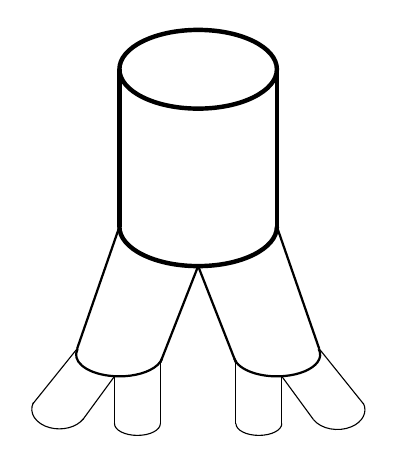
\begin{tikzpicture}[scale=0.5]
			\draw[ultra thick] (0,0) ellipse (2 and 1);
			\draw[ultra thick] (-2,0)--(-2,-4);
			\draw[ultra thick] (2,0)--(2,-4);
			\draw[ultra thick] ($(0, -4) + (180:2cm and 1cm)$(P) arc  (180:360:2cm and 1cm);
			\draw[thick] (-2,-4)--(-3.075,-7.1);
			\draw[thick] (0,-5)--(-0.96,-7.45);
			\draw[thick] ($(-2, -7.25) + (165:1.1cm and 0.55cm)$(P) arc  (165:350:1.1cm and 0.55cm);
			\draw[thick] (2,-4)--(3.075,-7.1);
			\draw[thick] (0,-5)--(0.96,-7.45);
			\draw[thick] ($(2, -7.25) + (190:1.1cm and 0.55cm)$(P) arc  (190:375:1.1cm and 0.55cm);
			\draw (-3.075,-7.1)--(-4.2,-8.5);
			\draw (-2.125,-7.8)--(-2.93,-8.9);
			\draw ($(-3.62, -8.6) + (160:0.6cm and 0.4cm)$(P) arc  (160:330:0.7cm and 0.5cm);
			\draw (-2.125,-7.8)--(-2.125,-9);
			\draw (-0.96,-7.45)--(-0.96,-9);
			\draw ($(-1.5425, -9) + (180:0.5825cm and 0.3cm)$(P) arc  (180:360:0.5825cm and 0.3cm);
			
			\draw (3.075,-7.1)--(4.2,-8.5);
			\draw (2.125,-7.8)--(2.93,-8.9);
			\draw ($(3.45, -8.7) + (210:0.6cm and 0.4cm)$(P) arc  (210:380:0.7cm and 0.5cm);
			\draw (2.125,-7.8)--(2.125,-9);
			\draw (0.96,-7.45)--(0.96,-9);
			\draw ($(1.5425, -9) + (180:0.5825cm and 0.3cm)$(P) arc  (180:360:0.5825cm and 0.3cm);
		\end{tikzpicture}
	\end{center}
		The first segment is very large, then it bifurcates into smaller segments in a geometrical pattern.
		
		Here is some data about human lungs:
		\begin{itemize}
			\item radius of first segment: $r_0 = 0.5$cm
			\item length of first segment: $\ell_0 = 5.6$cm
			\item ratio of daughter to parent length: $\alpha = 0.9$
			\item ratio of daughter to parent radius: $\beta = 0.86$
			\item number of branch generations: $M=30$
			\item average number of daughters per parent: $b = 1.7$
		\end{itemize}
		
		In the figure, there are 2 daughters per parent, in 	real lungs, it isn't perfectly regular, so we have an average that is not a whole number.
		
		
		
	\item Calculate the volume inside the segments. What is the limit as the number of segments gets larger and larger?
	\item Calculate the surface area inside the segments. What is the limit as the number of segments gets larger and larger?

	\item If we had $b=2$ instead and the same number of generations, would that be possible? If not, how many generations would be possible?
\end{enumerate}


%\vfill
\newpage
\emph{Task 2. } Let us model the gas exchange that happens inside the lungs.
\begin{enumerate}[label=\emph{(\alph*)}]
\item Suppose that a lung has a volume of 3L when full. With each breath, 0.6L of the air is exhaled and replaced by 0.6L of outside air.

	After exhaling the volume is 2.4L and it returns to 3L after inhaling.
	
	Suppose further that the lung contains a chemical with a concentration of 2 milimoles per litre before exhaling (a mole is a chemical unit for $6.02 \times 10^{23}$ molecules). The ambient air has a concentration of 5mmol/L of the same chemical.

	What is the concentration after one breath? What is the concentration after $n$ breaths?

\item Update your model to match the oxygen exchange inside a real human lung.
	
\item The model above ignored the fact that the body absorbs some of the oxygen. Assume now that the lungs absorb 30\% of the oxygen with each breath. Update your model.

\item What is the equilibrium concentration of oxygen in the lungs? Find the graph of the equilibrium concentration as a function of the fraction of oxygen absorbed with each breath.

\end{enumerate}

\begin{graybox}
You may choose to model the gas exchange in the lungs using either a discrete time \emph{difference equation} or a continuous time \emph{differential equation}.
	\begin{enumerate}[label=\emph{(\alph*)}]
	\item If you choose a difference equation, you might assume that every breath the concentration of the chemical changes. If $c(n)$ or $c_n$ represented the concentration of chemical after $n$ breaths, your difference equation might look like
	\begin{itemize}
		\item $\Delta c(n) = c(n) - c(n-1) =$ some function at time $n$, where $n$ is only allowed to take whole numbers.
	\end{itemize}

	\item If you choose to use differential equations, the analogous equation would look like
	\begin{itemize}
		\item $c'(t)=$ some function at $t$, where $t$ can take any positive real value.  
	\end{itemize}
\end{enumerate}
\end{graybox}

\vfill

\emph{Task 3. } Assume that the lungs only absorb a fraction of the air in contact with its surface. Combine the two previous tasks.

\vfill

\emph{Further Investigation:}
\begin{enumerate}[label=\emph{\arabic*.}]
%	\item Assume that the lungs only absorb a fraction of the air in contact with its surface. Combine the two tasks.
	\item Investigate how the what is known about human lungs. Compare how the branching of real human lungs differs from this model. Refine the estimate.
	\item Investigate how the what is known about human lungs. Compare how the gas exchange of real human lungs differs from this model. Refine the model.
\end{enumerate}

\vspace{1cm}


\begin{graybox}
\hfill ``\lungstitle'' is a collaboration with Kseniya Garaschuk and Miroslav Lovric.
\end{graybox}
\begin{noexercises}
\end{noexercises}

\end{project}








%%%%%%%%%%%%%%%%%%%%%%%%%%%%%%
%
%  Project - Zombies
%
%%%%%%%%%%%%%%%%%%%%%%%%%%%%%%



\begin{project}{Dark day}
	\label{proj:zombies}

	\begin{emphbox}[]
	At one in the morning, your phone goes off.  After three attempts to 
	turn off your alarm clock, you finally realize that it is a call -- -a call from a 
	number you had promised to always answer.  By 1:15, you're dressed and out the door where 
	a black SUV is idling, waiting for you.  After a transfer to a government plane, you 
	touch down in Washington, D.C., and as the sun finally begins to rise, you traverse 
	down the Secret Service tunnels to a large conference room lined with leather chairs.

	``I'm not going to mince words,'' a voice says, from the other side of the room.  The 
	chair at the end of the table swivels round and you see the President emerge 
	from the shadows.  ``It's bad.  It's worse than bad.  It's, uh\ldots it's zombies.''

	A revelation like that would have thrown a lesser scientist, but you're a professional.  
	You've been preparing for this for years, urging your colleagues to take the threat seriously.  

	``Where is the origin?  Have we identified a patient zero in the US or are there multiple sources?  
	What are the parameters of the disease\mbox{?}'' you ask.

	``Straight to work, okay,'' the President says, looking pleased. ``Chicago police began reporting violent attacks a few days ago.  It started with a single report in the navy shipyard.  The shipyard has been quarantined, but we're now getting reports from all over the city. These attacks are carried out by humans who always attempt to bite their victims.  Those bitten begin to show symptoms within a matter of hours, but those who are attacked but escape without being bitten appear normal. I've sent in the Marines, and they estimate that an infected person dies after eight days. They also predict about 3,000 individuals have been exposed, five days 	after the initial report.''

	``Has any quarantine been successful\mbox{?}'' you ask.

	``No.''  The President pauses and the gravity of what he has just said starts to sink in.  
	``There are approximately 9.7 million people living in the Chicago metro area.  Obviously 
	time is of the essence.  Now, I've been told that you're the best epidemiologist we have.  
	I need to know if the region has a chance of survival, and if it does, what the impact will be.
	Is there any hope for Chicago?''
\end{emphbox}


%\vfill

\begin{graybox}
You may choose to model the zombie outbreak using either a discrete time \emph{difference equation} or a continuous time \emph{differential equation}.
	\begin{enumerate}[label=\emph{(\alph*)}]
		\item If you choose a difference equation, you might assume that every day or every hour, the number of zombies, humans, and dead increment.  If $Z(n)$ represented the number of zombies at time $n$, one of your difference equations might look like
%	\[
%		\Delta Z(n) = Z(n) - Z(n-1) = \text{some function of zombies, humans, and dead at time $n$},
%	\]
\begin{itemize}
	\item $\Delta Z(n) = Z(n) - Z(n-1) =$ some function of zombies, humans, and dead at time $n$,
	where $n$ is only allowed to take whole numbers.
\end{itemize}

	\item If you choose to use differential equations, the analogous equation would look like
%	\[
%		Z'(t) = \text{some function of zombies, humans, and dead at time $t$},
%	\]
\begin{itemize}
	\item $	Z'(t) = $ some function of zombies, humans, and dead at time $t$,
	where $t$ can take any positive real value.  
\end{itemize}

	\item Modelling with a difference equation or a differential equation should give you similar results (why?).
	\end{enumerate}
	
\end{graybox}

%\newpage
\emph{Task.} Model the zombie infection. Make sure to address the following in your report:
	\begin{enumerate}[label=\emph{(\alph*)}]
		\item What situation are you trying to model?
		\item What equations are you using, and what does each variable in each equation represent
			(for example, ``In this model, $Z(t)$ is the number of zombies at $t$ hours from initial outbreak).
		\item Justification for any constants that you use and how you estimated them.
		\item Is there any hope for Chicago?
	\end{enumerate}

Do not attempt to find an equation that solves your differential equations---this is really hard.
Instead, rely on estimates and simulations.  You can use any computer program you like to assist you in estimating how the zombie outbreak spreads and whether your constants match with the known information.  Including plots and figures in your report will make explaining things easier.



\vfill

\begin{graybox}
\hfill ``\zombiestitle'' is a collaboration with Max Brugger.
\end{graybox}

\begin{noexercises}
\end{noexercises}
\end{project}






\end{bookonly}







%%%%%%%%%%%%%%%%%%%%%%%%%%%%%%%%%%%%%%%%%%%%%%%%%%%%%%%%%%%%%%%%%%%%%%%%
%
%		Appendices
%
%%%%%%%%%%%%%%%%%%%%%%%%%%%%%%%%%%%%%%%%%%%%%%%%%%%%%%%%%%%%%%%%%%%%%%%%



\begin{bookonly}
%\appendix


\begin{topic}[Appendix]

\vfil
\begin{center}
\begin{minipage}{175pt}
	\includegraphics*[width=175pt]{images/appendix-xkcd.png}

	\hfill {\footnotesize (image from \href{https://www.xkcd.com/1050/}{xkcd - comic \#1050})}
\end{minipage}
\end{center}


\end{topic}




\subsection{Linear Algebra Review}
\label{LinAlg}

\begin{center}\textbf{\color{cyan}Algebra of Solving Systems of 2 Linear Equations} 	
\end{center}

We can write a linear system of equations 
\begin{align*}
a_{11} x_1 + a_{12} x_2 &= b_1 \\
a_{21} x_1 + a_{22} x_2 &= b_2
\end{align*}
into matrix form
$$
{\bf A} \vec{x} = \vec{b},
$$
where
$$
{\bf A} 
	= \begin{pmatrix} 
		a_{11} & a_{12} \\
		a_{21} & a_{22}
	\end{pmatrix}
	\quad \text{,} \quad 
\vec{x}  
	= \begin{pmatrix} 
		x_{1} \\
		x_{2} 
	\end{pmatrix}
	\quad \text{ and } \quad 
\vec{b}  
	= \begin{pmatrix} 
		b_{1} \\
		b_{2} 
	\end{pmatrix} .
$$

We can solve a system like this one in several different ways.

\begin{example}
Solve the system
\begin{align*}
3x_1+2x_2 &= 7 \\
2x_1+3x_2 & = 8.
\end{align*}
\end{example}

\begin{definition}[Solution by substitution.] 
We can write
$$
x_2 = \frac{7-3x_1}{2},
$$
and use this on the second equation
$$
2x_1 + 3\frac{7-3x_1}{2} = 8
	\quad \Leftrightarrow \quad 4x_1 + 21-9x_1=16
	\quad \Leftrightarrow \quad -5x_1 =-5
	\quad \Leftrightarrow \quad x_1 =1
$$
Then re-use the first equation we obtained to get $x_2 = 2$.
	
\end{definition}

\begin{definition}[Solution by Cramer's rule]
	
Using the same method of substitution on the general system, we obtain
$$
a_{12} x_2 = b_1 - a_{11} x_1,
$$
and we use this into the second equation (after multiplying by $a_{12}$)
$$
a_{12} a_{21} x_1 = a_{22} b_1 - a_{11}a_{22} x_1 = a_{12} b_2
$$
This implies 
$$
x_1 
	= \frac{b_1 a_{22} - a_{12} b_2}{a_{11}a_{22} - a_{12}a_{21}}
	= \frac{
		\begin{vmatrix} 
			b_1 & a_{12} \\
			b_2 & a_{22}
		\end{vmatrix}
		}{
		\begin{vmatrix} 
			a_{11} & a_{12} \\
			a_{21} & a_{22}
		\end{vmatrix}
		}
$$
Then we use this to obtain
$$
x_2
	= \frac{a_{11} b_2  - b_1 a_{21} }{a_{11}a_{22} - a_{12}a_{21}}
	= \frac{
		\begin{vmatrix} 
			a_{11} & b_1 \\
			a_{21} & b_2
		\end{vmatrix}
		}{
		\begin{vmatrix} 
			a_{11} & a_{12} \\
			a_{21} & a_{22}
		\end{vmatrix}
		}
$$

\end{definition}

\begin{important}
This implies that there is a unique solution of the system if and only if
$$
\det ({\bf A}) = a_{11}a_{22} - a_{12}a_{21} \neq 0.
$$
\end{important}



\begin{definition}[Solution by inverse matrix]
 A matrix is {\bf invertible} or {\bf nonsingular} \quad iff \quad ${\bf A}^{-1}$ exists \quad iff \quad $\det({\bf A}) \neq 0$.

If the matrix {\bf A} is invertible, then we can write
$$
{\bf A}^{-1} 
	= \frac{1}{\det({\bf A})} \begin{pmatrix}
						a_{22} & -a_{12} \\
						-a_{21} & a_{11}
						\end{pmatrix}
$$

We can now use this to solve the system of equations:
\begin{align*}
{\bf A} \vec{x}	& = \vec{b}  \\
{\bf A}^{-1} {\bf A} \vec{x}	& = {\bf A}^{-1} \vec{b}  \\
{\bf I} \vec{x}	& = {\bf A}^{-1} \vec{b}  \\
\vec{x}	& = {\bf A}^{-1} \vec{b}
\end{align*}

\end{definition}





\begin{definition}[Homogeneous Systems]
	
A system of equations is called \emph{homogeneous} if $\vec{x}=\vec{0}$ is a solution, which means that $\vec{b} = 0$:
$$
{\bf A} \vec{x} = \vec{0}.
$$

Otherwise, it is called \emph{nonhomogeneous}.
\end{definition}



\hfil







\begin{center}\textbf{\color{cyan}Eigenvalues and Eigenvectors} 	
\end{center}


We can think of the matrix multiplication $\vec{y}={\bf A}\vec{x}$ as a mapping or transformation: given a vector $\vec{x}$ it transforms it into a different vector $\vec{y}$.

In many applications, it is important to know which vectors $\vec{x}$ are transformed into multiples of themselves.

These vectors satisfy the property
$$
{\bf A}\vec{x} = \lambda \vec{x} \qquad \Leftrightarrow \qquad ({\bf A} - \lambda {\bf I} ) \vec{x} = \vec{0}.
$$

One such vector is $\vec{x}=\vec{0}$. But that's not very interesting. We want to look for nonzero vectors that satisfy this property.

These vectors are called {\bf eigenvectors} and the corresponding $\lambda$ is called an {\bf eigenvalue}.

\begin{important}
The second formulation above implies that the matrix $({\bf A} - \lambda {\bf I})$ is singular, otherwise the unique solution would be $\vec{x}=\vec{0}$. 
So that implies that 
\begin{equation}\tag{\bf characteristic equation}
\det({\bf A} - \lambda {\bf I}) = 0
\end{equation}
\end{important}



\begin{example}
Let us find the eigenvalues and eigenvectors for
$$
{\bf A} = \begin{pmatrix} 1 & 8 \\ 4 & 5 \end{pmatrix}.
$$

First we solve the characteristic equation:
$$
\det({\bf A} - \lambda {\bf I}) 
	= \begin{vmatrix}
		1 - \lambda & 8 \\	
		4 & 5 - \lambda
	\end{vmatrix}
	= (1-\lambda)(5-\lambda) - 32 = 0
\qquad \Leftrightarrow \qquad
	\lambda^2 - 6 \lambda -27=0
$$
which implies that
$$
\lambda = 3 \pm \sqrt{9 + 27} = 3 \pm 6
$$


\subparagraph{Eigenvalue $\lambda_1 = -3$. } To find the eigenvector, we write its equation
$$
({\bf A} - \lambda_1 {\bf I} ) \vec{x} = \vec{0}
\qquad \Leftrightarrow \qquad
\begin{pmatrix}
	4 & 8 \\
	4 & 8
\end{pmatrix}
\begin{pmatrix}
x_1 \\ x_2 
\end{pmatrix}
	= \begin{pmatrix}
	0 \\ 0
	\end{pmatrix}
$$
which implies that
$$
4x_1 +8x_2 = 0
\qquad \Leftrightarrow \qquad
x_1 = -2 x_2.
$$
So one eigenvector for this eigenvalue is
$$
\vec{x}_1 = \begin{pmatrix}
	-2 \\ 1
	\end{pmatrix}
$$


\subparagraph{Eigenvalue $\lambda_2 = 9$. } To find the eigenvector, we write its equation
$$
\begin{pmatrix}
	-8  & 8 \\
	4 & -4
\end{pmatrix}
\begin{pmatrix}
x_1 \\ x_2 
\end{pmatrix}
	= \begin{pmatrix}
	0 \\ 0
	\end{pmatrix}
$$
which implies that
$$
-8x_1 +8x_2 = 0
\qquad \Leftrightarrow \qquad
x_1 = x_2.
$$
So one eigenvector for this eigenvalue is
$$
\vec{x}_2 = \begin{pmatrix}
	1 \\ 1
	\end{pmatrix}
$$
\end{example}





\begin{theorem}
Let {\bf A} have real or complex eigenvalues $\lambda_1$ and $\lambda_2$ such that $\lambda_1 \neq \lambda_2$ and let the corresponding eigenvectors be
$$
\vec{x}_1 = \begin{pmatrix} x_{11}  \\ x_{21} \end{pmatrix}
\qquad \text{ and } \qquad
\vec{x}_2 = \begin{pmatrix} x_{12}  \\ x_{22} \end{pmatrix}.
$$
If {\bf X} is the matrix with columns taken from the eigenvectors:
$$
{\bf X} = \begin{pmatrix}
x_{11} & x_{12} \\
x_{21} & x_{22}
\end{pmatrix},
$$
then 
$$\det({\bf X}) \neq 0.$$
\end{theorem}









\subsection{Mathematical Induction Review}
\label{app:induction}






Mathematical induction is a very powerful tool for proving results. It allows us to prove generalized results. 
Its shortcoming is that you already have to suspect what the solution is. It then allows you to prove it.


\begin{definition}[The Principle of Mathematical Induction]
	
Assume that ${\bf P}(1)$, ${\bf P}(2)$, ${\bf P}(3), \ldots$ is an infinite sequence of mathematical statements. \\

\begin{tabular}{ll|ll}
{\bf If}  & & {\bf If} \\
	& (a) \quad ${\bf P}(1)$ is true, 		& & first domino falls \\
	& 	{\bf and} & & {\bf and} \\
	& (b) \quad  for any $k$, ${\bf P}(k)$ implies ${\bf P}(k+1)$ 	
		& & if a domino falls, then the next one falls \\
{\bf then} & & & {\bf then} \\
	& all the statements in the sequence are true	& & all dominoes fall!
\end{tabular}

\end{definition}


\begin{example}
For any $n\in \N$, $1+3+5+\cdots+(2n-1) = n^2$. \\

Let us prove this formula using Mathematical Induction.

\paragraph{Proof.}
If $n=1$, we get $1=1^2$, which is true -- ${\bf P}(1)$ holds.

Assume that $1+3+5+\cdots+(2k-1) = k^2$ for some $k$.
Then
\begin{align*}
1+3+5+\cdots+\big(2(k+1)-1\big) 
	& = \underbrace{1+3+5+\cdots+(2k-1)}_{= k^2 \text{ by induction hypothesis}} + (2k+1) \\
	& = k^2+(2k+1)\\
	& = k^2 + 2k + 1\\
	& = (k+1)^2.
\end{align*}
By induction, the equality holds for all $n\in \N$.

\end{example}


\begin{example}
	
For any $x\in \R$ with $x\geq -1$ and $n \in \N$, then $(1+x)^n \geq 1+nx$. \hfill (Bernoulli's Inequality)

\paragraph{Proof.}
For $n=1$, $1+x\geq 1+x$, which is true!

Assume that $(1+x)^k \geq 1+kx$. Then
\begin{align*}
(1+x)^{k+1} 
	& = (1+x)^k (1+x) 
		\geq (1+kx)(1+x) \\
	& = 1 + x + kx^2 + kx 
		= 1+(k+1)x+kx^2 \\
	& \geq 1+(k+1)x.
\end{align*}
By induction, the claim holds for all $n \in \N$.

\begin{graybox}
	
In the proof, we didn't use the fact that $x\geq -1$, but 
for $n=3$ and $x=-4$, $(1+x)^n = -27 \not\geq -11 = 1+nx$.  \\

Where did we use the hypothesis $x\geq -1$?
\end{graybox}

\end{example}






%%%%%%%%%%

\newpage

\begin{definition}[Principle of Strong Mathematical Induction]

Assume that ${\bf P}(1)$, ${\bf P}(2)$, ${\bf P}(3), \ldots$ is an infinite sequence of mathematical statements. \\

\begin{tabular}{lll|ll}
{\bf If} & & & {\bf If} \\
	& (a) & ${\bf P}(1)$ is true, 		 & & first domino falls \\
	&  {\bf and} & & & {\bf and} \\
	& (b) &  For any $k$, ${\bf P}(1), \ldots, {\bf P}(k)$ implies ${\bf P}(k+1)$ 	& & if all previous dominos fell, \\
	& & & & then the next one falls \\
{\bf then} & & & {\bf then} \\
	& \multicolumn{2}{l|}{all the statements in the sequence are true} & & all dominoes fall!
\end{tabular}

\end{definition}


\begin{example}
\begin{theorem}
Every number $n\in\N, n\geq 2$ can be written as a product of primes (or is a prime).
\end{theorem}

\paragraph{Proof.}
Base case: $n=2$ is a prime.

Assume that the Theorem holds for $n=2,3,4,\ldots, k$ and consider $n=k+1$.

If $k+1$ is prime, the claim holds.

If $k+1$ is not a prime, then it is divisible by some $2 \leq m \leq k$: $k+1=m\cdot \ell$ for some $2 \leq m,\ell\leq k$.
By hypothesis, both $m$ and $\ell$ are products of primes, hence so is $k+1$.
The Theorem follows by strong induction.
\end{example}




%\begin{ex} How many cuts are needed to cut a chocolate bar with $n$ squares into $1\times 1$ pieces?
%\end{ex}
%
%\paragraph{Claim: } $n-1$ cuts are needed to separate $n$ squares. \\
%
%\begin{minipage}{12cm}
%\begin{proof}
%For $n=1$, no cuts are needed, so the claim holds.
%
%Assume that the claim holds for $n=1,2,3,\ldots,k$ and consider a bar with $k+1$ squares.
%Perform one cut to obtain smaller bars with $m$ and $\ell$ squares (so $k+1=m+\ell$).
%By assumption, $m-1$ and $\ell-1$ are needed to cut the smaller bars, so to cut the original bar, we need
%$$
%1 + m-2+\ell-1 = m + \ell -1 = k
%$$
%The claim holds for $n=k+1$, so by strong induction it holds for all $n\in\N$.
%\end{proof}
%\end{minipage}
%\qquad
%\begin{minipage}{125pt}
%\includegraphics*[width=100pt]{figures/chocobar.pdf}
%\end{minipage}
%
%
%
%\begin{thm}
%Every $n\in \N$ can be written as a sum of distinct nonnegative integer powers of $2$.
%\end{thm}
%
%\begin{ex}
%\begin{align*}
%17 & = 2^0 + 2^4 \\
%42 & = 2^1 + 2^3+ 2^5 \\
%65 & = 2^0 + 2^6
%\end{align*}
%\end{ex}
%
%\begin{proof}
%The Theorem holds for $n=1$, since $1 = 2^0$.
%
%Assume that it works for $n=1,2,\ldots, k$ and consider $n=k+1$.
%
%If $k$ is even then by assumption $k=2^{a_1} + 2^{a_2} + \cdots + 2^{a_\ell}$ for $0<a_1<a_2<\cdots<a_\ell$ and 
%$$
%k+1 = 2^0 + 2^{a_1} + 2^{a_2} + \cdots + 2^{a_\ell}
%$$
%is the required representation.
%
%If $k$ is odd, then $k+1$ is even, hence $k+1=2 m$ for some $m\in \N$. By assumption, $m=2^{a_1} + 2^{a_2} + \cdots + 2^{a_\ell}$ for some $0\leq a_1<a_2<\cdots<a_\ell$ and hence
%$$
%k+1 = 2^{a_1+1} + 2^{a_2+1} + \cdots + 2^{a_\ell+1}.
%$$
%By strong induction, the Theorem follows.
%\end{proof}
%
%




%%%%%%%%%%%%%%%%%%%%%%%%%%%%%%%%%%%%%%%%%%%%%%%%%%%%%%%%%%%%%
%
%	practice problems
%
%%%%%%%%%%%%%%%%%%%%%%%%%%%%%%%%%%%%%%%%%%%%%%%%%%%%%%%%%%%%%

\begin{exercises}
		% Topics:
		% 
	\begin{problist}
		% 
		\prob Is the triangle inequality true for more than two numbers?
			$$
			|x_1 + x_2 + \cdots + x_n| \stackrel{?}{\leq} |x_1| + |x_2| + \cdots + |x_n| 
			$$
			If it is, prove it.
			
		\prob Is the AGM inequality true for any $x_1, x_2, \ldots, x_n \geq 0$?
			$$
			\sqrt{x_1 x_2 \cdots x_n} \stackrel{?}{\leq}\frac{x_1 + x_2 + \cdots + x_n}{n}
			$$
			If it is, prove it.
			
		\prob Prove that for any $n \in \N$, $2^{6n}+3^{2n-2}$ is divisible by $5$.


		\prob How many subsets does a set $S$ with $n$ elements have (including $S$ and $\emptyset$)?
		
		\prob Show that If $x_1, \ldots, x_n \in [0,1]$ then $\displaystyle \prod_{i=1}^n (1-x_i) \geq 1 - \sum_{i=1}^n x_i$

		\prob Can you use Mathematical induction to prove that $P(m), P(m+1), P(m+2),\ldots$ are true? If so, how?

		\prob Can you use Mathematical induction to prove that $P(2), P(4), P(6), P(8), \ldots$ are true? If so, how?

		\prob Can you use Mathematical induction to prove that $P(1), P(3), P(5), P(7), \ldots$ are true? If so, how?

		\prob For which $n \in \N$, $2^n \geq (n+1)^2$? Prove your answer.

		\prob Show that for even $n$'s, $n(n^2+3n+2)$ is divisible by $24$.

		\begin{center}
			\includegraphics*[width=15pt]{images/app-ind-L-shape.pdf}
		\end{center}
		\prob Prove that for any $n \in \N$, a $2^n \times 2^n$ checkerboard with one single square removed has an L--tiling (i.e., can be covered with L--shapes).
%
%{\it Proof. } 
%For $k=1$, a $2\times 2$ board with one square removed has an L--shape, so it can be covered with a single L.
%
%Assume for $k$ and prove for $k+1$:
%
%\begin{minipage}{10cm}
%Divide the board in 4 $2^k \times 2^k$ boards. One of the smaller boards will have a square missing.
%
%Remove three squares from the centre from each of the other 3 boards - forming an L--shape as in the figure.
%We then have 4 boards with dimensions $2^k \times 2^k$ with one square removed.
%
%By induction hypothesis, we can cover each of these boards with L--shapes and we can cover the middle gap with one L--shape.
%Therefore the $2^{k+1} \times 2^{k+1}$ board has an L--tiling, and the claim follows by induction. \qed
%\end{minipage}
%\quad
%\begin{minipage}{150pt}
%\includegraphics*[width=150pt]{images/app-ind-2k1_board.pdf}
%\end{minipage}

		\prob Read the following proof:
		
		\begin{theorem} All horses have the same colour.
		\end{theorem}
		
		\begin{graybox}
			
		\paragraph{Proof.}
		Assume that the claim holds for groups of $k$ horses, and consider a group with $k+1$ horses $S = \{h_1, \ldots, h_{k+1}\}$.\\
		
		By hypothesis, the horses in $A = \{h_1,\ldots, h_k\}$ and $B = \{h_2, \ldots, h_{k+1}\}$ have the same colour. Since the horse $h_2$ is in both groups, we deduce that the colour of the horses in $A$ must be the same as of these in $B$.  \\
		
		In conclusion, the horses in $S = A \cup B$ must have the same colour, and the claim holds by induction.	
		\end{graybox}
		
		This proof is flawed. Explain how.
		


%
%\paragraph{The proof above is FALSE: } 
%For $k=1$, $k+1=2$ and $A = \{h_1\}$ and $B = \{h_2\}$, so there are no common horses to $A$ and $B$ an the argument that the colour in $A$ is the same as in $B$ fails!
%
%(it's like we proved that the first domino falls and if a domino falls the next one also falls, except the second one never falls!)

		
	\end{problist}
\end{exercises}




%\subsection{2019 $M_3C$ competition report from the winning team}
\label{2019M3C}

%\hspace{-0.5cm}\includegraphics*[page=1,scale=0.9]{example/Vaping-abridged.pdf}
%
%\newpage

\begin{minipage}{.7\textwidth}
In the following pages you can find an abridged version of the full report. The full report can be found at \url{https://uoft.me/modelling-app-report}.	
\end{minipage}
\hfill
\begin{minipage}{.25\textwidth}
	\qrcode{https://uoft.me/modelling-app-report}
\end{minipage}


	\vfil

	\hfil \framebox{\includegraphics*[scale=0.67]{example/Vaping-cover.pdf}}

\newpage

\forLoop[1]{1}{12} % variable is \i
{
	\hfil\\
	\vfil
	\hfil \framebox{\includegraphics*[page=\i,scale=0.85]{example/Vaping-abridged.pdf}}
	\newpage
}




\end{bookonly}

\end{document}
